% !TeX document-id = {e3a7ff19-e925-4f85-9d15-87fd720805e2}
% ******************************* PhD Thesis Template **************************
% Please have a look at the README.md file for info on how to use the template

\documentclass[a4paper,12pt,times,numbered,print,index,square, sort, numbers, authoryear]{Classes/PhDThesisPSnPDF}

% ******************************************************************************
% ******************************* Class Options ********************************
% *********************** See README for more details **************************
% ******************************************************************************

% `a4paper'(The University of Cambridge PhD thesis guidelines recommends a page
% size a4 - default option) or `a5paper': A5 Paper size is also allowed as per
% the Cambridge University Engineering Deparment guidelines for PhD thesis
%
% `11pt' or `12pt'(default): Font Size 10pt is NOT recommended by the University
% guidelines
%
% `oneside' or `twoside'(default): Printing double side (twoside) or single
% side.
%
% `print': Use `print' for print version with appropriate margins and page
% layout. Leaving the options field blank will activate Online version.
%
% `index': For index at the end of the thesis
%
% `draft': For draft mode without loading any images (same as draft in book)
%
% `abstract': To generate only the title page and abstract page with
% dissertation title and name, to submit to the Student Registry
%
% ************************* Custom Page Margins ********************************
%
% `custommargin`: Use `custommargin' in options to activate custom page margins,
% which can be defined in the preamble.tex. Custom margin will override
% print/online margin setup.
%
% *********************** Choosing the Fonts in Class Options ******************
%
% `times' : Times font with math support. ( The Cambridge University guidelines
% recommend using times)
%
% `fourier': Utopia Font with Fourier Math font
%
% `customfont': Use `customfont' option in the document class and load the
% package in the preamble.tex
%
% default or leave empty: `Latin Modern' font will be loaded.
%
% ********************** Choosing the Bibliography style ***********************
%
% `authoryear': For author-year citation eg., Krishna (2013)
%
% `numbered': (Default Option) For numbered and sorted citation e.g., [1,5,2]
%
% `custombib': Define your own bibliography style in the `preamble.tex' file.
% `\RequirePackage[square, sort, numbers, authoryear]{natbib}'
%
% **************************** Choosing the Page Style *************************
%
% `default (leave empty)': For Page Numbers in Header (Left Even, Right Odd) and
% Chapter Name in Header (Right Even) and Section Name (Left Odd). Blank Footer.
%
% `PageStyleI': Chapter Name next & Page Number on Even Side (Left Even).
% Section Name & Page Number in Header on Odd Side (Right Odd). Footer is empty.
%
% `PageStyleII': Chapter Name on Even Side (Left Even) in Header. Section Number
% and Section Name in Header on Odd Side (Right Odd). Page numbering in footer


% ********************************** Preamble **********************************
% Preamble: Contains packages and user-defined commands and settings

\usepackage{etoolbox}
\usepackage{rotating}


\usepackage{/usr/local/texlive/texmf-local/picins/picins}

\usepackage{graphicx}
\usepackage{algorithm}
\usepackage{algpseudocode}
\usepackage{needspace}
\usepackage{multirow}
\usepackage{afterpage}
\usepackage{wrapfig}


% ******************************************************************************
% ****************************** Custom Margin *********************************
% Add `custommargin' in the document class options to use this section
% Set {innerside margin / outerside margin / topmargin / bottom margin}  and
% other page dimensions
\ifsetMargin
\else
    \RequirePackage[left=37mm,right=30mm,top=35mm,bottom=30mm]{geometry}
    \setFancyHdr % To apply fancy header after geometry package is loaded
\fi

% *****************************************************************************
% ******************* Fonts (like different typewriter fonts etc.)*************

% Add `customfont' in the document class option to use this section
\ifsetFont
\else
    % Set your custom font here and use `customfont' in options. Leave empty to
    % load computer modern font (default LaTeX font).  
    \RequirePackage{libertine} 
\fi

% *****************************************************************************
% *************************** Bibliography  and References ********************

%\usepackage{cleveref} %Referencing without need to explicitly state fig /table

% Add `custombib' in the document class option to use this section
\ifsetBib % True, Bibliography option is chosen in class options
\else % If custom bibliography style chosen then load bibstyle here
    \RequirePackage[square, sort, numbers, authoryear]{natbib} % CustomBib
\fi

% changes the default name `Bibliography` -> `References'
\renewcommand{\bibname}{References}

% *****************************************************************************
% *************** Changing the Visual Style of Chapter Headings ***************
% Uncomment the section below. Requires titlesec package.

%\RequirePackage{titlesec}
%\newcommand{\PreContentTitleFormat}{\titleformat{\chapter}[display]{\scshape\Large}
%{\Large\filleft{\chaptertitlename} \Huge\thechapter}
%{1ex}{}
%[\vspace{1ex}\titlerule]}
%\newcommand{\ContentTitleFormat}{\titleformat{\chapter}[display]{\scshape\huge}
%{\Large\filleft{\chaptertitlename} \Huge\thechapter}{1ex}
%{\titlerule\vspace{1ex}\filright}
%[\vspace{1ex}\titlerule]}
%\newcommand{\PostContentTitleFormat}{\PreContentTitleFormat}
%\PreContentTitleFormat


% *****************************************************************************
% **************************** Custom Packages ********************************
% *****************************************************************************


% ************************* Algorithms and Pseudocode **************************

%\usepackage{algpseudocode} 


% ********************Captions and Hyperreferencing / URL **********************

% Captions: This makes captions of figures use a boldfaced small font. 
%\RequirePackage[small,bf]{caption}

\RequirePackage[labelsep=space,tableposition=top]{caption} 
\renewcommand{\figurename}{Fig.} %to support older versions of captions.sty


% ************************ Formatting / Footnote *******************************

%\usepackage[perpage]{footmisc} %Range of footnote options 


% ****************************** Line Numbers **********************************

%\RequirePackage{lineno}
%\linenumbers

% ************************** Graphics and figures *****************************
\usepackage[help]{epspdfconversion}
\usepackage{epstopdf}
%\usepackage{rotating}
%\usepackage{wrapfig}
%\usepackage{float}
\usepackage{subfig} %note: subfig must be included after the `caption` package. 

% ********************************* Table **************************************

%\usepackage{longtable}
%\usepackage{multicol}
%\usepackage{multirow}
%\usepackage{tabularx}


% ***************************** Math and SI Units ******************************

\usepackage{amsfonts}
\usepackage{amsmath}
\usepackage{amssymb}
%\usepackage{siunitx} % use this package module for SI units


% ******************************************************************************
% ************************* User Defined Commands ******************************
% ******************************************************************************


% ********************** TOC depth and numbering depth *************************
% ******** We need subsubsubsections *********
\setcounter{secnumdepth}{4}
\setcounter{tocdepth}{3}

% ******************************* Nomenclature *********************************

% To change the name of the Nomenclature section, uncomment the following line

%\renewcommand\nomname{Symbols}


% ********************************* Appendix ***********************************

% The default value of both \appendixtocname and \appendixpagename is `Appendices'. These names can all be changed via: 

%\renewcommand{\appendixtocname}{List of appendices}

%\renewcommand{\appendixname}{Appndx}

\usepackage{notation-private}
\usepackage{animate}
\usepackage{media9}
\usepackage{subfig}

\epstopdfsetup{outdir=Figs/PDF/}
\ifpdf
    \graphicspath{{Figs/Raster/}{Figs/PDF/}{Figs/}}
\else
    \graphicspath{{Figs/Vector/}{Figs/}}
\fi

% ************************ Thesis Information & Meta-data **********************
%% The title of the thesis
\title{A Fingertip Mechanical-Stress Detector using Chromatic Skin Information}
%\texorpdfstring is used for PDF metadata. Usage:
%\texorpdfstring{LaTeX_Version}{PDF Version (non-latex)} eg.,
%\texorpdfstring{$sigma$}{sigma}

%% The full name of the author
\author{Nayef Al-Saud}

%% Department (eg. Department of Engineering, Maths, Physics)
\dept{Department of Engineering}

%% University and Crest
\university{University of Cambridge}
\crest{
\includegraphics[width=0.25\textwidth]{Figs/University_Crest.pdf}}

%% You can redefine the submission text:
% Default as per the University guidelines: This dissertation is submitted for
% the degree of Doctor of Philosophy
%\renewcommand{\submissiontext}{change the default text here if needed}

%% Full title of the Degree
\degree{Master of Philosophy in Engineering}

%% College affiliation (optional)
\college{Hughes Hall}

%% Submission date
\degreedate{17 February 2014}

%% Meta information
\subject{LaTeX} \keywords{{LaTeX} {MPhil Thesis} {Engineering} {University of
Cambridge}}



% ***************************** Abstract Separate ******************************
% To printout only the titlepage and the abstract with the PhD title and the
% author name for submission to the Student Registry, use the abstract option in
% the document class.

\ifdefineAbstract
 \includeonly{Abstract/abstract}
\else
\fi


% ******************************** Front Matter ********************************
\begin{document}


\frontmatter


\begin{titlepage}

\maketitle

\end{titlepage}

% ******************************* Thesis Dedidcation ********************************

\begin{dedication} 

I would like to dedicate this thesis to my little one. Let's never part again.

\end{dedication}


% ******************************* Thesis Declaration ********************************

\begin{declaration}

I hereby declare that except where specific reference is made to the work of others, the contents of this dissertation are original and have not been submitted in whole or in part for consideration for any other degree or qualification in this, or any other University. This dissertation is the result of my own work and includes nothing which is the outcome of work done in collaboration, except where specifically indicated in the text. This dissertation contains less than 15,000 words exclusive of footnotes, appendices and bibliography.

% Author and date will be inserted automatically from thesis.tex \author \degreedate

\end{declaration}


% ************************** Thesis Acknowledgements *****************************

\begin{acknowledgements}      


I would like to express my deepest gratitude to my supervisor, Prof. Roberto Cipolla, and my advisor, Dr. Joan Lasenby, for their guidance over the past two years, as well as their patience and understanding as I was learning the metaphorical computer vision ropes.
I would also like to acknowledge my colleague and friend Dr. Vijay Badrinarayanan, who was always around to offer advice, suggestions or simply a kind word whenever I was working too hard.
Most importantly, I would like to thank my wonderful family and friends in Saudi, the states and elsewhere who supported me through the most difficult period of my life.



\end{acknowledgements}

% ************************** Thesis Abstract *****************************
% Use `abstract' as an option in the document class to print only the titlepage and the abstract.
\begin{abstract}
Human skin and feature detection are common and widespread applications in computer vision. However, many of the algorithms used by such applications are very resource-intensive and require powerful machines to run them with any reasonable level of performance, if at all. Furthermore, these algorithms tend to focus on detection as opposed to retention of information. The purpose of this project is to design and implement a color space algorithm which not only quickly and accurately detects chromatic skin and related features, but is also efficient enough to run on CCD camera-equipped mobile devices. In the first chapter, we examine techniques and color spaces used in typical skin detection algorithms, exploring the benefits and costs of each, as well as physiological considerations and how CCD devices capture color information, and make the case for a bespoke color space transform. The second chapter describes, in exhaustive detail, the design and construction of the bespoke color space, which stores the chromatic and luminosity information separately; retains color space information in a targeted way, discarding irrelevant data based on a given statistical skin model; and performs the color space transform using integer types, thereby eliminating the need for costly floating-point operations. Chapter three outlines the method of gathering the chromatic skin statistics used to build the bespoke color space described in the second chapter, which is expressed as a 2D Gaussian in the chromatic plane, obtained as a product of two 1D Gaussians, thereby further reducing the data processing cost of the algorithm. The fourth chapter describes the practical application of the bespoke color space based on the theoretical designs in the previous two chapters. In the case of this project, it is a mechanical fingertip-stress detector built using the OpenCV computer vision library in C++ and running on an Apple iPhone 6 Plus with iOS version 10.3.3. In the fifth chapter, we evaluate the results of the application by comparing it with a more typical floating-point implementation, which shows a significant four-to-fivefold improvement over the standard approach.
\end{abstract}


% *********************** Adding TOC and List of Figures ***********************

\tableofcontents

\listoffigures

%\listoftables

% \printnomenclature[space] space can be set as 2.5cm between symbol and
% description
\printnomencl

% ******************************** Main Matter *********************************
\mainmatter

%*****************************************************************************************
%*********************************** First Chapter ***************************************
%*****************************************************************************************

\chapter{Motivation}  %Title of the First Chapter

\epstopdfsetup{outdir=Chapter1/Figs/PDF/}
\ifpdf
    \graphicspath{{Chapter1/Figs/Raster/}{Chapter1/Figs/PDF/}{Chapter1/Figs/}}
\else
    \graphicspath{{Chapter1/Figs/Vector/}{Chapter1/Figs/}}
\fi

\section{Introduction}\label{sec:Introduction}

The purpose of this project is to create a chromatic skin and feature detector for application in mobile devices. Using a given device's built-in CCD camera, objects with characteristics matching those of human skin are to be identified. This presents a number of challenges. Since we are trying to use the chromatic information of human skin to distinguish objects in a given scene, working in a chromatic-space helps to simplify this problem. A chromatic-space is a color-space wherein the color information is laid out in as few dimensions as possible, with a separate dimension for luminosity --- the brightness information. Fundamentally, the issue with this is that CCD cameras capture information using RGB values which mixes the chromatic information with the luminosity. Before us are three challenges:

\begin{itemize}
\item Separate the chromatic information from the luminosity.
\item Develop a statistical chromatic model for skin.
\item Develop an efficient algorithm to perform the color-space space transformation applying the chromatic model, preserving all relevant information.
\end{itemize}
%
%Separating this information is the first part of the challenge.
%
%The second part of the challenge is, because we are searching for objects which exhibit certain chromatic characteristics, a statistical model must be developed and applied in order to characterize the objects as such.
%
%The third and final challenge is developing efficient, discrete maths to perform the chromatic-space rotation and to apply the statistical model efficiently enough such that all the chromatic information about the target object is retained, whilst all irrelevant information is discarded.

While several people have developed algorithms for skin detection, their focus has been squarely on detection rather than retention of information. For color-spaces, Hue-based spaces, such as HSV, have been used due to the clear separation of the chromatic information and luminosity (\cite{Zarit1999a,Sigal2000a}). Simpler color-spaces, such as Normalized RGB, have been used in video applications due to the demand of continuously processing image frames (\cite{Soriano2000a}). As for gathering statistics, histogram thresholding (\cite{Soriano2000a,Sigal2000a}) and Gaussian models using 2D Gaussians (\cite{Terrillon1999a}), 3D Gaussians or multiple Gaussian clusters (\cite{Vezhnevets2003}) are among the most common models in practice (\cite{Shin2002a}), though other models have been used to similar effect, such as the Self-Organizing Map (SOM) in \cite{Brown2001a}'s application. Additionally, practically every application uses double precision numbers in their transformations (\cite{Shin2002a,Vezhnevets2003,Terrillon1999a}).

Regardless of the color-spaces and statistical models used, all of these algorithms have the same fundamental approach: the image is transformed into some color-space, and the statistical model is applied, resulting in a binary image which classifies whether any given pixel is skin. This information is then used as a mask and applied to the original image. These algorithms are fundamentally different to the one used for this project in that preservation information about the skin is the primary goal. We process the image into a new chromatic-space, then apply the statistical model, resulting in an image which contains all the chromatic and luminosity information about the skin, losing all the information about non-skin areas. 

We are preserving the information in a targeted way, reducing the overall information in the image whilst preserving the relevant information about the object we're interested in. This is a clear difference from the more common binary categorization approach, though it is possible to adapt our approach to the same process. However, as it stands, the entire process is more efficient than the first step in a binary classifier, and should be faster than moving to an HSV (Hue, Saturation and Value) image using standard library routines.


\section{Choosing a Color Space}

One of the challenges facing this project is identifying a color-space in which the color information and luminosity can be separated from the RGB image. The most widely-used color-spaces in practical applications of skin color classification have been evaluated --- HSV, LAB and YCbCr --- all of which have a number of readily-available implementations (\cite{Vezhnevets2003,Zarit1999a,Yang1997a,Brand2000a,Sigal2000a,Chai2000a,Phung2002a}).

Unlike RGB, the HSV color-space makes a clear distinction between the chrominance (the "Hue" and "Saturation" channels) and the luminance (the "Value" channel), storing them separately (\cite{Vezhnevets2003,Sigal2000a}). However, the chromatic information in the Hue channel is expressed in polar coordinates, thereby necessitating a coordinate transform when converting from the raw image data. Given the nature of the algorithm outlined herein, the computational cost of this transformation is undesirable.

LAB and YCbCr, on the other hand, explicitly separate the chrominance and luminance without an accompanying polar coordinate transform (\cite{Vezhnevets2003,Poynton1997,Phung2002a}). LAB and YCbCr use a matrix transform to convert from RGB, allowing for simple and quick conversion exploiting optimized matrix multiplication routines. However, while they appear to be perfectly suited for the purposes of this project, a number of issues arise when represented discretely. LAB, YCbCr and other such luminosity-chrominance spaces all include implicit white-point correction in the readily-available implementations, which distorts the information from the raw image. Also, while the transform is reversible mathematically, discrete data types are used in practical computer science applications, and in most implementations the output is the same data type as the input, resulting in some loss of information when the transform is applied.

The entire region of skin color in the color-space can be expressed as a 2D Gaussian (see Chapter 3). Typically, this is a complex operation, but by aligning the chromatic axes of a luminosity-chrominance space with the major and minor axes of the 2D Gaussian, it can be expressed as the product of two 1D Gaussians in each chromatic channel, thereby facilitating the application of the statistics. 

It was decided that a bespoke color-space would be best suited for this project fulfilling the following design criteria:

\begin{itemize}
\item Be expressible as a matrix transformation of the RGB values.
\item Allow an arbitrary orientation of the chromatic axis.
\item Be expressed as an integer type at every step of the transformation, eliminating floating point operations and allowing for efficient optimization on mobile processors.
\item Allow for retention and elimination of color-space information, to be performed in a non-linear fashion using a 2D Gaussian distribution.
\end{itemize}


\section{Physiology Study}\label{sec:PhysiologyStudy}

Now that we have chosen our color-space, we will look at the necessary biological considerations. Specifically, the chromophores in human skin and how they affect how skin appears to different detection devices. Chromophores are chemicals in the skin which interact with light, i.e. chromophores are the chemicals which are responsible for the color of skin (\cite{Anderson1981}).

The aim of this physiology study is to determine, theoretically, how various sensors perceive human skin. Empirically, we have the absorption spectra for various key chromophores, and we have a response spectra for the sensors. We wish to combine this empirical data to predict the output from the sensor. 

\subsection{Chromophores in Human Skin}

In the case of human skin, the chemicals responsible for both scattering and absorption are different; the absorption chemicals affect the hue, while the scattering chemicals determine the average path length of the light through the skin, thereby determining the saturation --- the amount of light which is absorbed. The longer the path length, the more light is absorbed for any given concentration of a chromophore. 

While there are a variety of chromophores, we will be focusing on the four which most significantly affect skin color: oxy-hemoglobin, deoxy-hemoglobin, eumelanin and pheomelanin. The absorption spectra for these chromophores are known quantities, which we can use to find the absorbance of skin, "absorbance" being the ratio of remitted light to absorbed light. The absorbance can be found by applying the Beer-Lambert Law (\cite{Clark2007}):

\begin{equation}\label{eq:BeerLambert}
A = \log \frac{I_{0}}{I} = \epsilon l  c 
\end{equation}

Where $A$ is the absorbance, $I_{0}$ is the intensity of the light passing through the reference cell, $I$ is the intensity of the light passing through the sample cell, $l$ is the path length of light through the skin, and $c$ is the concentration of the chromophore. $\epsilon$ is variously called "molar absorptivity," the "molar extinction coefficient," and the "molar absorption coefficient;" all equivalent terms for how strongly a chemical species absorbs light at a given wavelength.

In order to apply the molar absorptivity, we need the average path length of skin, the average concentration of the chromophore, and their Beer-Lambert Law relation --- in this case, the product of them all. Unfortunately, the units are not consistent (\cite{Clark2007}), but they can each be converted into the SI units, $m^{2}/mol$. The data on the chromophores were obtained from the OMLC website, which contains information on the absorption spectra for many different chemicals, including the aforementioned four skin chromophores (\cite{OMLC2001}). 

Our first task is to convert everything into consistent SI units, and then find the absorbance of the skin using the Beer-Lambert Law relation. As the average path length is a property of the skin, it is useful to calculate an absorption coefficient for each chromophore; this differs from the molar absorptivity only in that it contains the concentration for the chromophore. We're interested in average values, and the actual concentrations vary markedly between individuals. So we chose a molar concentration equivalent to that of hemoglobin in blood for each of the chromophores, and used their individual molar masses.

The absorption coefficient $\mu = \frac{\epsilon \rho}{M_{chem}}$, where $\rho$ is the mass concentration and $M_{chem}$ is the molar mass of the chromophore.

We can convert the molar absorptivity into an absorption spectrum for a chromophore if we know the average path length in the skin. So, the scattering properties of the skin will determine the path length. Since we are not trying to simulate any skin in particular, we can simply use average values taken from the OMLC site (\cite{OMLC2001}). At this point, we aren't so much interested in the saturation --- the concentration and path length both affect the saturation of the color rather than the hue --- as we are interested in the relative position around the luminosity axis.

So now we have an absorption spectrum, but the color that we perceive is the light which is remitted, and that is what we are really interested in: the remitted light, or $R$. While the optics is a complicated study, there is a relatively simple theory called Kubelka-Munk Theory (\cite{Kubelka1931,Kubelka:48,Kubelka:54}), which allows us to turn an absorption spectra into a remission spectra:

\begin{align}\label{eq:KubelkaMunk}
r &=\frac{A}{S} \\
r & =\frac{(R-1)^2-T^2}{2 R} \\
S & =\frac{\tanh ^{-1}\left(\frac{\sqrt{r (r+2)} R}{1-(r+1) R}\right)}{d \sqrt{r (r+2)}}
\end{align}

Where $A$ is the absorption, $S$ is the scattering of light, $R$ is the remission, and $T$ is transmittance. As the transmittance $T$ of human skin is approximately zero at visible wavelengths, $\frac{A}{S}$ can be expressed as:

\begin{align}\label{eq:KubelkaMunk2}
\frac{A}{S} &=\frac{(R-1)^2}{2 R} \quad \therefore\\
R &= r+1 \pm \sqrt{r^2+2 r}
\end{align}

As $r$ is $\frac{A}{S}$, the remission $R$ must go down with increasing absorption $A$:

\begin{equation}\label{eq:KubelkaMunk3}
R = r+1 - \sqrt{r^2+2 r}
\end{equation}

\begin{figure}[h!]
  \centering
    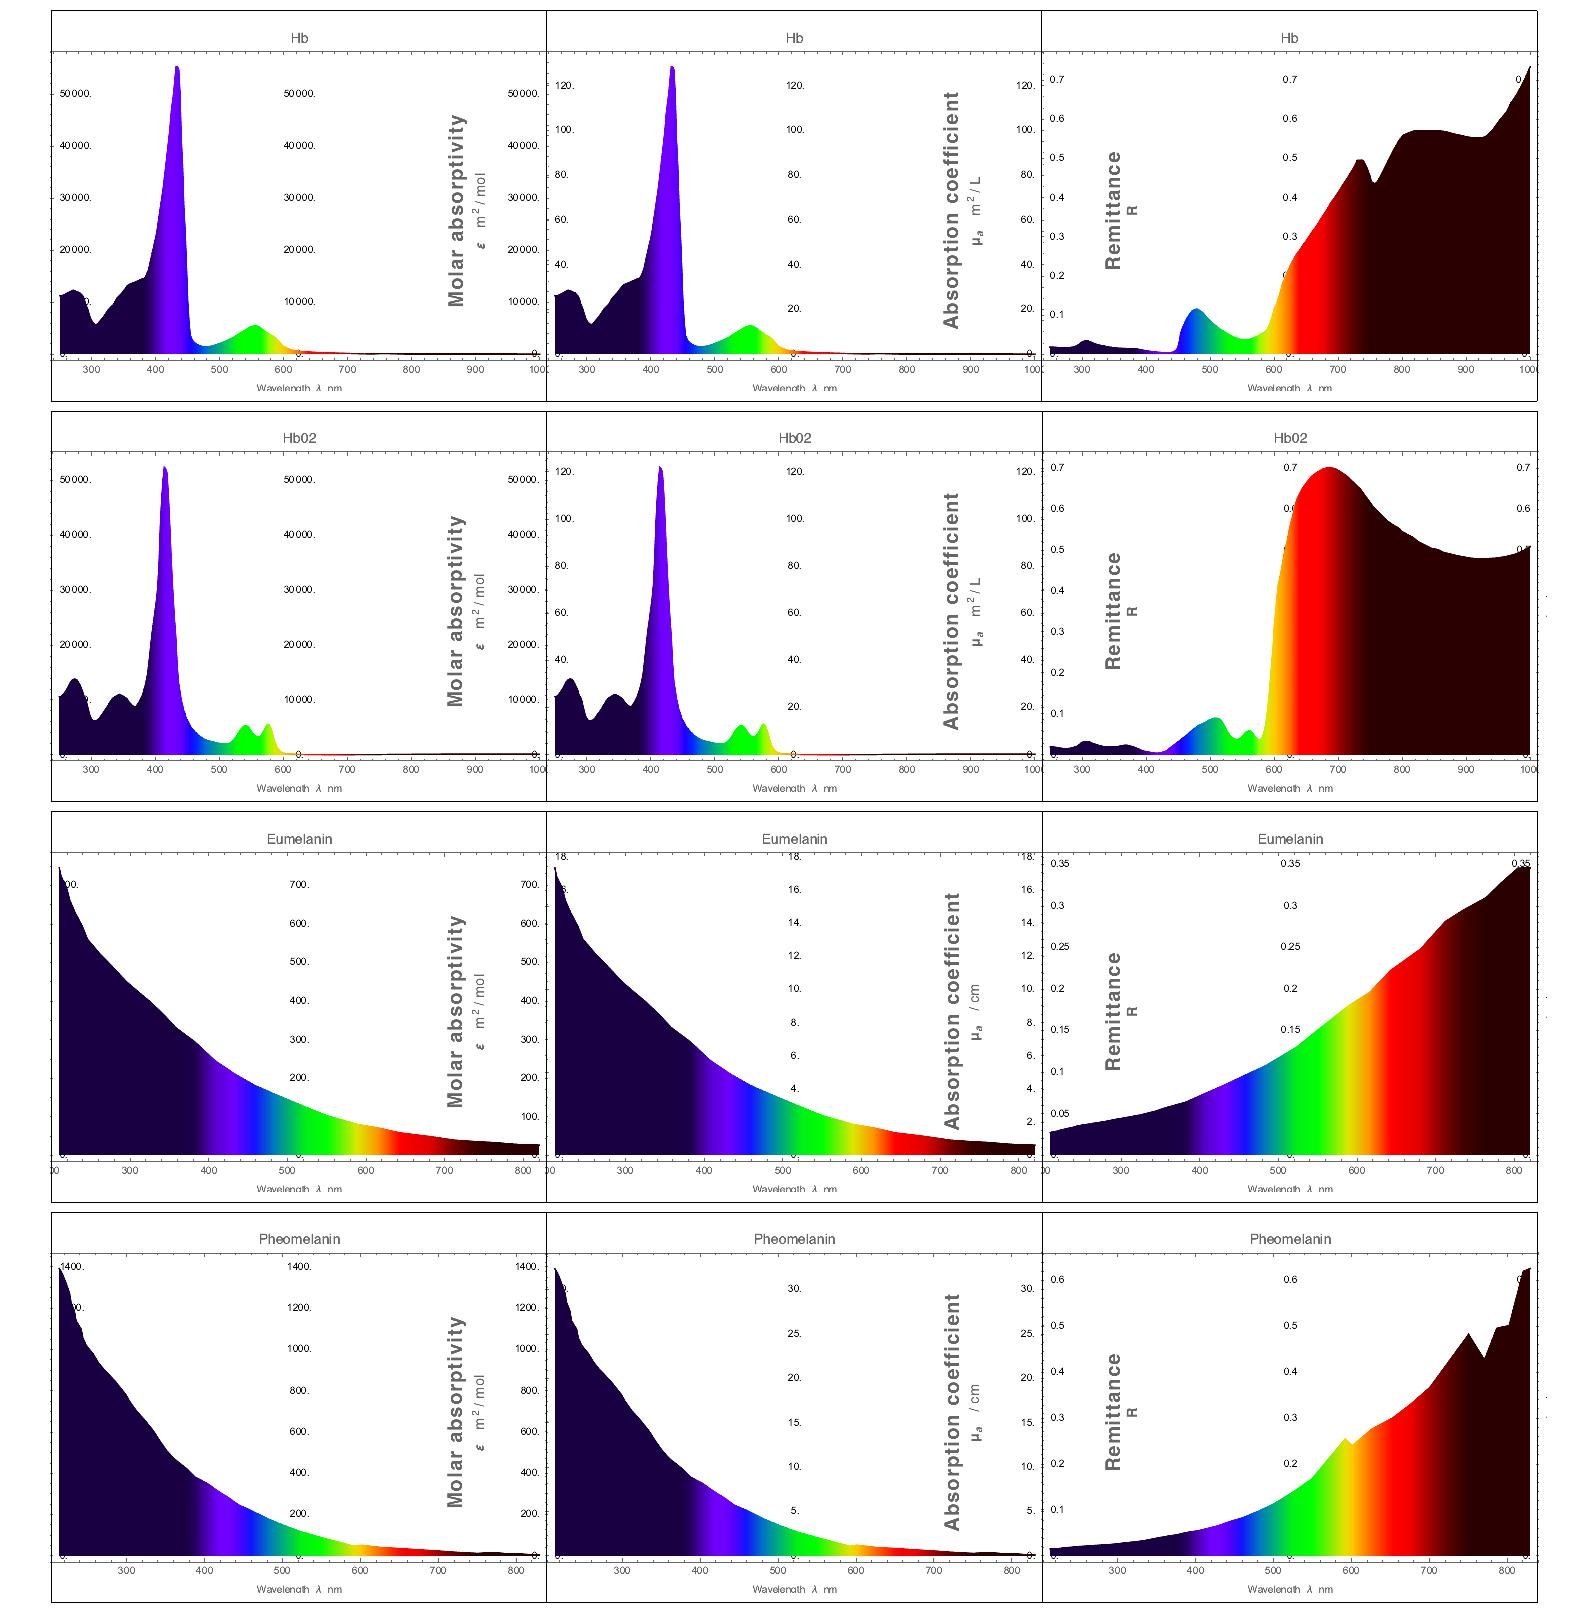
\includegraphics[width=0.99\textwidth]{Chapter1/Figs/ChemicalSpectralProperties.jpg}
    \caption{From left to right, the molar absorptivity, the absorption coefficient, and remittance of the four key chromophores. We assume a typical hemoglobin concentration of 150 $g/L$. The remittance was found using Kubelka-Munk Theory, outlined in section \ref{sec:SkinColorSimulation}. }  \label{fig:ChemicalSpectralProperties}
\end{figure}

The remittance spectra for the four key chromophores is shown in Figure \ref{fig:ChemicalSpectralProperties}. 

\subsection{Response Spectra}

The response spectrum is how a given sensor responds to specific wavelengths of light. Essentially, it is the raw output from the sensor, which is almost never used and is generally inaccessible even at the hardware layer, as the circuitry very close to the CCD does a basic level of color rebalancing. As we don't know the color rebalancing for every possible CCD, we observed the raw output spectra of several different devices and then tried two very simple methods of rebalancing the color:

The first is peak normalization, which simply levels out the maximum output in each channel such that the peak output for each of the channels is equal. This approach is very simple, and is quite likely from an electrical engineering perspective as it facilitates the digitization of the color information.

The second method is to approach the response spectra using basis functions to represent the spectrum. Using this approach, each basis function is normalized according to its integral over the visible wavelengths, giving an equal weighting to each of the response spectra functions over the range of values, rather than focusing on a peak value. Mathematically speaking, this approach is not unusual when constructing a basis set as it facilitates the maths.

It should be noted that the color rebalancing methods used in modern CCD devices are much more sophisticated than either of these approaches.

However, because the methods chosen here are straightforward amplifications of each channel, they're likely to be used as a first step in color rebalancing at the hardware level in the device. While we are not concerned with device constructions, it is useful to know how these devices capture the color information if this algorithm is to be used diagnostically, as color rebalancing may introduce artefacts and distortions in the data.

Although we consider these sensors to be capturing information throughout the entire visible spectrum, what they are actually capturing varies quite significantly between devices, as shown in Figure \ref{fig:ResponseSpectraStripes}. Even a very simple color rebalancing can restore some normality to the spectrum, as shown in Figure \ref{fig:ResponseSpectraStripesNorm}. However, as these devices use the aforementioned color rebalancing algorithms to alter the image to look more sensible to human eyes, these differences aren't so apparent to us.

\clearpage

\begin{figure}[h!]
  \centering
    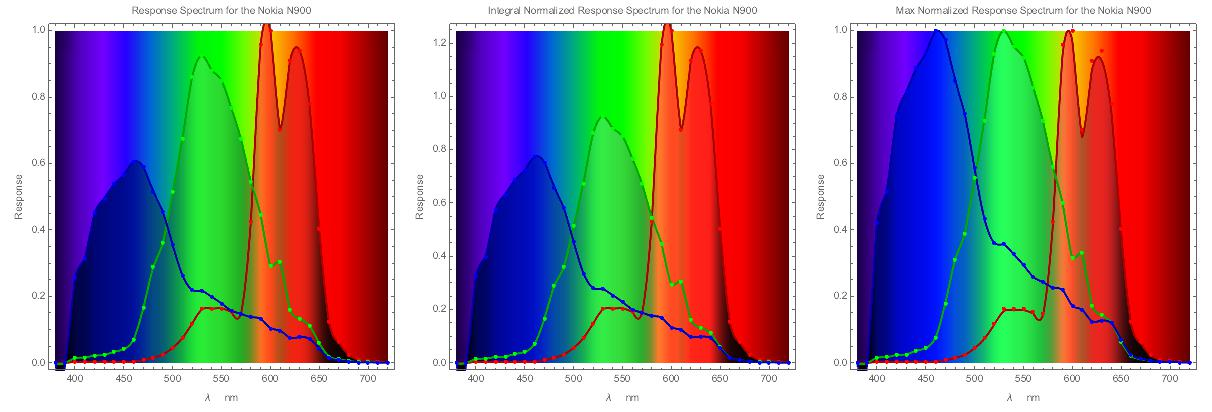
\includegraphics[width=0.99\textwidth]{Chapter1/Figs/ResponseSpectrum_NokiaN900.jpg}
    \caption{The response spectrum for the Nokia N900. }  \label{fig:ResponseSpectumNokia}
\end{figure}

\begin{figure}[h!]
  \centering
    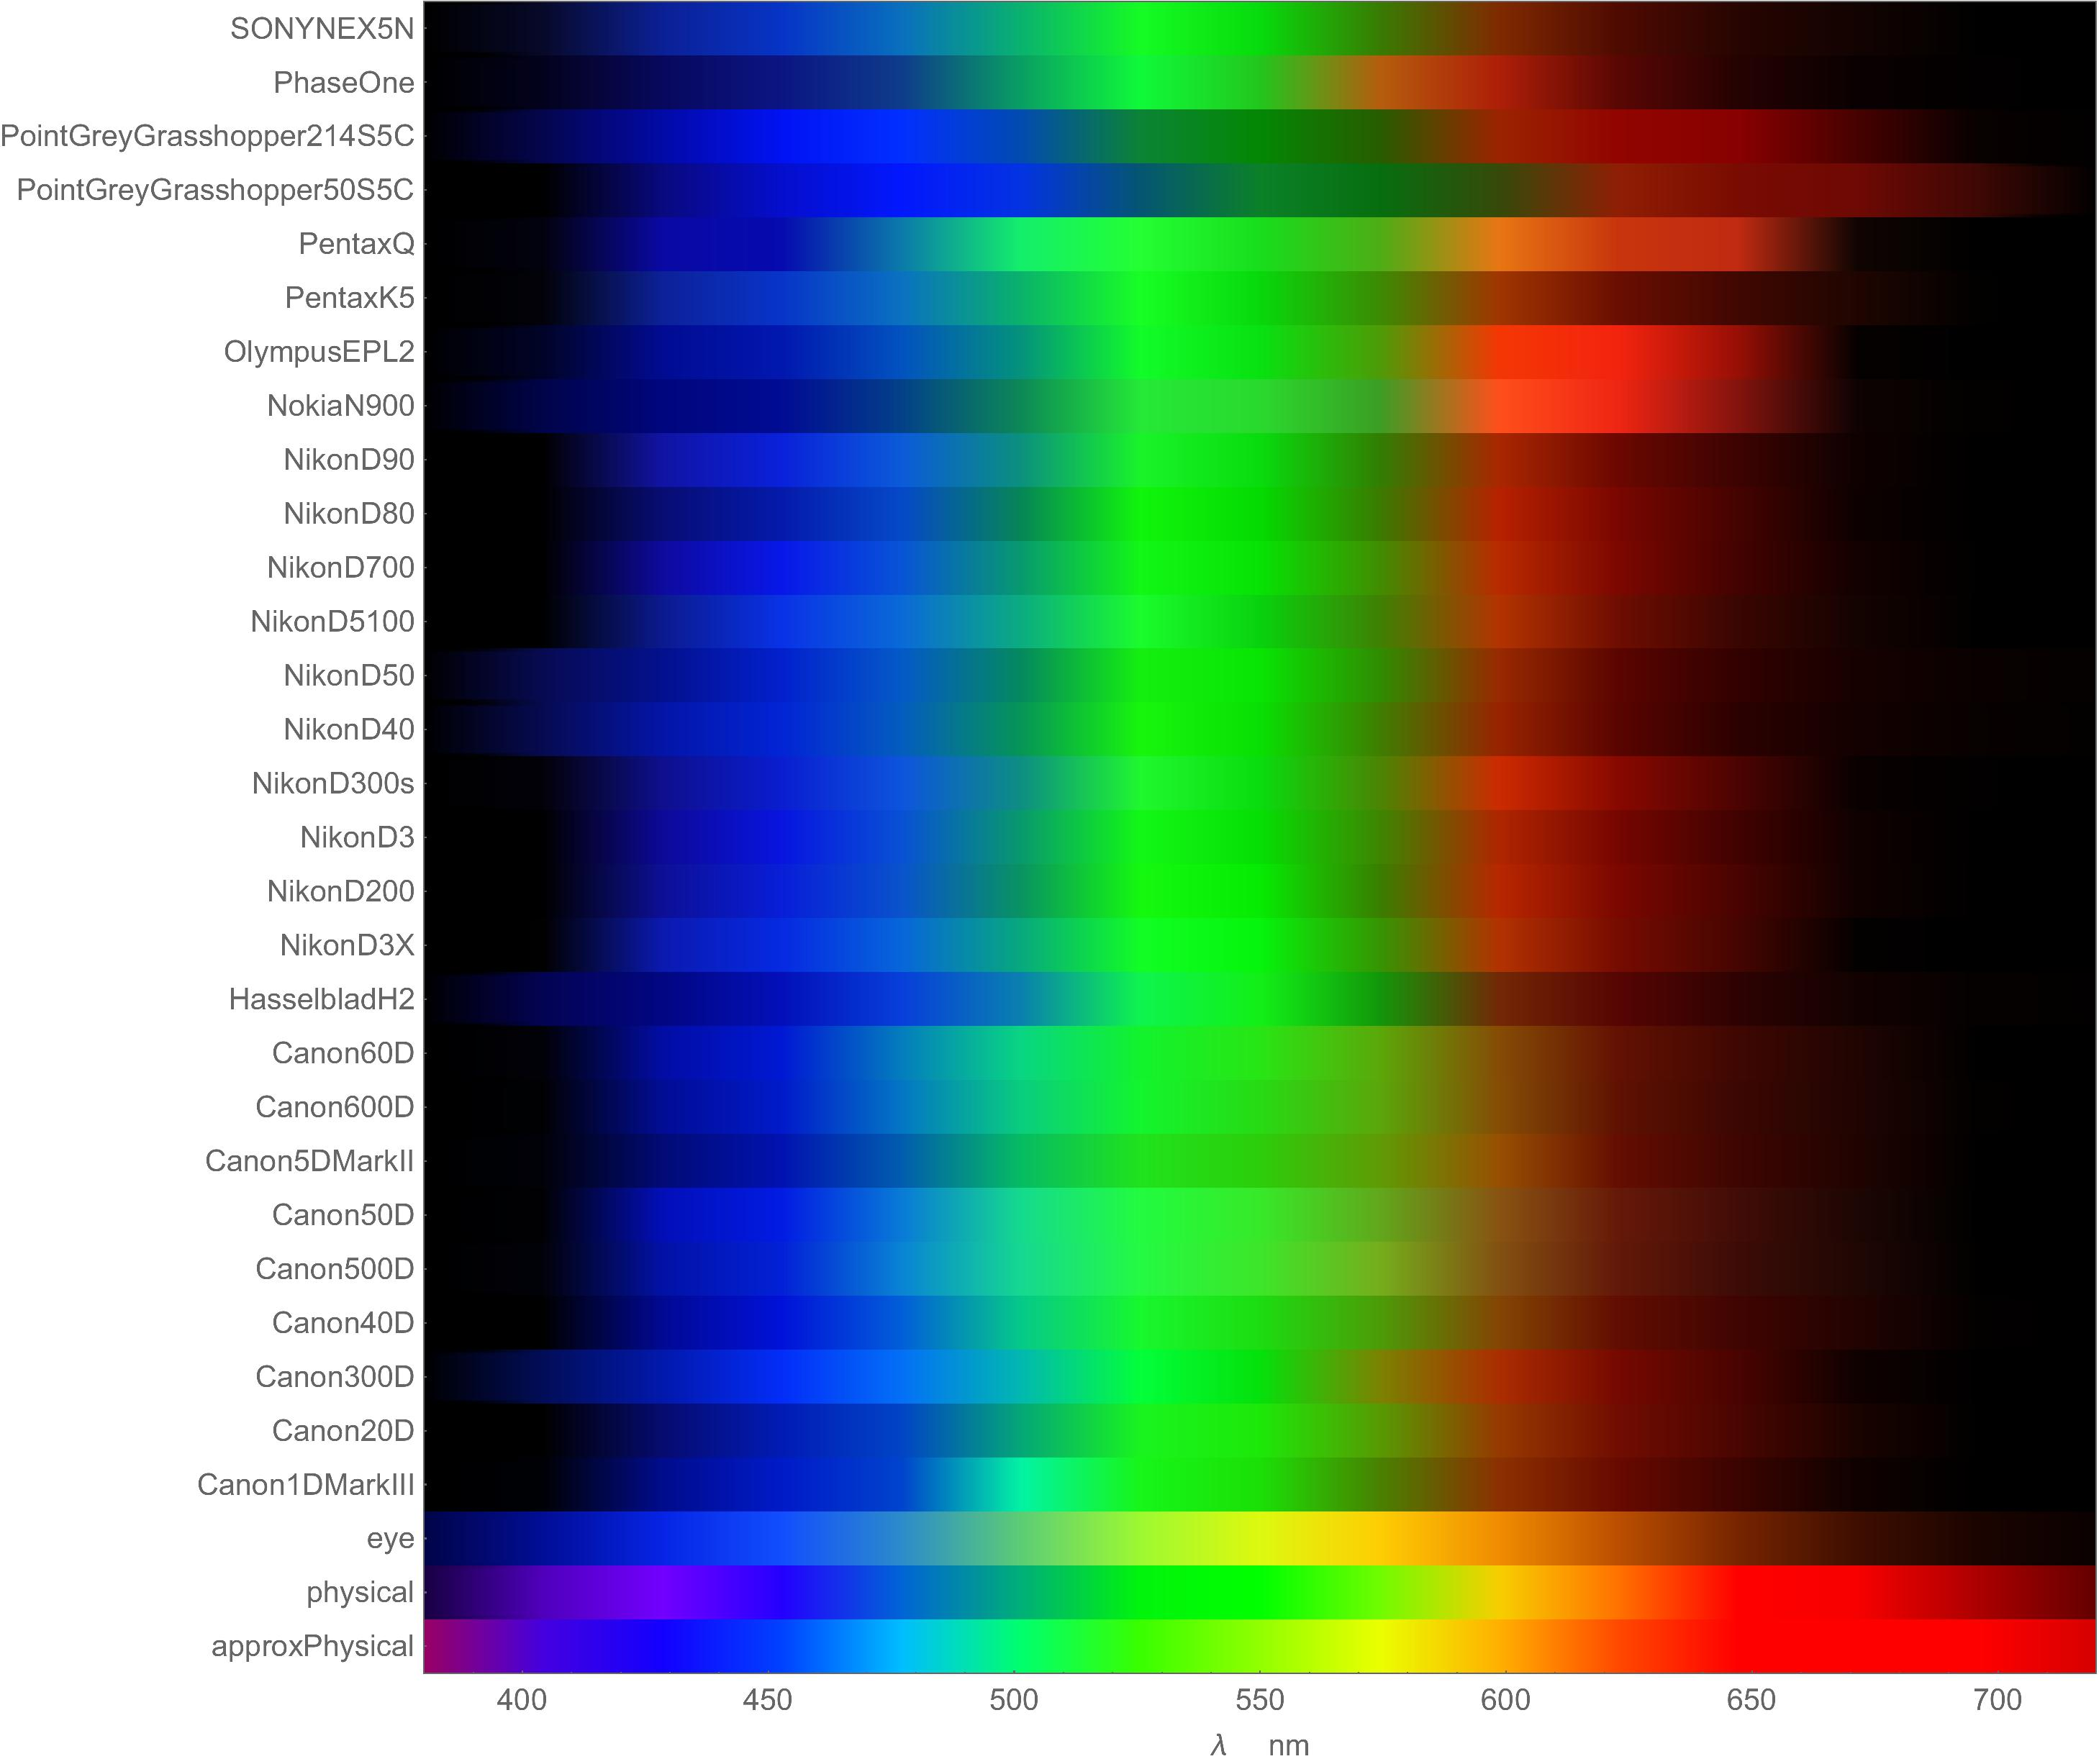
\includegraphics[width=0.99\textwidth]{Chapter1/Figs/ResponseSpectraStripes.jpg}
    \caption{The light spectrum as viewed using various CCDs with a physical spectrum for comparison.}  \label{fig:ResponseSpectraStripes}
\end{figure}

\clearpage

\begin{figure}[h!]
  \centering
    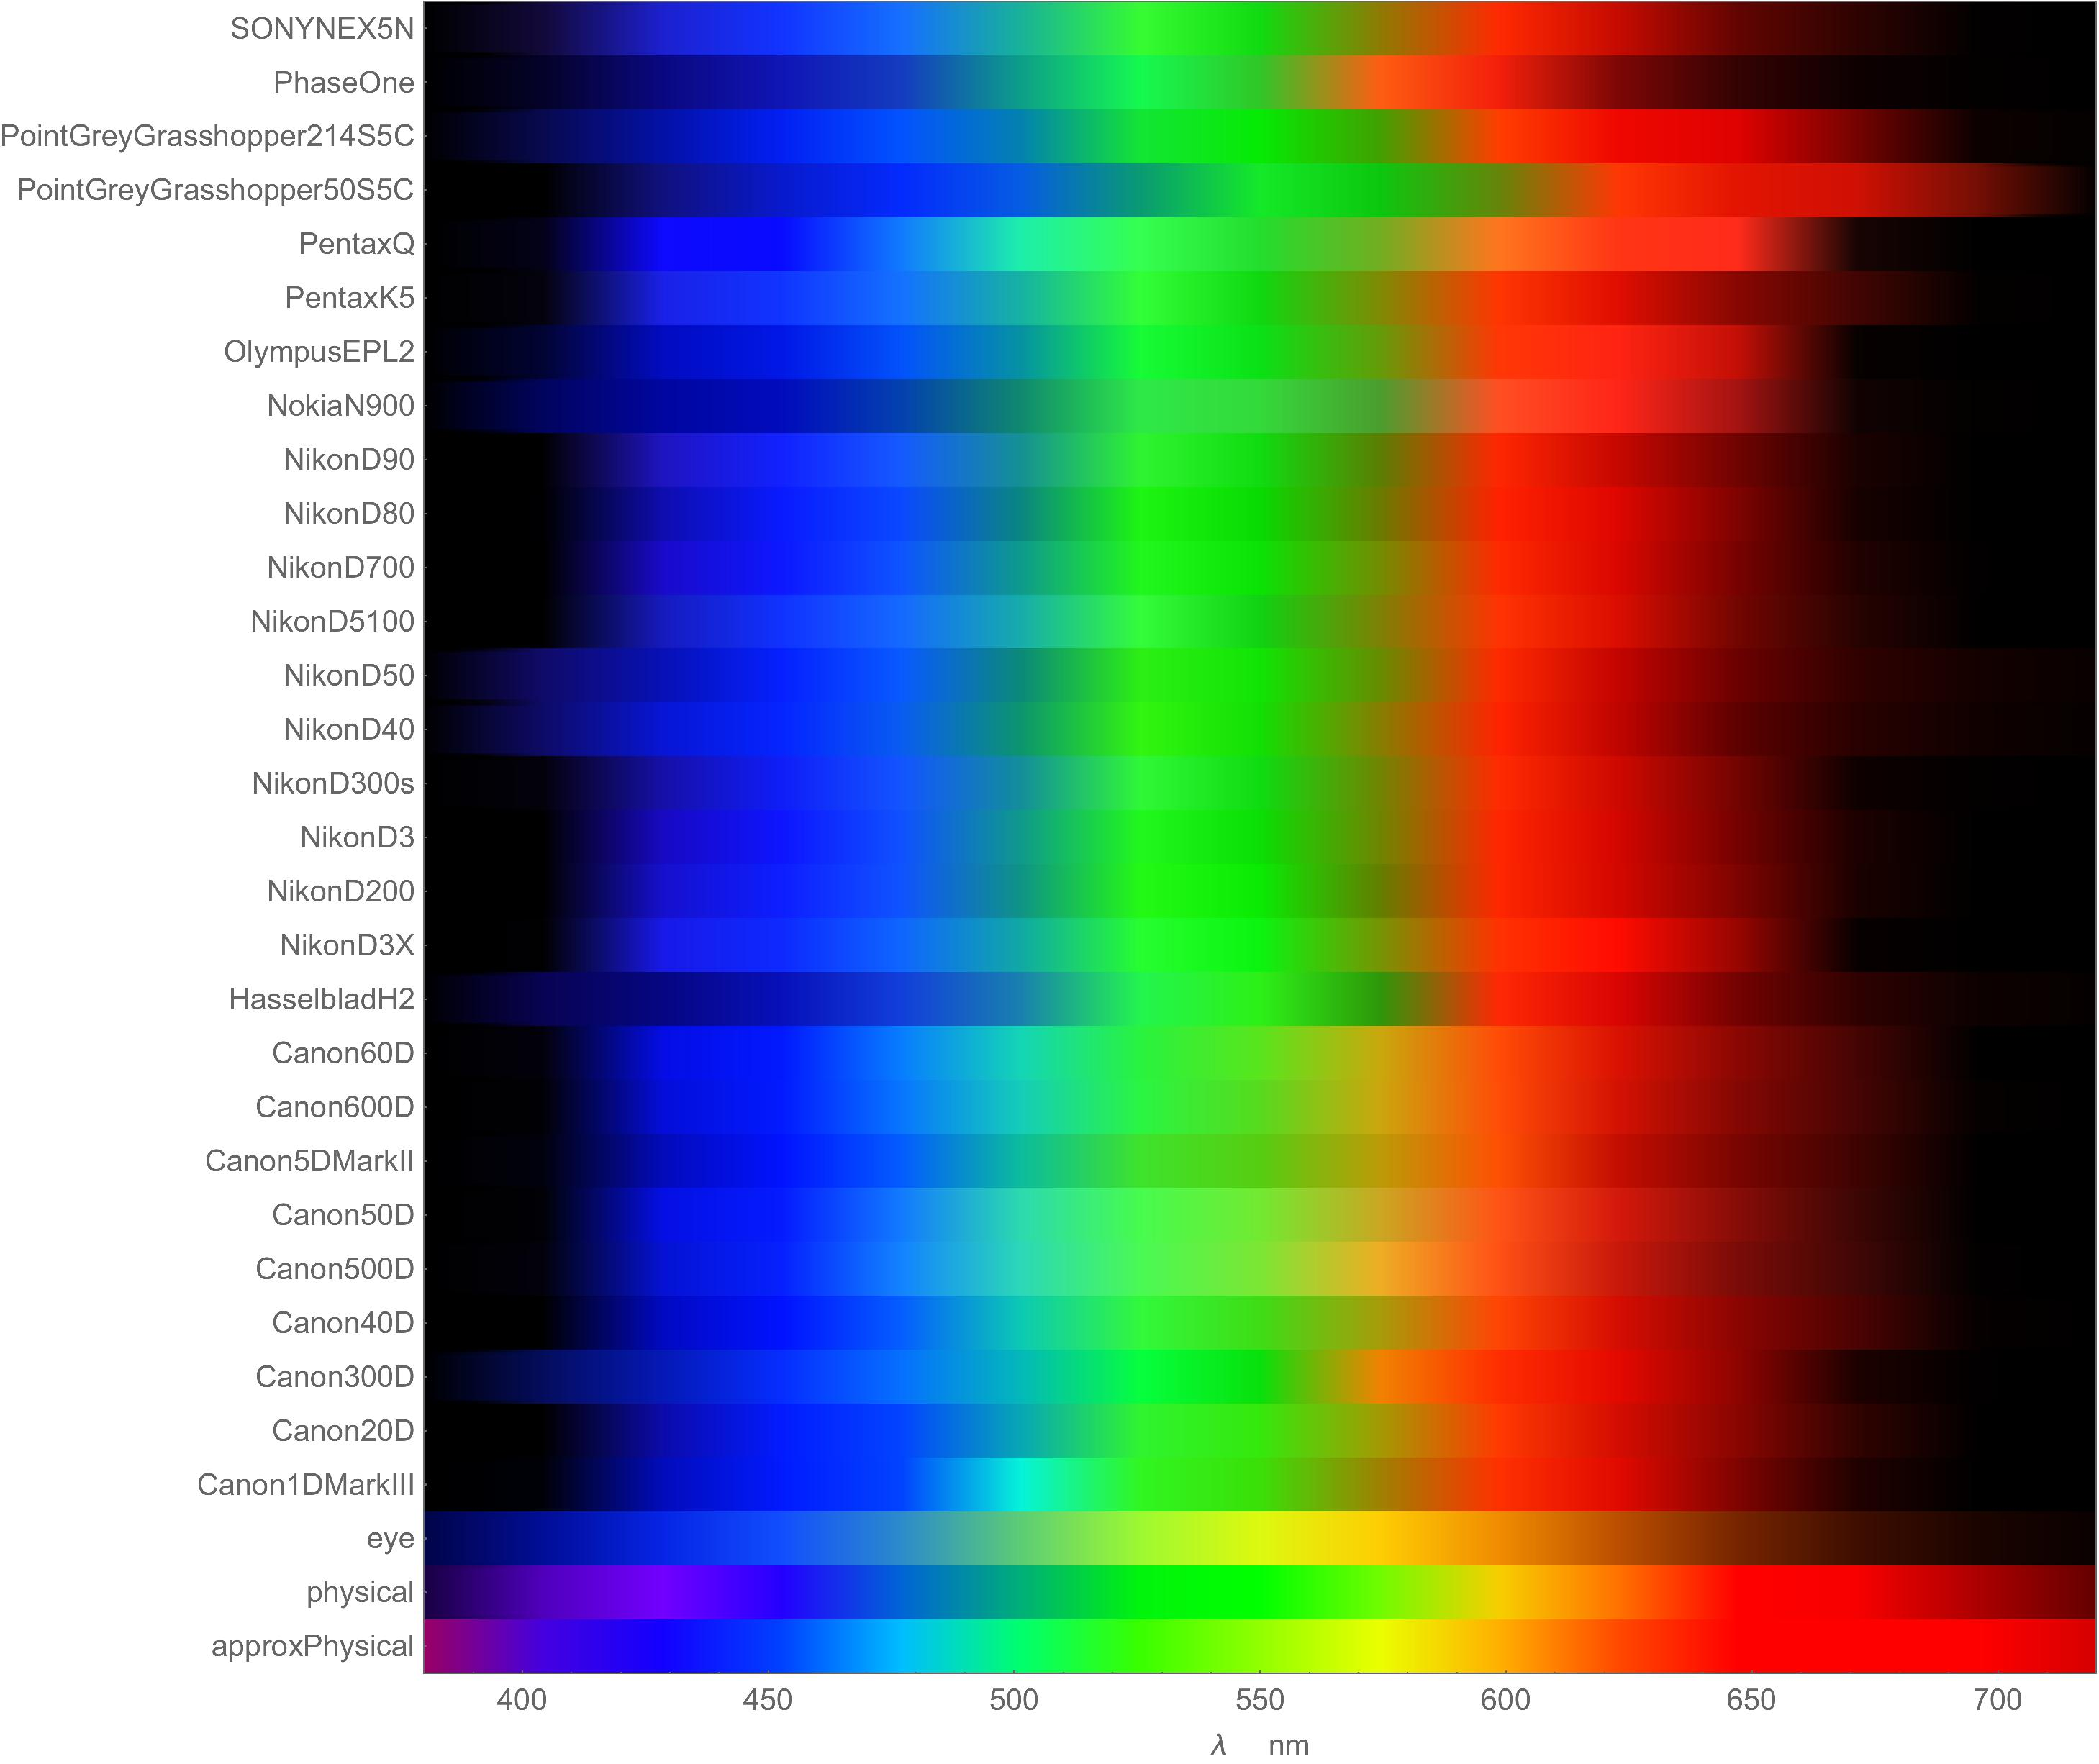
\includegraphics[width=0.99\textwidth]{Chapter1/Figs/ResponseSpectraStripesNorm.jpg}
    \caption{The light spectrum as viewed using various CCDs after normalization with a physical spectrum for comparison.}  \label{fig:ResponseSpectraStripesNorm}
\end{figure}

In addition to the color rebalancing, which corrects the behavior of the CCD devices, as is found in later sections, some devices, like the iPhone, also apply a dynamic color rebalancing which attempts to even out the colors based on the image captured. This feature is intended to correct for strange lighting conditions and other such problems which could affect the image. This will be addressed in detail in Chapter \ref{sec:Chap2}.

\clearpage

\subsection{Skin Color Simulation} \label{sec:SkinColorSimulation}

So, we have the molar absorptivity for the four key chromophores in the skin, we have the response spectra for a variety of devices, and a response spectra which serves as a target color output for all the devices after the color correction has been applied. Additionally, we are using the CIE 1931 RGB color-space for the absorption spectra, which is closer to how our eyes perceive color than any other color-space (\cite{RIDI2013}). This means that, in principle, we can get appropriate RGB values for the four key chromophores at the hardware layer using the device response spectra, or at the AP layer using the CIE 1931 RGB color-space spectrum, assuming the device's color-space correction does its job. The question now is how to actually simulate skin color.

Given a remittance spectrum $R(\lambda)$ and a response function $S_{rgb}(\lambda)$ for the sensor, the RGB output values can be calculated by finding the convolution 

\begin{align}
R & = \int_{0}^{\infty} R(\lambda) S_{R} (\lambda)  \mathbf{d\lambda}\\
G & = \int_{0}^{\infty} R(\lambda) S_{G} (\lambda) \mathbf{d\lambda}\\
B & = \int_{0}^{\infty} R(\lambda) S_{B} (\lambda)  \mathbf{d\lambda}
\end{align}

As for finding the RGB values, the bright color is the response of the CCD. By integrating the following functions in the figure below, we get the channel output seen in Figure~\ref{fig:Chromophores_NokiaN900}.


\begin{figure}[h!]
  \centering
    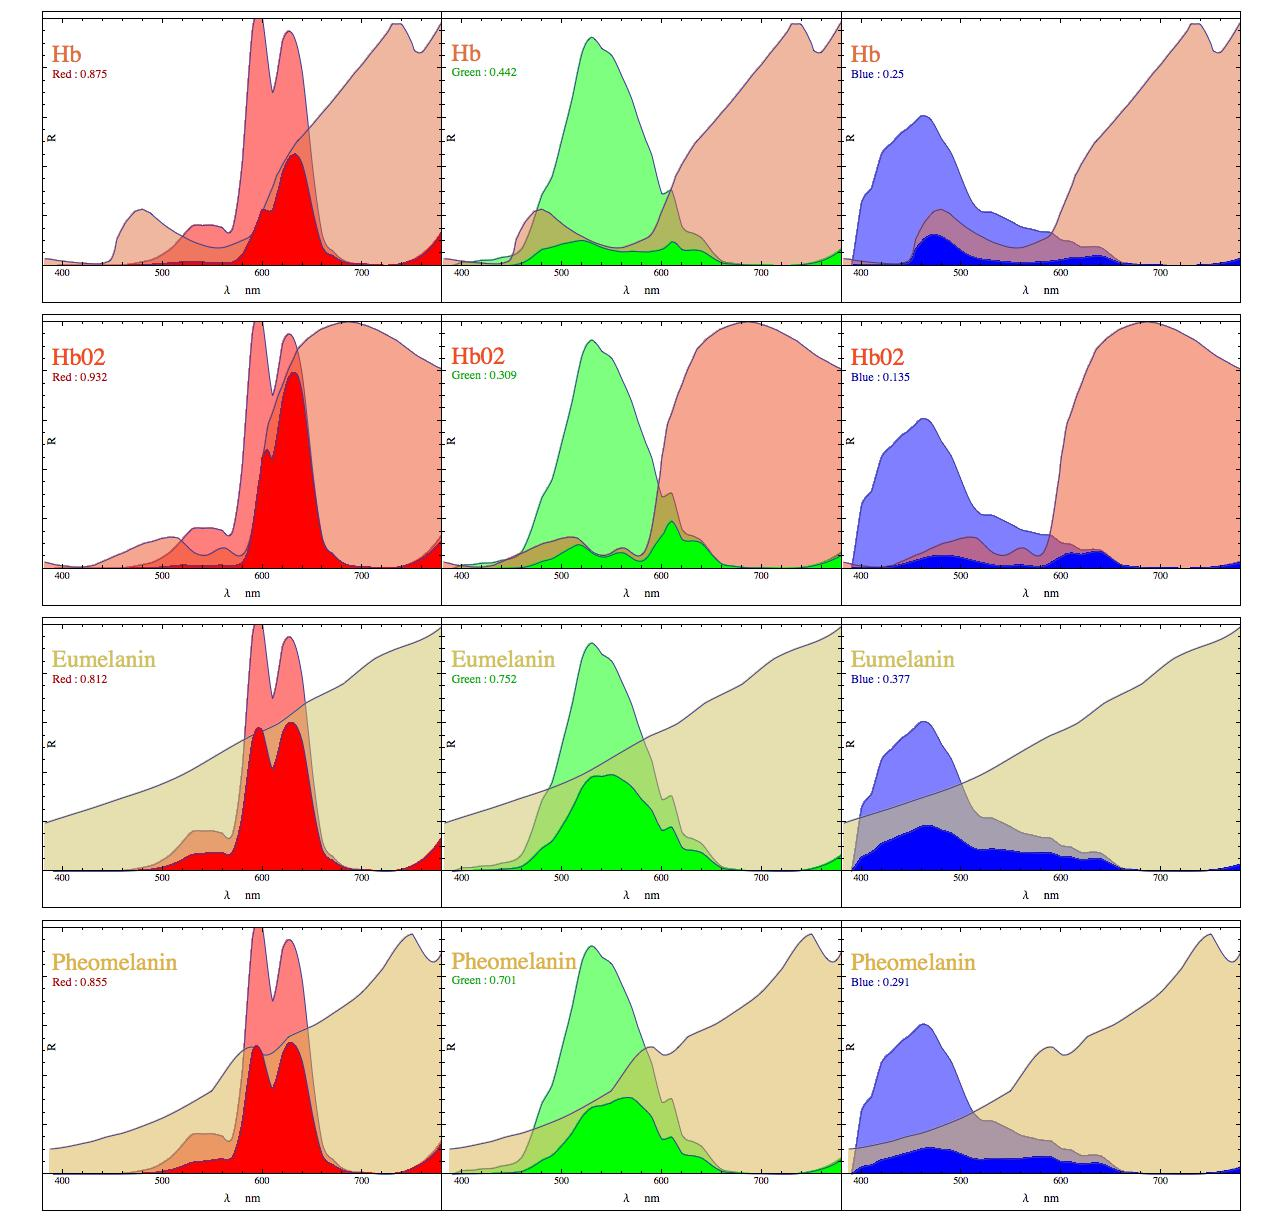
\includegraphics[width=0.99\textwidth]{Chapter1/Figs/Chromophores_NokiaN900.jpg}
    \caption{The functions representing the channel output of the four chromophores. The color of the remittance curve is the color for that particular chromophore as seen by the NokiaN900 camera. The solid-filled, bright function is the response of the CCD for each of the channels to that limited light, and the pale function is the response function of the CCD for each of the channels.}  \label{fig:Chromophores_NokiaN900}
\end{figure}



Thus, we can now find the channel output of any device for which we have a response function (Figure \ref{fig:CameraComparison}).

At the time of development, access to the camera on the iPhone was limited to the AP layer, and so we work with the CIE 1931 RGB color-space. The relative position of the chromophores in the color-space, is shown in Figure \ref{fig:ChromophoresYAB}.



%********************************** %First Section  **************************************
%\section{Motivation} %Section - 1.1 





%********************************** %Second Section  *************************************
%\section{Overview of Color Spaces} %Section - 1.2


%********************************** % Third Section  *************************************
%\section{Where does it come from?}  %Section - 1.3 
%\label{section1.3}


\begin{figure}[h!] %hi-res
  \centering
    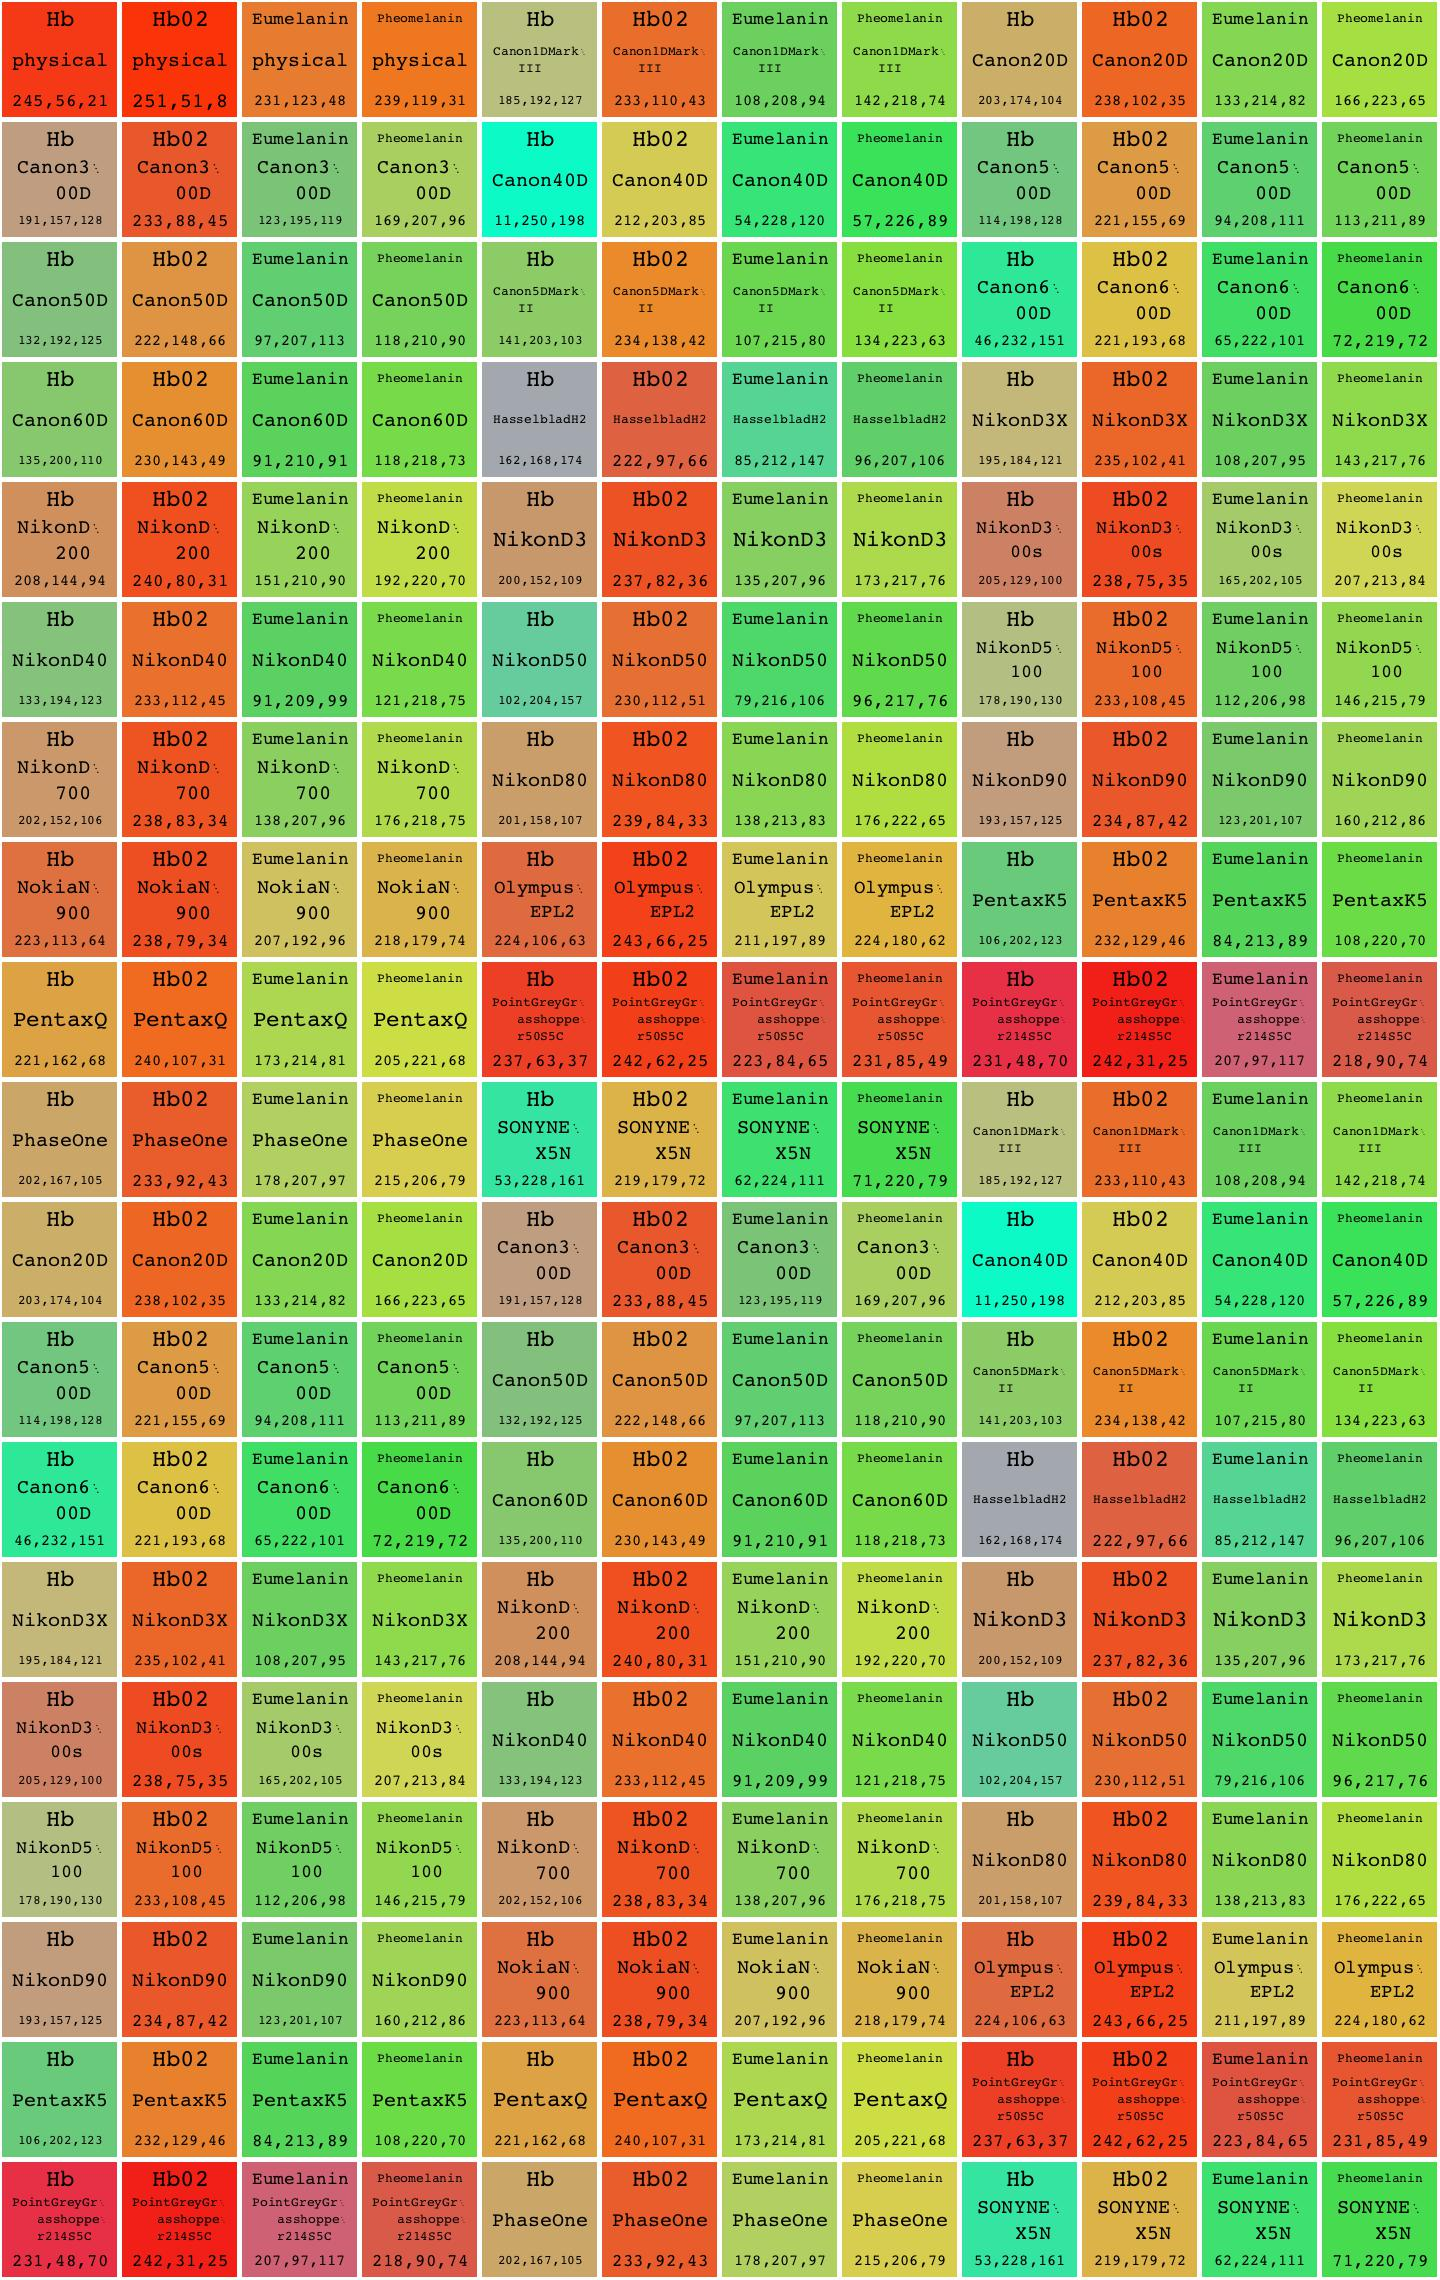
\includegraphics[width=0.99\textwidth]{Chapter1/Figs/CameraComparison.jpg}
    \caption{Chromophore colors as perceived by a range of devices.}  \label{fig:CameraComparison}
\end{figure}

\begin{figure}[h!]
  \centering
    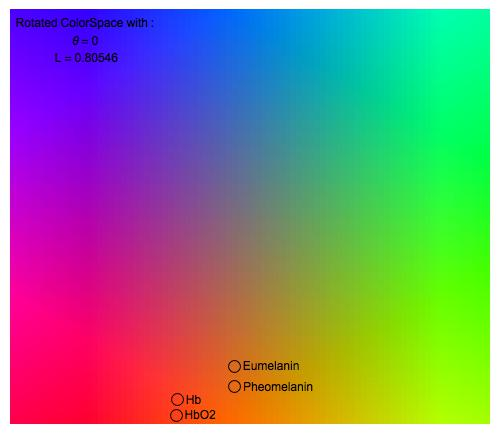
\includegraphics[width=0.99\textwidth]{Chapter1/Figs/ChromophoresYAB.jpg}
    \caption{The four main chromophores as perceived by CIE 1931 RGB color-space after rotation into the LCaCb $\theta = 0$ color-space.}  \label{fig:ChromophoresYAB}
\end{figure}
%*****************************************************************************************
%*********************************** Second Chapter **************************************
%*****************************************************************************************


\chapter{Color Spaces and Information Storage for Computer Vision Processing} \label{sec:Chap2}

\epstopdfsetup{outdir=Chapter2/Figs/PDF/}
\ifpdf
    \graphicspath{{Chapter2/Figs/Raster/}{Chapter2/Figs/PDF/}{Chapter2/Figs/}}
\else
    \graphicspath{{Chapter2/Figs/Vector/}{Chapter2/Figs/}}
\fi


\section{Constructing a New Color Space}\label{sec:ConstructingANewColorSpace}

In order to construct a new color-space, we need to consider the coordinate system, the orientation, and the fidelity of the discrete representation of the axes.

A Cartesian coordinate system allows for a straightforward transformation from the RGB source involving only rotation, translation and scaling. An orientation with a luminosity axis is useful because we're interested in the color information in the image. This choice determines two of three rotational degrees of freedom, as will be discussed below.

As for the discrete representation of the axes, it's desired that all the information captured pertaining to skin color should be preserved.

\subsection{Camera RGB and Normalization for Discrete Range}\label{sec:CameraRGB}

Due to the iPhone hardware being locked down at the application level, we do not have access to the raw camera feed. We do, however, have access to the post-processing (color-rebalanced and white-point-corrected) 8-bit RGB image data. Investigating the difficulties introduced by these processing effects and accounting for them is looked at in Chapter  \ref{sec:iPhoneCameraCharacteristics}.

Computer vision tasks are computationally intensive and often operate in real time. Reduction of the image data set size is a simple method for improving performance. There is, therefore, a need to develop techniques which keep the relevant information while quickly and efficiently discarding the irrelevant information. Achieving this for the RGB space is the aim of this chapter.

\section{The Skin Color Space Algorithm}

Appendix A outlines how an integer rotation matrix can be found and Appendix B describes how the rotated pixel values can be redistributed preserving all the chromatic information in a particular region. We can use these methods to build a color-space transformation algorithm which can make intelligent decisions about the numerical precision for the intermediate and final variables, as well as determining the most efficient transformation methods. The algorithm described herein will take values of $\theta$, the rotation about the luminosity axis, the standard deviations $ \uSTD{a}$,$ \uSTD{b}$ and mean values $ \uMean{a}$,$ \uMean{b}$ for the two chromatic axes in the unit range  and will automatically decide upon the necessary intermediate working data types and the most efficient re-distribution methods.

We found a rotational transformation which allows a working type $\tRange$ to be chosen such that $\tRange \le 2 \srcRange$ (Appendices \ref{app:AnIntegerRotationMatrix} and \ref{app:PreservationOfColorInformation}, where $\srcRange$ is the source type. If we were to keep the same data type $\dstRange$ for the color-space destination type as is used for the RGB values' source type $\srcRange$, then the axes would have to be rescaled with the accompanying loss of information. Given that we have values which allow us to assess where all the relevant information lies, a more sophisticated approach is possible. For a chromatic axis --- which, after rotation, has a length $L(\theta)$ --- we can determine the positions on that axis at which the information is considered irrelevant using Equation~(\ref{eq:LowHigh}) and the positions where the information is all considered relevant. If the gradient $ \Delta$ (\ref{eq:gradient}) is less than 1, then the distribution loses information at all points on the axis and the axis can be shortened without loss of relevant information. The only further consideration is to ensure that the values outside that range are prevented from causing errors associated with overflow. To exclude this possibility, a conditional statement can be used which checks the bounds as stated, assigning an appropriate value as necessary. The alternative is to use an intermediate value with a higher bit depth, and then to recast into the destination data type in such a way that overflow and underflow are handled appropriately. The OpenCV library provides a casting method --- "saturateCast" --- which serves this purpose.

\subsection{Setting the Value for the Tolerance}
Now that we have the working type range $\tRange$, accounting for both the rotation and the statistics, we can set a meaningful tolerance on the error. Previously, we calculated that the maximum error would occur for pixel values at the corners of the RGB cube; we have now seen that some values are more important than others and that it is more meaningful to use a smaller RGB cube which encloses only the values of interest. This cube is found by taking the values for $\Discard$ as the corners in the rotated space and rotating back to the RGB space. As this only needs to be done once it can be performed using floats in the unit spaces, however the values of $\discard$ account for the discrete numerics in that they are calculated from the discrete values $\Discard$ using the new values for $\kappa$ and $\tRange$ (Equations \ref{eq:DistributionConstants} and \ref{eq:newCompressionRatio}), where $\kappa$ is the compression ratio . In order to perform the inverse rotation, the values must be shifted to compensate for the natural range of the rotation which is: $\{0:1,-\text{\textonehalf}:\text{\textonehalf},-\text{\textonehalf}:\text{\textonehalf}\}$. 

\begin{align}
\discard^{RGB}_2 &= \nR^{-1} \cdot \left( \discard_2 - \Rc
        \right) & \text{where} \quad \Rc=\begin{pmatrix}
                 0   \\
                 \frac{1}{2}    \\
                 \frac{1}{2}     \\
                \end{pmatrix} \\
&= \R^{T} \cdot \left( \nS \otimes \left( \discard_2 - \Rc
                \right) \right)  
\end{align}

Because rotations of any angle are allowed, the values for $\discard^{RGB}_1$ may be larger than those for $\discard^{RGB}_2$ in the RGB space. The values may also be outside the RGB cube, meaning that the values may have to be truncated to fit inside the RGB cube range. 

The perturbation to the rotated channel elements $\dW$ (Equation \ref{eq:thePerturbationToTheRotatedChannelElements}) is found for an input set of pixel values $\discard^{RGB}_2$

\begin{align*}
\dW    &=  \min\left\{K \delta(\mu,\sigma) \right. ,  \left. \mathbf{L}(\theta) \right\} 
 \otimes 
        \begin{pmatrix}  0   \\   2   \\  2    \\ \end{pmatrix} 
  \otimes
        \dqEO\left[   \begin{pmatrix}  0   \\ \dqRe[ \thetaA ]  \\ \dqRe[ \Pii{6} -\thetaA]   \\ \end{pmatrix}  \right]
 \otimes
        \left( \dqs[\theta]  \cdot \discard^{RGB}_2 \right) 
\end{align*}

We have previously solved the case where both channels are of equal importance; we now need to find the values of $\alpha$ and $\beta$ which set the relative importance of each channel. There are two factors here: the channel scaling and the new, smaller RGB cube corners. The values for these also need to be put in correct correspondence with the $a$ and $b$ channel functions. For the scaling this is found by:

\begin{align*}
 \begin{pmatrix}  0   \\   \alpha_1   \\  \beta_1   \\ \end{pmatrix}     &=  
\dqEO\left[  \min\left\{K \delta(\mu,\sigma) \right. ,  \left. \mathbf{L}(\theta) \right\} 
 \otimes 
        \begin{pmatrix}  0   \\   2   \\  2    \\ \end{pmatrix} \right]
\end{align*}
For the new RGB corners we need to find the largest element which can result from the inner product with $\dqs[\theta]$. As the elements of $\dqs[\theta]$ are in $\{-1,0,1\}$, with only one occurrence of each in the second and third rows, we need to find the largest element of $\discard^{RGB}_2$ which is not in the zero position. The algorithm solves:

\begin{align*}
 \begin{pmatrix}  0   \\   \alpha_2   \\  \beta_2   \\ \end{pmatrix}     &=  
\dqEO\left[  
\max \left\{\text{abs}(\dqs[\theta]) \otimes \left(\discard^{RGB}_2 \right)^T \right\}
\right]
\end{align*}
where $\text{max}$ acts on each row and $\text{abs}(\dqs[\theta])  = \dqs[\theta] \otimes \dqs[\theta]$. 
These then give a combined value for $\alpha = \alpha_1 \alpha_2$ and $\beta = \beta_1 \beta_2$. Because the axes have been scaled so that the information on the axis is to be kept, at least, near the mean, the tolerance should be set to $\tau =1$. The condition for accepting a value of $\theta$ is $1 > h(i,\iota; \alpha,\beta)$.

\subsection{The Complete Algorithm}


The programmer specifies a requested value of $\theta$, values for the means $\uMean{{ab}}$ and standard deviations $\uSTD{ {ab}}$ for each of the three axes in the rotated color-space with a unit range and the data type ranges $\srcRange$ and $\dstRange$. The algorithm then proceeds as follows:
\newline
\algosection{Find the working type and range.} 
Using the distribution constants (\ref{eq:DistributionConstants}), the gradient at the mean in the unit range (\ref{eq:gradient}), and the natural rotated axis lengths (\ref{eq:L}):

%\begin{tabular}{|c|c|c|c|}
%\hline  \LaTeX & Mathematica & MatLab & C++ \\ 
%\hline  &  &  &  \\ 
%\hline  &  &  &  \\ 
%\hline  &  &  &  \\ 
%\hline  &  &  &  \\ 
%\hline  &  &  &  \\ 
%\hline  &  &  &  \\ 
%\hline  &  &  &  \\ 
%\hline  &  &  &  \\ 
%\hline 
%\end{tabular} 

\begin{gather*}
 \begin{aligned}
  \delta  &= \frac{ \sqrt{2} }{ \sigma \sqrt{\pi }  \left(\Sigma^+-\Sigma^-\right)} & 
 K & =  \frac{\dstRange}{\srcRange}  & 
 \Sigma^- &= \text{erf}\left(\frac{\mu -1}{\sqrt{2} \sigma }\right) &
 \Sigma^+ &= \text{erf}\left(\frac{\mu }{\sqrt{2} \sigma }\right) 
  \end{aligned} \\
  \mathbf{L}(\theta) =
  \begin{pmatrix}
  \sqrt{3} \\
   \sqrt{\frac{2}{3}} \sin \left(\widetilde{\vartheta}\right) + \sqrt{2} \cos \left(\widetilde{\vartheta}\right) \\  
  \sqrt{\frac{2}{3}} \sin \left(\widetilde{\theta}\right) + \sqrt{2} \cos \left(\widetilde{\theta}\right) 
  \end{pmatrix}
  \quad \text{where}  \quad 
  \begin{array}{c}
  \widetilde{\vartheta} = \left(\theta - \Pii{6}\right) \bmod \frac{\pi }{3} \\
  \widetilde{\theta} = \theta  \bmod \frac{\pi }{3} 
  \end{array}
\end{gather*}
The length of the axis $\tRange$ after rescaling is given by Equation \ref{eq:CombinedRotationRange}, and the axis limits are easily found along with 
the compression ratio $\kappa$ (Equation \ref{eq:newCompressionRatio}).
\begin{gather*}
\begin{aligned}
 \tRange(\theta,\mu,\sigma)   & =  \min\left\{K \delta(\mu,\sigma) \right. ,  \left. \mathbf{L}(\theta) \right\}  \srcRange \quad&\quad
 \kappa(\theta) & = \max\left\{ \frac{1}{\delta(\mu,\sigma) }   , \frac{K}{\mathbf{L}(\theta)} \right\}  
 \end{aligned} \\
 \begin{aligned}
  \tMin(\theta,\mu,\sigma)   & =
 \begin{pmatrix}
 0 \\
  \frac{-1 }{2} \tRange_2(\theta,\mu_2,\sigma_2) \\  
  \frac{-1 }{2} \tRange_3(\theta,\mu_3,\sigma_3) \\  
 \end{pmatrix} \quad & \quad
  \tMax(\theta,\mu,\sigma)   & =
 \begin{pmatrix}
  \tRange_1(\theta,\mu_1,\sigma_1)  \\
  \frac{1 }{2} \tRange_2(\theta,\mu_2,\sigma_2)  \\  
  \frac{1 }{2} \tRange_3(\theta,\mu_3,\sigma_3)  \\  
 \end{pmatrix} 
 \end{aligned}
\end{gather*}


\algosection{Set the distribution region boundary constants.} 
Using the constants defined in Equations \ref{eq:PreservedRegionConsts} and \ref{eq:0to1}
\begin{align*}
  w(\mu,\sigma)  & =  \sigma  \sqrt{ \log \left(\frac{2}{\pi } \right) -2 \log \left(\kappa \sigma  \left(\Sigma^+-\Sigma^-\right)\right) } &
  \text{dL} &= \frac{1}{\dstRange} 
\end{align*}
We find the boundaries in the unit range 
\begin{equation}
\begin{aligned}
\discard_1 &= \sigma \sqrt{2} \; \text{erf}^{-1}\left((\text{dL}-1) \Sigma^+-\text{dL} \; \Sigma^-\right)+\mu  &       
\keep_1(\mu,\sigma) &= \mu - w(\mu,\sigma)  \\     
\discard_2 &= \sigma \sqrt{2} \; \text{erf}^{-1}\left((\text{dL}-1) \Sigma^- -\text{dL} \; \Sigma^+ \right)+\mu &
\keep_2(\mu,\sigma) &= \mu + w(\mu,\sigma) 
\end{aligned}
\end{equation}
and the boundaries in the working range
\begin{equation}
\begin{aligned}
\Discard &= \tMin + \tRange \left( \discard(\mu,\sigma) \right) & 
\Keep(\mu,\sigma) &= \tMin + \tRange\left( \keep(\mu,\sigma) \right) 
\end{aligned}
\end{equation}
The extended region in which all the information is kept is found by numerically solving the defining equations for the  extended boundaries $\eKeep_1$ and $\eKeep_2$ with the practical introduction of a parameter $ \tau_{p} $, which extends the acceptable deviation from linearity. So $ \tau_{p} =1$ would allow 1 discarded piece of information within the extended region.
\begin{equation}
\begin{aligned}
\left\lceil\text{dis}\left(\Keep _1\right)\right\rceil-\Keep _1 - \tau_{p} & =\text{dis}\left(\eKeep _1\right)- \eKeep _1 &
\left\lfloor\text{dis}\left(\Keep _2\right)\right\rfloor-\Keep _2 - \tau_{p} & =\text{dis}\left(\eKeep _2\right)- \eKeep _2 
\end{aligned}
\end{equation}
The C++ code finds the points using the following algorithm

\begin{algorithm}[H]
\begin{algorithmic}
 \Require{$\Keep _2$ the starting point for the linear walk } 
 \linebreak \phantom{Require} $\tau_{p}$ the acceptable divergence from linearity 
 \Ensure{$ \{\eKeep_1, \eKeep_2\} $ the extended boundaries}
 \State $x \gets \Keep_2$  \Comment{$dis(x)$ is the distribution function}
 \While{$dis(x) > x + \left\lfloor\text{dis}\left(\Keep _2\right)\right\rfloor  -\Keep _2 - \tau_{p}$}
     \State  x++ 
 \EndWhile
 \State $\eKeep_2 \gets x$ 
 \State $\eKeep_1 \gets \Keep _1 - (\eKeep_2 - \Keep _2)$ \Comment{Exploiting a symetry dis(x)}
 \State \textbf{Return} {$\eKeep_1$ ,$\eKeep_2$ }
 \end{algorithmic}
  \caption{Finding the extended region in which all the information is kept in C++}
\end{algorithm}

The unit range boundaries $\ekeep$ are found using  $\ekeep =  \frac{\eKeep - \tMin}{\tRange}$.


\algosection{Suggest a new value for $\theta$.} 
First we find the perturbation scaling (\ref{eq:perturbationFunctionSigns}) and the perturbation function ordering function (\ref{eq:abPerturbationFunctionOrdering}).
\begin{gather}\label{eq:abPerturbationFunctionOrdering}
\dqEO[  \left(
\begin{smallmatrix}
 0   \\
 a   \\
 b  \\
 \end{smallmatrix} 
\right)  ,\theta ] =
\begin{cases}
 \left(
\begin{smallmatrix}
 0 \\
 a  \\
 b \\
\end{smallmatrix} 
\right) & 0\leq (\theta  \bmod \frac{\pi}{3} )<\frac{\pi }{6} \\
 \left(
\begin{smallmatrix}
 0 \\
 b  \\
 a \\
\end{smallmatrix} 
\right) & \frac{\pi }{6} \leq (\theta  \bmod \frac{\pi}{3} ) < \frac{\pi }{3} 
\end{cases} \\
\dqs[\theta] =
\begin{cases}
 \left(
\begin{smallmatrix}
 0 & 0 & 0 \\
 1 & 0 & -1 \\
 1 & -1 & 0 \\
\end{smallmatrix} 
\right) & 0\leq (\theta  \bmod \pi )<\frac{\pi }{6} \\
 \left(
\begin{smallmatrix}
 0 & 0 & 0 \\
 0 & 1 & -1 \\
 -1 & 1 & 0 \\
\end{smallmatrix} 
\right) & \frac{\pi }{6}\leq (\theta  \bmod \pi )<\frac{\pi }{3} \\
 \left(
\begin{smallmatrix}
 0 & 0 & 0 \\
 0 & -1 & 1 \\
 -1 & 0 & 1 \\
\end{smallmatrix} 
\right) & \frac{\pi }{3}\leq (\theta  \bmod \pi )<\frac{\pi }{2} \\
 \left(
\begin{smallmatrix}
 0 & 0 & 0 \\
 1 & -1 & 0 \\
 1 & 0 & -1 \\
\end{smallmatrix} 
\right) & \frac{\pi }{2}\leq (\theta  \bmod \pi )<\frac{2 \pi }{3} \\
 \left(
\begin{smallmatrix}
 0 & 0 & 0 \\
 -1 & 1 & 0 \\
 0 & 1 & -1 \\
\end{smallmatrix} 
\right) & \frac{2 \pi }{3}\leq (\theta  \bmod \pi )<\frac{5 \pi }{6} \\
 \left(
\begin{smallmatrix}
 0 & 0 & 0 \\
 -1 & 0 & 1 \\
 0 & -1 & 1 \\
\end{smallmatrix} 
\right) & \frac{5 \pi }{6}\leq (\theta  \bmod \pi )<\pi 
\end{cases}
\end{gather}
In order to set the values for the scaling of the perturbation $\alpha$ and $\beta$, the absolute value of the perturbation matrix sign $\left\lVert \dqs[\theta] \right\rVert$ can be written in terms of a single row vector function $\dqas[\theta]$ 
\begin{align*}
\left\lVert \dqs[\theta] \right\rVert & = 
\left( \begin{smallmatrix}  0&0&0   \\   \cdots & \dqas[\theta + \frac{\pi}{2}] & \cdots   \\  \cdots & \dqas[\theta]   & \cdots  \\ \end{smallmatrix}  \right) 
&
\dqas[\theta] &=\begin{cases}
\left(\begin{smallmatrix} 1 & 1 & 0 \end{smallmatrix} \right)&  0                     \leq \scalebox{0.75}{ $(\theta \bmod \pi )$ }<\frac{   \pi }{3} \\
\left(\begin{smallmatrix} 1 & 0 & 1 \end{smallmatrix} \right)&  \frac{   \pi }{3}\leq \scalebox{0.75}{ $(\theta \bmod \pi )$ }<\frac{2 \pi }{3} \\
\left(\begin{smallmatrix} 0 & 1 & 1 \end{smallmatrix} \right) & \frac{2 \pi }{3}\leq \scalebox{0.75}{ $(\theta \bmod \pi )$ }<\pi  \\
\end{cases} 
\end{align*}
Then we find the point at which loss of information does not matter in RGB space $\discard^{RGB}_2$ 
\begin{align*}
\discard^{RGB}_2 &= \max \left\{ 
  \R^{T} \cdot \left( \nS \otimes \left( \discard_1 - \Rc \right) \right) , 
  \R^{T} \cdot \left( \nS \otimes \left( \discard_2 - \Rc \right) \right) 
\right\} &
 \text{where} \quad \Rc=
\begin{pmatrix}
                 0   \\
                 \frac{1}{2}    \\
                 \frac{1}{2}     \\
\end{pmatrix} 
\end{align*}

Then we numerically find 

\begin{align*}
 \begin{pmatrix}  0   \\   \alpha   \\  \beta   \\ \end{pmatrix}     % &=  
%\dqEO\left[  \min\left\{K \delta(\mu,\sigma) \right. ,  \left. \mathbf{L}(\theta) \right\} 
% \otimes 
%        \begin{pmatrix}  0   \\   2   \\  2    \\ \end{pmatrix} 
%         \otimes 
%        \max \left\{\text{abs}(\dqs[\theta]) \otimes \left(\discard^{RGB}_2 \right)^T \right\}
%        \right]\\
        &=\dqEO\left[ \begin{pmatrix} 
         0 \\ 
         2 \min\left\{K \delta(\mu_2,\sigma_2) \right. ,  \left. \mathbf{L}_2(\theta) \right\}  \max \left\{\dqas[\theta + \frac{\pi}{2}]  \otimes \left(\discard^{RGB}_2 \right)^T \right\}  \\
         2 \min\left\{K \delta(\mu_3,\sigma_3) \right. ,  \left. \mathbf{L}_3(\theta) \right\}  \max \left\{\dqas[\theta                       ] \otimes \left(\discard^{RGB}_2 \right)^T \right\}   \\
          \end{pmatrix} \right]
\end{align*}

The algorithm then finds a starting value for the index (\ref{eq:indexFromTheta}) and returns the closest value which satisfies the tolerance (\ref{eq:generalizedPerturbation}):

%\setlength{\belowdisplayskip}{0pt} \setlength{\belowdisplayshortskip}{0pt}
%\setlength{\abovedisplayskip}{0pt} \setlength{\abovedisplayshortskip}{0pt}

\begin{align*}
 i(\delta\theta, n) &= \frac{\meanIndx \tan (\delta \theta ) \left(\sqrt{3} \tan (\delta \theta )+7\right)}{\tan (\delta \theta )+\sqrt{3}} &
  \delta\theta &= \theta \mod{\frac{\pi}{6} } &
  \meanIndx & = 2^{n-3} 
\end{align*}

The region $\iota$ for a given value of $i$ is found and the appropriate values (\ref{eq:extremaBounds}) for the extrema (\ref{eq:ExtremaFunctions}) are evaluated in the function which finds the perturbation at the index (\ref{eq:generalizedPerturbation}) and the intercept position $\thetaX{i}$ is found with algorithm \ref{algo:thetaX}.
%\begin{gather*}
%\begin{aligned}
% \iota(i,n)  &= \left\lfloor 7\ \meanIndx-\sqrt{i^2 - 2 i \; \meanIndx + 49\ \meanIndx^2 }\right\rfloor &
%  \extremaTheta{a} {l} = & \arctan\left(\frac{l \sqrt{3} }{2^n - l}\right) &
%  \extremaTheta{b} {l} = & \arctan\left(\frac{l \; 2^{2-n}}{\sqrt{3}}       \right)
%\end{aligned} \\
%\begin{aligned}
% \minimaTheta{a}  &= \extremaTheta{a}{i+\iota} &
% \maximaTheta{b} &= \extremaTheta{b}{i-\iota-1} & 
% \minimaTheta{b}  &= \extremaTheta{b}{i-\iota}  &
% \maximaTheta{a} &= \extremaTheta{a}{i+\iota+1}  &
%  \text{when} \quad 
%i + \iota &\in \{2 \mathbb{N}     \} \\
% \maximaTheta{a}  &= \extremaTheta{a}{i+\iota} & 
% \minimaTheta{b}  &= \extremaTheta{b} {i-\iota-1} &
% \maximaTheta{b} &= \extremaTheta{b}{i-\iota}  &
% \minimaTheta{a}  &= \extremaTheta{a}{i+\iota+1}  & 
%\text{when} \quad 
%i + \iota &\in \{2 \mathbb{N}  + 1 \} 
%\end{aligned}\\
%\thetaX{i} = \left\{\frac{
%\beta \minimaTheta{b} (\minimaTheta{a}  -\maximaTheta{a} )+\alpha  \minimaTheta{a} (\maximaTheta{b}-\minimaTheta{b})  }{
%\beta  (\minimaTheta{a} -\maximaTheta{a})+\alpha  (\maximaTheta{b}-\minimaTheta{b})
%},\frac{
%\alpha  \beta  (\minimaTheta{a}-\minimaTheta{b})  }{
%\beta  (\minimaTheta{a}-\maximaTheta{a})+\alpha  (\maximaTheta{b}-\minimaTheta{b})
%}\right\}
%\end{gather*}

 \begin{algorithm}[h]
 \begin{algorithmic}
      \Function { $\overset{\times}{\phi}$}{$ i, \alpha, \beta, n $} \Comment{$i$ integer index of the intercept }
       \State $\meanIndx \gets  2^{n-3}$  ; \quad  $\iota(i,n)  \gets  \left\lfloor 7\ \meanIndx-\sqrt{i^2 - 2 i \meanIndx + 49\ \meanIndx^2 }\right\rfloor $  \Comment{$n$ the source bit depth}
        \State $\extremaTheta{b}{\mathbf{l} } = \arctan\left(\frac{\mathbf{l} 2^{2-n}}{\sqrt{3}}       \right)$ ; \quad 
        $\extremaTheta{a}{\mathbf{l} } = \arctan\left(\frac{\mathbf{l} \sqrt{3} }{2^n - \mathbf{l}}\right)$
        \If{$ i + \iota \bmod{2} = 0$}  \Comment{$i + \iota$ is even}
               \State   $\maximaTheta{a} \gets \extremaTheta{a}{i+\iota+1}  $ ;\quad
                 $\minimaTheta{a}  \gets \extremaTheta{a}{i+\iota} $ 
               \State   $\maximaTheta{b} \gets \extremaTheta{b}{i-\iota-1} $ ;\quad
                 $\minimaTheta{b}  \gets \extremaTheta{b}{i-\iota}  $
         \Else
                \State  $\maximaTheta{a}  \gets \extremaTheta{a}{i+\iota} $ ;\quad
                 $\minimaTheta{a}  \gets \extremaTheta{a}{i+\iota+1}  $ \;
                \State  $\maximaTheta{b} \gets \extremaTheta{b}{i-\iota}  $ ;\quad
                 $\minimaTheta{b}  \gets \extremaTheta{b} {i-\iota-1} $ \;
         \EndIf
       \State  $\thetaX{i} \gets \left\{\frac{
        \beta \minimaTheta{b} (\minimaTheta{a}  -\maximaTheta{a} )+\alpha  \minimaTheta{a} (\maximaTheta{b}-\minimaTheta{b})  }{
        \beta  (\minimaTheta{a} -\maximaTheta{a})+\alpha  (\maximaTheta{b}-\minimaTheta{b})
        },\frac{
        \alpha  \beta  (\minimaTheta{a}-\minimaTheta{b})  }{
        \beta  (\minimaTheta{a}-\maximaTheta{a})+\alpha  (\maximaTheta{b}-\minimaTheta{b})
        }\right\} $ \;
      \State \textbf{Return} {$\thetaX{i}$}\Comment{$\thetaX{i} $ \{angle,  maximum perturbation\} }
\EndFunction
 \end{algorithmic}
    \caption{A function which returns the angular position of compromise between the perturbations to the channels.}
    \label{algo:thetaX}
\end{algorithm}
%the angular position of the intercept and the maximum perturbation at that value

To find the angular value closest to $\theta$ which produces a perturbation less than the tolerance $\tau$, algorithm \ref{algo:newTheta} finds the closest value which satisfies the tolerance in the positive and negative directions and returns the nearest one to the requested value of $\theta$. Algorithm \ref{algo:newTheta} is guaranteed to find a value which satisfies the tolerance in each direction within a $\frac{\pi}{6}$ region because the perturbation is zero at the ends of the $\frac{\pi}{6}$ region.
 
\begin{algorithm}[H]
 \begin{algorithmic}
  \Require{ $\alpha$, $\beta$ the relative importance of the channels}
  \State \phantom{Require}  { $\theta$ the requested angle; \quad \quad $\tau$ the tolerance}
 \Ensure{ $\vartheta$ the suggested value for $\theta$ and  $h$ the predicted maximum perturbation.}
 \State  \begin{tabular*}{\textwidth}{c @{\extracolsep{\fill}} lll}
 $\delta\theta \gets \theta \bmod{\frac{\pi}{6} }$; & $\Theta \gets \theta - \delta\theta$;  &  $\meanIndx \gets  2^{n-3} $;
 \end{tabular*}
  \State  \begin{tabular*}{\textwidth}{c @{\extracolsep{\fill}} ll}
  $i_{\circleddash} \gets i_{\oplus} \gets \frac{\meanIndx \tan (\delta \theta ) \left(\sqrt{3} \tan (\delta \theta )+7\right)}{\tan (\delta \theta )+\sqrt{3}} $; & 
  $  \left\{ \vartheta_{\circleddash}, h_{\circleddash} \right\} \gets \left\{ \vartheta_{\oplus}, h_{\oplus} \right\} \gets \thetaX{i, \alpha, \beta, n}$
  \end{tabular*}
 \While{$h_{\oplus} > \tau$}
 \State  $i_{\oplus}++$ \;
 \State  $\left\{ \vartheta_{\oplus}, h_{\oplus}\right\} \gets \thetaX{i_{\oplus}, \alpha, \beta, n}$
 \EndWhile
 \While{$h_{\circleddash} > \tau$}
  \State   $i_{\circleddash}--$ \;
  \State  $\left\{ \vartheta_{\circleddash}, h_{\circleddash}\right\} \gets \thetaX{i_{\circleddash}, \alpha, \beta, n}$
 \EndWhile
  \If{ $\vartheta_{\oplus} -\delta\theta < \delta\theta - \vartheta_{\circleddash}$ }
 \State  $\left\{ \vartheta, h\right\}  = \left\{\Theta + \vartheta_{\oplus}, h_{\oplus}\right\}  $ 
 \Else
  \State $\left\{ \vartheta, h\right\}  = \left\{\Theta + \vartheta_{\circleddash}, h_{\circleddash}\right\} $
  \EndIf
 \State \textbf{Return} {$\left\{ \vartheta, h\right\} $ }
  \end{algorithmic}
    \caption{Suggest a new value for $\theta$}
    \label{algo:newTheta}
 \end{algorithm}
 

\algosection{Set the integer rotation matrix.} 

Expanding the definition of the quantized matrix $\qR[\theta, n]$ (\ref{eq:quantizedMatrixDef}) with the definitions of the factored matrix $\fR[\theta] $ (\ref{eq:factoredMatrixDef}), the matrix ordering $ \fRO \left[ \cdots , \theta \right] $ (Table \ref{tab:factoredRotationMatrix}) and the factored matrix function $\fRe[\phi]$ (\ref{eq:fReDef}) allows a more algorithm minded form to be written.
%
%\begin{align*}
%\fRe[\phi] &= \frac{\um 1}{2} \left(1+\sqrt{3} \tan (\phi )\right)  \\
% \qR[\theta, n] &=
%\round{   \left( \begin{array}{c} 1  \\ 2^{n - 2} \\ 2^{n - 2}  \\ \end{array} \right) \bigotimes \fR[\theta] }
%\quad \text{and} \quad 
%\qS[n] = \left(\begin{array}{c} 1  \\ 2^{2-n } \\ 2^{2-n }  \\ \end{array} \right) \\
% \qR[\theta, n] &=
%\round{   \left( \begin{array}{c} 1  \\ 2^{n - 2} \\ 2^{n - 2}  \\ \end{array} \right) \bigotimes \fRO \left[ \fRm{\thetaA} , \theta \right]  } \\
% \qR[\theta, n] &=
%\round{   \left( \begin{array}{c} 1  \\ 2^{n - 2} \\ 2^{n - 2}  \\ \end{array} \right) \bigotimes 
%\fRO \left[
%\left(\begin{smallmatrix}
% 1 & 1 & 1 \\
% \text{fRe} (\thetaA)  & 1 & -1-\text{fRe} (\thetaA ) \\
% \text{fRe} \left(\frac{\pi }{6}-\thetaA \right) & -1 - \text{fRe} \left(\frac{\pi }{6}-\thetaA \right) & 1 \\
%\end{smallmatrix}\right) , \theta \right] } 
%\end{align*}

%\begin{align*}
%\elemAp & = \fReq{\thetaA } &
%\elemAm & = -1-\fReq{\thetaA }  & 
%\elemBp & = \fReq{\frac{\pi }{6}-\thetaA } & 
%\elemBm & =-1 - \fReq{\frac{\pi }{6}-\thetaA} \\
%\elemAp & = \frac{\um 1}{2} \left(1+\sqrt{3} \tan (\thetaA )\right) &
%\elemAm & = -1-\frac{\um 1}{2} \left(1+\sqrt{3} \tan (\thetaA )\right)  & 
%\elemBp & = \frac{\um 1}{2} \left(1+\sqrt{3} \tan (\frac{\pi }{6}-\thetaA )\right)  & 
%\elemBm & =-1 - \frac{\um 1}{2} \left(1+\sqrt{3} \tan (\frac{\pi }{6}-\thetaA )\right)  \\
%\elemAp & = \frac{\um 1}{2} \left(1+\sqrt{3} \tan (\thetaA )\right) &
%\elemAm & = \frac{\um 1}{2} \left(1-\sqrt{3} \tan (\thetaA )\right)  & 
%\elemBp & = \frac{\um 1}{2} \left(1+\sqrt{3} \tan (\frac{\pi }{6}-\thetaA )\right)  & 
%\elemBm & =\frac{\um 1}{2} \left(1-\sqrt{3} \tan (\frac{\pi }{6}-\thetaA )\right)   \\
%\elemAp  & = -2^{n-3 } \left(1+\sqrt{3} \tan (\thetaA )\right) &
%\elemAm & = -2^{n-3 } \left(1-\sqrt{3} \tan (\thetaA )\right)  & 
%\elemBp  & = -2^{n-3 } \left(1+\sqrt{3} \tan (\frac{\pi }{6}-\thetaA )\right)  & 
%\elemBm & =-2^{n-3 } \left(1-\sqrt{3} \tan (\frac{\pi }{6}-\thetaA )\right)   \\
%\end{align*}

%\begin{tabular}

\begin{gather*}
\begin{aligned}
\qRs &= \fSs \otimes \qR   &   \elemU  &= 2^{n-2 } &
\mTheta{6} &= \theta  \bmod \pi  & \mTheta{1} &= \theta  \bmod \frac{ \pi }{6}\\
\end{aligned} \\
\begin{aligned}
\elemAp  & = - \left(2^{n-3 }+\round{ 2^{n-3 }\sqrt{3} \tan (\thetaA ) }\right) & -2^{n-2} \le & \elemAp \le -2^{n-3} \\
\elemAm & = - \left(2^{n-3 } -\round{ 2^{n-3 }\sqrt{3} \tan (\thetaA )}\right)  & -2^{n-3} \le  & \elemAm \le 0 \\
\elemBp   & = - \left(2^{n-3 } +\round{ 2^{n-3 }\sqrt{3} \tan \left(\frac{\pi }{6}-\thetaA \right) }\right)  & -2^{n-2} \le & \elemBp  \le -2^{n-3} \\
\elemBm  & = - \left(2^{n-3 } -\round{ 2^{n-3 }\sqrt{3} \tan \left(\frac{\pi }{6}-\thetaA \right) }\right)   & -2^{n-3} \le & \elemBm \le 0 \\
\end{aligned} \\
\begin{aligned}
 \qR[\theta, n] % &=
% \round{ \left(\begin{array}{c} 1  \\ 2^{n - 2} \\ 2^{n - 2}  \\\end{array} \right) \bigotimes \fR[\theta] } \\
  &=
\begin{cases}
\left(
\begin{smallmatrix}
 1              & 1             & 1  \\
 \elemAp  & \elemU    & \elemAm \\
 \elemBp   & \elemBm & \elemU \\
\end{smallmatrix}
\right) & 0\leq \mTheta{6}<\frac{\pi }{6} \\
 \left(
\begin{smallmatrix}
 1              & 1             & 1  \\
 \elemU     & \elemBp  & \elemBm \\
 \elemAm  & \elemAp  & \elemU \\
\end{smallmatrix}
\right) & \frac{\pi }{6}\leq \mTheta{6} <\frac{\pi }{3} \\
 \left(
\begin{smallmatrix}
 1              & 1             & 1  \\
 \elemU    & \elemAm & \elemAp \\
 \elemBm  & \elemU   & \elemBp \\
\end{smallmatrix}
\right) & \frac{\pi }{3}\leq \mTheta{6} <\frac{\pi }{2} \\
 \left(
\begin{smallmatrix}
 1              & 1             & 1  \\
 \elemBp   & \elemBm & \elemU \\
 \elemAp   & \elemU   & \elemAm \\
\end{smallmatrix}
\right) & \frac{\pi }{2}\leq \mTheta{6} <\frac{2 \pi }{3} \\
 \left(
\begin{smallmatrix}
 1              & 1             & 1  \\
 \elemAm  & \elemAp & \elemU \\
 \elemU     & \elemBp  & \elemBm \\
\end{smallmatrix}
\right)  & \frac{2 \pi }{3}\leq \mTheta{6} <\frac{5 \pi }{6} \\
\left(
\begin{smallmatrix}
 1              & 1             & 1  \\
 \elemBm  & \elemU   & \elemBp \\
 \elemU    & \elemAm & \elemAp \\
\end{smallmatrix}
\right)  & \frac{5 \pi }{6}\leq \mTheta{6} <\pi 
\end{cases} &
 \fSs[\theta]  &=
\begin{cases}
\left( \begin{smallmatrix}  1 \\    1 \\   1\\ \end{smallmatrix} \right) & 0                   \leq    \mTheta{6}  < \frac{   \pi }{6} \\
\left( \begin{smallmatrix}  1 \\  -1 \\   1\\ \end{smallmatrix} \right) & \frac{  \pi }{6} \leq  \mTheta{6}  < \frac{   \pi }{3} \\
\left( \begin{smallmatrix}  1 \\  -1 \\ -1\\ \end{smallmatrix} \right) & \frac{  \pi }{3} \leq  \mTheta{6}  < \frac{   \pi }{2} \\
\left( \begin{smallmatrix}  1 \\    1 \\ -1\\ \end{smallmatrix} \right) & \frac{  \pi }{2} \leq  \mTheta{6}  < \frac{2 \pi }{3} \\
\left( \begin{smallmatrix}  1 \\    1 \\   1\\ \end{smallmatrix} \right) & \frac{2\pi }{3} \leq  \mTheta{6}  < \frac{5 \pi }{6} \\
\left( \begin{smallmatrix}  1 \\  -1 \\   1\\ \end{smallmatrix} \right) & \frac{5\pi }{6} \leq  \mTheta{6}  <             \pi  \\
\end{cases} 
\end{aligned} \\
\end{gather*}
This $\qRs[\theta, n]$ matrix is used to perform the rotation of the pixel values. Taking the inner product of $\qRs$ with the pixel values produces 
a rotated set of pixel values $\vec{a} = \qRs \cdot \vec{rgb}$ with elements $ \vec{a}_1 \in \{0 \cdots 3 (2^n - 1)\}$,  $ \vec{a}_2 \in 2^{n-2}-2^{2 n-2} \cdots 2^{2 n-2}-2^{n-2}  \}$ and $ \vec{a}_3 \in 2^{n-2}-2^{2 n-2}  \cdots 2^{2 n-2}-2^{n-2}  \}$. 
\begin{align*}
\qRsMin     &= \left( \begin{smallmatrix} 0                \\  2^{n-2}-2^{2 n-2}                  \\ 2^{n-2}-2^{2 n-2}               \\ \end{smallmatrix} \right) & 
\qRsMax    &= \left( \begin{smallmatrix} 3 (2^n - 1) \\  2^{2 n-2}-2^{n-2}                  \\  2^{2 n-2}-2^{n-2}              \\ \end{smallmatrix} \right) & 
\qRsRange &= \left( \begin{smallmatrix} 3 (2^n - 1) \\  2^{n-1} \left(2^n-1\right)      \\  2^{n-1} \left(2^n-1\right)  \\ \end{smallmatrix} \right) 
\end{align*}
\algosection{Design the distribution function.} 
First, the overall scaling for the quantized rotation matrix is found by combining the normalized scaling $\Scale[\theta, n]$ (\ref{eq:scaleDef}) with the desired scaling defined in equation (\ref{eq:CombinedRotationRange}):

\begin{equation*}
\Scale =
 \min\left\{K \delta(\mu,\sigma) \right. ,  \left. \mathbf{L}(\theta) \right\}  \otimes
\begin{pmatrix}
  \frac{1}{3} \\
 2^{1-n } \\
 2^{1-n }  \\
\end{pmatrix}    \\
\end{equation*}

Next, we decide which of the distribution methods should be used. This is done by assessing the size of each of the regions relative to a tolerance. The algorithm avoids unnecessary operations by finding the region directly with the unscaled result of the inner product between the matrix $\qRs$ and the pixel value.
%\begin{align*}
%\mathbf{Q}_{discard}     &\gets \tau_{discard}     \le    1-\discard_2 + \discard_1 \\
%\mathbf{Q}_{distribute} &\gets \tau_{distribute}  \le    \discard_2 - \ekeep_2 + \ekeep_1 - \discard_1 \\
%\mathbf{Q}_{keep}        &\gets  \tau_{keep}         \le     \ekeep_2 - \ekeep_1 
%\end{align*}
%If $\mathbf{Q}_{discard} = \text{True} $ then we find the boundaries in the $0 \cdots 2^{2n}$ range and add the discard function to the distribution function.
%\begin{align*}
%\Discard_1^{q} &= \qRsRange \discard_1 +\qRsMin&
%\eKeep_1^{q} &= \qRsRange \ekeep_1 +\qRsMin \\
%\Discard_2^{q} &= \qRsRange \discard_2 + \qRsMin&
%\eKeep_2^{q} &= \qRsRange \ekeep_2 + \qRsMin&
%\end{align*}
%
% \begin{algorithm}[H]
% \SetKwProg{Fn}{Function}{is}{end}
%      \Fn{discard{t, n}}{
%       \Require{$t$ the channel value  \quad
%        $n$ the source bit depth }
%       \KwResult{$d$ the redistributed channel value}
%       $\Discard_1^{q} \gets \qRsRange \discard_1 + \qRsMin $; \quad 
%       $\Discard_2^{q} \gets \qRsRange \discard_2 + \qRsMin $ \;
%       $\eKeep_1^{q}    \gets \qRsRange \ekeep_1   + \qRsMin $; \quad 
%       $\eKeep_2^{q}    \gets \qRsRange \ekeep_2   + \qRsMin $ \;
%       \SetAlgoLined
%       \uIf{$t < \Discard_1^{q}$}{
%       \textbf{Return} {$\dstMin$ }
%       }
%       \uElseIf{$t > \Discard_2^{q}$}{
%        \textbf{Return} {$\dstMax$ }
%       }
%       \Else{
%              \uIf{$ \eKeep_1^{q} \le t \le \eKeep_2^{q} $}{
%              do linear stuff \;
%              \textbf{Return} {$val$ }
%              }
%	          \Else{
%	              \uIf{$\Discard_1^{q} < t < \eKeep_1^{q}$}{
%	               \textbf{Return} {$val$ }
%	              }
%	               \Else($ \eKeep_2^{q} < t < \Discard_2^{q}$){
%	               \textbf{Return} {$val$ }
%	              }
%              do other distro stuff
%              }
%       }
%       
%      }
% \caption{A function which returns the angular position of compromise between the perturbations to the channels.}
%\end{algorithm}

 \begin{algorithm}[H]
  \begin{algorithmic}
       \Require{$\{\discard, \Discard, \ekeep,\eKeep\}$ the boundaries of the regions.}
       \State \phantom{Require} $0<\tau<1$ the tolerances for counting a region as significant.
       \Ensure{$pDis$ a function which performs the re-distribution for a channel.}
       \State \begin{tabular}{llcrl}
       $\mathbf{Q}_{discard} $    &  $\gets \tau_{discard}     \le    1-\discard_2 + \discard_1$ & \quad\quad&
              $\mathbf{Q}_{keep} $        & $\gets \tau_{keep}         \le     \ekeep_2 - \ekeep_1$\\
       $\mathbf{Q}_{distribute}$ & \multicolumn{4}{l}{$\gets \tau_{distribute}  \le    \discard_2 - \ekeep_2 + \ekeep_1 - \discard_1$} \\
       $\Discard_1^{q}$ &$\gets \qRsRange \; \discard_1 + \qRsMin$; & \quad\quad &
       $\Discard_2^{q}$ &$\gets \qRsRange \; \discard_2 + \qRsMin$ \\
       $\eKeep_1^{q}$    &$\gets \qRsRange \; \ekeep_1   + \qRsMin$; & \quad\quad &
       $\eKeep_2^{q}$    &$\gets \qRsRange \; \ekeep_2   + \qRsMin$ 
       \end{tabular} \;
          \If{$\mathbf{Q}_{keep}  \wedge \mathbf{Q}_{discard} \wedge \mathbf{Q}_{distribute} $}\Comment{Piecewise Erf Distribution}
         \State $
          pDis(x) \gets \begin{cases}
          \dstMin & x \le \Discard_1^q \\
          \text{dis}(\Scale x) & \Discard_1^q < x < \eKeep_1^q \\
          \Scale x - \eKeep_1 + \text{dis}(\eKeep_1) & \eKeep_1^q \le x \le \eKeep_2^q  \\
          \text{dis}(\Scale x) + \eKeep_2 - \eKeep_1 - \text{dis}(\eKeep_2) + \text{dis}(\eKeep_1)  & \eKeep_2^q < x < \Discard_2^q  \\
          \text{dis}(\Discard_2) + \eKeep_2 - \eKeep_1 - \text{dis}(\eKeep_2) + \text{dis}(\eKeep_1) & \Discard_2^q \le x\\
          \end{cases}   $
          \ElsIf{$\mathbf{Q}_{keep}  \wedge \mathbf{Q}_{discard} \wedge \lnot \mathbf{Q}_{distribute} $}\Comment{Partitioning Distribution}
          \State  
          $ pDis(x) \gets \begin{cases}
           \dstMin & x \le \Discard_1^q \\
           \Scale \; x  + \dstMin  & \Discard_1^q \le x \le \Discard_2^q  \\
           \Discard_2 - \Discard_1 + \dstMin  & \Discard_2^q \le x\\
           \end{cases}$
          \algstore{bkbreak}
\end{algorithmic}
  \caption{An algorithm which returns a channel appropriate distribution function}
\end{algorithm}
\addtocounter{algorithm}{-1}
\begin{algorithm}[h]
\caption{Part 2}
\begin{algorithmic}[1]
\algrestore{bkbreak}
          \ElsIf{$\mathbf{Q}_{keep}  \wedge \lnot \mathbf{Q}_{discard} \wedge \mathbf{Q}_{distribute} $}\Comment{Little Loss Distribution}
          \State $
           pDis(x) \gets \begin{cases}
                    \text{dis}(\Scale x) & \srcMin < x < \eKeep_1^q \\
                    \Scale x - \eKeep_1 + \text{dis}(\eKeep_1) & \eKeep_1^q \le x \le \eKeep_2^q  \\
                    \text{dis}(\Scale x) + \eKeep_2 - \eKeep_1 - \text{dis}(\eKeep_2) + \text{dis}(\eKeep_1)  & \eKeep_2^q < x \\
                    \end{cases}   $
          \ElsIf{$\mathbf{Q}_{keep}  \wedge \lnot \mathbf{Q}_{discard} \wedge \lnot \mathbf{Q}_{distribute} $}\Comment{Linear Distribution}
          \State   
          $  pDis(x) \gets \Scale \; x + \dstMin $
          \ElsIf{$\lnot \mathbf{Q}_{keep}  \wedge \mathbf{Q}_{discard} \wedge \mathbf{Q}_{distribute} $}\Comment{Truncated Erf Distribution}
         \State  
         $ pDis(x) \gets \begin{cases}
          \dstMin & x \le \Discard_1^q \\
          \text{dis}(\Scale x) & \Discard_1^q < x < \Discard_2^q \\
          \dstMax & \Discard_2^q \le x  \\
          \end{cases} $
          \ElsIf{$\lnot\mathbf{Q}_{keep}  \wedge \mathbf{Q}_{discard} \wedge \lnot \mathbf{Q}_{distribute} $}\Comment{Step Distribution!}
         \State   
         $  pDis(x) \gets \begin{cases}
           \dstMin & x \le \frac{\Discard_1^q + \Discard_2^q}{2} \\
           1 + \dstMin  &  \frac{\Discard_1^q + \Discard_2^q}{2} < x\\
           \end{cases} $
            \Else \Comment{$\lnot \mathbf{Q}_{keep}  \wedge \lnot \mathbf{Q}_{discard} \wedge \lnot \mathbf{Q}_{distribute} $}
            \State Error; \Comment{The tolerances or something else must be wrong!}
            \EndIf
            \State \textbf{Return} {$pDis(x)$}
\end{algorithmic}
\end{algorithm}

\subsection{Conclusion}
The matrix $\qRs$ achieves its stated aims of being of integer type and --- when acting upon vectors of the source type --- producing results which fit into a data type of twice the bit depth, but no more. For common source types, the suggested quantized value of $\theta$ will likely be within 1 degree of the requested value, and so there are no unacceptable restrictions on the color-space. And the re-distribution from the working type to the destination type is performed efficiently with the optimization decisions taken by the code itself. The algorithm thus described therefore only requires the color statistics for the object of interest and the orientation of the color-space to be provided by the user, along with optional tolerances variously described above.

During the development of this algorithm, it became apparent with certain coincidences that the same formulations of the rotation would be happened upon in pursuit of different goals. Most notably, the matrix $\fRe$ --- as well as satisfying the optimization goals --- also is the smallest representation which provides a truly lossless rotation. This may be surprising because the matrix $\R$ theoretically provides sufficient space for all the information to be retained. However, there are unavoidable discretization errors which make some values inside the rotated space inaccessible and others $2\rightarrow 1$ from the RGB space to the LCaCb space. So, to be clear, $\fRe$ is the smallest representation which has no $2\rightarrow 1$ loss of information, but has inaccessible values, whereas LCaCb is the most compact representation which has, at worst, $2\rightarrow 1$ errors. 

It should be noted that neither the inaccessible value problem or the $2\rightarrow 1$ loss of information is unique to the factored or discretized representation and is as much of a problem even in a floating-point representation of the rotation. The common implementation is to take a source integer, turn it into a floating-point number, perform the conversion in floating points, then turn it back into an integer; this is the case in OpenCV and other such computer vision libraries. These implementations also suffer from the same problem. Hereafter, the problem of inaccessible values and $2\rightarrow 1$ allocation values due to the discretization will be referred to as "the speckling problem". 




\chapter{Skin Statistics}\label{sec:ChapSkin}
\epstopdfsetup{outdir=Chapter3/Figs/PDF/}
\ifpdf
    \graphicspath{{Chapter3/Figs/Raster/}{Chapter3/Figs/PDF/}{Chapter3/Figs/}}
\else
    \graphicspath{{Chapter3/Figs/Vector/}{Chapter3/Figs/}}
\fi

\section{Objective}\label{sec:Objective}
We are trying to describe monochromatic objects which have a small variation around an average color --- the implicit assumption here is that skin is, essentially, monochromatic. Chromatic skin statistics have been collected by several authors (\cite{yang1998a,kollias1995,jedynak2003a,gomez2002a,Lee2002,Sigal2000a,Terrillon1999a}) using a variety of different approaches, but most have found that the statistics are well-described by 2D Gaussians in the chromatic plane. The goal of this chapter is to find the standard deviations $\sigma_1$ and $\sigma_2$; the position for the mean, $\mu$; and $\theta^\prime$, the angle of the major axis of the 2D Gaussian found in the LCaCb $\theta = 0$ color-space. This will allow us to use the methods presented in Chapter 2 to design a bespoke color-space which will preserve all the chromatic information about the target model.

\section{iPhone Camera Characteristics} \label{sec:iPhoneCameraCharacteristics}
There are two aspects of the camera which affect the collection of the color statistics: the CCD sensitivity as detailed in Chapter 1 and the processing of the detected raw channel values before the AP layer. Unfortunately, neither the details of the CCD nor the action of the preprocessing are publicly documented. The relevant effects are discovered and described in this section 

\subsection{The White Point}\label{sec:WhitePoint}
The iPhone's camera pre-processes the raw image before it reaches the AP layer which causes difficulties in collecting reliable statistics. Typically, cameras have a specific white point value, which is the RGB value corresponding to white which isn't necessarily the corner of the RGB cube; finding this value is part of the camera calibration. It also determines the orientation of the luminosity axis, which passes through zero to the white point. This is why pre-defined color-space functions have an implicit white point correction. 

\begin{figure}[h!]
  \centering
    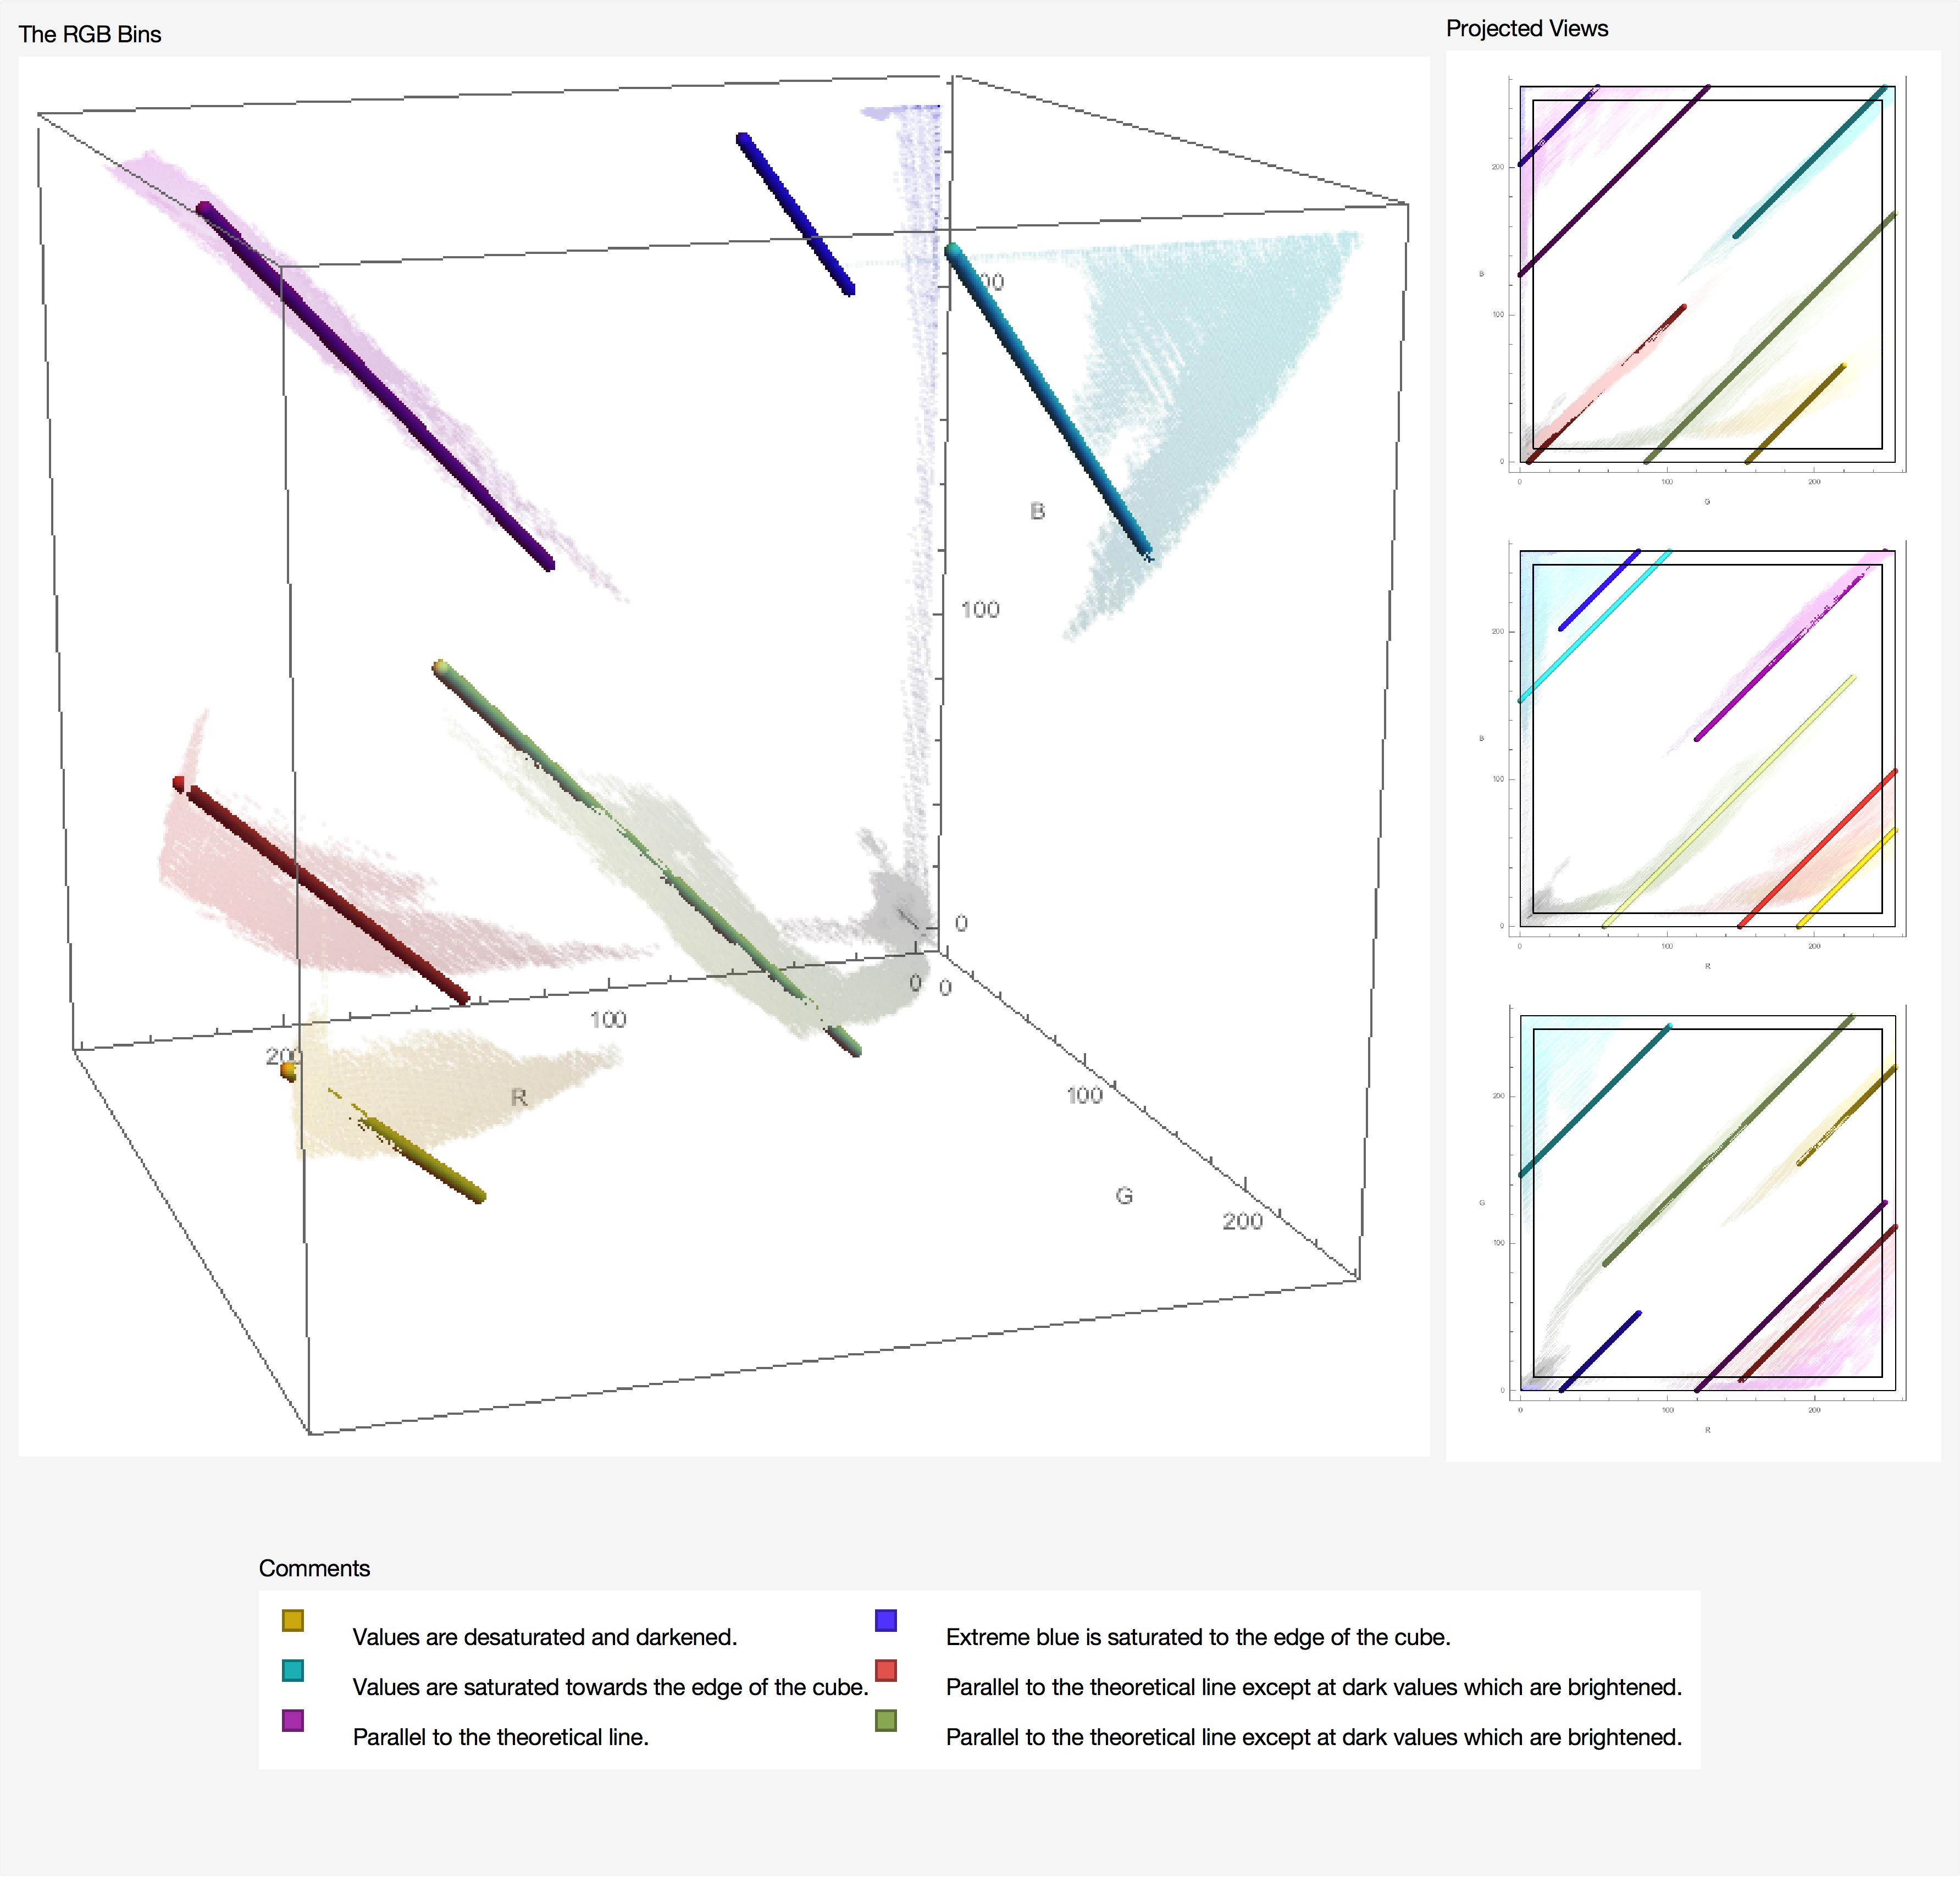
\includegraphics[width=0.98\textwidth]{Chapter3/Figs/Theory_And_Practice.jpg}
    \caption{The Bins for 6 randomly colored blobs varying only in luminosity with lines indicating the source image colors.}  \label{fig:WhitePoint}
\end{figure}

The white point for the iPhone camera was found by taking a random set of 6 colors $X=\left\{ \left\{X^1_R +\lambda, X^1_G  +\lambda, X^1_B +\lambda \right\}, \cdots \right\} $. and varying the luminosity between  $ \lambda(X)_B < \lambda  < \lambda(X)_W$. This produces a set of 6 colors which vary only in luminosity and which do not suffer from white-out or black-out. Panels of these 6 colors with randomly selected luminosity for each were presented to the camera. This produced a set of images and the statistics were collected for this set. Theoretically we expect there to be 6 distinct parallel lines which are also parallel to the line from black to the white point of the camera. If the white point of the camera is not $\left\{ 255,255,255\right\}$ then this test should allow the determination of the real white point. 

The iPhone's white point is always set to the corner of the RGB cube before the image reaches the AP layer. So, when developing an algorithm for the iPhone, white point correction is not necessary, while on other devices the algorithm may need to be adapted accordingly.
\subsection{Color Correction Pre-processing}
A second undocumented pre-processing stage became apparent while gathering skin statistics. The original approach taken used a set of photos of an individual's skin  under different lighting conditions against a constant monochromatic background captured with the iPhone camera. The background was included in order to obtain data on the edges of the skin. A background set of photos captured under the same conditions but without the presence of a hand would then be used to produce a statistical model which would be used to negate bin counts from the individual's skin set which corresponded to background values.

Surprisingly, this approached failed to work; the background was not represented well by the collected background statistics (Figure~\ref{fig:BGFailure}).

\begin{figure}[h!]
  \centering
    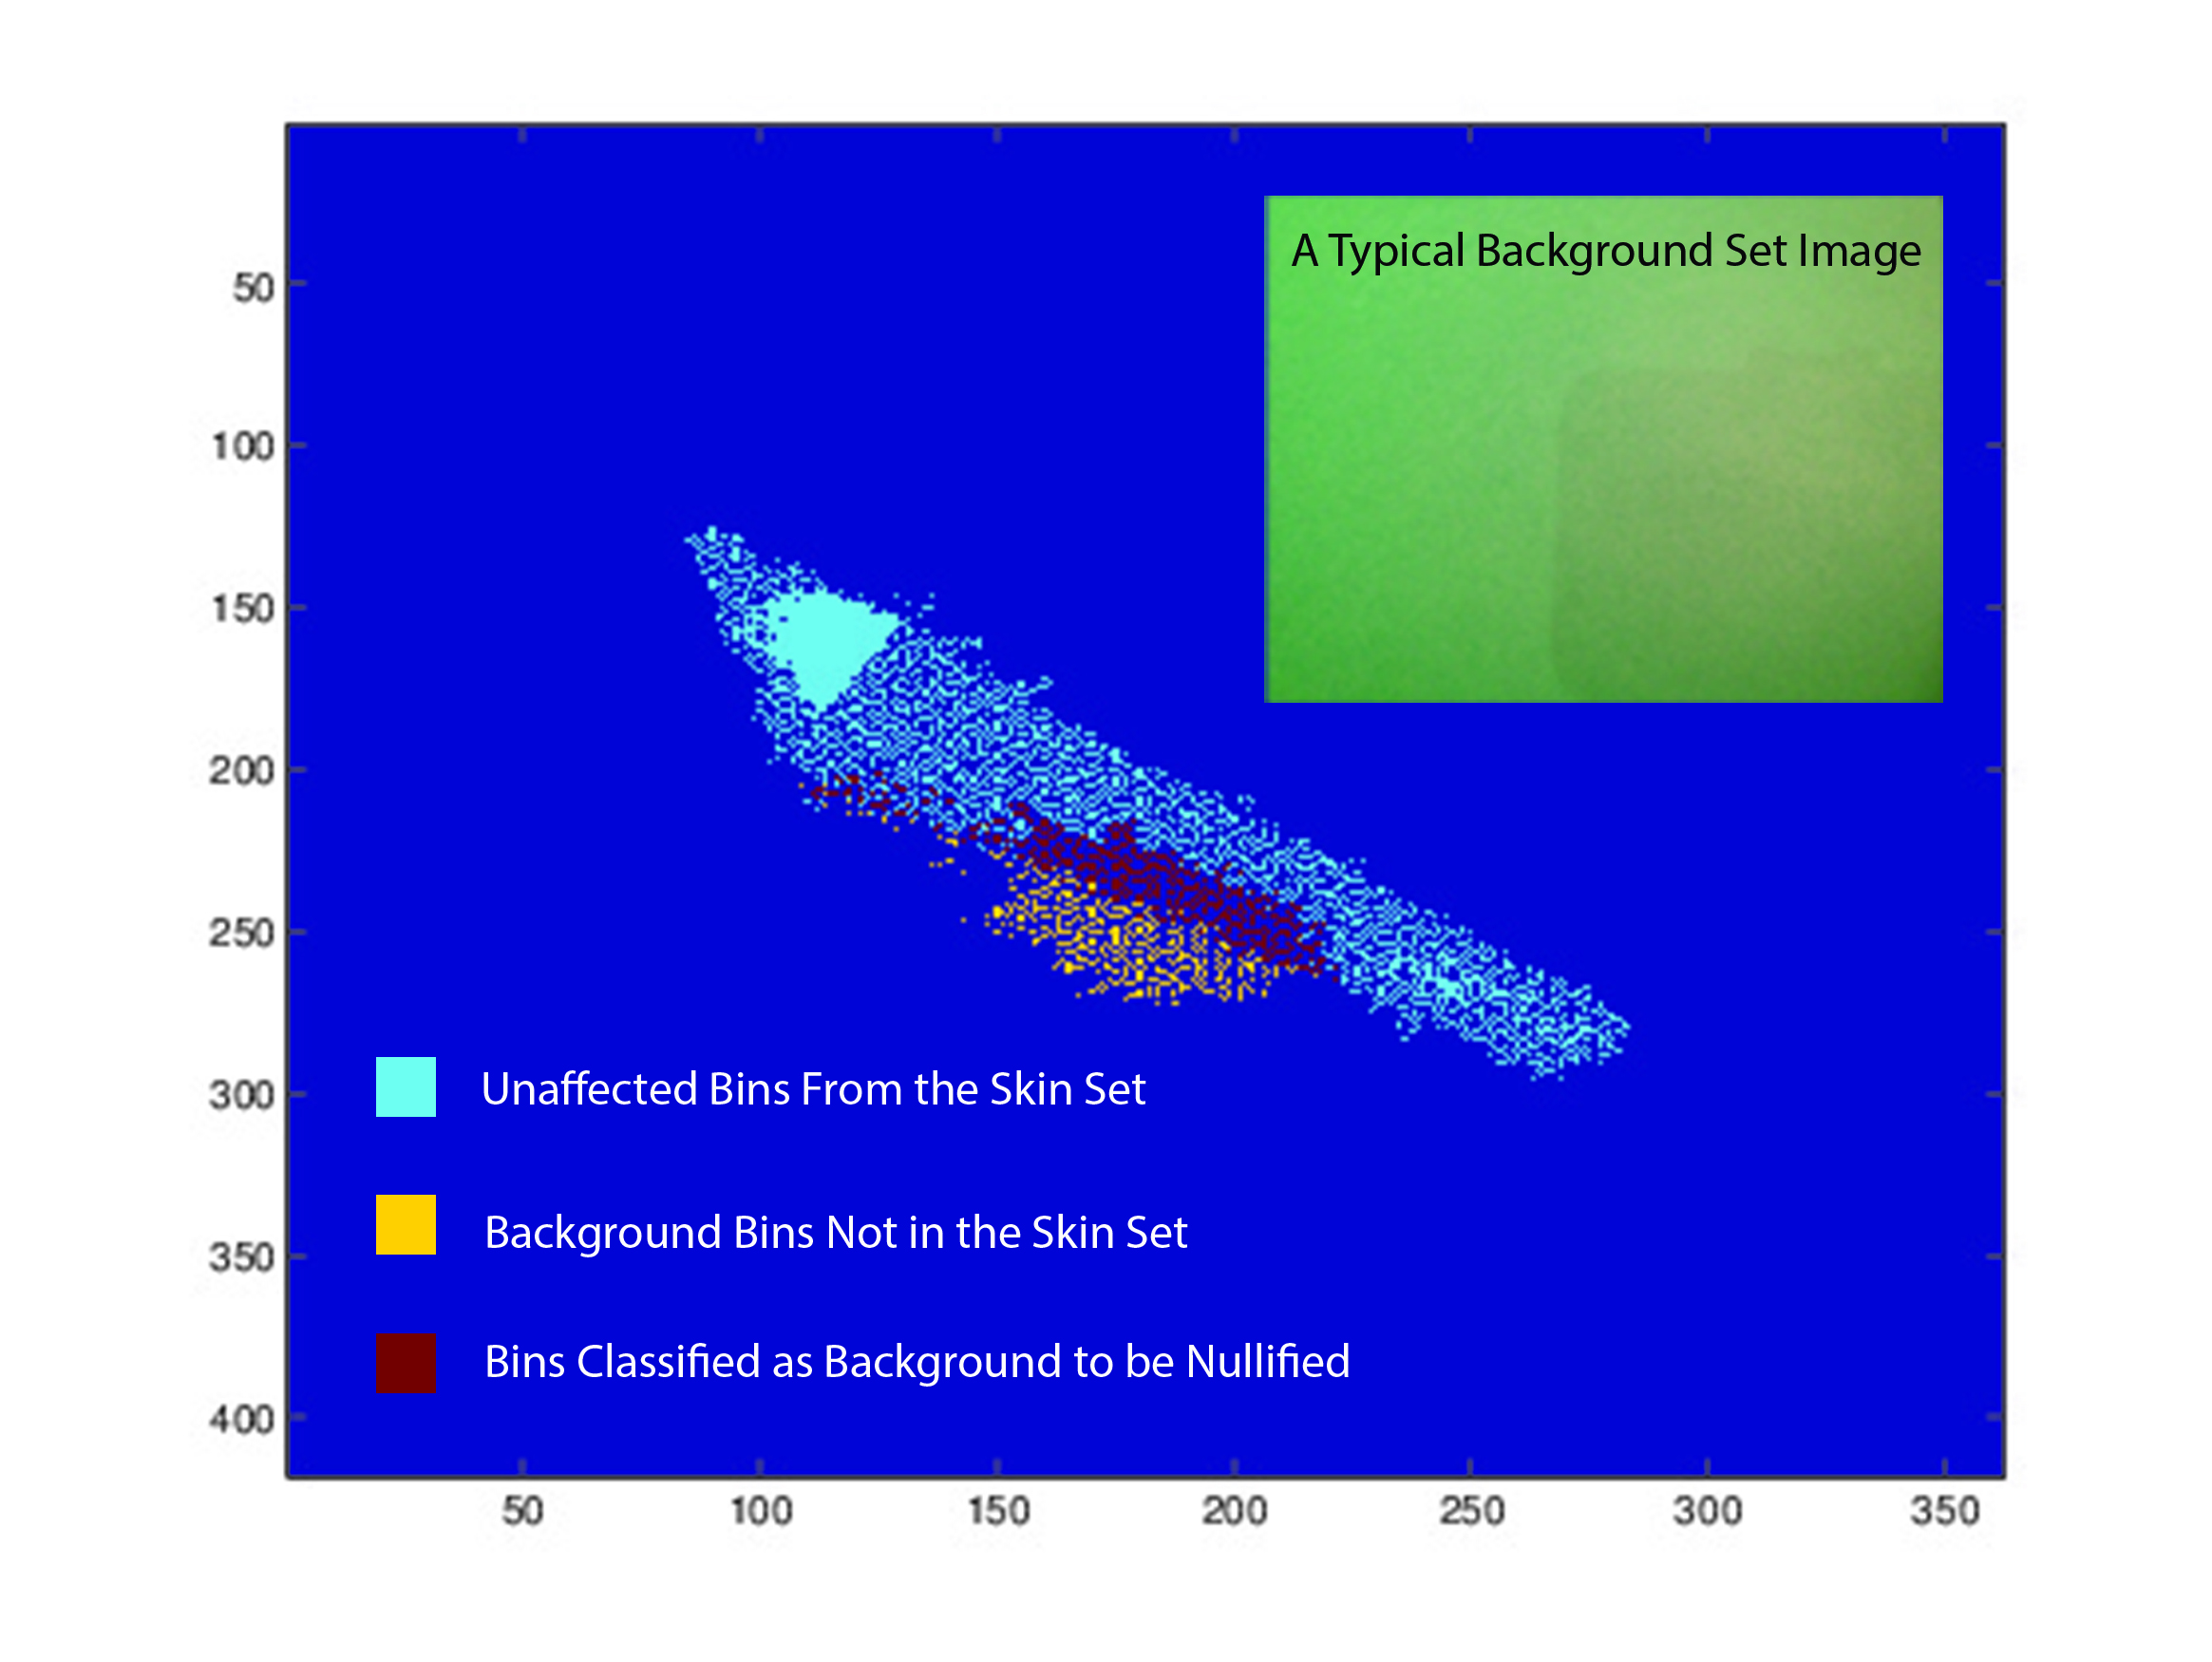
\includegraphics[width=0.95\textwidth]{Chapter3/Figs/CaCb_bg_failed.jpg}
    \caption{Initial attempt at removing background; unsuccessful.} \label{fig:BGFailure}
\end{figure}

The background statistics changed with the skin present in the photo. This is because the iPhone adjusts to images with very strong color characteristics. This color correction is an undocumented feature of the iPhone processing. The only way to compensate for this unwelcome pre-processing is to photograph the background with a strongly contrasting object present, but one which is easily cropped out of the image before the background statistics are collected. After collecting the statistics again, the result was much improved (Figure~\ref{fig:BGSuccess1}).

\begin{figure}[h!]
  \centering
    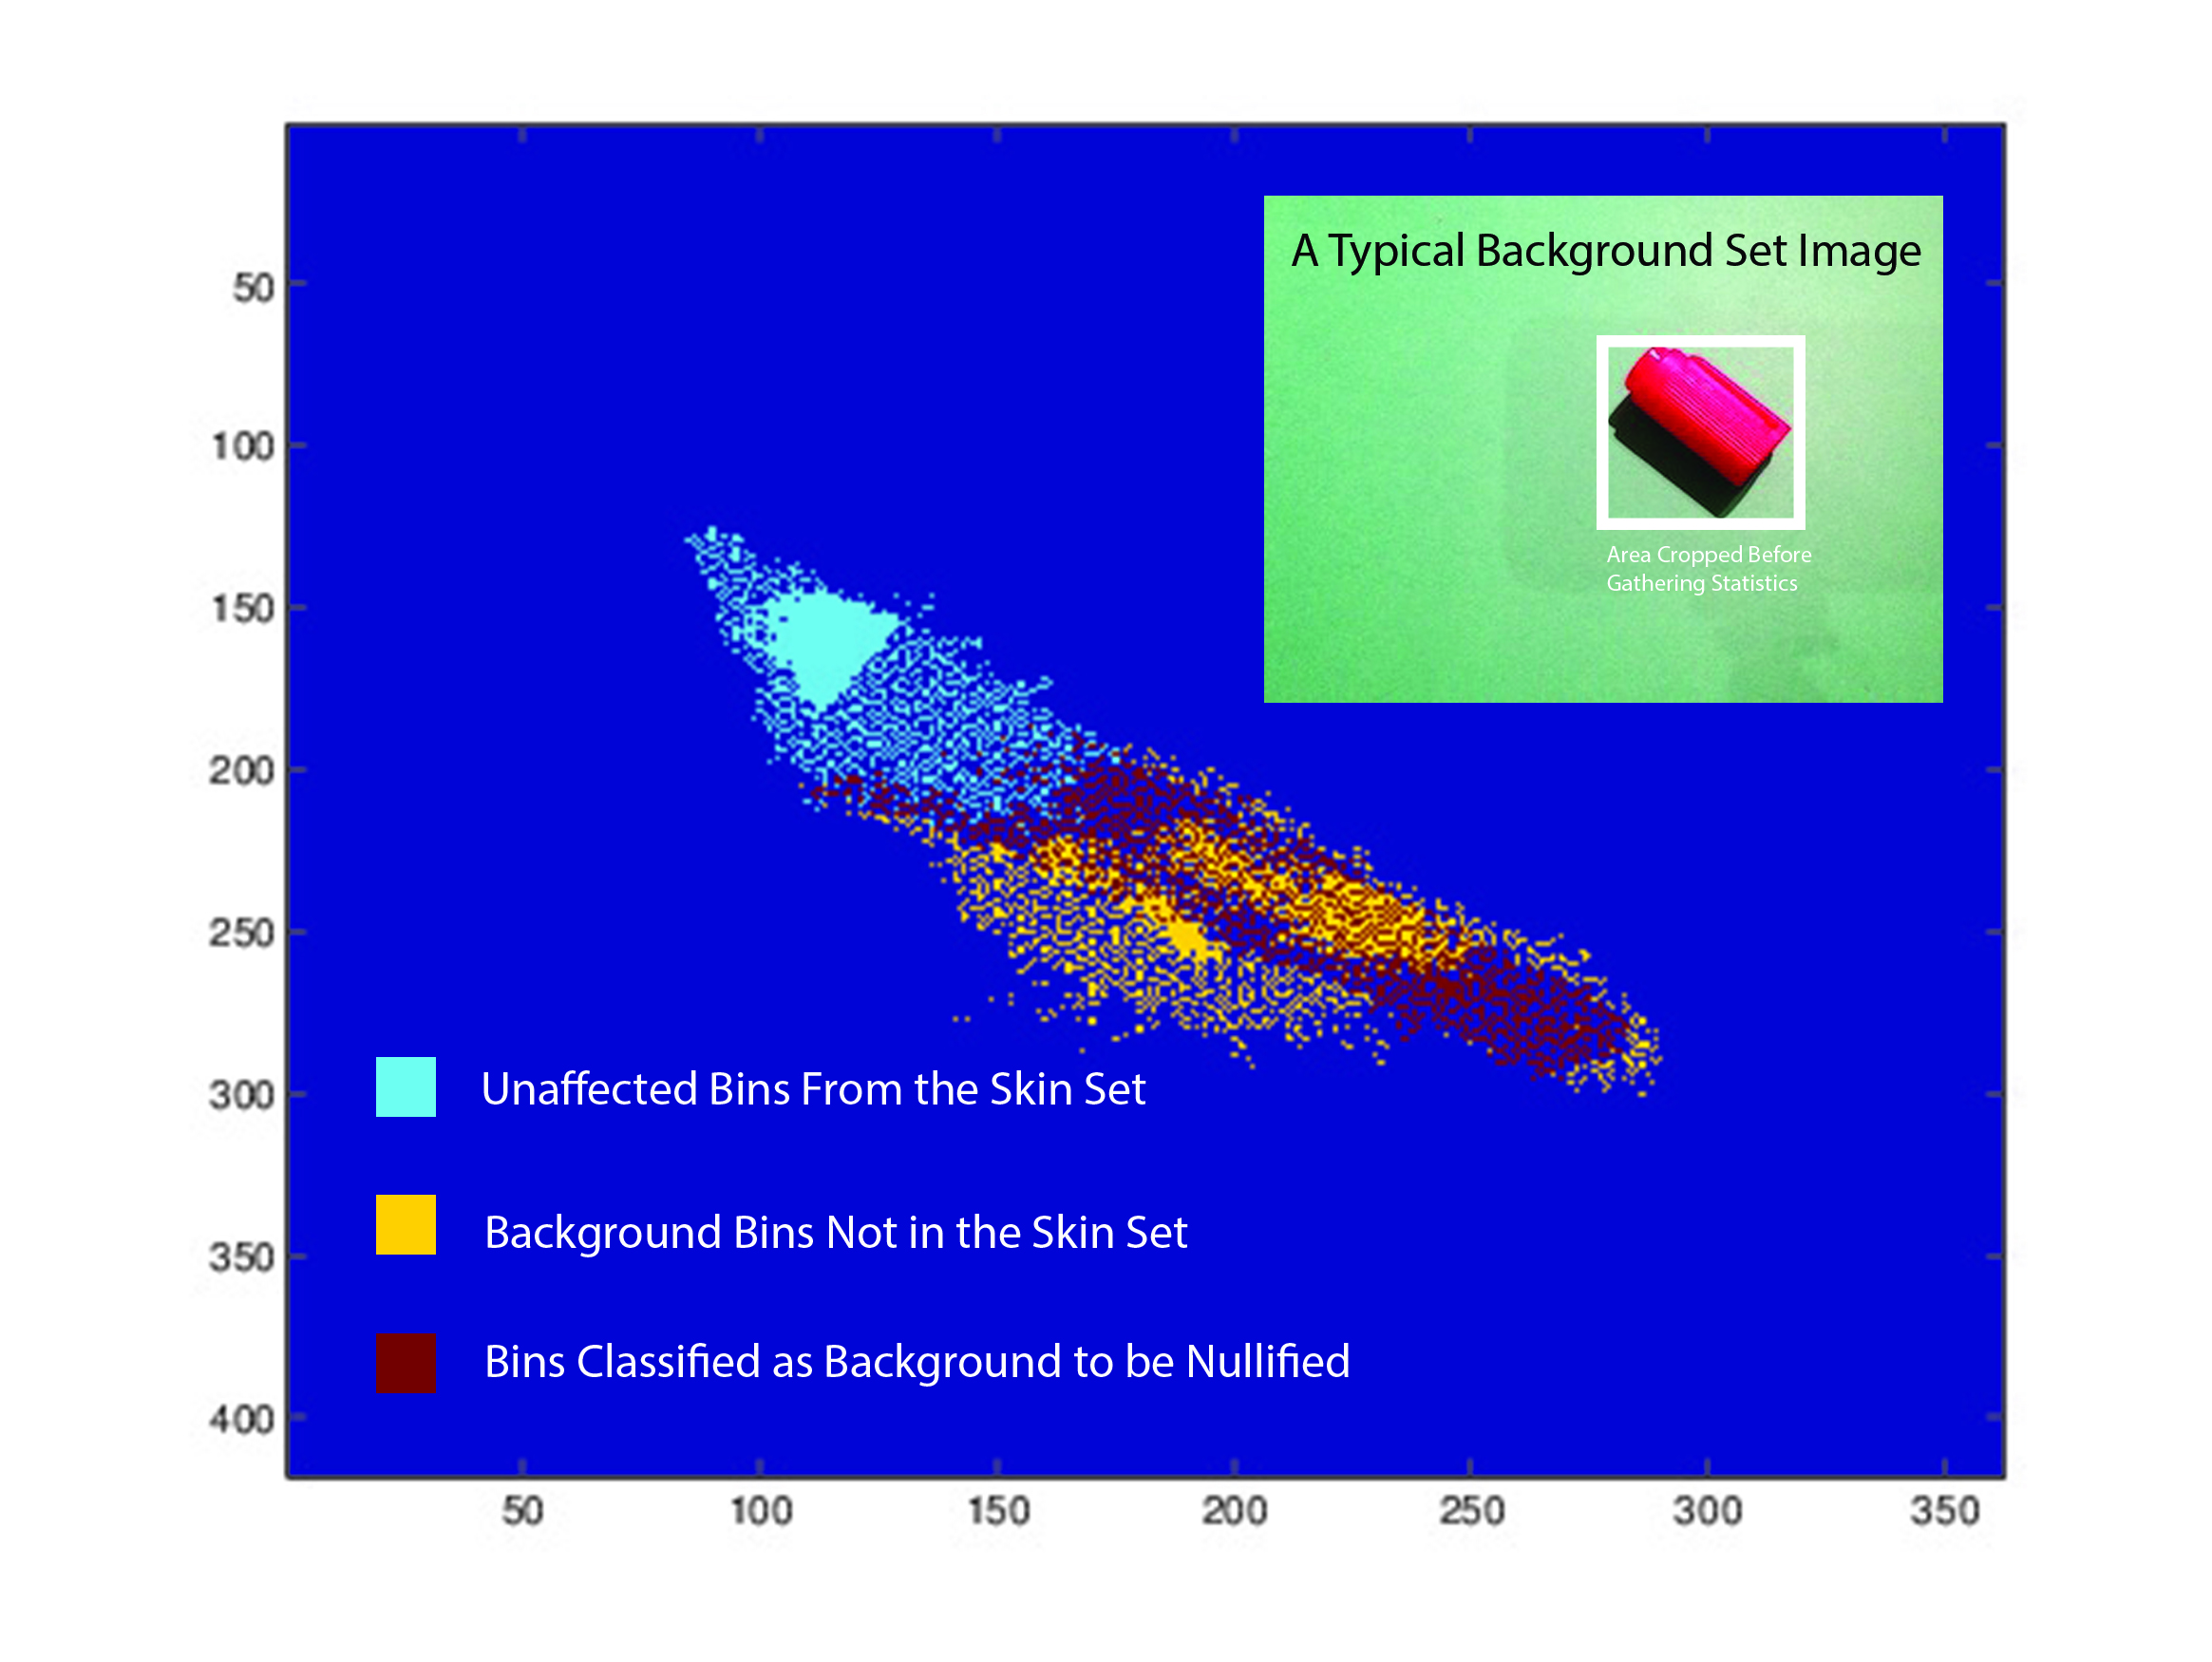
\includegraphics[width=0.80\textwidth]{Chapter3/Figs/CaCb_bg_success.jpg}
    \caption{Successful background removal.}  \label{fig:BGSuccess1}
\end{figure}

In a real world context, it is relatively safe to presume that the scene will be chromatically complex enough that the color correction won't be detrimental to detection, and perhaps even beneficial under unusual lighting conditions. But for gathering statistics, it proved to be a massive pain.

\subsection{White-Out and Black-Out}\label{sec:WhiteoutAndBlackout}
A monochromatic object with average RGB color $\mathbf{\mu}=\left\{\mu_R, \mu_G, \mu_B \right\}$ under different lighting conditions produce an in-camera value of $\left\{\mu_R +\lambda, \mu_G  +\lambda, \mu_B +\lambda \right\}$. Each channel has a numerical limit which means that when that limit is reached further change in luminosity $\lambda$ will result in a change in chromatic value. At high luminosities the colors converge on white becoming washed out. This is referred to as white-out. Similarly at low luminosities the colors converge on black which is referred to as black-out.

\begin{figure}[h!] %hi-res
  \centering
    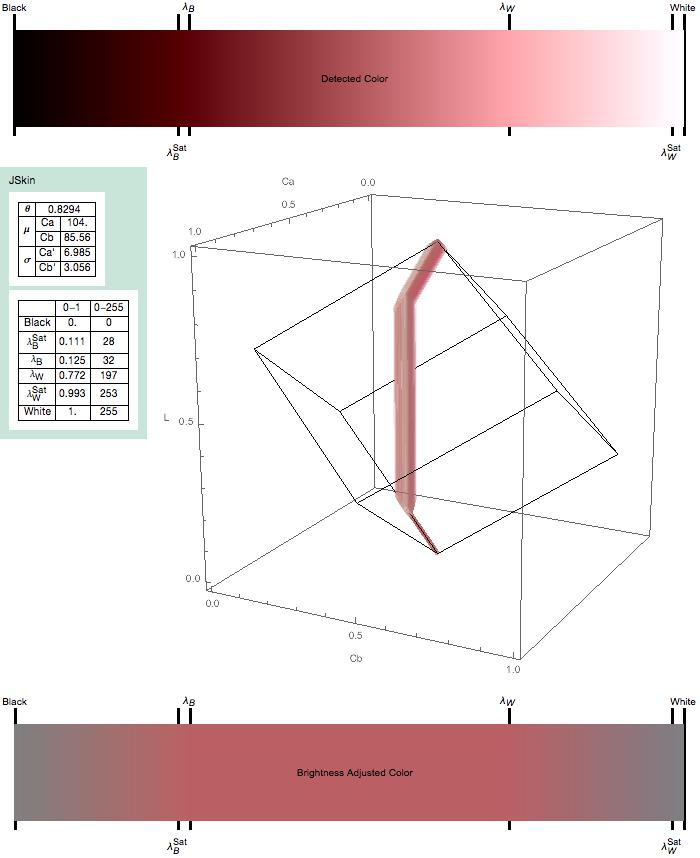
\includegraphics[width=0.80\textwidth]{Chapter3/Figs/WOBOFig.jpg}
    \caption{White-out and Black-out.}  \label{fig:WoBo1}
\end{figure}

It is reasonable to assume that pixel values which contain fully saturated channel elements are unreliable as they may be the result of white-out or black-out. Unfortunately the iPhone also performs an auto brightness and contrast adjustment moving pixel values away from the sides of the RGB cube. The result of this processing is that the values with a luminosity above $\lambda_w$ and below $\lambda_b$ are unreliable.

\section{Algorithm for Generating the Model}\label{sec:AlgorithmForGeneratingModel}
Here we present the algorithm which is used to generate the chromatic model. It's assumed we have RGB image sets for the target with simple, monochromatic backgrounds.

%\animategraphics[loop,autoplay,controls]{12}{Chapter3/Figs/FSkin/RGB_FSkin_Bin_Animation/frame}{0001}{0025}
%\animategraphics[loop,autoplay,controls]{12}{Chapter3/Figs/FSkin/RGB_FSkin_Bin_Skinned_Animation/frame}{0001}{0025}
%\animategraphics[loop,autoplay,controls]{12}{Chapter3/Figs/FSkin/RGB_FSkin_Bin_Skinned_Rot_Animation/frame}{0001}{0025}
%\animategraphics[loop,autoplay,controls]{12}{Chapter3/Figs/FSkin/RGB_FSkin_Bin_Skinned_Rot_TopTail_Animation/frame}{0001}{0025}


%\includemedia[
%  label=cube_test,
%  width=0.7\linewidth,height=0.7\linewidth,
%  addresource=Chapter3/Figs/Animation/RGB_FSkin_Hand_Bin.swf, %two video files
%  transparent,
%  activate=pageopen,
%  flashvars={
%    source=Chapter3/Figs/Animation/RGB_FSkin_Hand_Bin.swf
%   &loop=true
%   &scaleMode=letterbox
%  }
%]{}{Chapter3/Figs/Animation/RGB_FSkin_Hand_Bin.swf}


\subsection{RGB Bin Allocation}\label{sec:RGBBinAllocation}


% Choose an individual for the plots
%\def\individual{FJN}
\def\individual{FSkin}
%\def\individual{JSkin}
%\def\individual{NSkin}


\begin{figure}[h!]
  \centering
    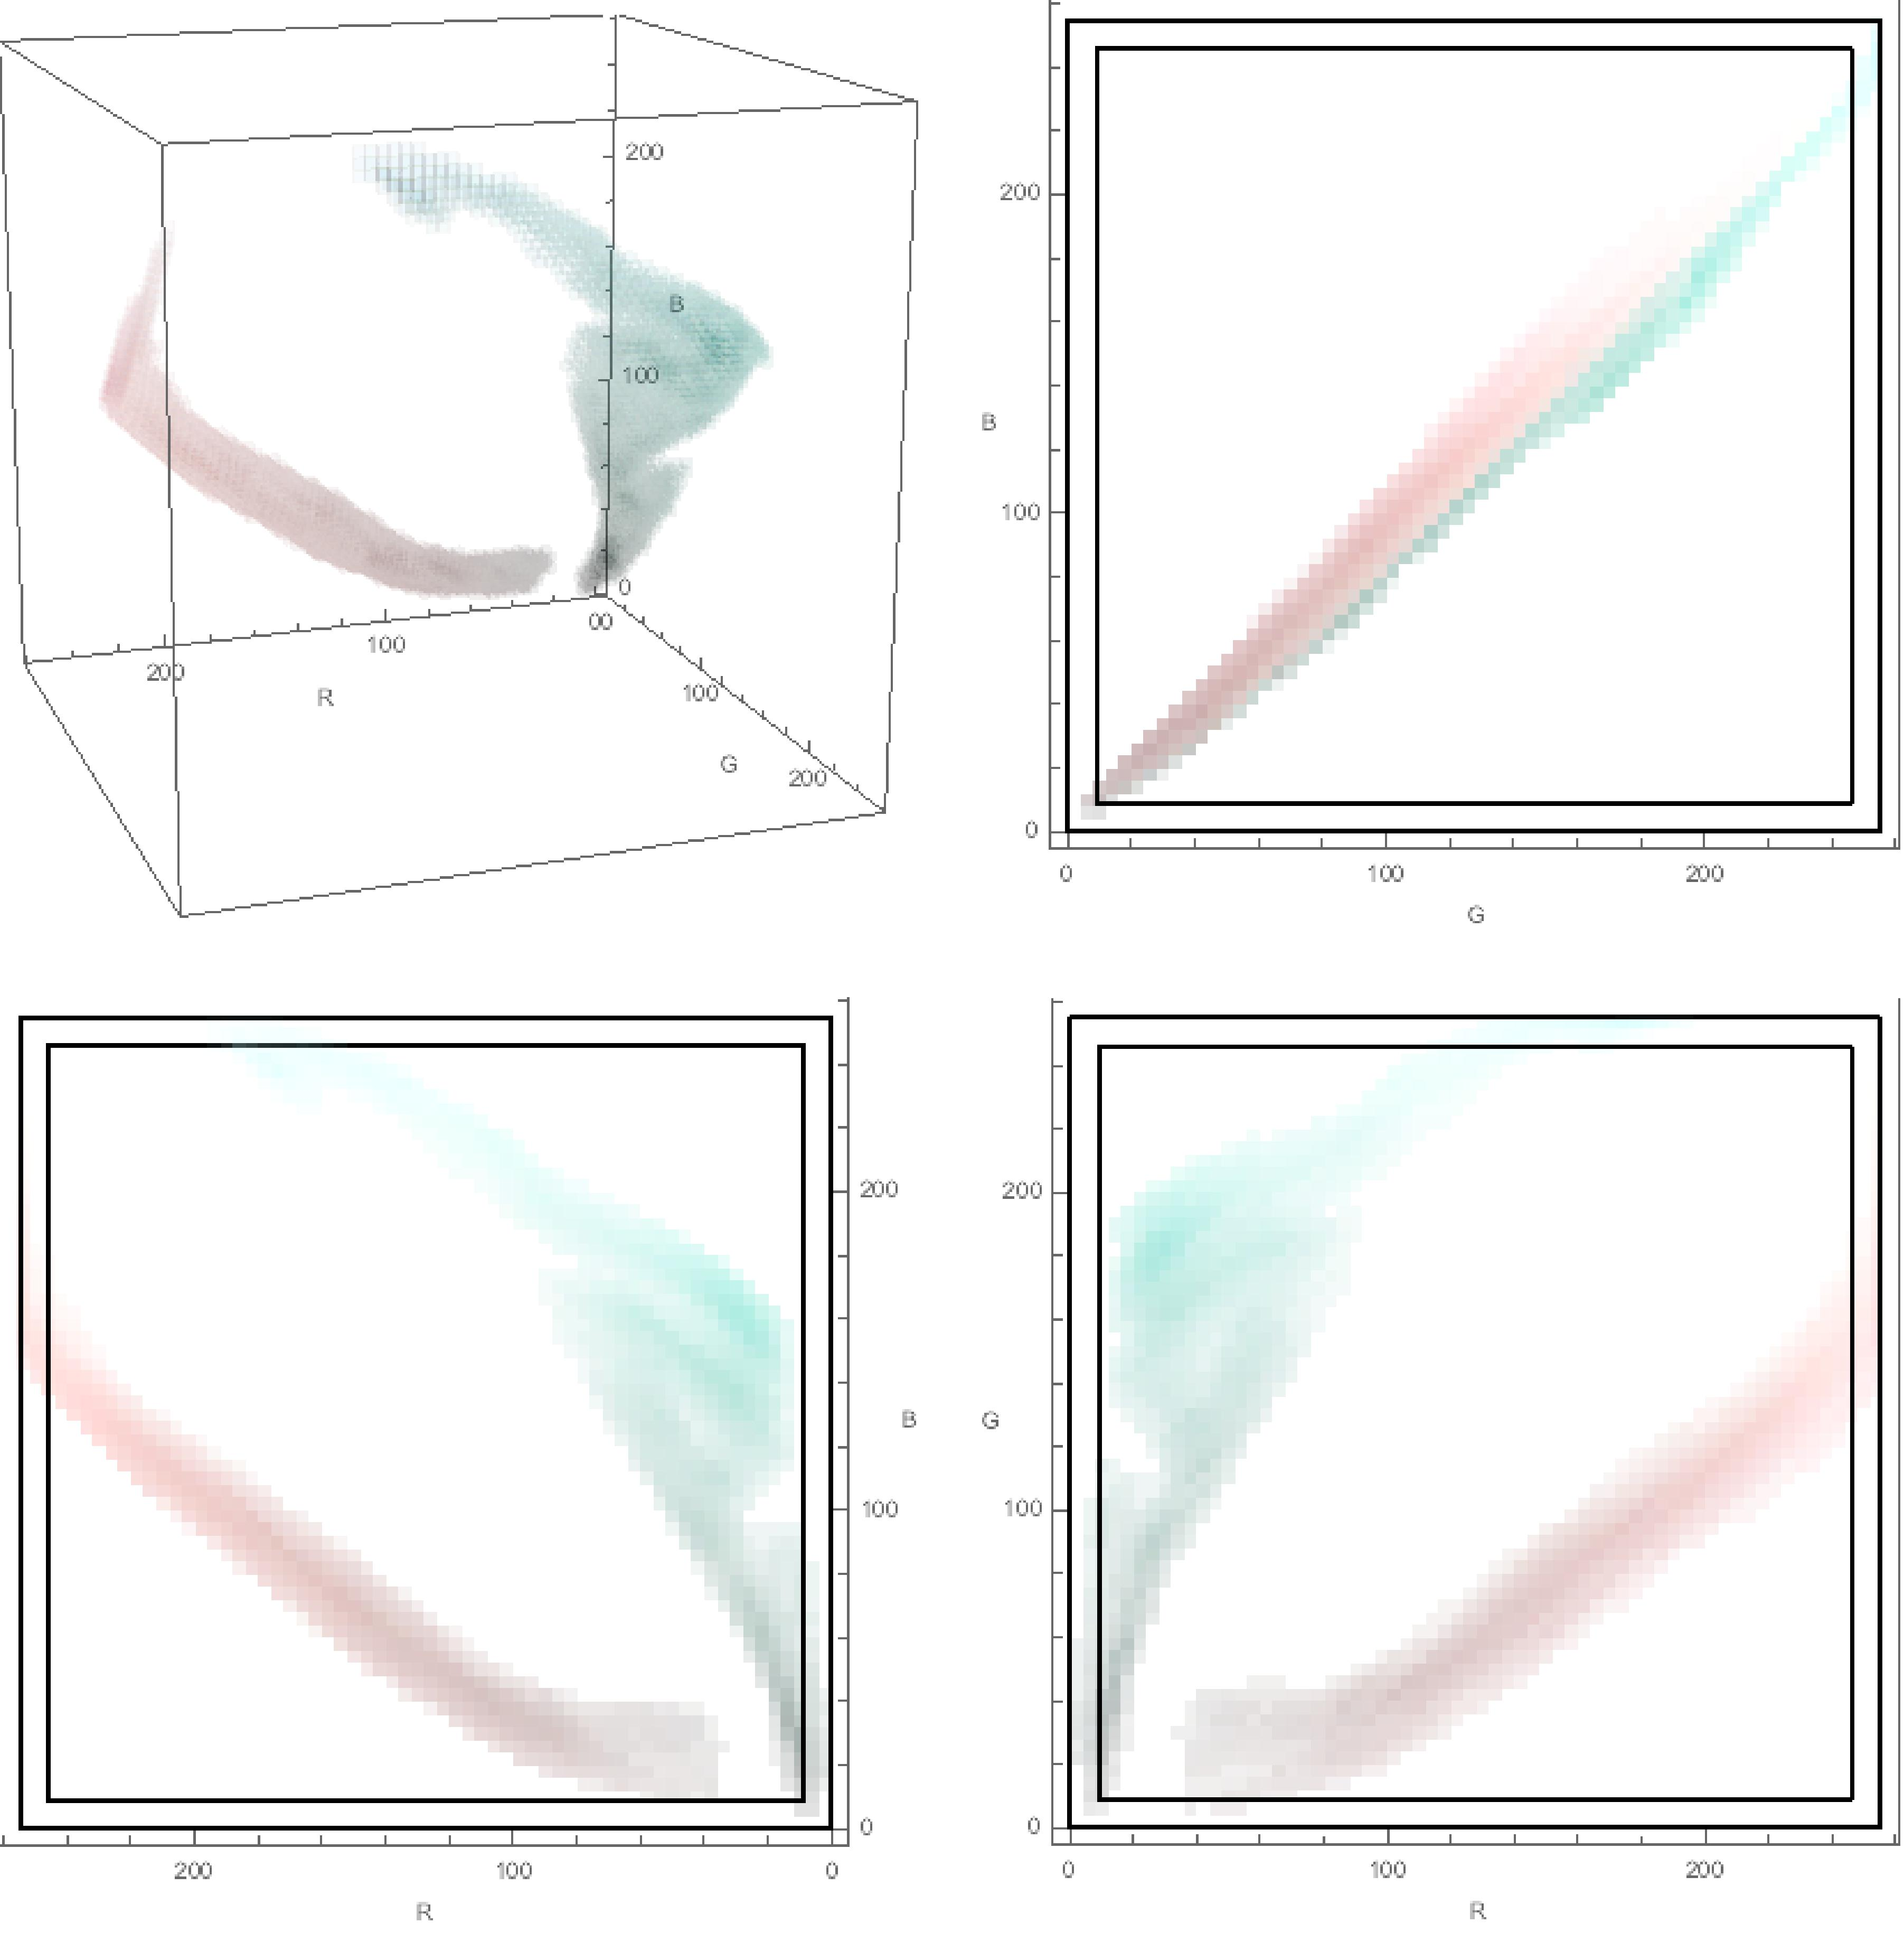
\includegraphics[width=0.9\textwidth]{Chapter3/Figs/\individual/Fill_the_Bins.jpg}
        \caption{\textbf{The 3D RGB histogram}. Distinct distributions can be seen for the Skin and the background. Here the bin color corresponds to the color which that bin represents and the opacity indicates the frequency of that bin value. }  \label{fig:Fill_the_Bins}
    \end{figure}

The first problem is that we have a large image set with large images. We're only interested in the individual pixel values so we produce a 3D histogram with one bin for each RGB combination giving 256x256x256 bins. This is a large data set but it's easier to work with than the set of images and is guaranteed to contain all the relevant information for the statistics.

The histogram bin counting algorithm is written in MATLAB. It runs through each pixel in the image set, proceeding as follows:

\begin{itemize}
\item Increment the corresponding bin.
\item Increment the total pixel count.
\item Is the current bin count larger than the largest bin count so far? If so, increment the largest bin count.
\end{itemize}

So now we have a 3D histogram with a total bin count and a largest bin count.


\subsection{Skinning the Bins}\label{sec:SkinningTheBins}

\begin{figure}[h!] %hi-res
  \centering
    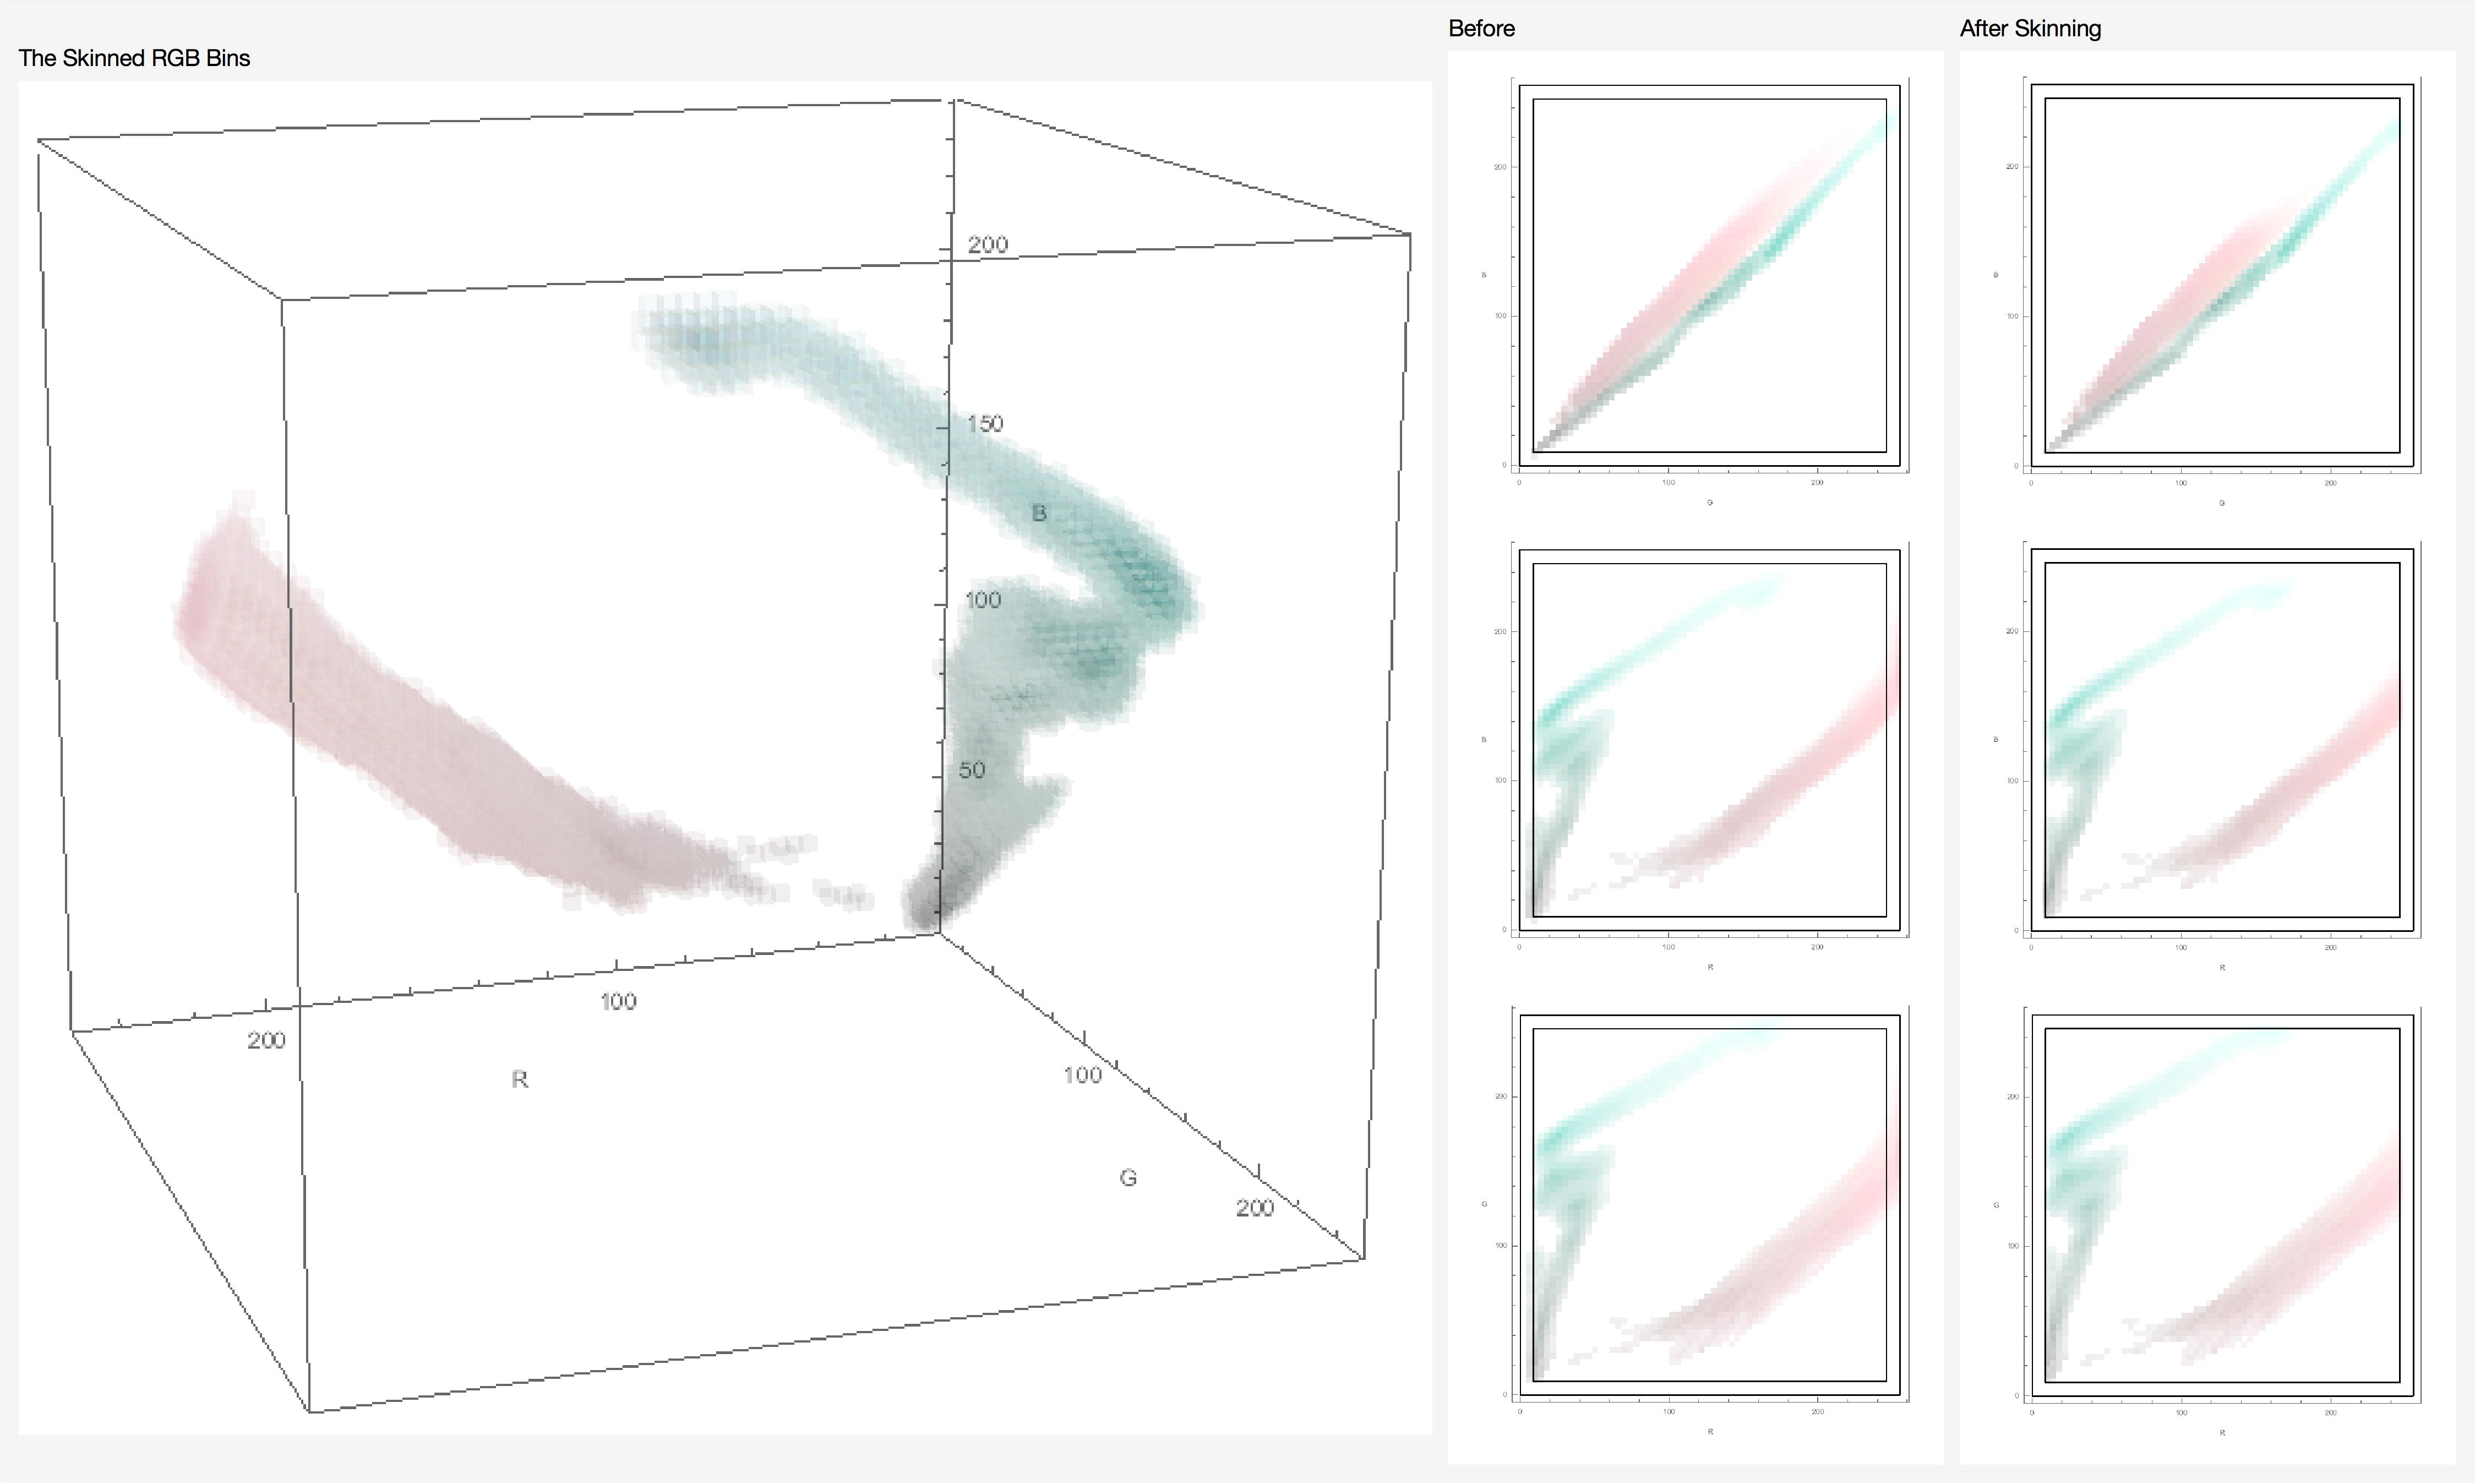
\includegraphics[width=1.0\textwidth]{Chapter3/Figs/\individual/Skin_the_Bins.jpg}
        \caption{\textbf{The 3D RGB histogram after 'skinning'}. Distinct distributions can be seen for the Skin and the background. Here the bin color corresponds to the color which that bin represents and the opacity indicates the frequency of that bin value. Bin counts outside the black lines are set to zero. }  \label{fig:Skin_the_Bins}
    \end{figure}

Next, the bins which are at the extreme edges (i.e. the ones which correspond to the outer faces of the RGB cube) are set equal to 0 with a specified depth. For example: if a depth of 3 is requested, bins of positions 0, 1 and 2, and 253, 254 and 255 are set to 0 in all three dimensions, and the total pixel count is adjusted to compensate for the nulled bin counts. This is done to address problems of white-out and black-out as described in \ref{sec:WhiteoutAndBlackout}.



It should be noted that the reason the RGB cube is skinned before rotation is because it's not as easy to do in the rotated color-space.


\subsection{Rotating the Bins}\label{sec:RotatingTheBins}

\begin{figure}[h!] %hi-res
  \centering
    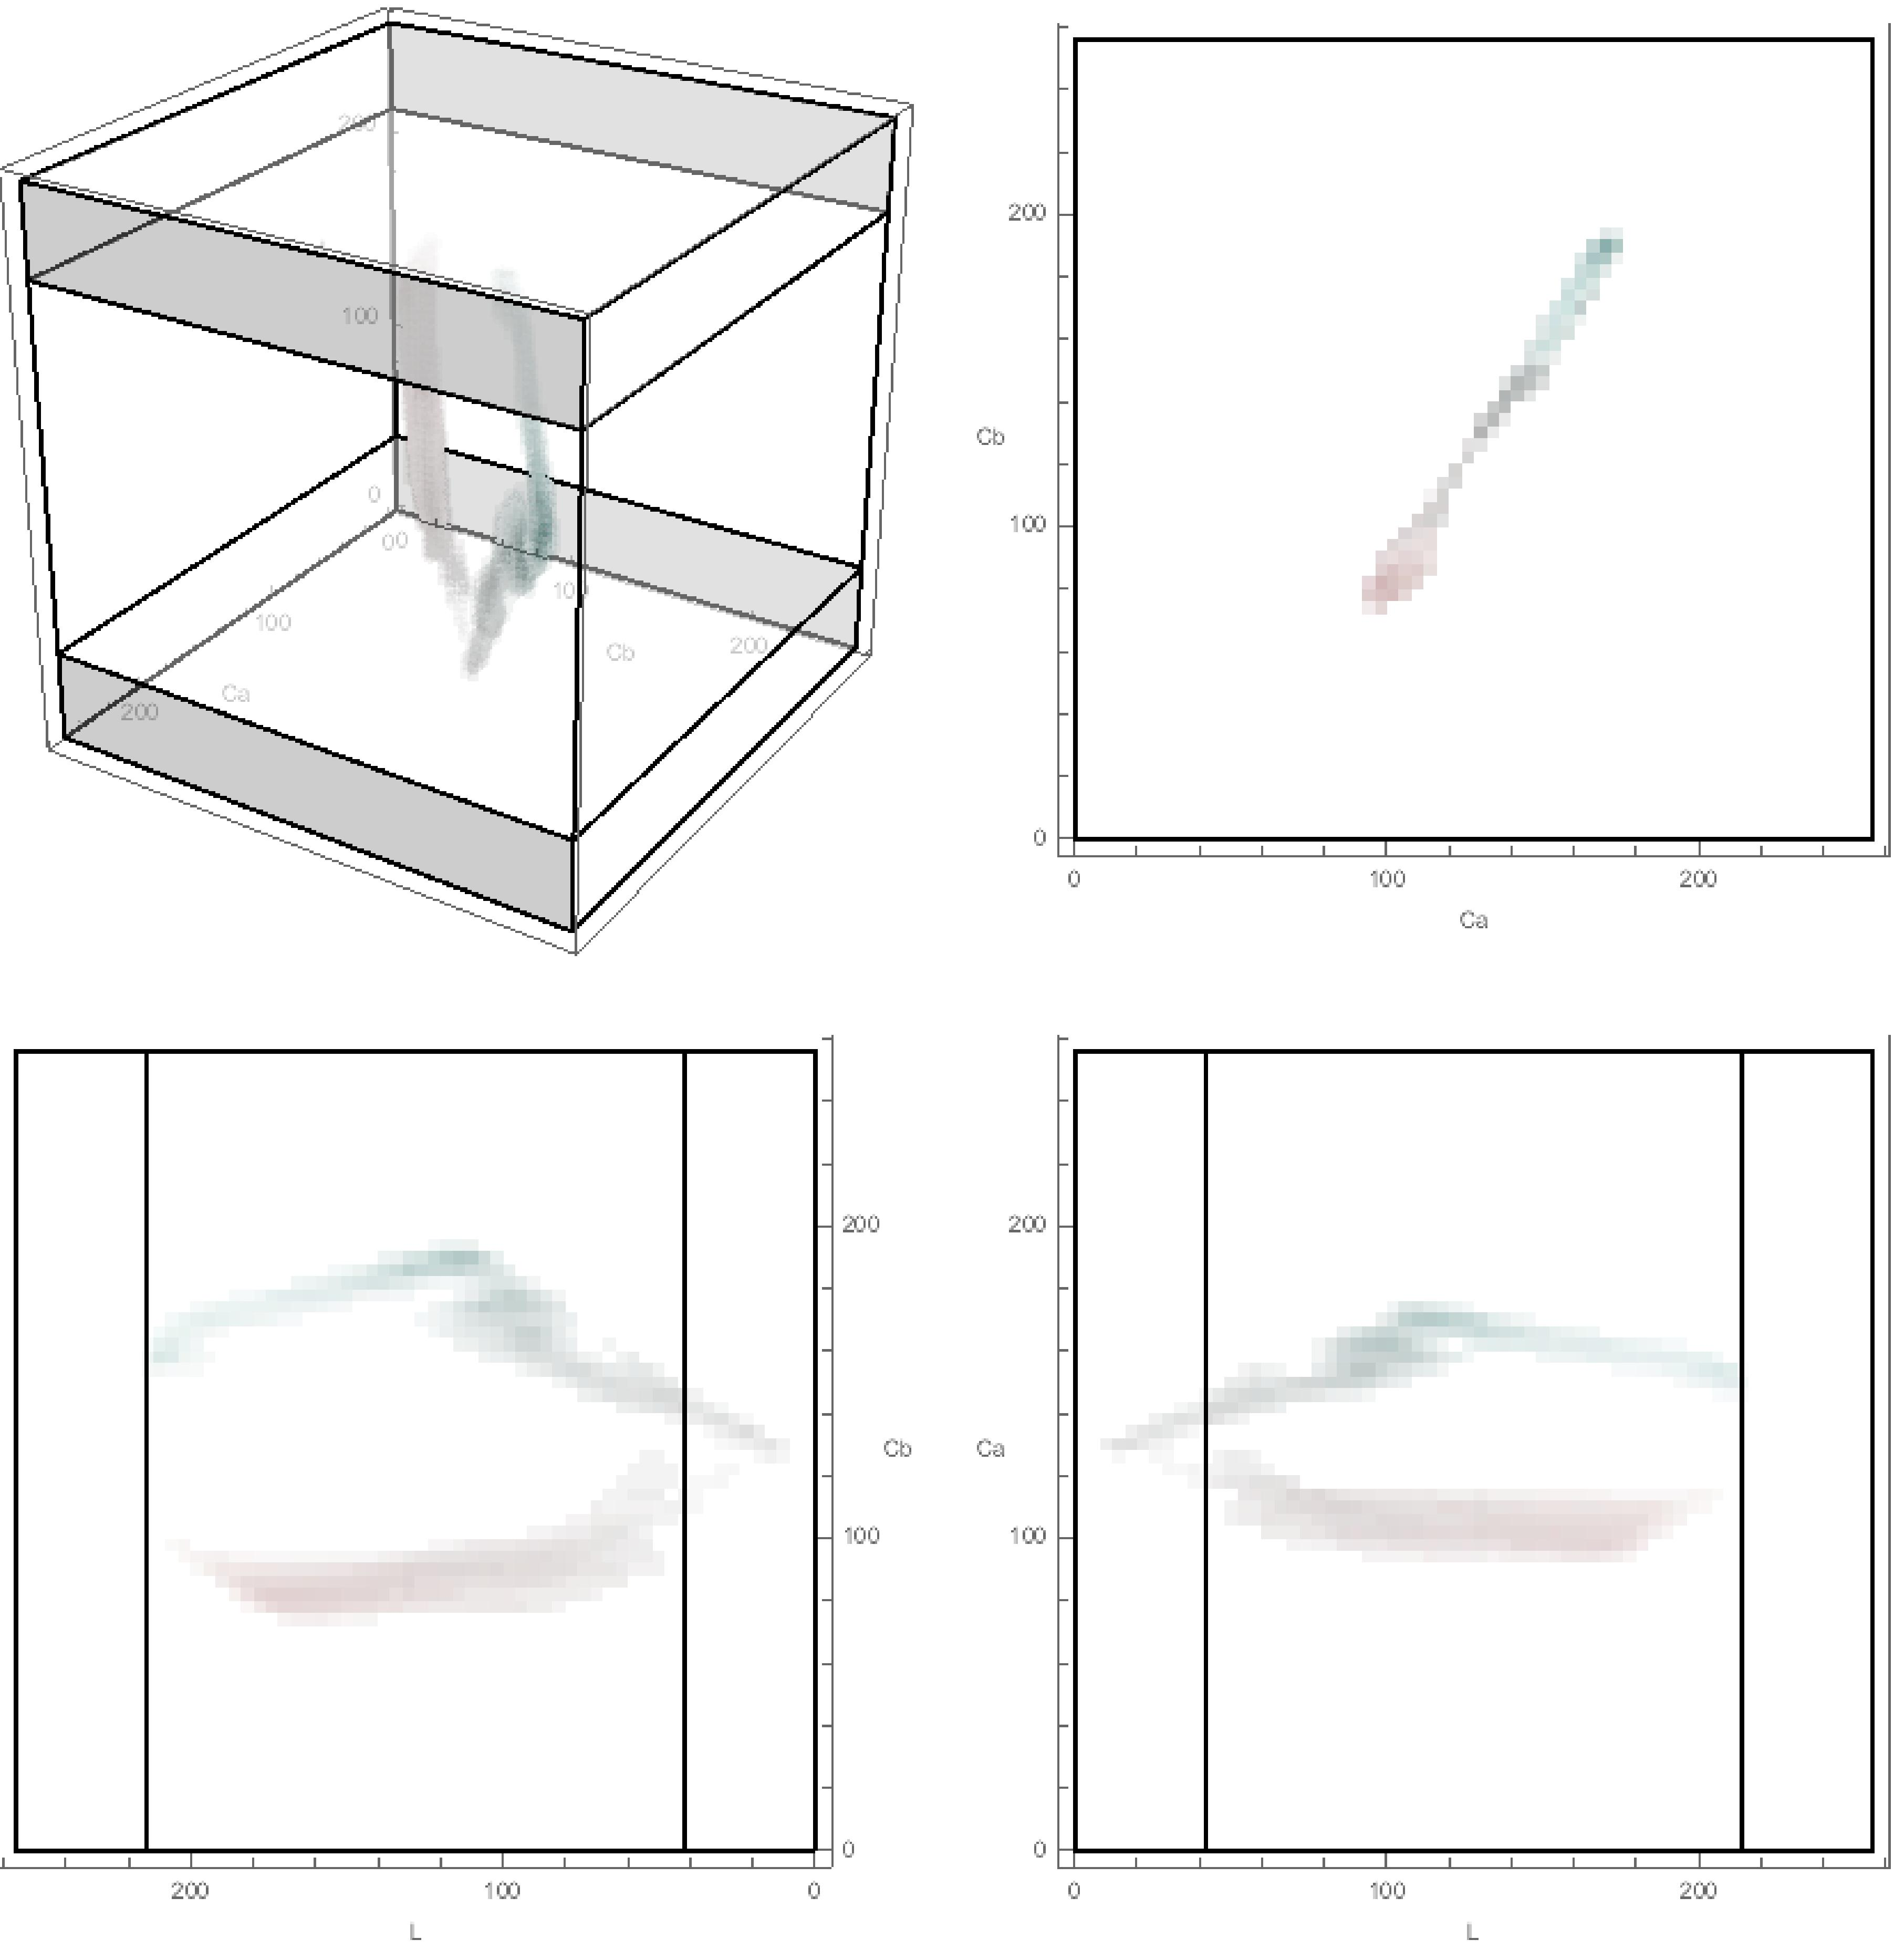
\includegraphics[width=1.0\textwidth]{Chapter3/Figs/\individual/Rotate_the_Bins.jpg}
        \caption{\textbf{The 3D RGB histogram after rotation}. The skin and background distributions can be seen for the Skin and the background. Here the bin color corresponds to the color which that bin represents and the opacity indicates the frequency of that bin value. Bin counts outside the black lines are set to zero. }   \label{fig:Rotate_the_Bins}
\end{figure}

Because each of the bins corresponds to just one RGB value, we can find the equivalent bin in the LCaCb space simply by rotating the bin index. This is done using the normalized rotation as described in Chapter 2. The normalized rotation is used as we desire the mean $\mu$ and standard deviation $\sigma$ to be specified in the $0:1$ range, which is easier to find where all the axes are of the same length. With this done, we now have a set of bins in the LCaCb color-space equivalent to that which would be found if we had applied the transform to each of the images and then collected the statistics from the transformed images.





\subsection{Top and Tail}\label{sec:TopAndTail}

\begin{figure}[h!] %hi-res
  \centering
    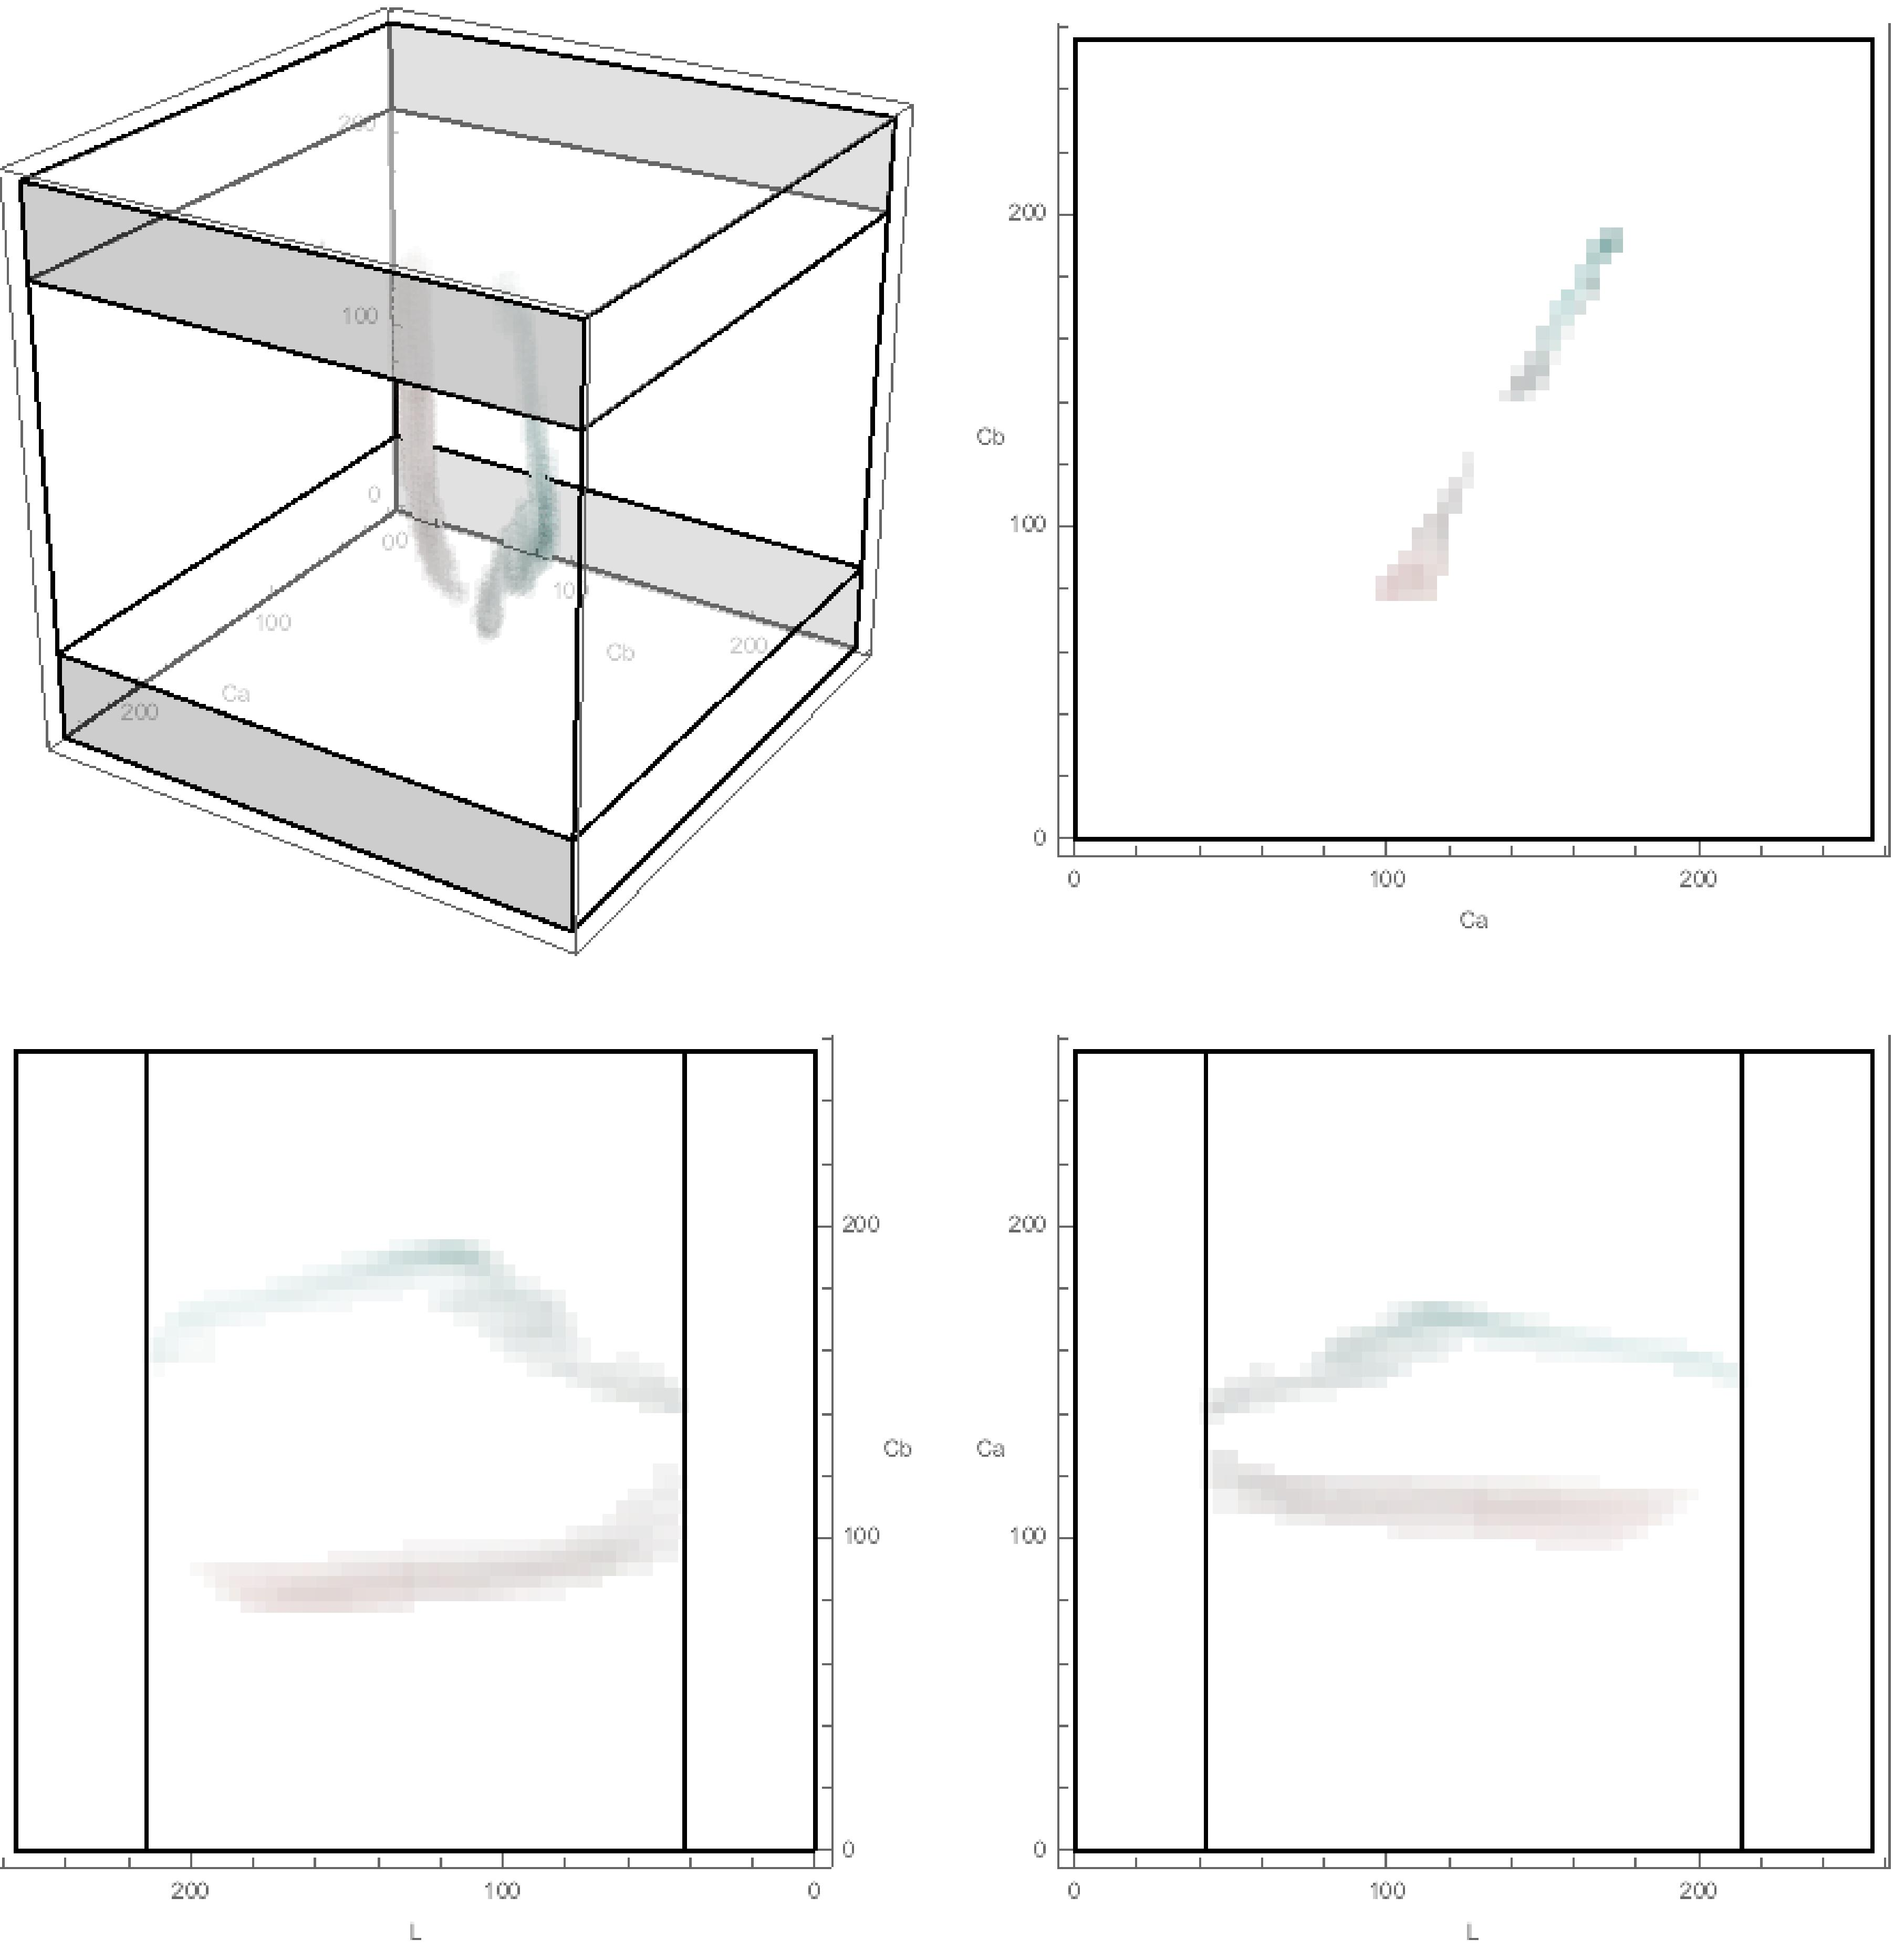
\includegraphics[width=0.9\textwidth]{Chapter3/Figs/\individual/Top_and_Tail_the_Bins.jpg}
        \caption{Filling the RGB Bins}  \label{fig:Top_and_Tail_the_Bins}
    \end{figure}


Naively collapsing the bins along the luminosity axis artificially skews the chromatic distribution along the axis which passed through the luminosity axis; this is easily explained due to white-out and black-out (\ref{sec:WhiteoutAndBlackout}). 
Although we've "skinned" the bins, the white and black tips of the cube suffer from white-out and black-out more than any other regions, and there's a tendency for pixel values to converge under the white point and the black point without necessarily hitting the side of the cube first due to the iPhone contrast and brightness adjustment. This can be seen in Figure   \ref{fig:Top_and_Tail_the_Bins}. 

We collapse the bins excluding the bins which are clearly suffering from white-out and black-out. This could be done mathematically by taking the bin of the distribution which is furthest from the luminosity axis, and then finding the intersection with the RGB cube when this chromatic value is at its limits, just before it reaches the edge of the cube where it suffers from white-out or black-out. But it's a simple matter to look at the three projections of the 3D LCaCb bins and manually determine the limits for the valid region.


\subsection{Collapsing the Bins}\label{sec:CollapsingTheBins}

\begin{figure}[h!]
  \centering
    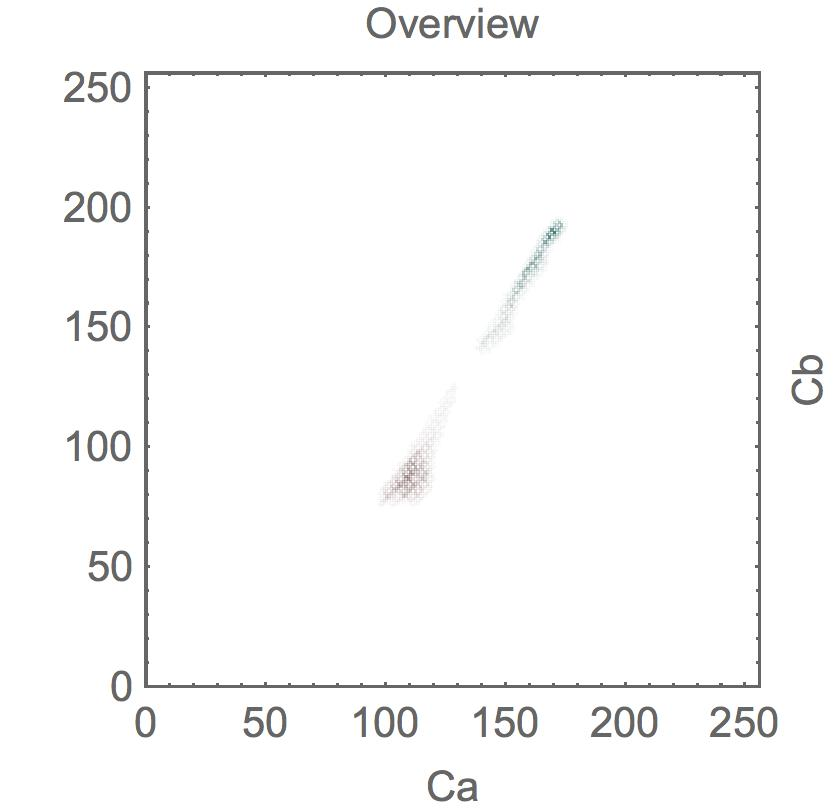
\includegraphics[width=0.6\textwidth]{Chapter3/Figs/\individual/Collapse_the_Bins.jpg}
        \caption{\textbf{The 2D histogram after summing along the luminosity axis}. The color corresponds to the chromatic value of the bin at average luminosity. The opacity corresponds to the frequency of the chromatic value. }  \label{fig:Collapse_the_Bins}
    \end{figure}
    
Because we're modelling the chromatic space and not the luminosity, we now collapse the 3D histogram by summing the bin values along the luminosity axis. So, we now have a 2D histogram in CaCb chromatic space.





\subsection{De-Speckling the Bin Values}\label{sec:DeSpeckle}

\begin{figure}[h!]
  \centering
    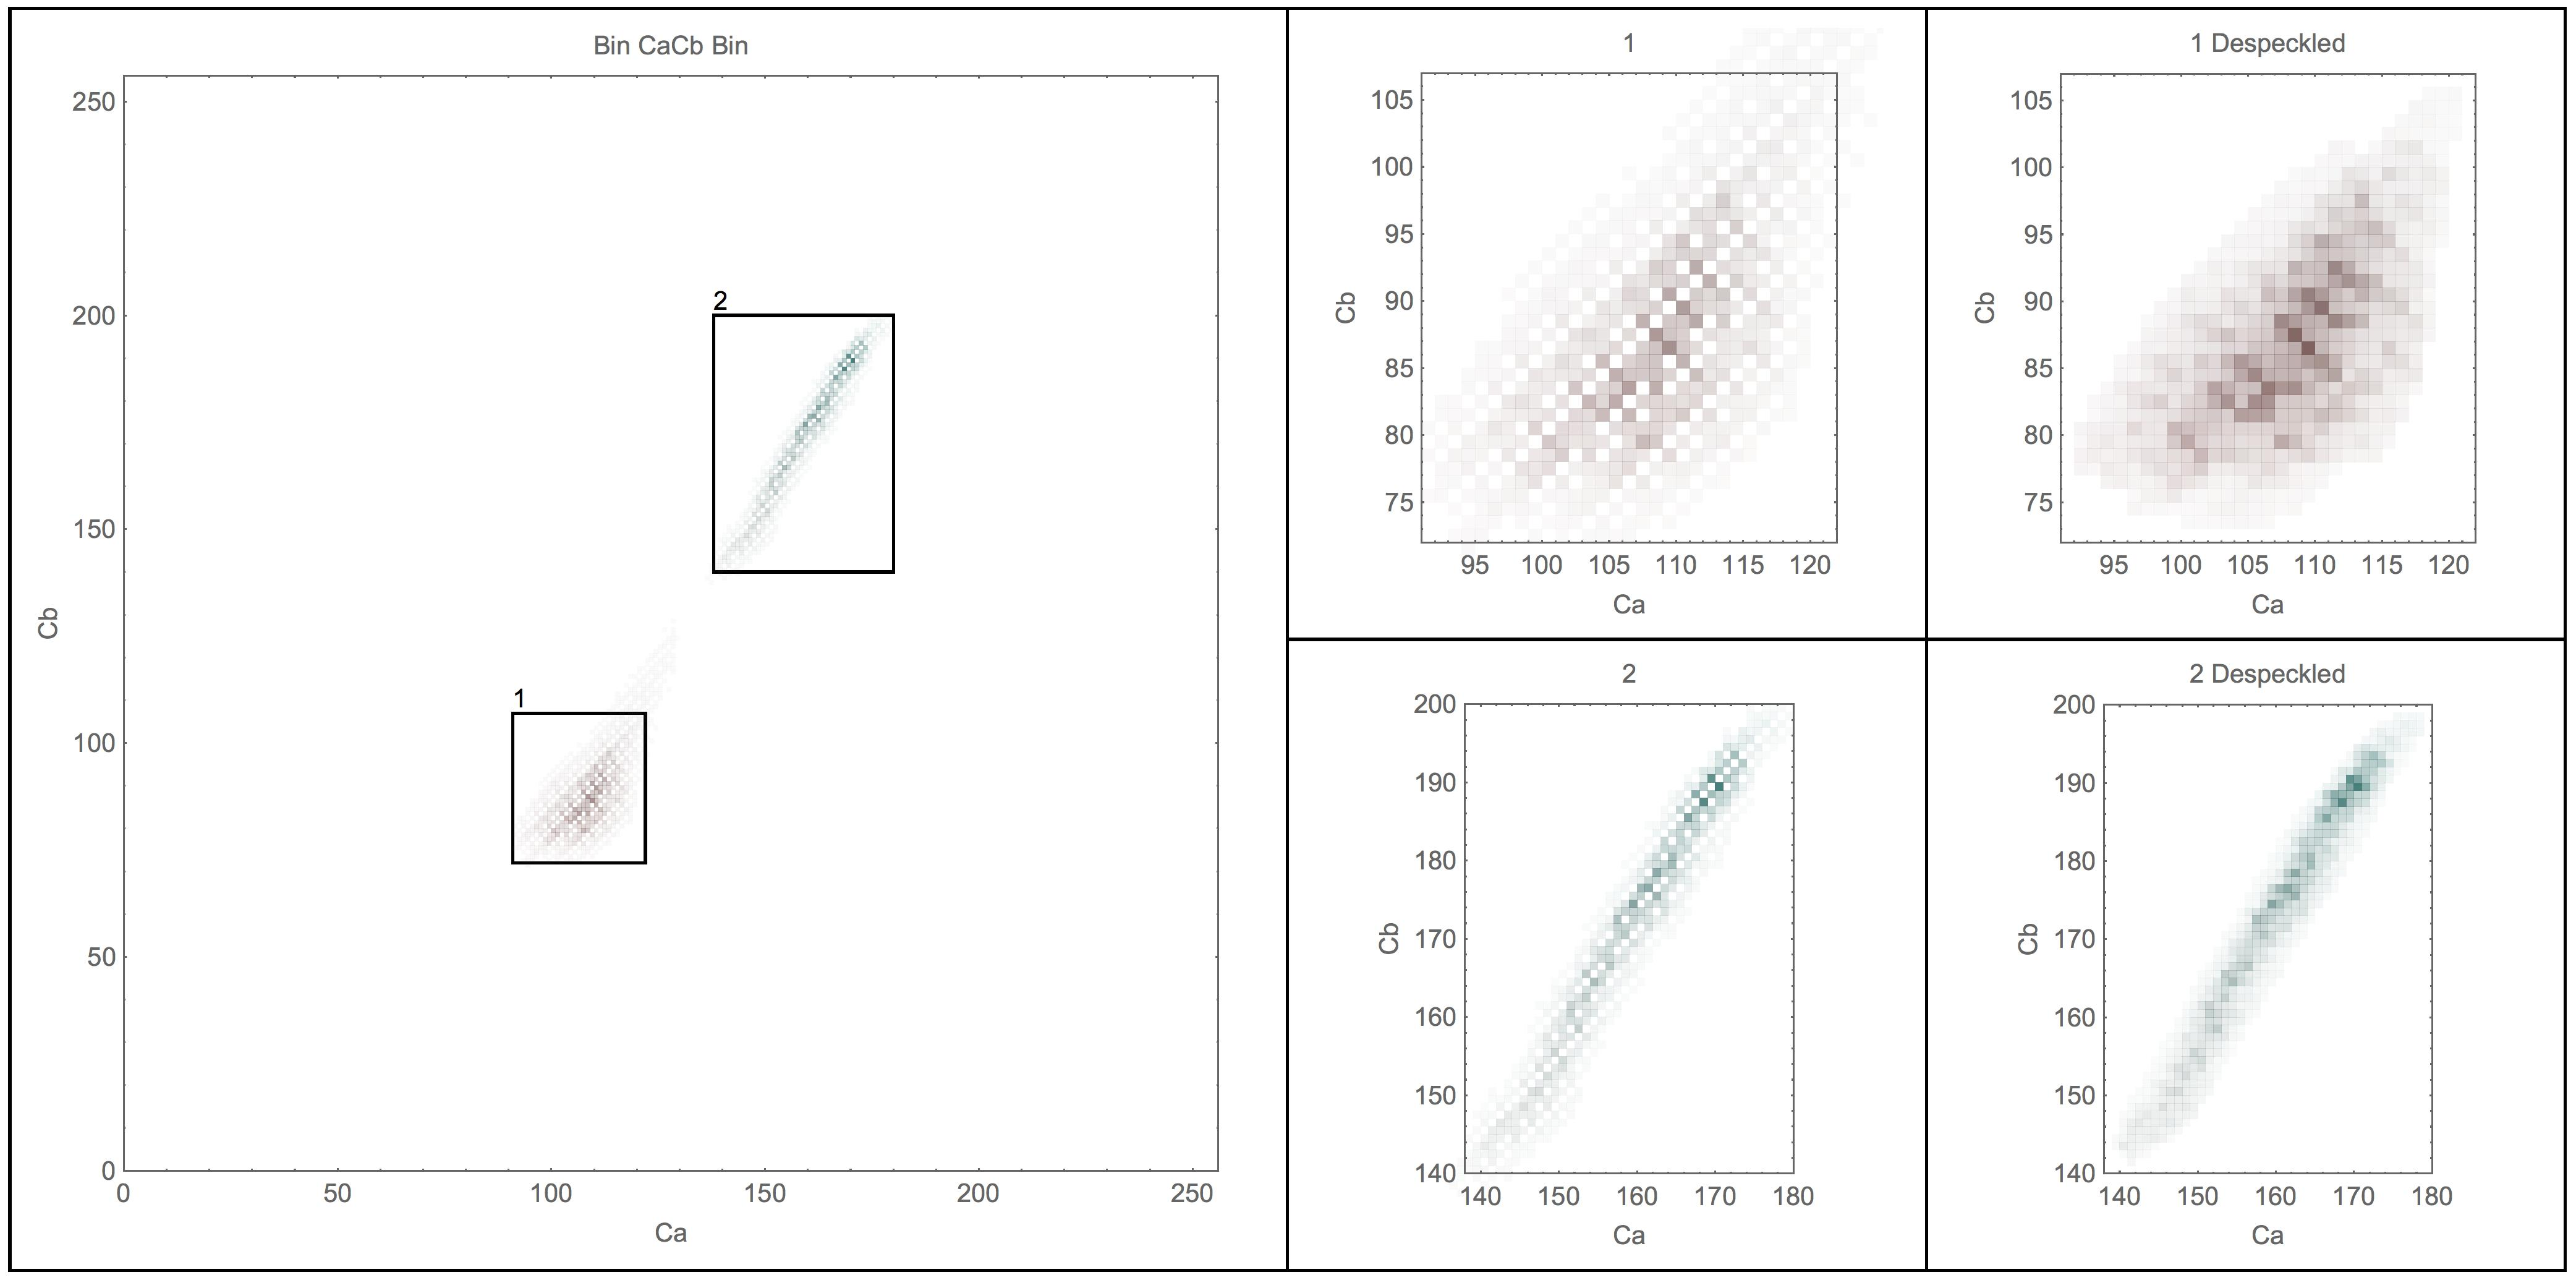
\includegraphics[width=1.0\textwidth]{Chapter3/Figs/\individual/Despeckle_the_Bins.jpg}
        \caption{\textbf{The De-speckled Bins}. The action of the de-speckling algorithm can be seen in the right-hand close-up panels}  \label{fig:Despeckle_the_Bins}
    \end{figure}
    
The raw camera output has, by this stage, undergone two rounds of processing --- first in the device, before the AP layer, creating an 8-bit RGB image; and then in the rotation to the LCaCb space. These processes are, unfortunately, not $1\rightarrow 1$. This results in some bins being artificially overpopulated and other bins becoming artificially empty. The effect of the LCaCb rotation can be controlled by extending the axis lengths; this process can make for at worst $1\rightarrow 1$ correspondence. However, this necessarily introduces a greater number of inaccessible bins. In terms of collecting the statistics, these effects are not problematic aside from the fact that it introduces empty bins inside the main region of interest, which causes difficulties for the algorithm further down the line. Graphically, this problem looks like speckling. This speckling is also apparent in the RGB bins, and so is a result of the pre-processing of the image by the device before the AP layer. It is noteworthy that although the camera claims to capture full 3-channel, 8-bit RGB information, this is not quite true. 

In attempting to solve this problem, the obvious idea is to find all the non-zero bins and fit an interpolating function between them. This will effectively remove the empty bin artefacts within the densely-packed region which is the distribution we're interested in. However, the empty bins outside the main distribution are not artefacts and are genuinely empty bins, so removing all the empty bins and then fitting the function joins together any outlying points or secondary distributions corresponding to regions such as the background. We therefore desire a method which will allow us to keep all the non-empty bins and the empty bins outside the main distribution, i.e. all the genuinely empty bins. To achieve this, we designed a MATLAB routine which essentially paints a region around each non-zero point, marking it as part of the main distribution. It then takes all the unmarked regions and includes all the empty bins in those regions. So, the set of points which is all the non-empty bins and all the empty bins in the unmarked regions satisfies the requirement, and a simple interpolating function can easily be fitted to those points.





\subsection{Blob Detection}\label{sec:BlobDetection}

\begin{figure}[h!]
  \centering
    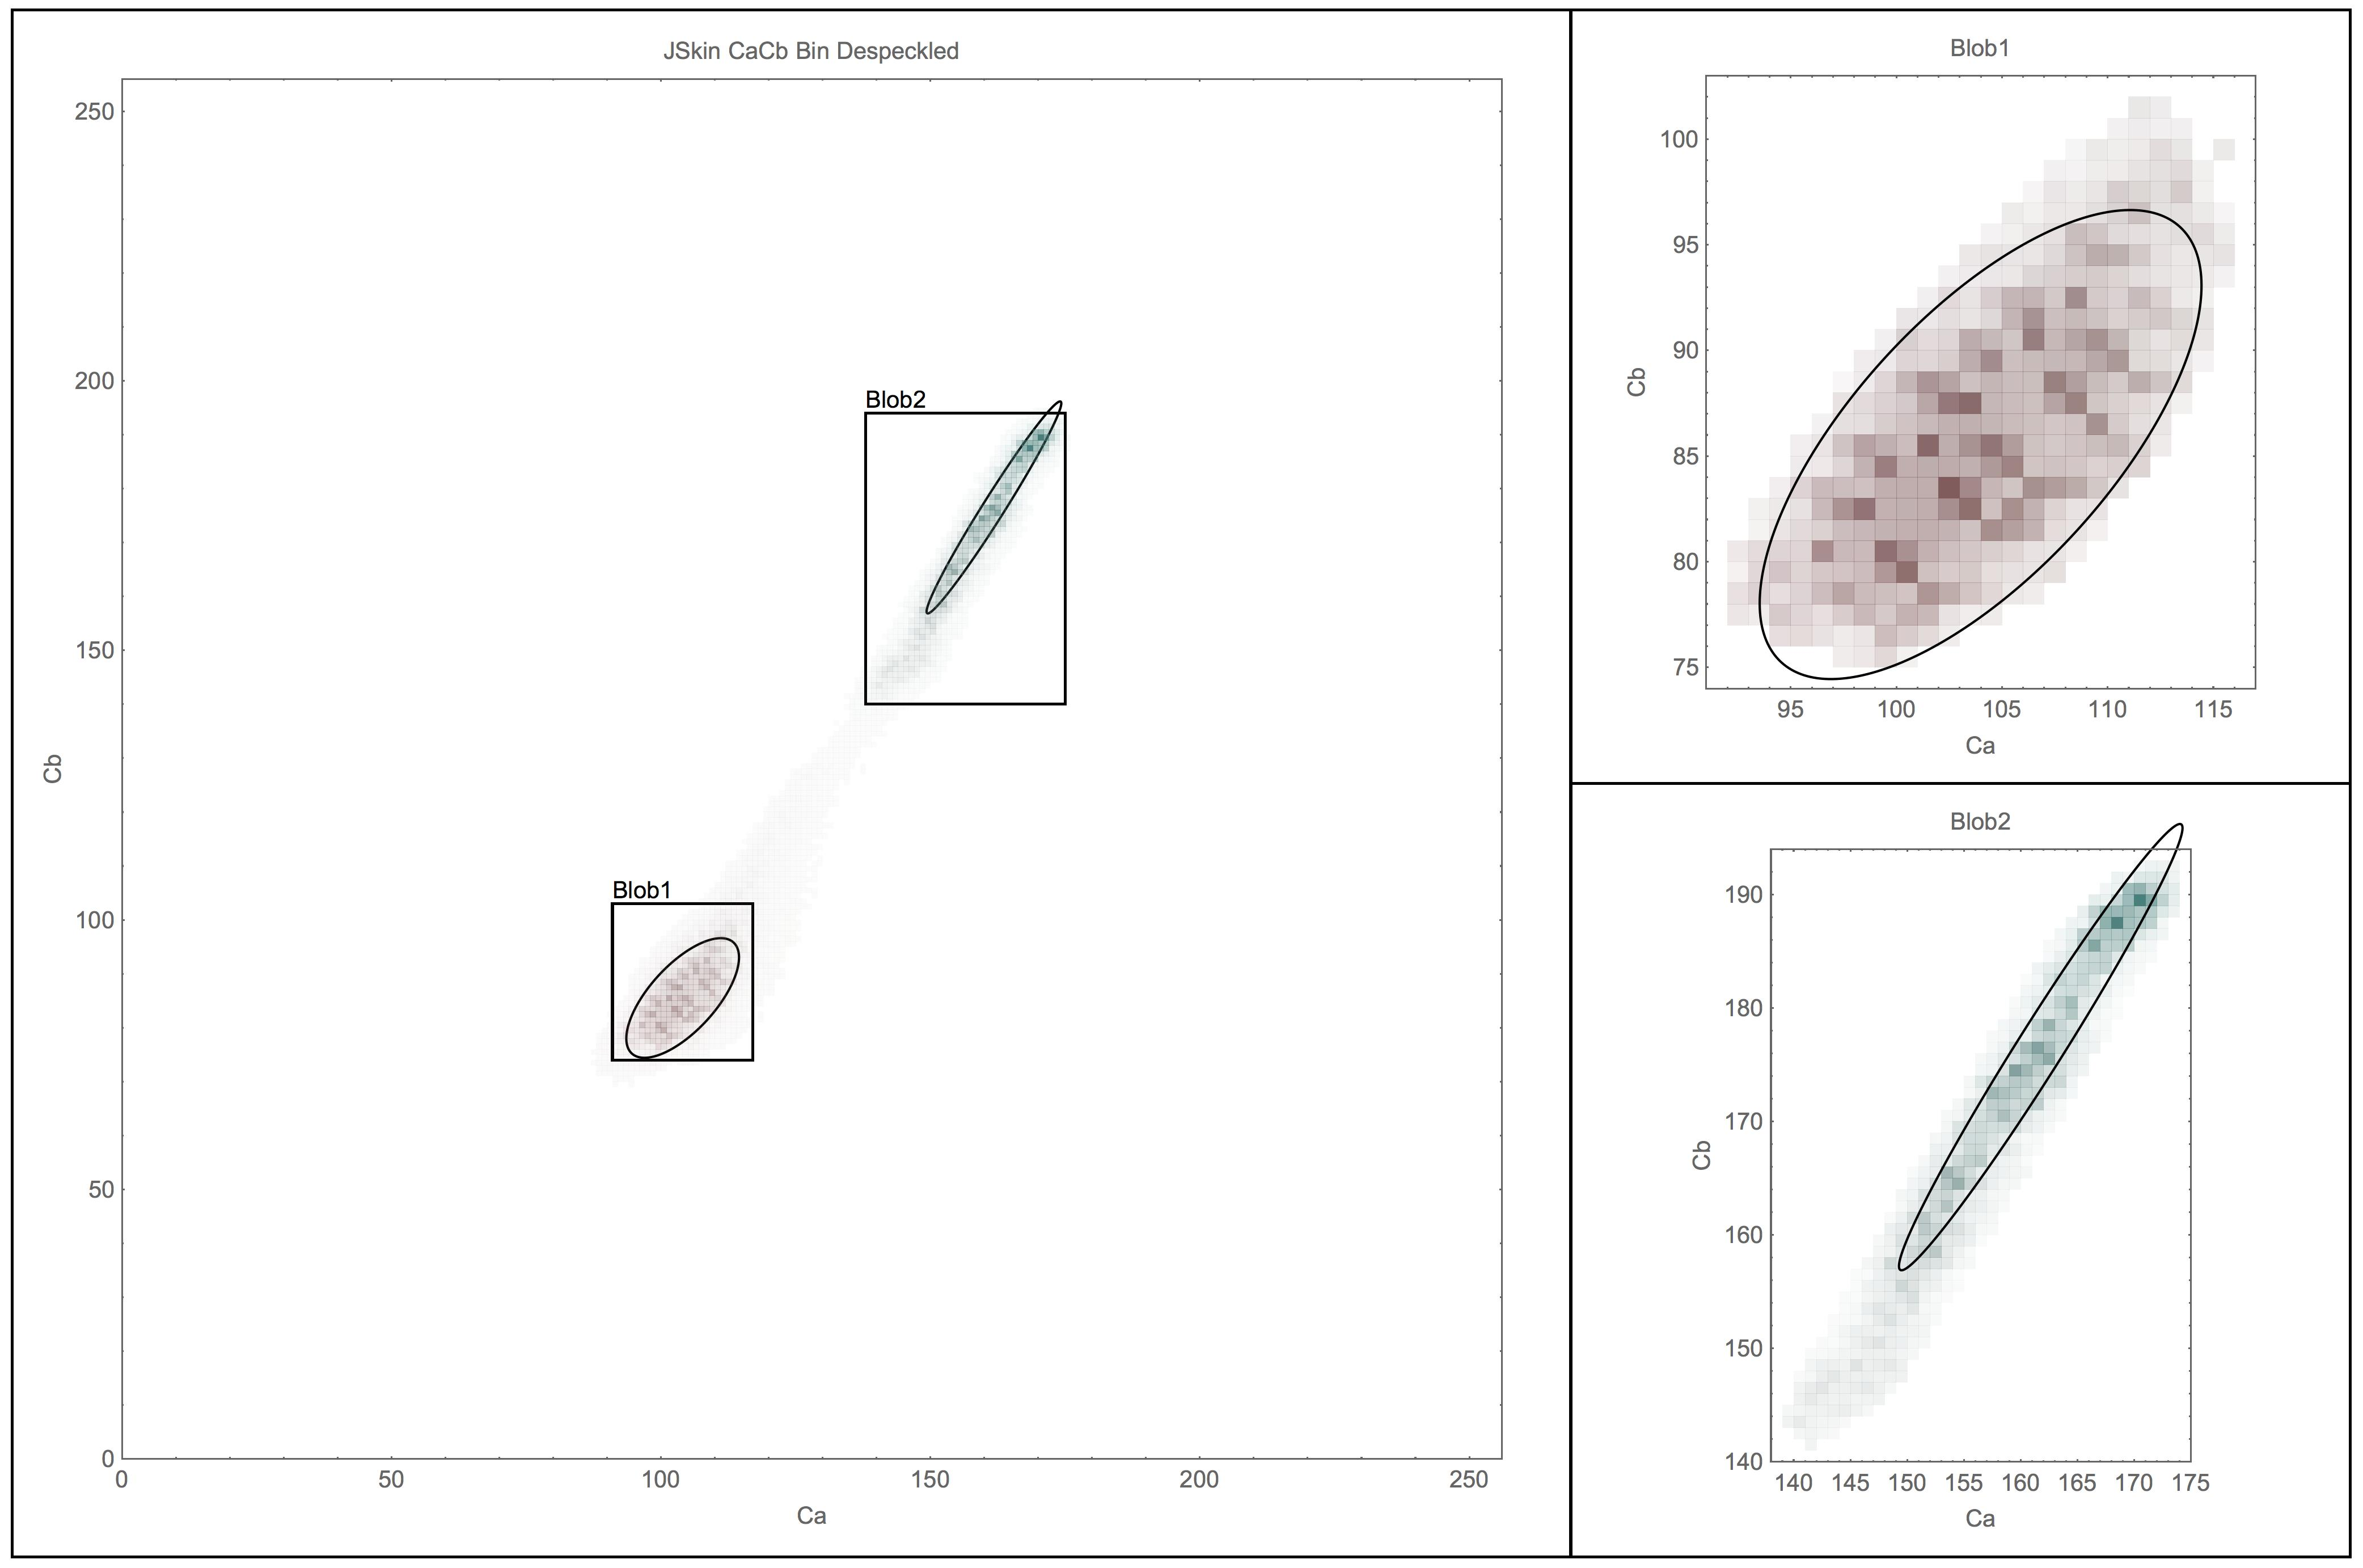
\includegraphics[width=1.0\textwidth]{Chapter3/Figs/\individual/Find_the_Blobs.jpg}
        \caption{\textbf{The Blob Detection.} The detected blobs can be seen in the right-hand panel with the ellipse fit overlayed. The split does not depend on the ellipse but on the extreme edges of the blob.} \label{fig:Find_the_Blobs}
    \end{figure}
    
Having removed the empty bin artefacts and compensated for white-out/black-out effects, the final step is to remove the bin counts of the bins which are associated with the background, thereby leaving a distribution which corresponds to chromatic skin values and which is artefact and systematic-error-free. With the chromatic bins processed as they have been so far, it is clear that there is a distinct distribution for the skin and a distinct distribution for the background.

Using MATLAB's blob detection algorithm, we can find the distinct patches of chromatic information. We expect there to be two distinct blobs: one corresponding to the target skin values, and one to the monochromatic background. The distribution is divided into two, one for each of the detected blobs (Figure \ref{fig:Find_the_Blobs}). The blob detection algorithm also returns the center $\widetilde{\mu}$, eccentricity $\widetilde{\theta}$ and major and minor axis $\widetilde{\sigma}$ for an ellipse which most closely fits the blob shape. The distribution which contains the blob center closest to a reference skin value is chosen to be the skin distribution and the ellipse values are passed to the next step where the Gaussian fit is obtained. Only the bin values between the extreme edges of the blob are passed on to the next stage.

\subsection{The Gaussian Fit}\label{sec:TheGaussianFit}

\begin{figure}[h!] %hi-res
  \centering
    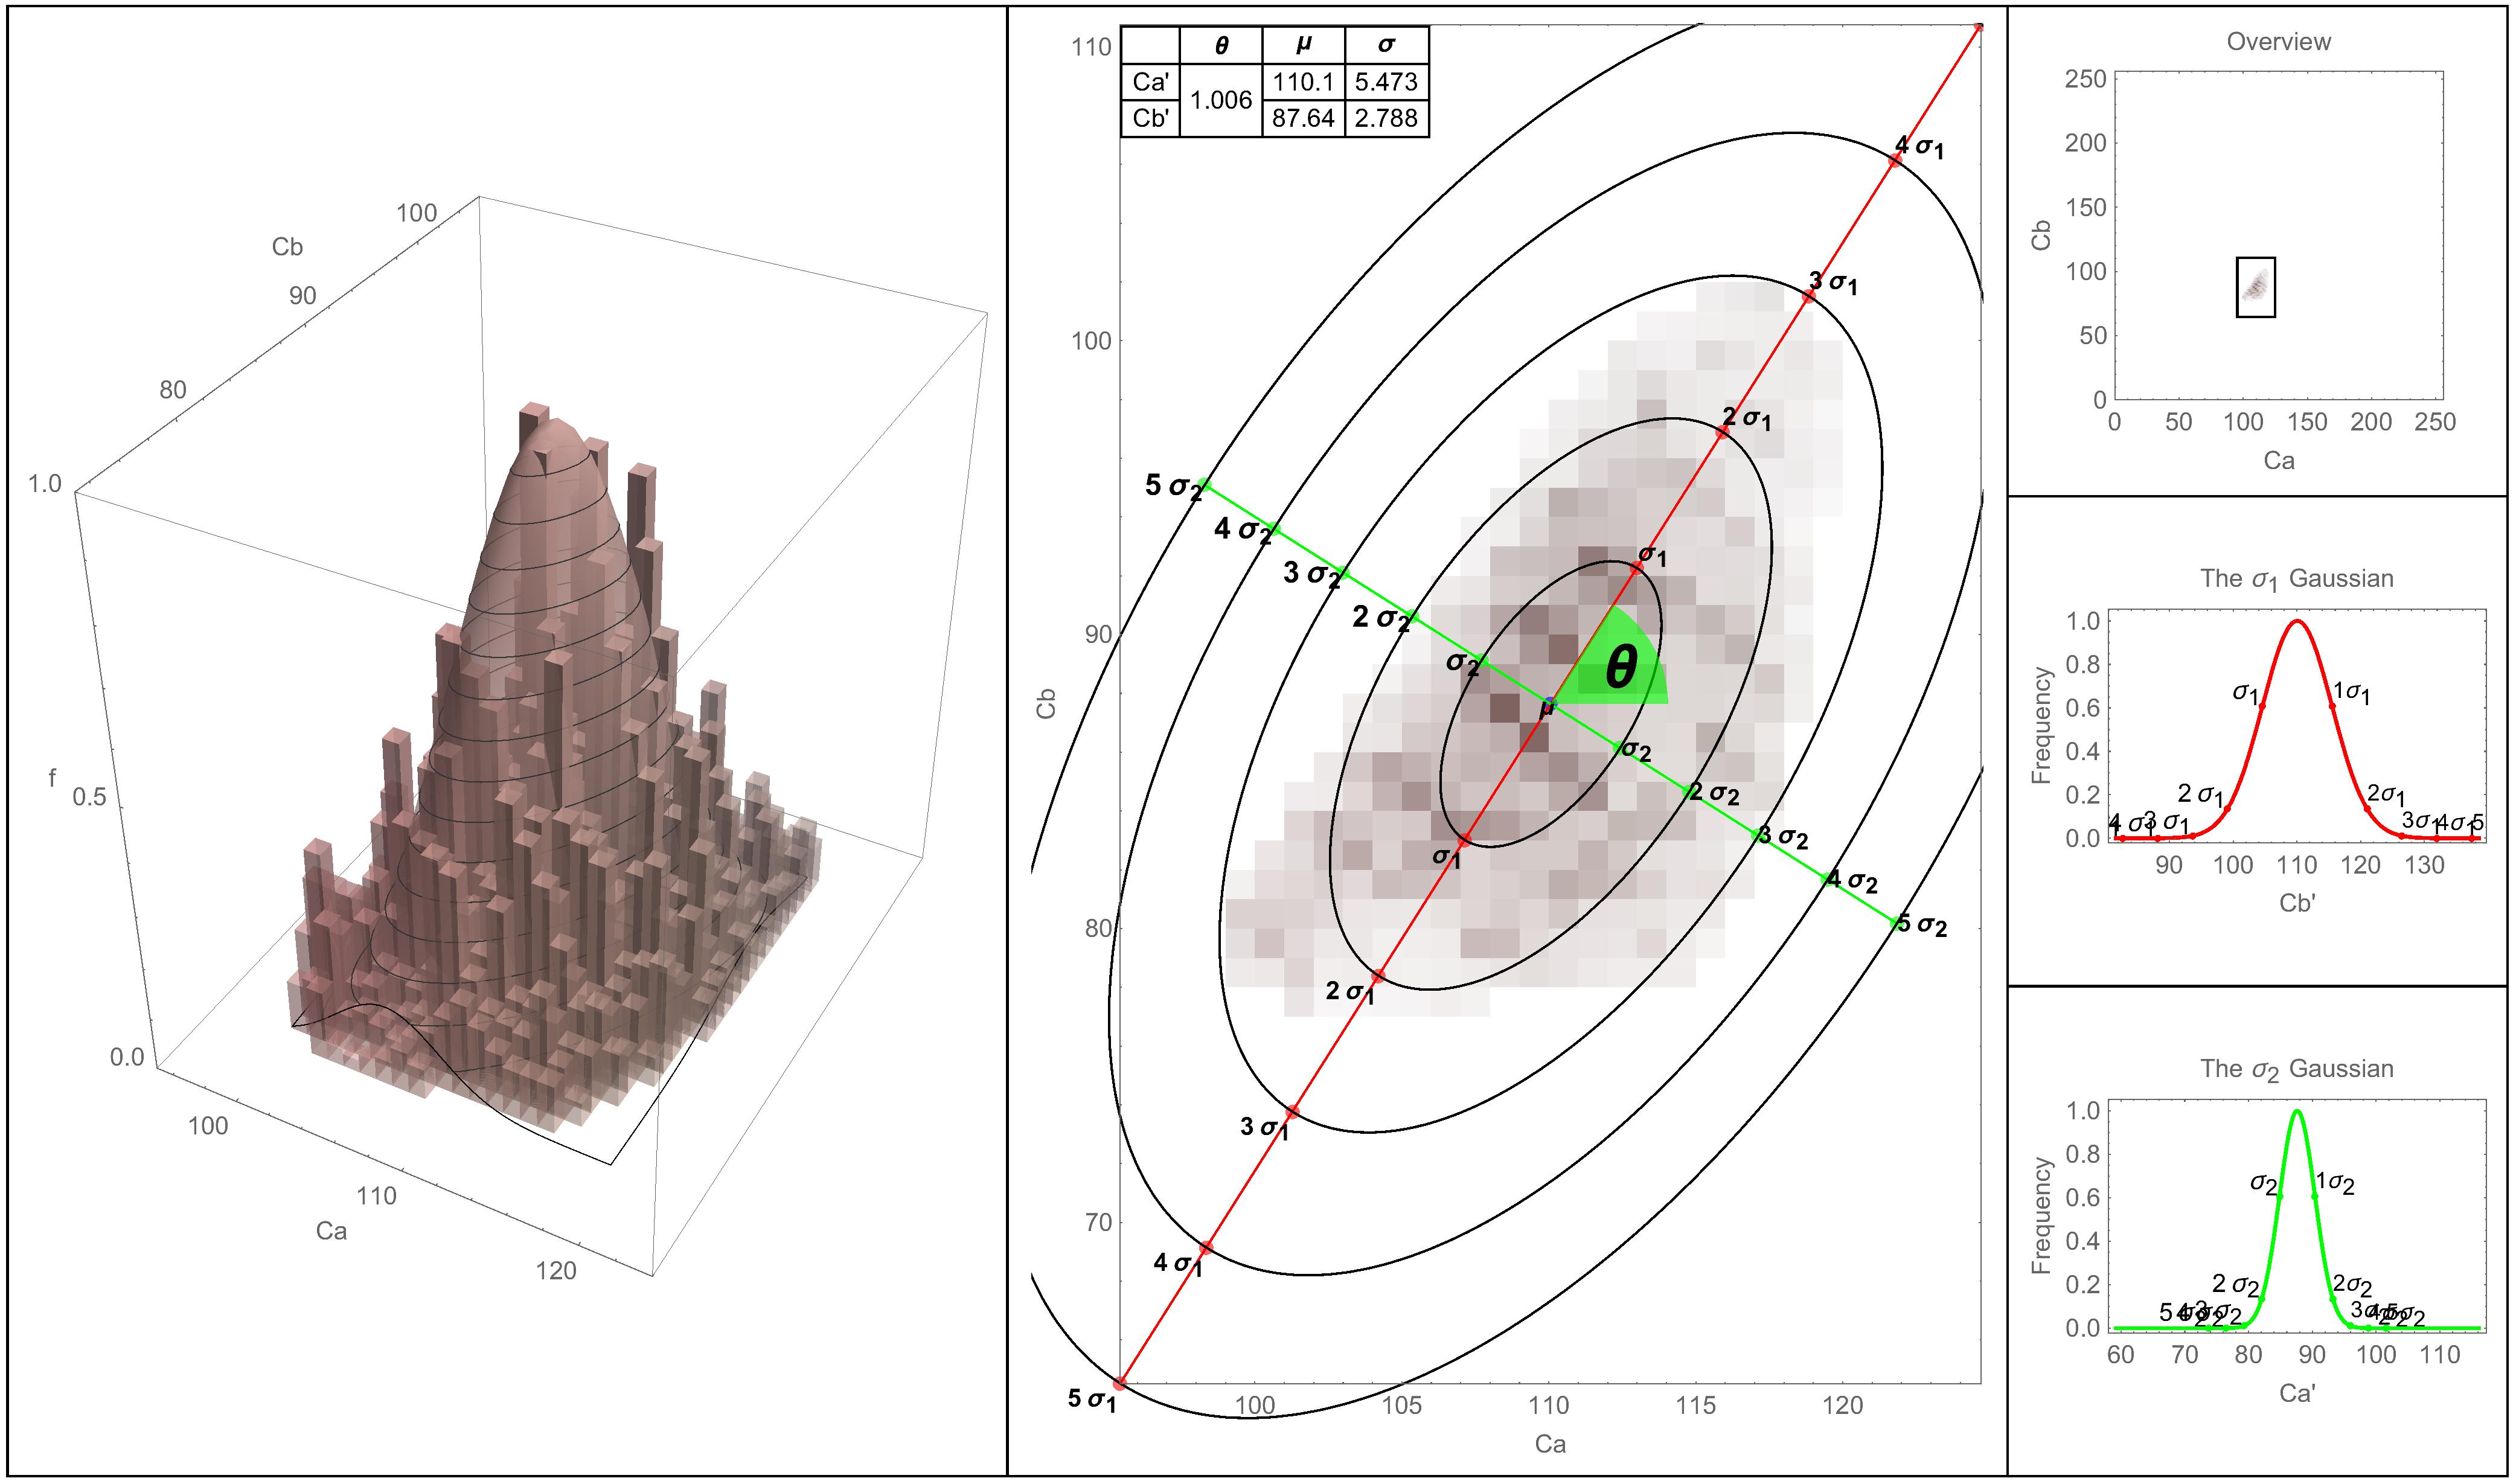
\includegraphics[width=1.0\textwidth]{Chapter3/Figs/\individual/Fit_the_Gaussian0.jpg}
        \caption{The Gaussian fit to the blob}  \label{fig:Fit_the_Gaussian0}
    \end{figure}


We now have a histogram which has bin values relevant to the target and no others. The elliptical blob fit values are used to initialize a 2D Gaussian fit to the normalized histogram. 

A least squares fit of the 2D Histogram with a 2D Gaussian function (Equation \ref{eq:2DGaussian}) is found using MATLAB's lsqcurvefit function.
\newcommand{\CaMu}{ \overline{\mathbf{Ca}} }
\newcommand{\CbMu}{\overline{\mathbf{Cb}}  }
\begin{gather}\label{eq:2DGaussian}
\textbf{Let} \quad \CaMu = \text{Ca}-\mu_1 \quad \text{and} \quad \CbMu = \text{Cb}-\mu_2 \\
\exp \left(
-\frac{\left( - \CaMu \; \sine{     \theta } + \CbMu \; \cosine{ \theta } \right){}^2}{2 \sigma_2^2} - 
\frac{\left(      \CaMu \; \cosine{ \theta } + \CbMu \; \sine{      \theta} \right){}^2}{2 \sigma_1^2} \right)
\end{gather}



\section{Sample Sets and Results}\label{sec:SampleSets}

\begin{figure}[h!]
  \centering
    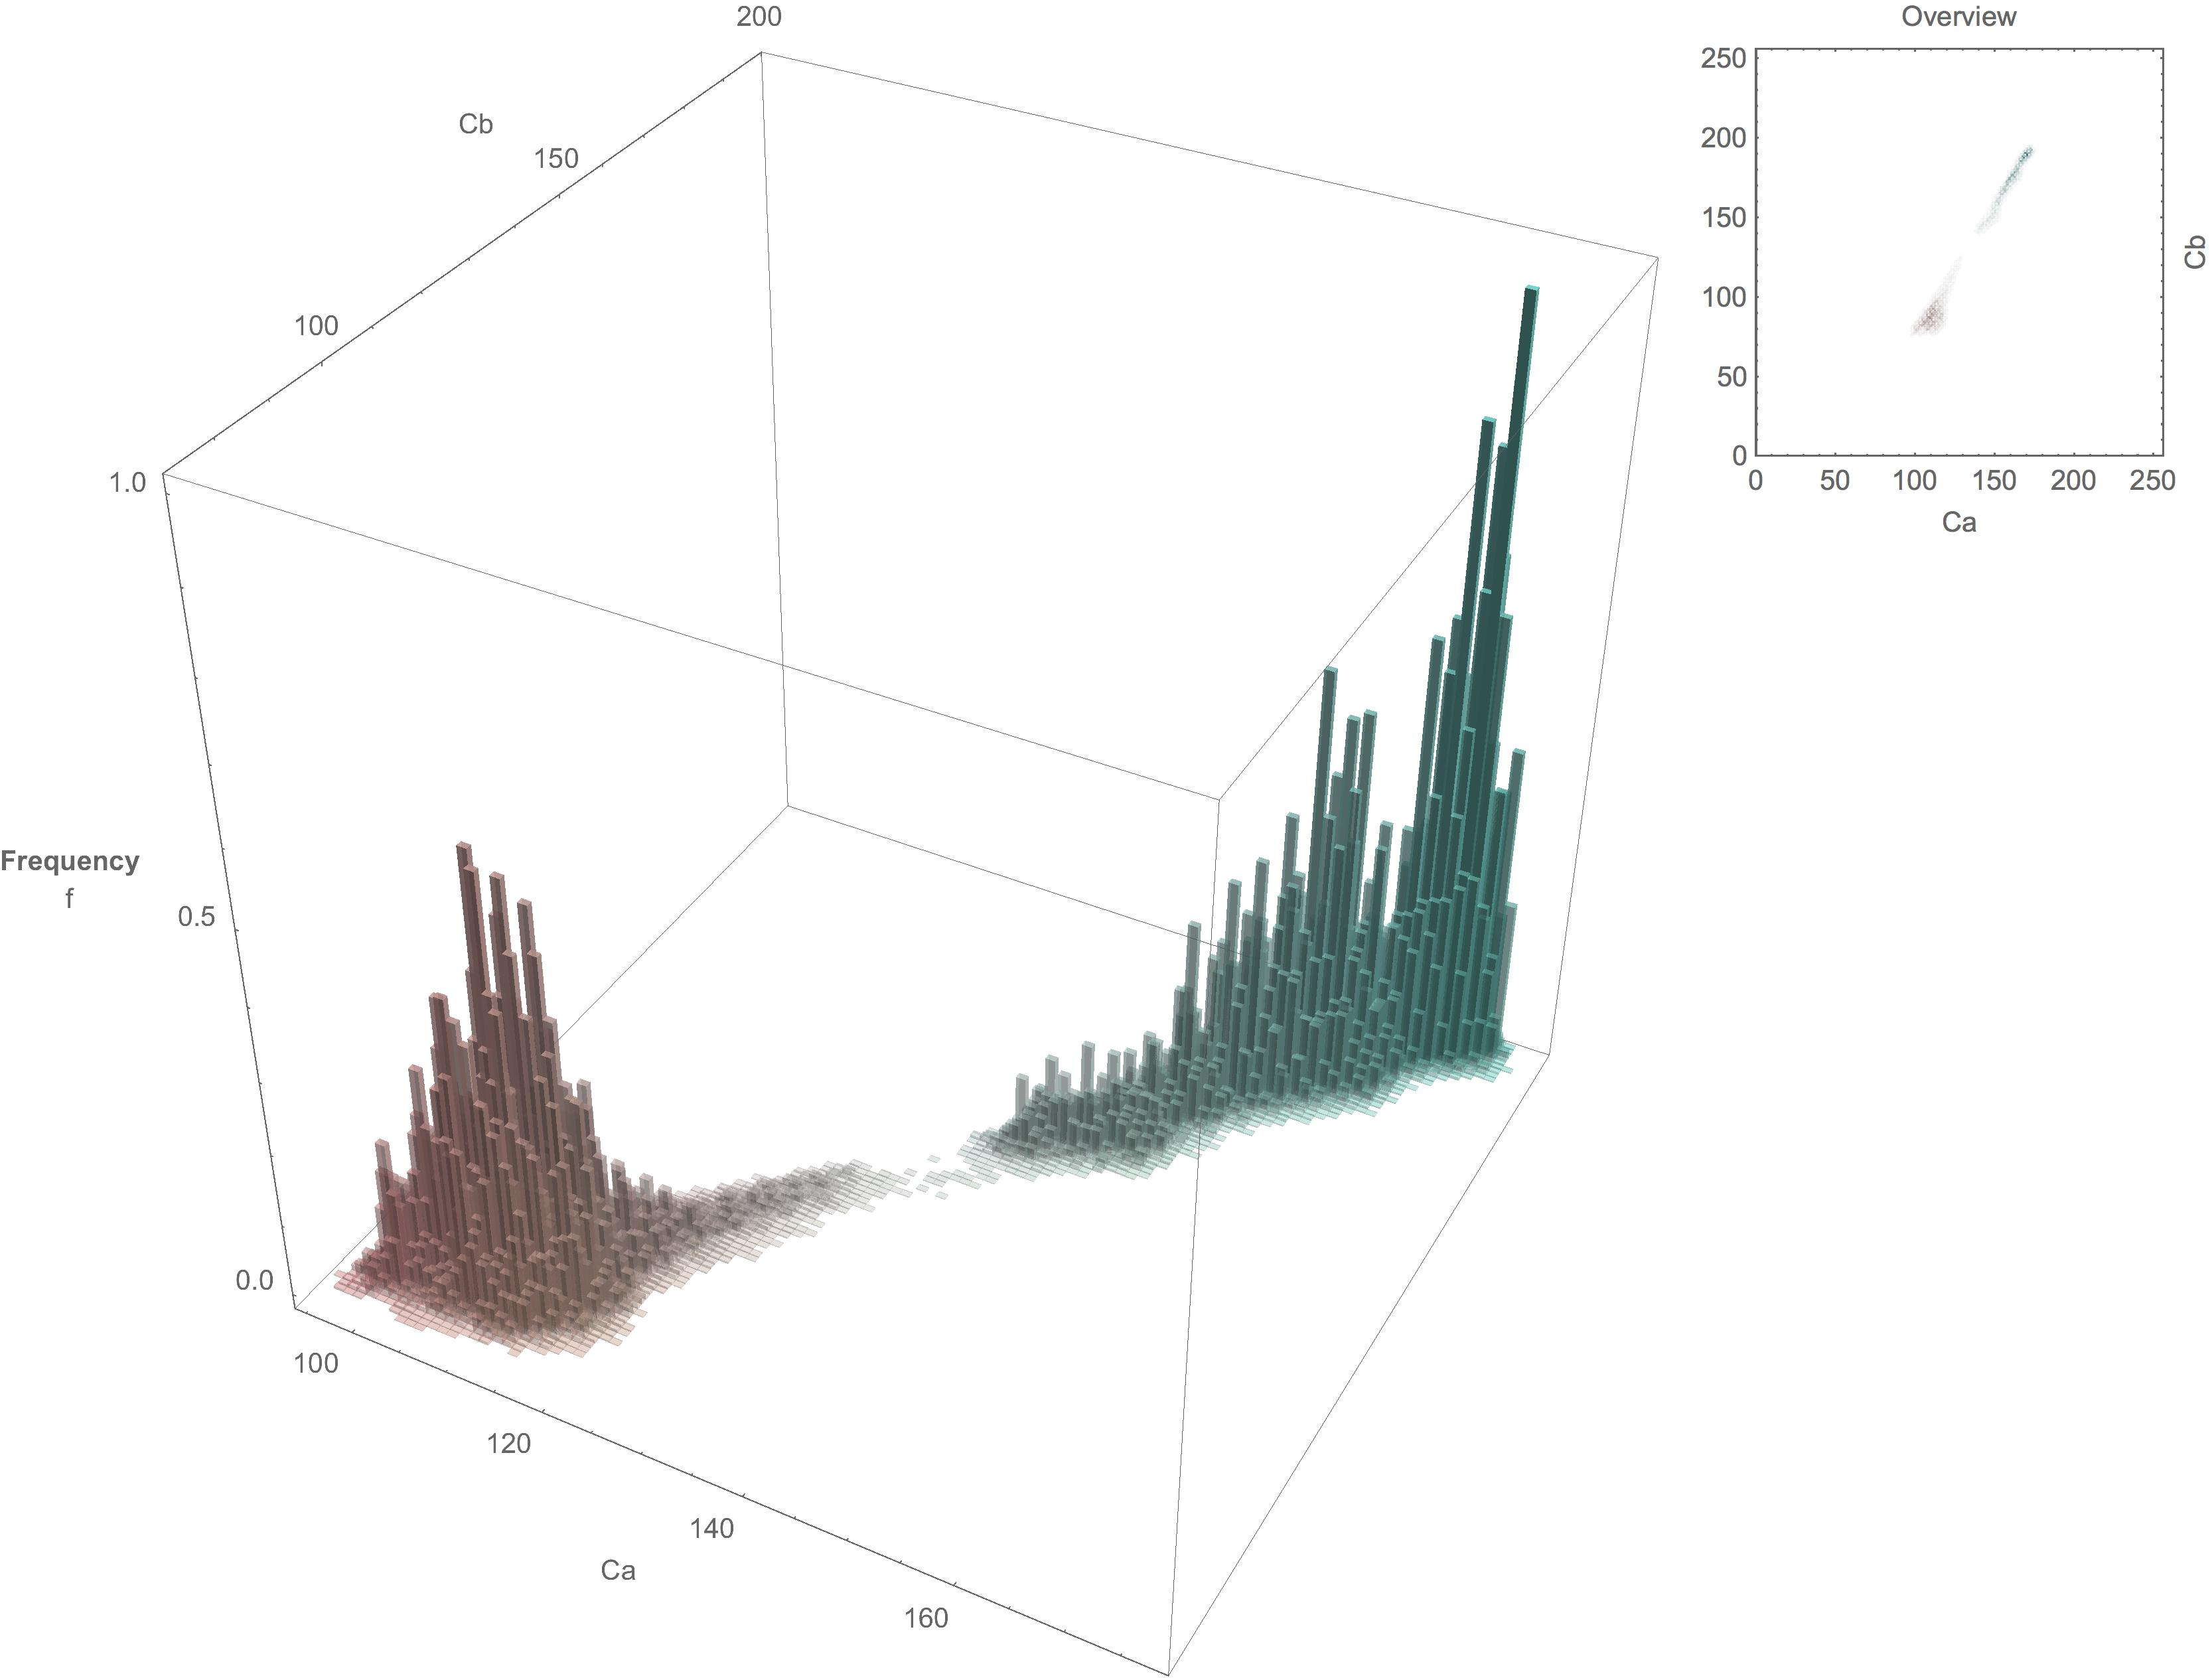
\includegraphics[width=1.0\textwidth]{Chapter3/Figs/\individual/Despeckle_the_Bins_Surf.jpg}
        \caption{The Ca Cb histogram for the combined F,J\&N sets incliding the background. The colors indicate the pixel color corresponding to the bin. }  \label{fig:Despeckle_the_Bins_Surf}
    \end{figure}

\begin{figure}[h!]
  \centering
    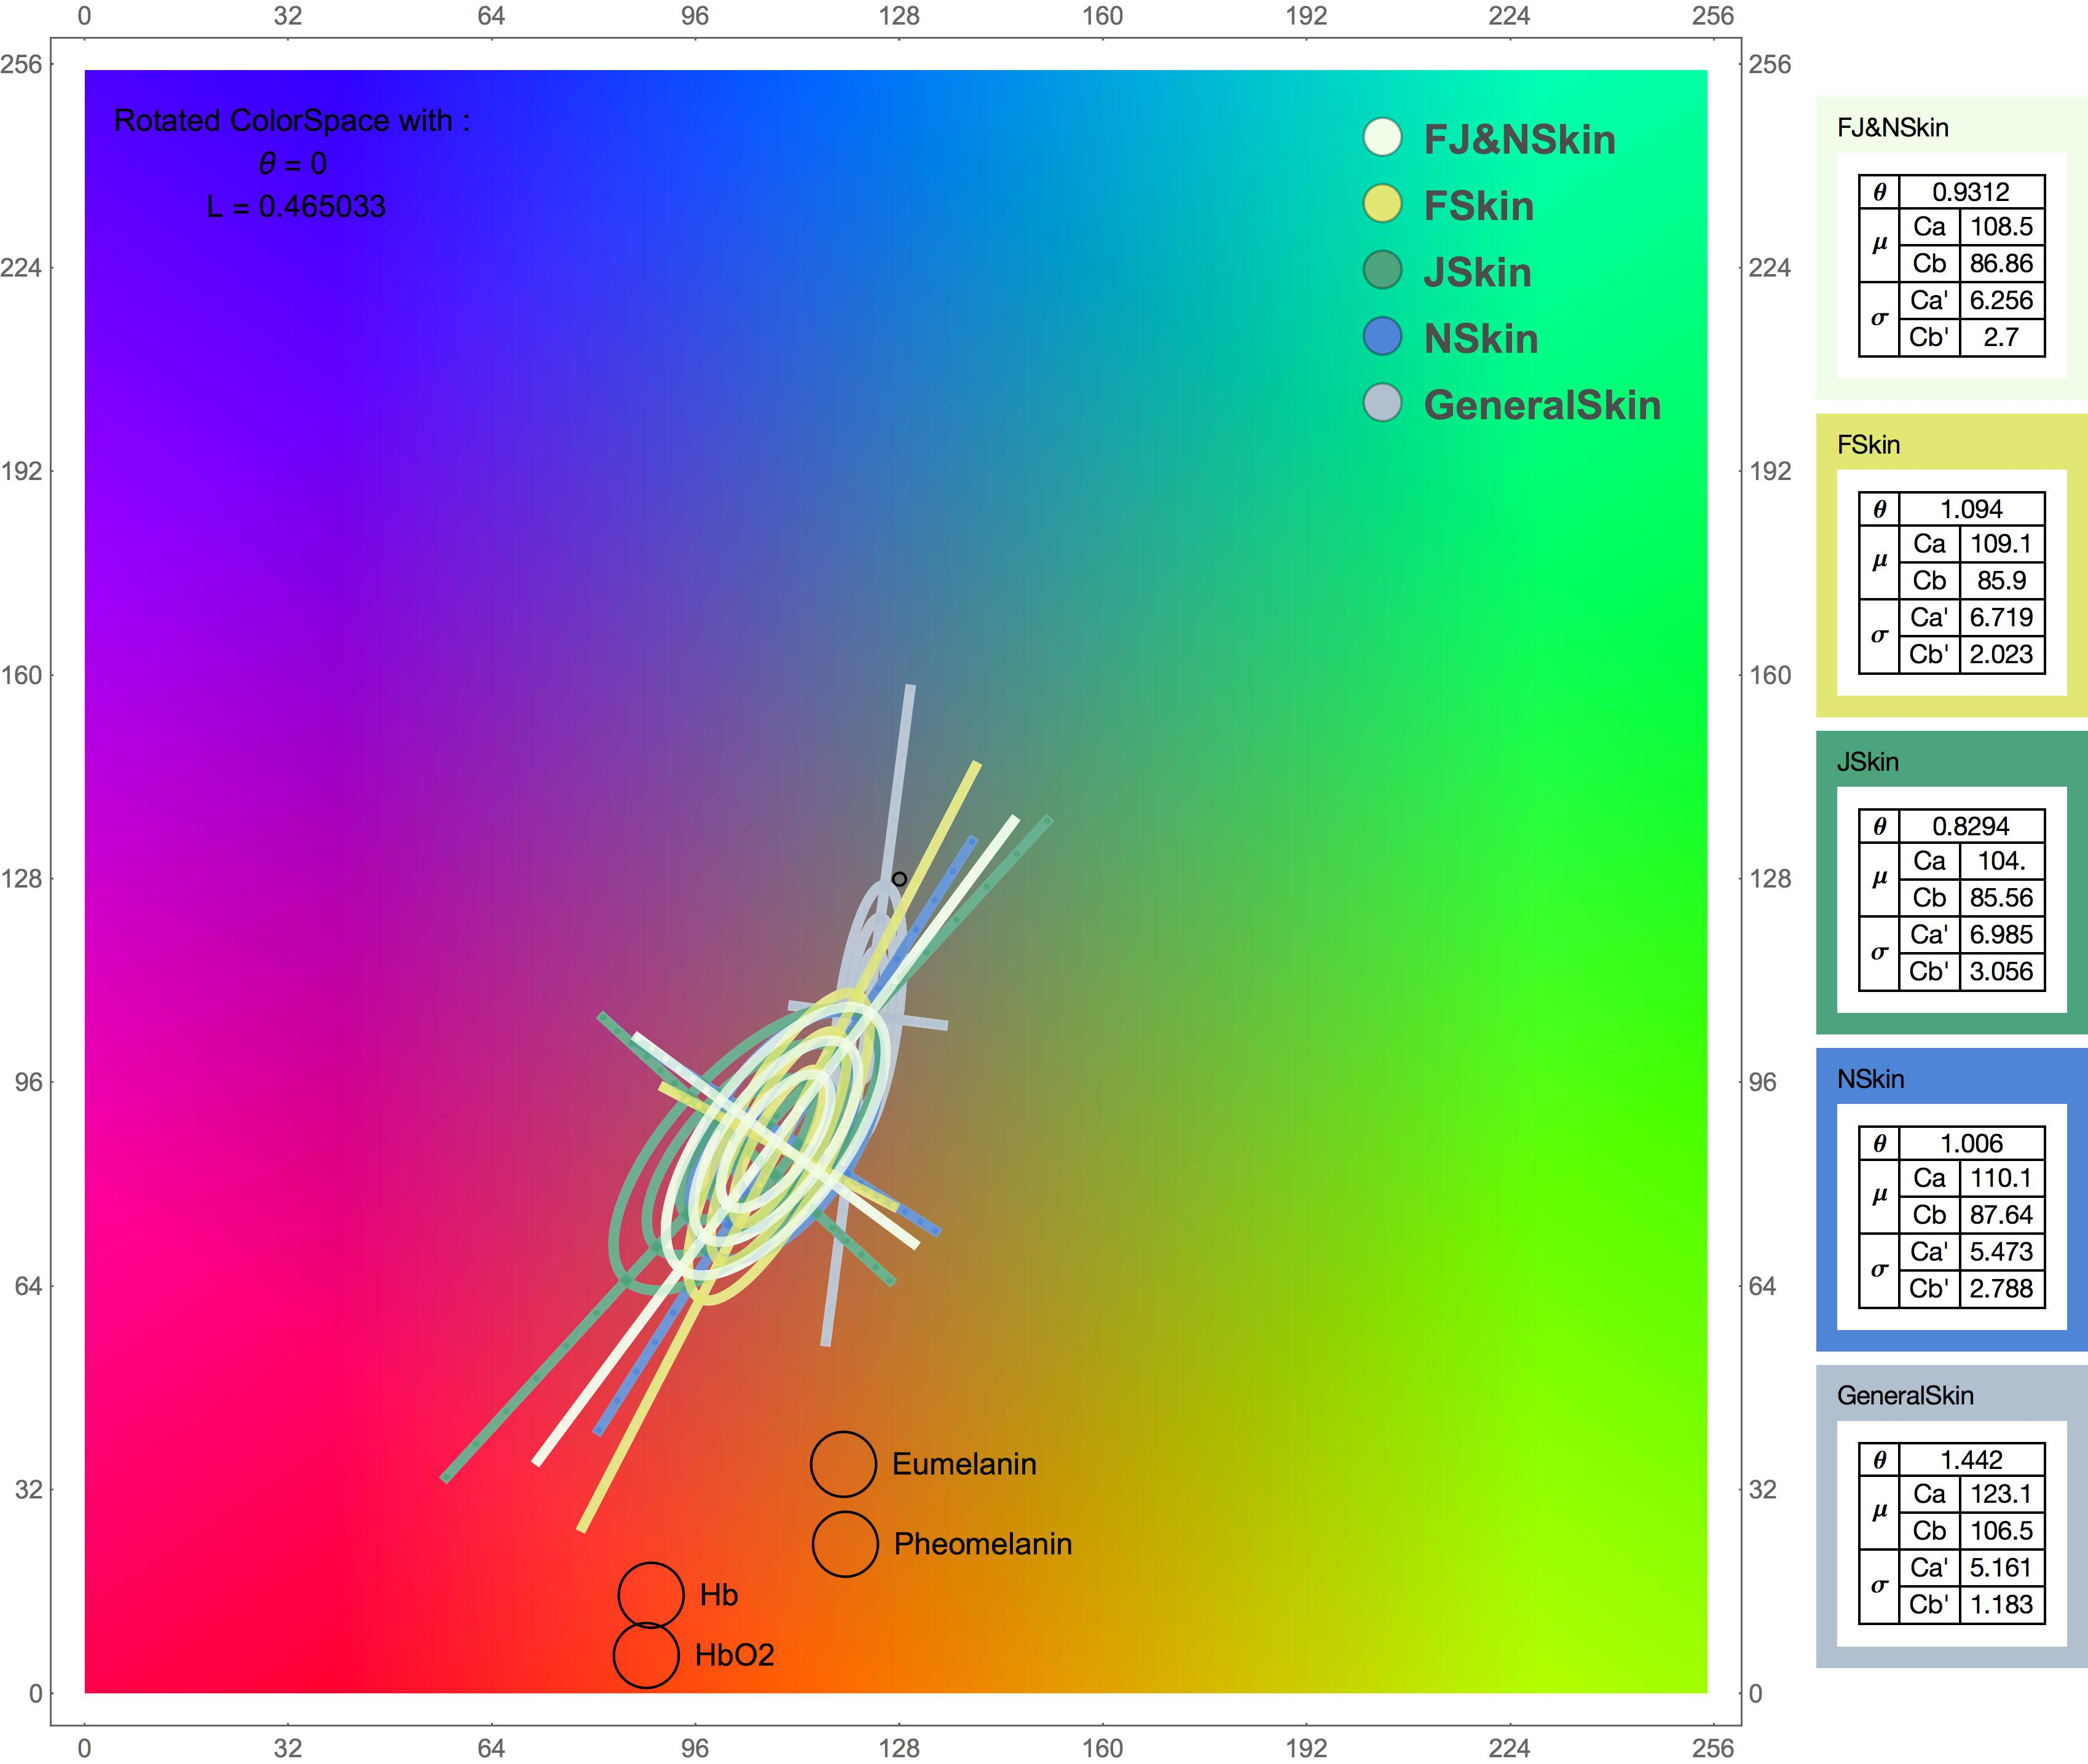
\includegraphics[width=\textwidth]{Chapter3/Figs/All_Together_2D.jpg}
    \caption{The four sets and the combined set of individuals. The ellipses are placed at $2\sigma$, $3\sigma$ and $4\sigma$ positions. Values inside $2\sigma$ would be kept by the distribution function.}  \label{fig:AllTogether2D}
\end{figure}


\begin{figure}[h!]
  \centering
    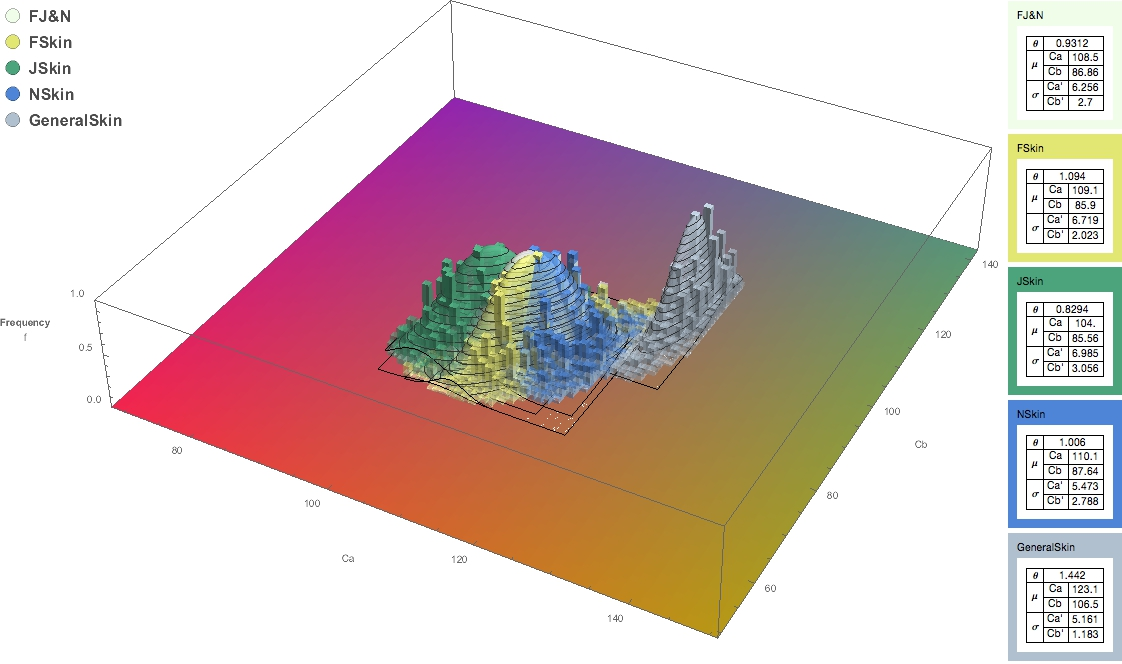
\includegraphics[width=\textwidth]{Chapter3/Figs/All_Together_3D.jpg}
    \caption{The histograms for the four data sets and the combined set of individuals are shown alongwith the Gaussian fits to the histogram. The color indicates the data set.}  \label{fig:AllTogether3D}
\end{figure}

Sample image sets were collected using the iPhone for three individuals with varying skin tones. Sets of images were taken for each digit and the hand as a whole under different lighting conditions and orientations. A selection of the images can be seen in Figure \ref{fig:SetSamples}


\begin{figure}[h!]
  \centering
  \begin{tabular}{||c||c||c||}
  \hline \rule[-2ex]{0pt}{5.5ex}  FSkin &  JSkin & NSkin \\ 
  \hline \rule[-2ex]{0pt}{5.5ex} 
  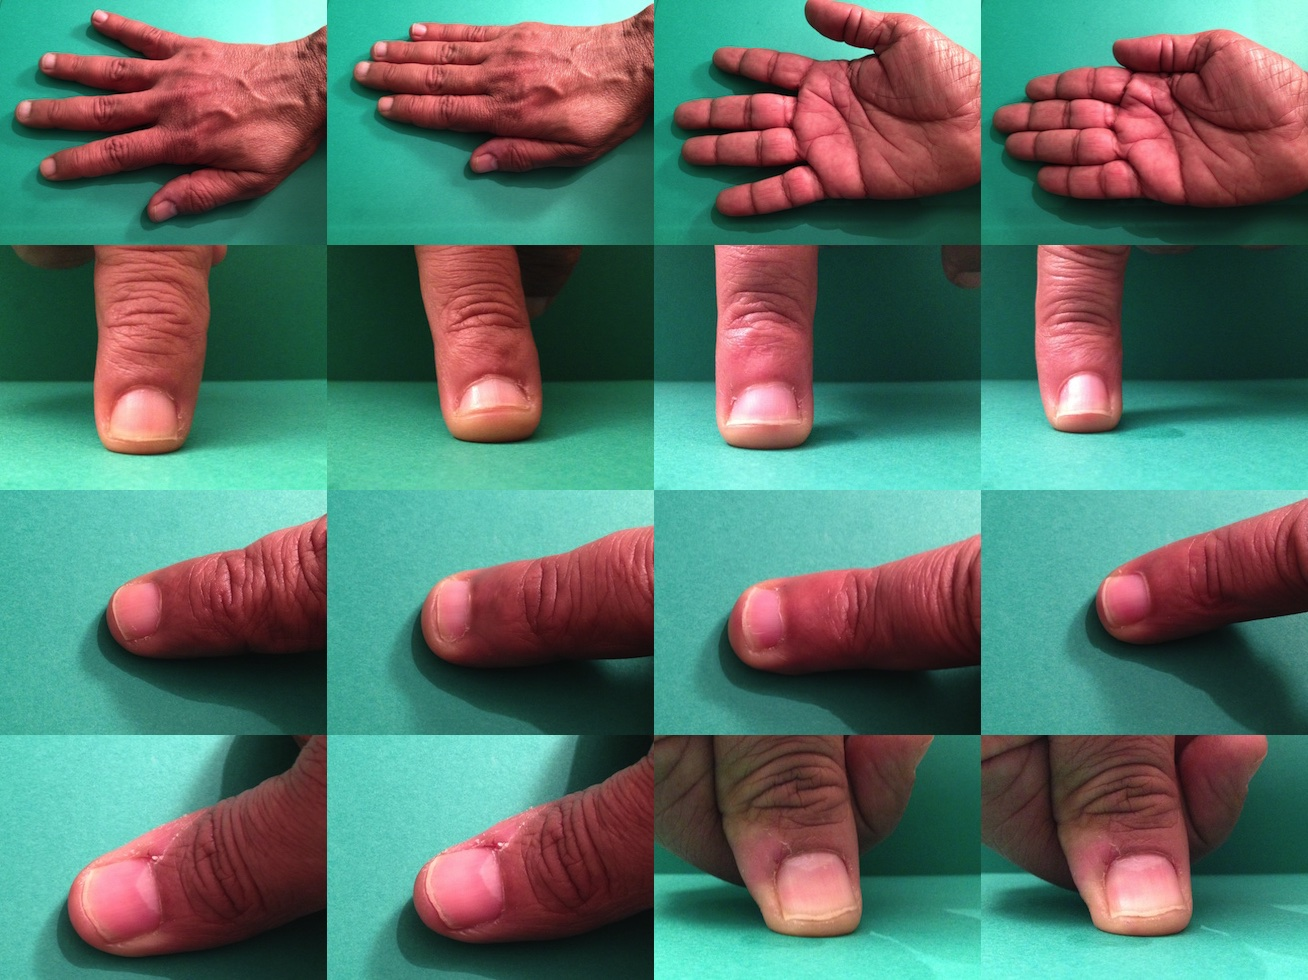
\includegraphics[width=0.3 \textwidth]{Chapter3/Figs/SampleCollages/FSkin_Sample.jpg} & 
  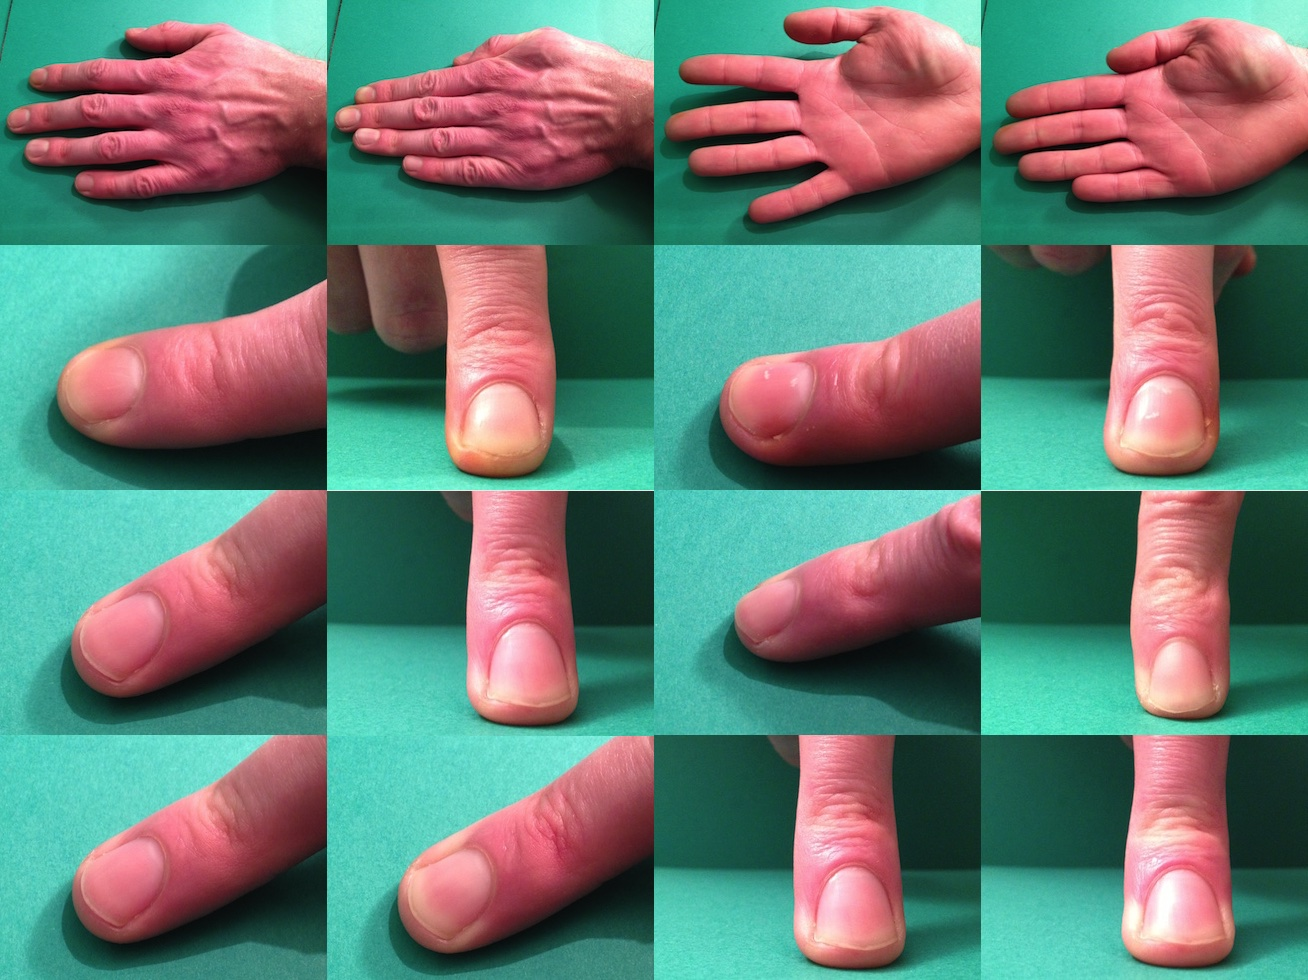
\includegraphics[width=0.3 \textwidth]{Chapter3/Figs/SampleCollages/JSkin_Sample.jpg} &  
  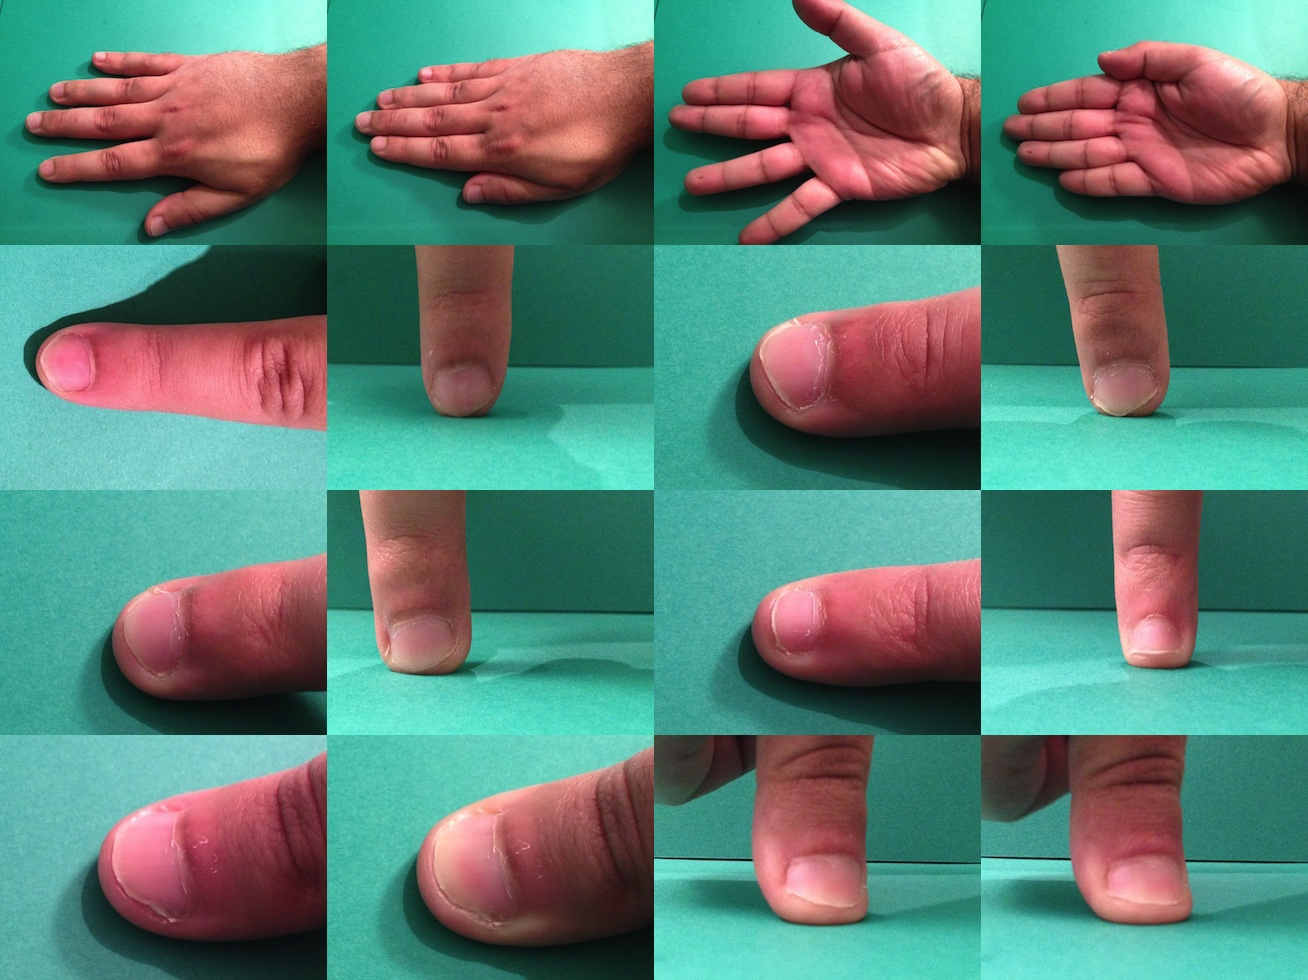
\includegraphics[width=0.3 \textwidth]{Chapter3/Figs/SampleCollages/NSkin_Sample.jpg}\\ 
  \hline 
  \end{tabular} 
    \caption{Samples from the image sets for each individual.}  \label{fig:SetSamples}
\end{figure}

The MATLAB bin class was written so that the combined statistics for the three individuals could be found by adding the RGB bins together, and then following the same steps 1-8 as described previously. All three distributions along with the combined distribution can be seen in Figures \ref{fig:AllTogether2D} and \ref{fig:AllTogether3D}.


In an attempt to identify a larger range of values for the skin space, a large number of skin samples were taken from photographs from the Humane project by Angelica Dass, an ongoing "chromatic inventory" art project which aims to compile every possible human skin color, categorized by the PANTONE guide color classification system~(\cite{Dass2012}). The skin colors catalogued thus far are independent of race or ethnicity, so the samples are representative of human skin tones in general.

The image set consists of approximately 200 skin samples  each showing only one individuals skin. The result can be seen in Figures \ref{fig:AllTogether2D} and \ref{fig:AllTogether3D} as the GeneralSkin set. The distribution stands apart from the others and surprisingly has a smaller standard deviation. This is probably due to camera differences and the sampling techniques used in the Humane project which focus on finding an average color rather than the channel values in camera. The orientation and position of the distribution is more consistent with the theoretical values for the skin pigments than those for the individual sets. This is likely due to the fact that the theoretical values were calculated for a different camera CCD, the iPhone CCD characteristics not being available. For this reason the general distribution is excluded from further consideration aside from the recognition that different cameras will require bespoke statistics to be gathered. 

In contrast to the GeneralSkin set the individual sets are close together with similar standard deviations however the angle varies significantly. The angle needs to be fixed so that the statistics can be gathered in the rotated color-space. The angles are summarised in the table below:

\begin{tabular}{|c|c|c|c|}
\hline   Set                                                             & Decimal   & Approx                       & Relative \\ 
\hline   $\text{FJ$\&$NSkin }\theta _{\text{FJN}}$ & $0.9312$ & $\frac{75 \pi }{253}$ & $\theta _{\text{FJN}}$ \\
\hline   $\text{FSkin }\theta _F$                            & $1.0940$ & $\frac{39 \pi }{112}$ & $\theta _{\text{FJN}}+\frac{3 \pi }{58}$ \\
\hline   $\text{JSkin }\theta _J$                             & $0.8294$ & $\frac{33 \pi }{125}$ & $\theta _{\text{FJN}}-\frac{\pi }{31}$ \\
\hline   $\text{NSkin }\theta _N$                          & $1.0060$ & $\frac{49 \pi }{153}$ & $\theta _{\text{FJN}}+\frac{\pi }{42} $\\
\hline 
\end{tabular} 

This suggests that taking $\theta'$ to be in the range $\theta _{\text{FJN}} -\frac{\pi}{84} < \theta' < \theta _{\text{FJN}} +\frac{\pi}{84}$ is safe as it is at most half way to the nearest individual and the position of the mean remains within 2 standard deviations 
$\left(\begin{array}{c} 84 \\ 117 \end{array} \right) < \mu'  < \left(\begin{array}{c} 83 \\ 121 \end{array} \right) $. This is somewhat arbitrary and we could extend the region if we had reason but this range is sufficient to ensure that a computationally advantageous value will be within the range being 1/7 th of a Pi/6 region.  The perturbation to the channels for the range of possible $\theta'$ values can be seen in Figures \ref{fig:PerturbationNearThetaAB} and \ref{fig:PerturbationNearThetaT}.


\begin{figure}[h!]
  \centering
  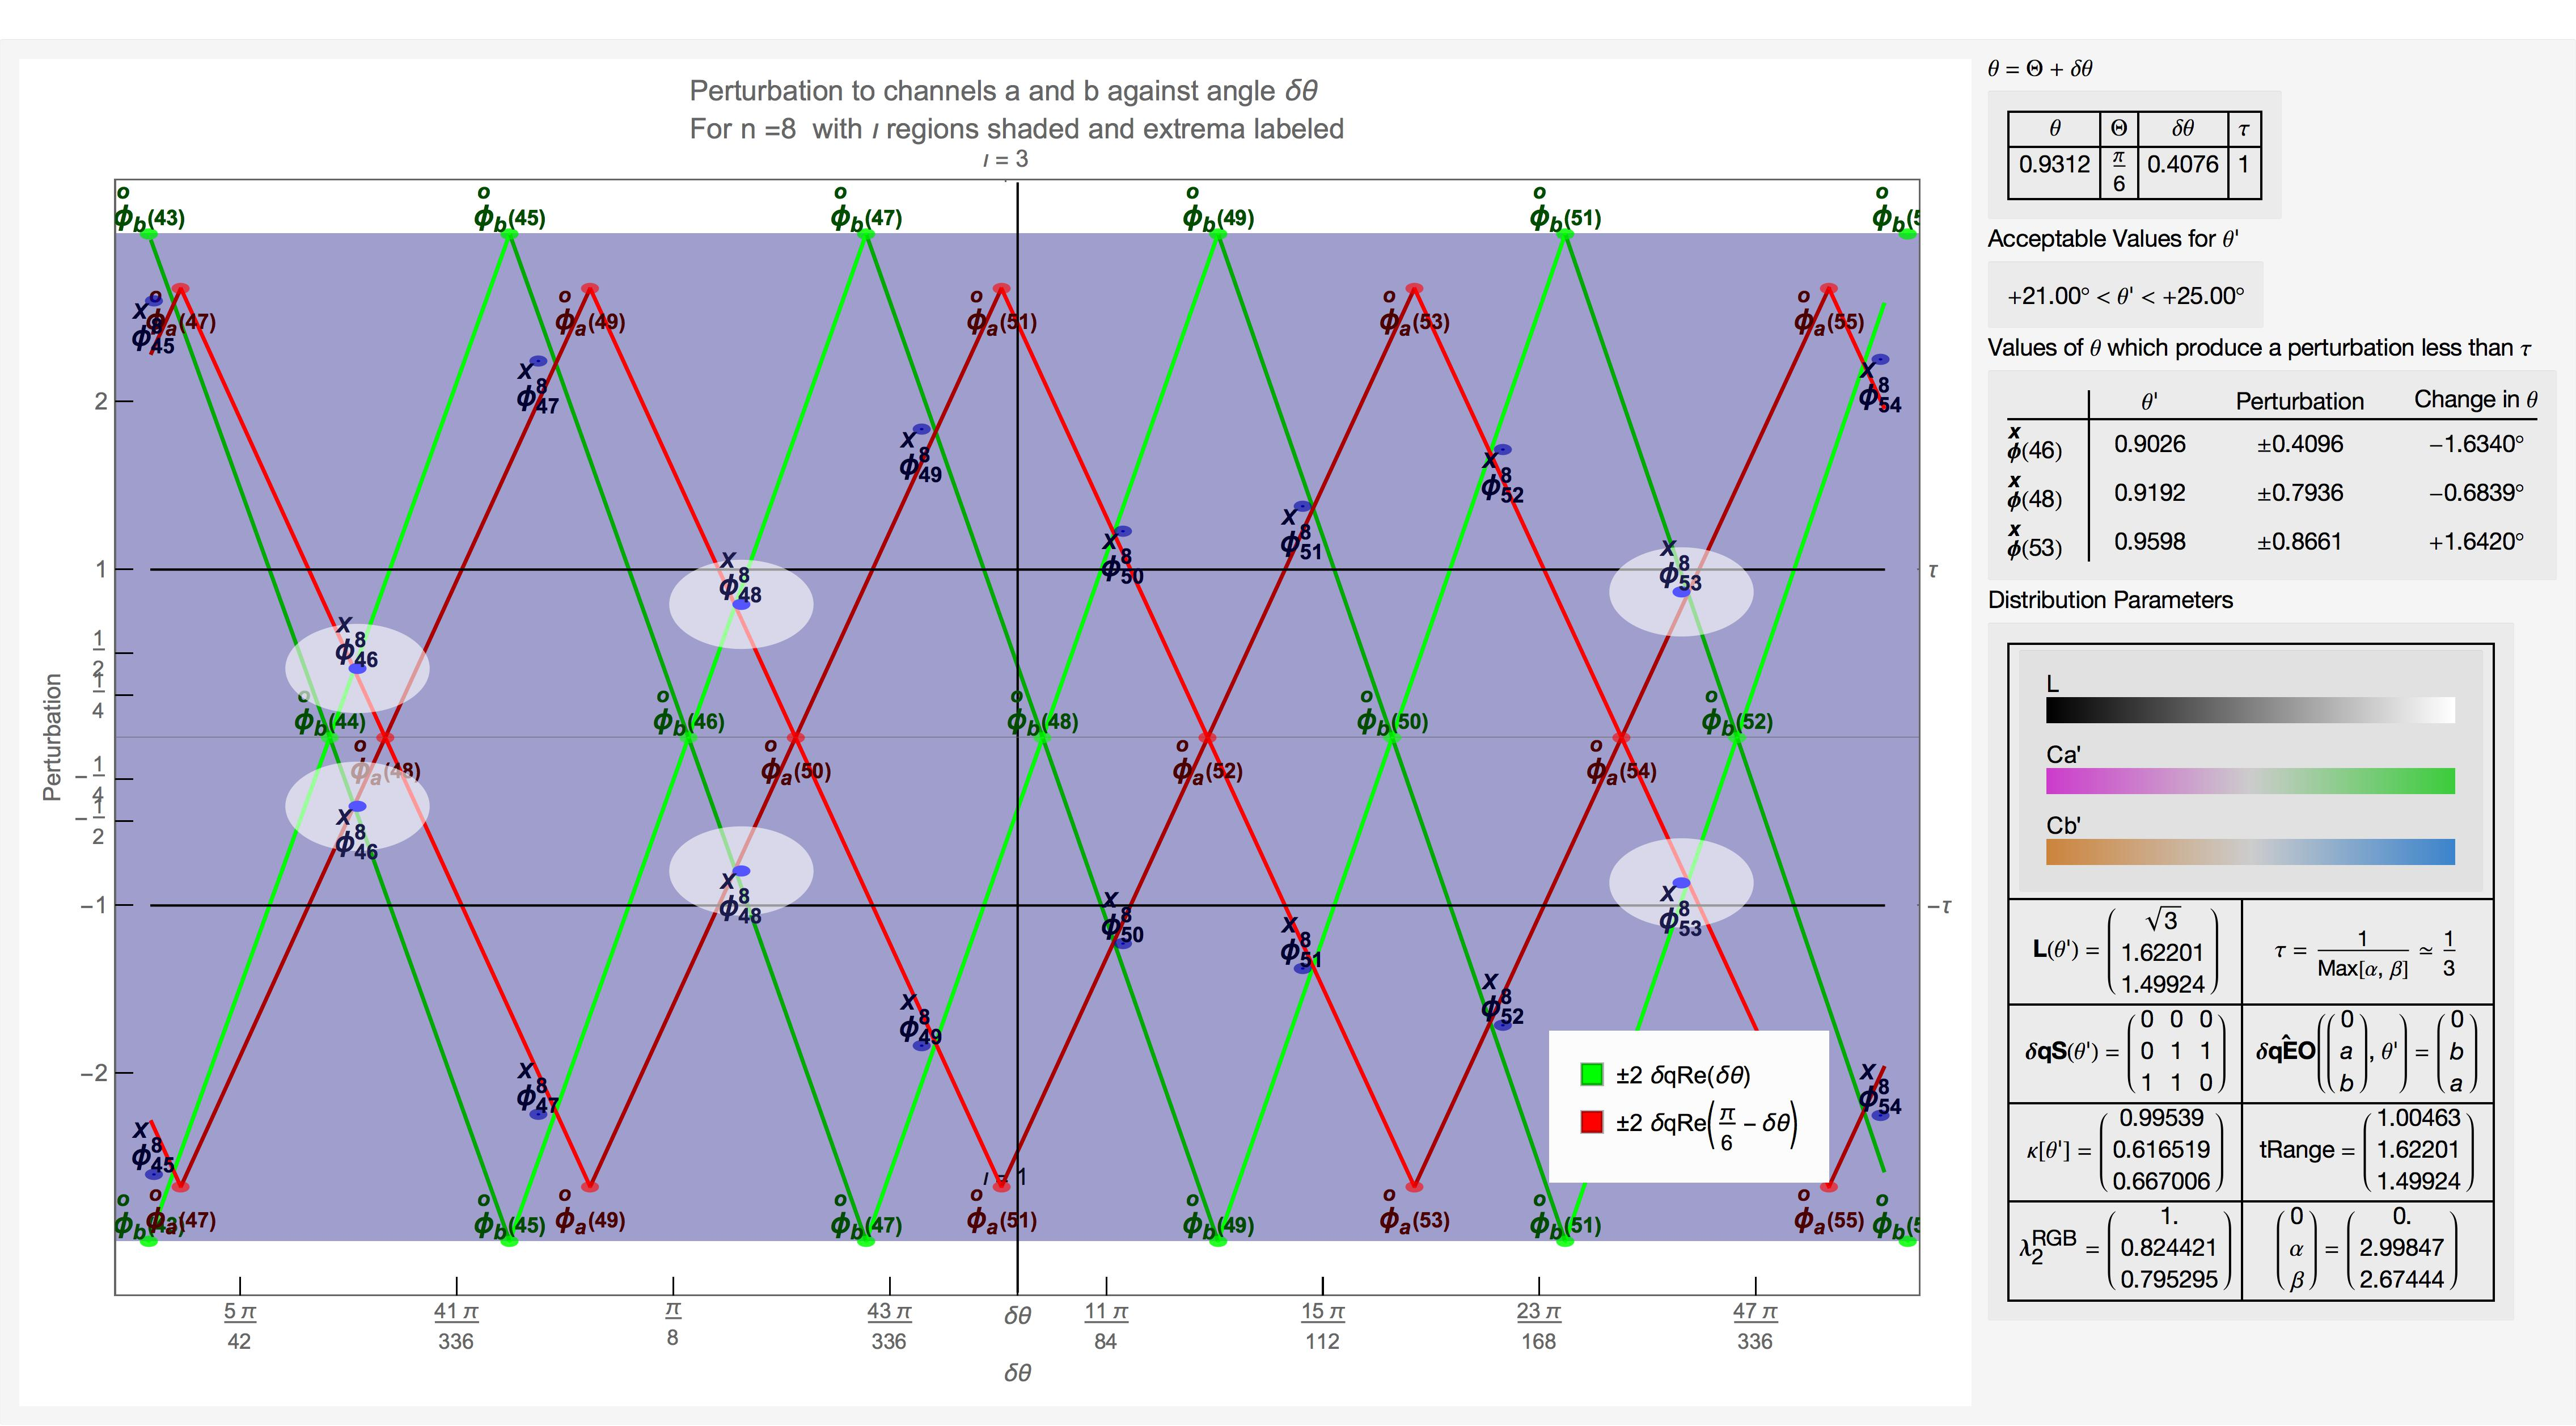
\includegraphics[width=1.0 \textwidth]{Chapter3/Figs/Channel_Perturbations_Angle_Decision_AB.jpg} 
    \caption{The channel perturbations within $\frac{\pi}{84}$ of $\theta'$. The channel perturbations are scaled by $\alpha$ and $\beta$ so a tolerance $\tau=1$ is used. Three angles satisfy the requirements}  \label{fig:PerturbationNearThetaAB}
\end{figure}

\begin{figure}[h!]
  \centering
  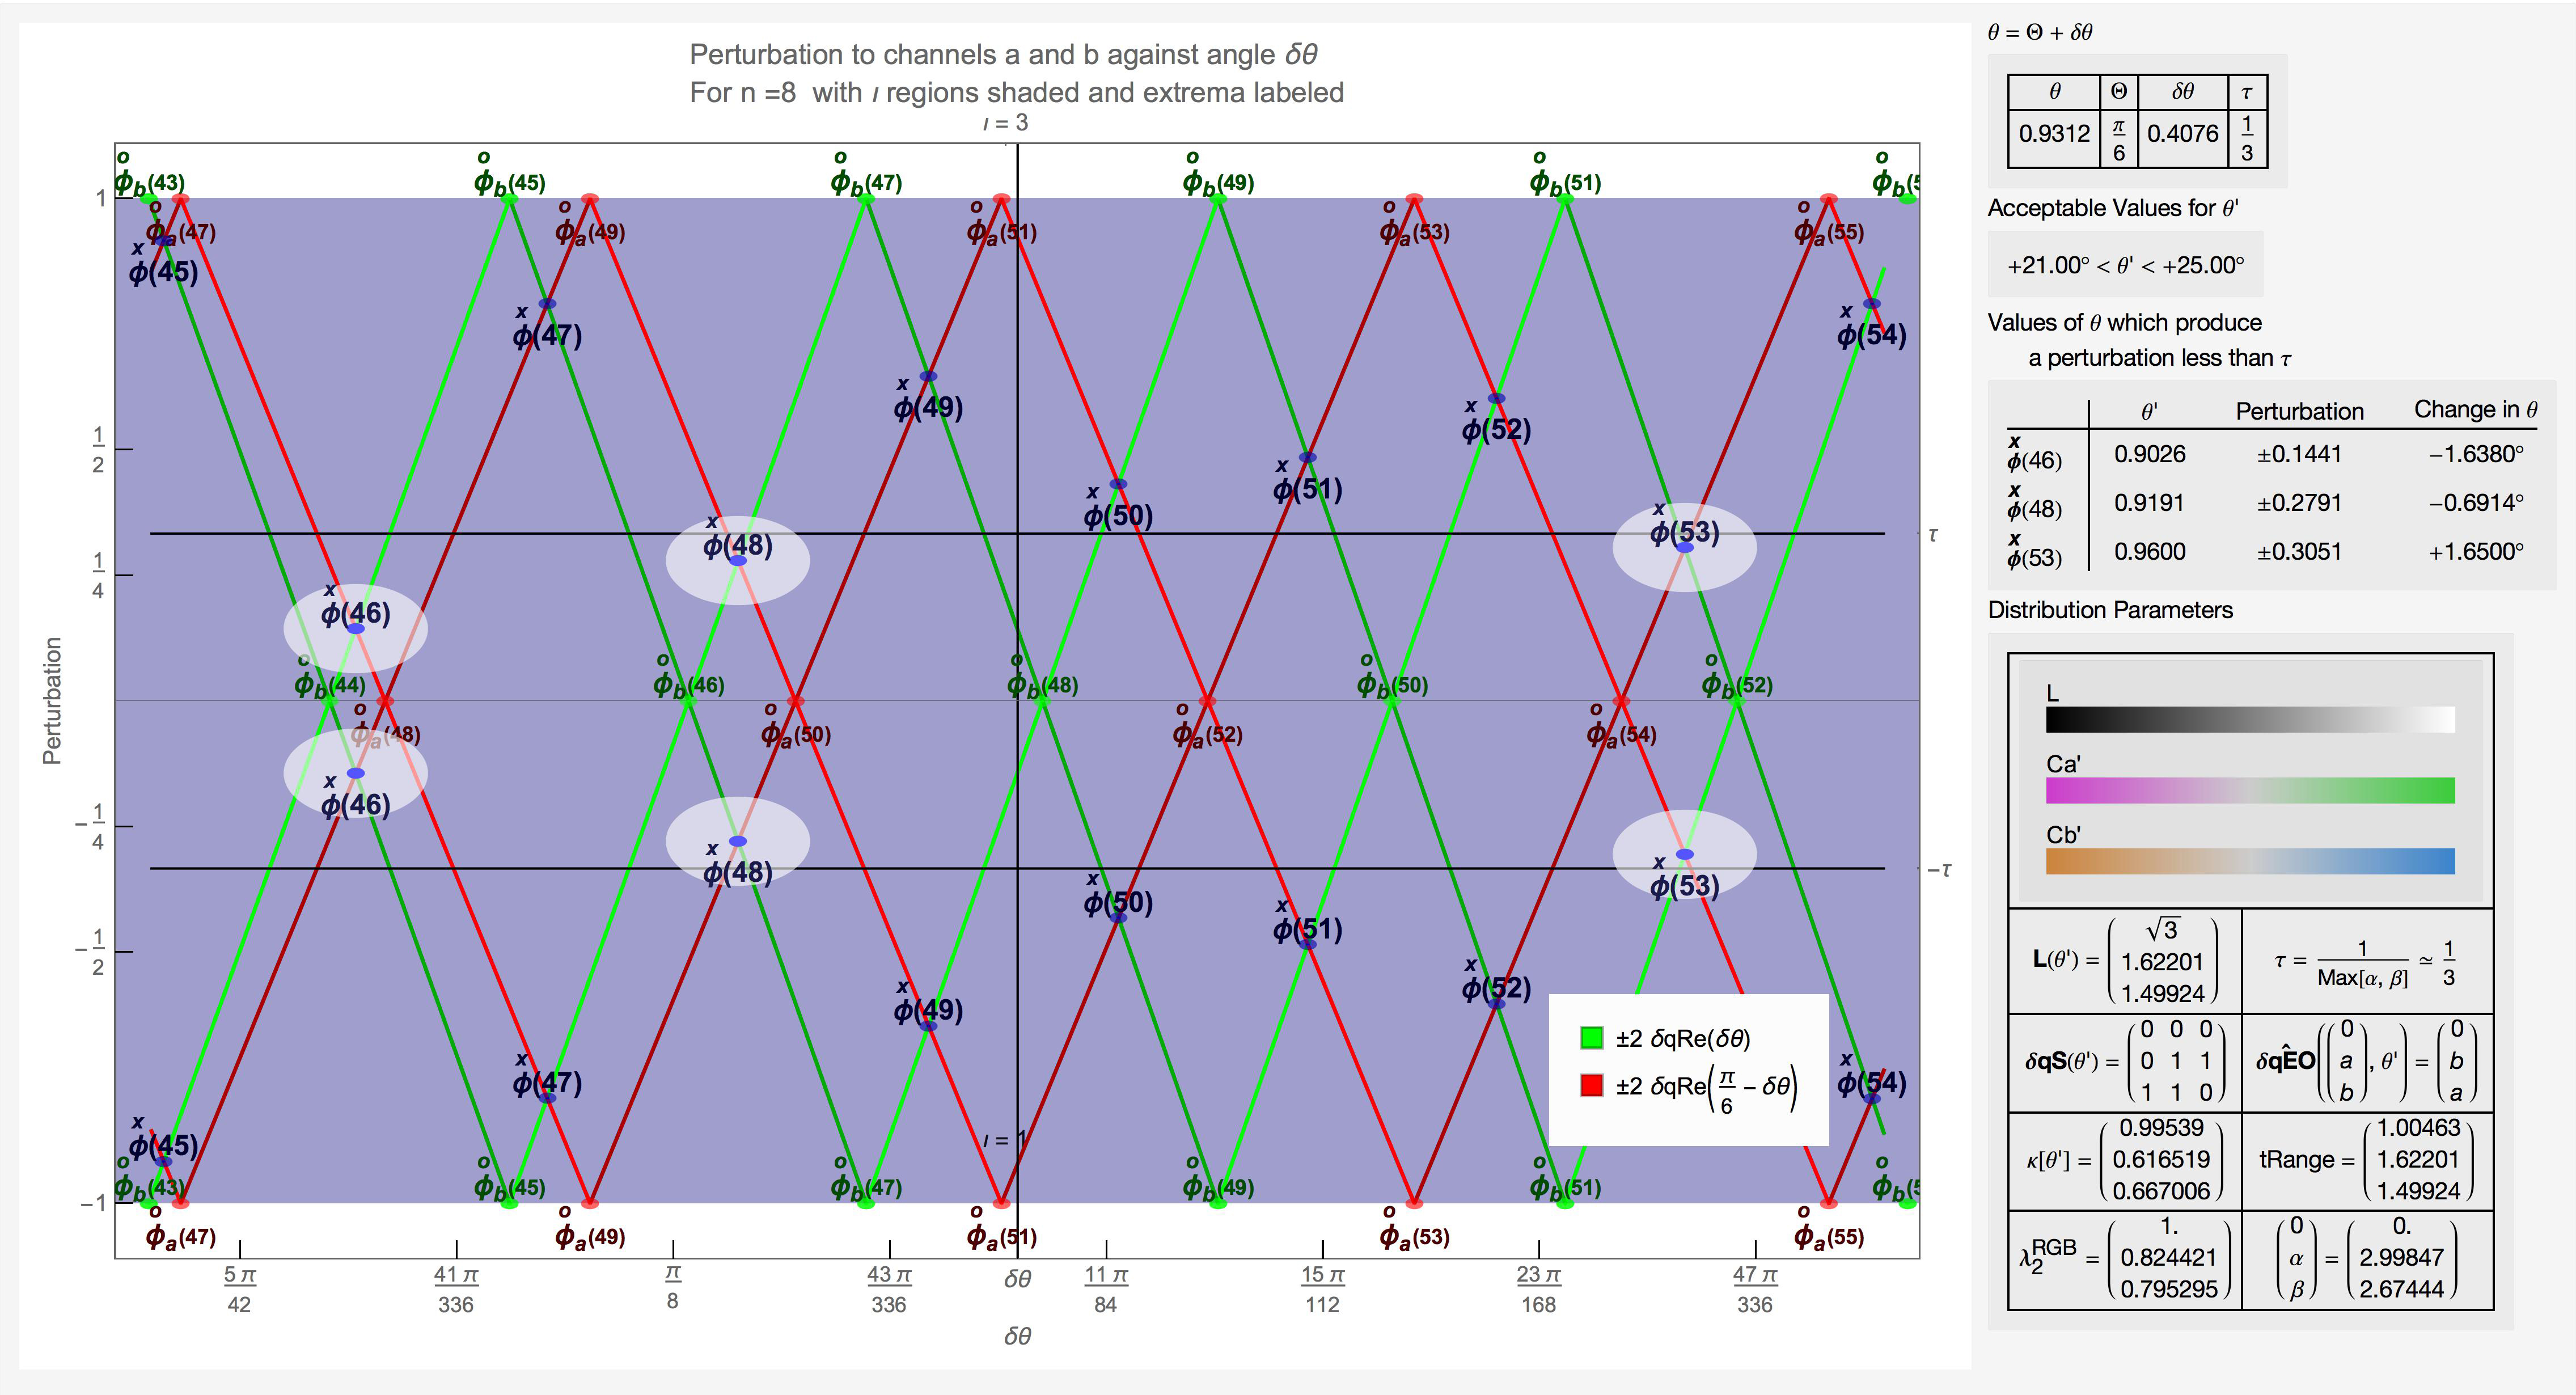
\includegraphics[width=1.0 \textwidth]{Chapter3/Figs/Channel_Perturbations_Angle_Decision_T.jpg} 
    \caption{The channel perturbations within $\frac{\pi}{84}$ of $\theta'$.}  \label{fig:PerturbationNearThetaT}
\end{figure}

We now follow the procedure outlined in chapter 2 and obtain an angle informed by computational considerations.  
With the perturbations to each channel scaled by their relative importance (Figure \ref{fig:PerturbationNearThetaAB}) there are three angles which satisfy the criteria.
 The algorithm returns the closest angle to the requested angle which is $\overset{x}{\phi } (48)$ however the perturbation is close to the tolerance of 1 which suggests that if the distribution parameters were adjusted to fit a particular individual then the perturbation may slip above the tolerance. 
 The channel scaling $\left\{ \alpha, \beta\right\} $ are also fairly close in value so the unscaled perturbations can be used with a tolerance $\tau = \text{Max}\left(\alpha, \beta\right)$ Figure \ref{fig:PerturbationNearThetaT}. 
 Accounting for both low perturbation and future adaptability a final angle $\theta = \overset{x}{\phi }(46) = 0.9025768293268257$ was chosen.

\begin{figure}[h!]
  \centering
  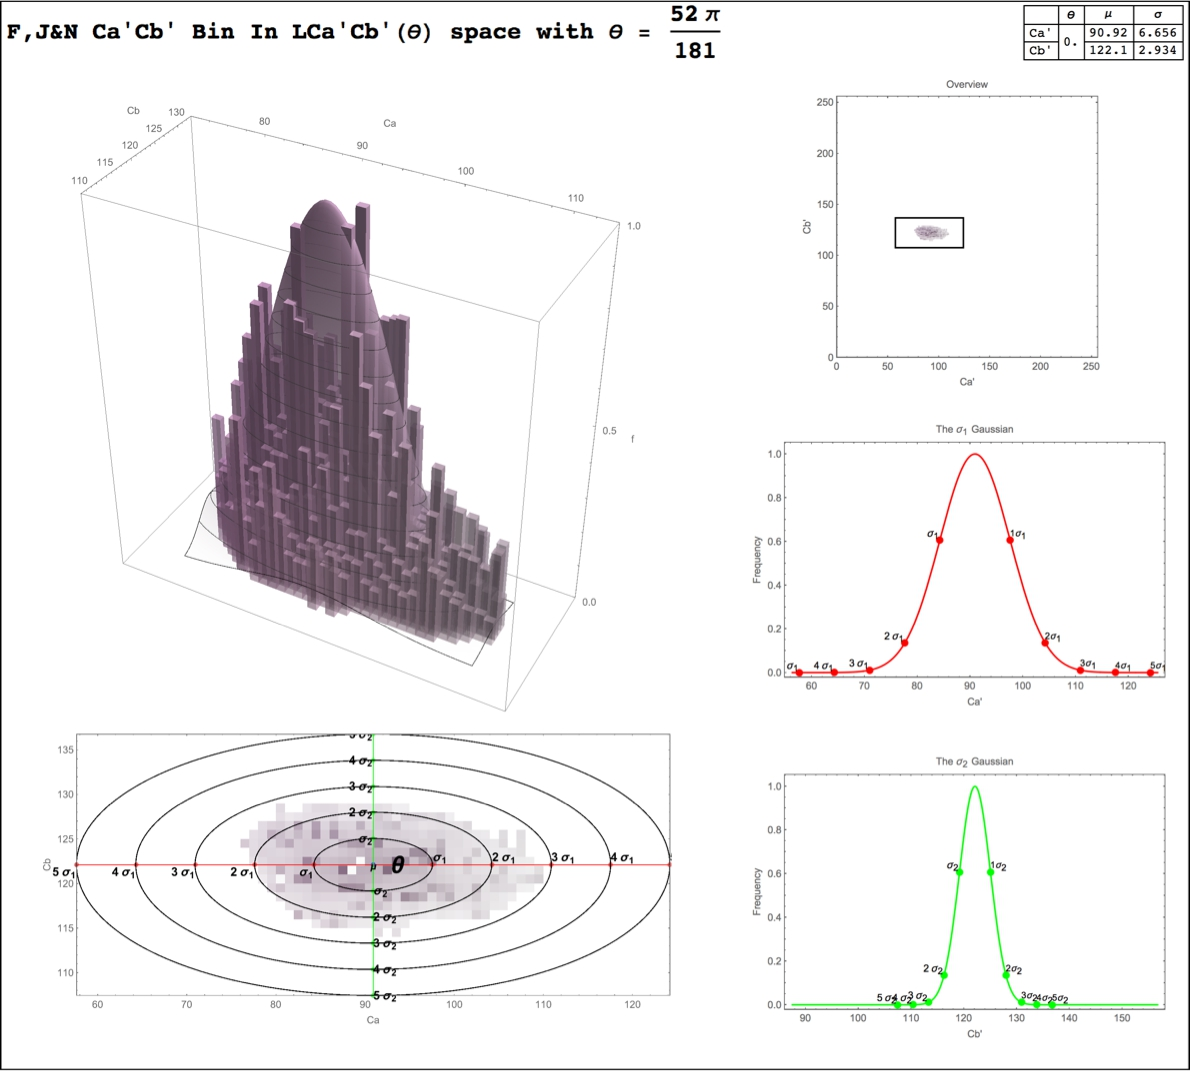
\includegraphics[width=1.0 \textwidth]{Chapter3/Figs/Fit_the_Gaussian_Final.jpg} 
    \caption{The Product of Gaussians fit to the three individuals statistics in the LCa'Cb' color-space.  }  \label{fig:FittheGaussianFinal}
\end{figure}

\begin{figure}[h!]
  \centering
  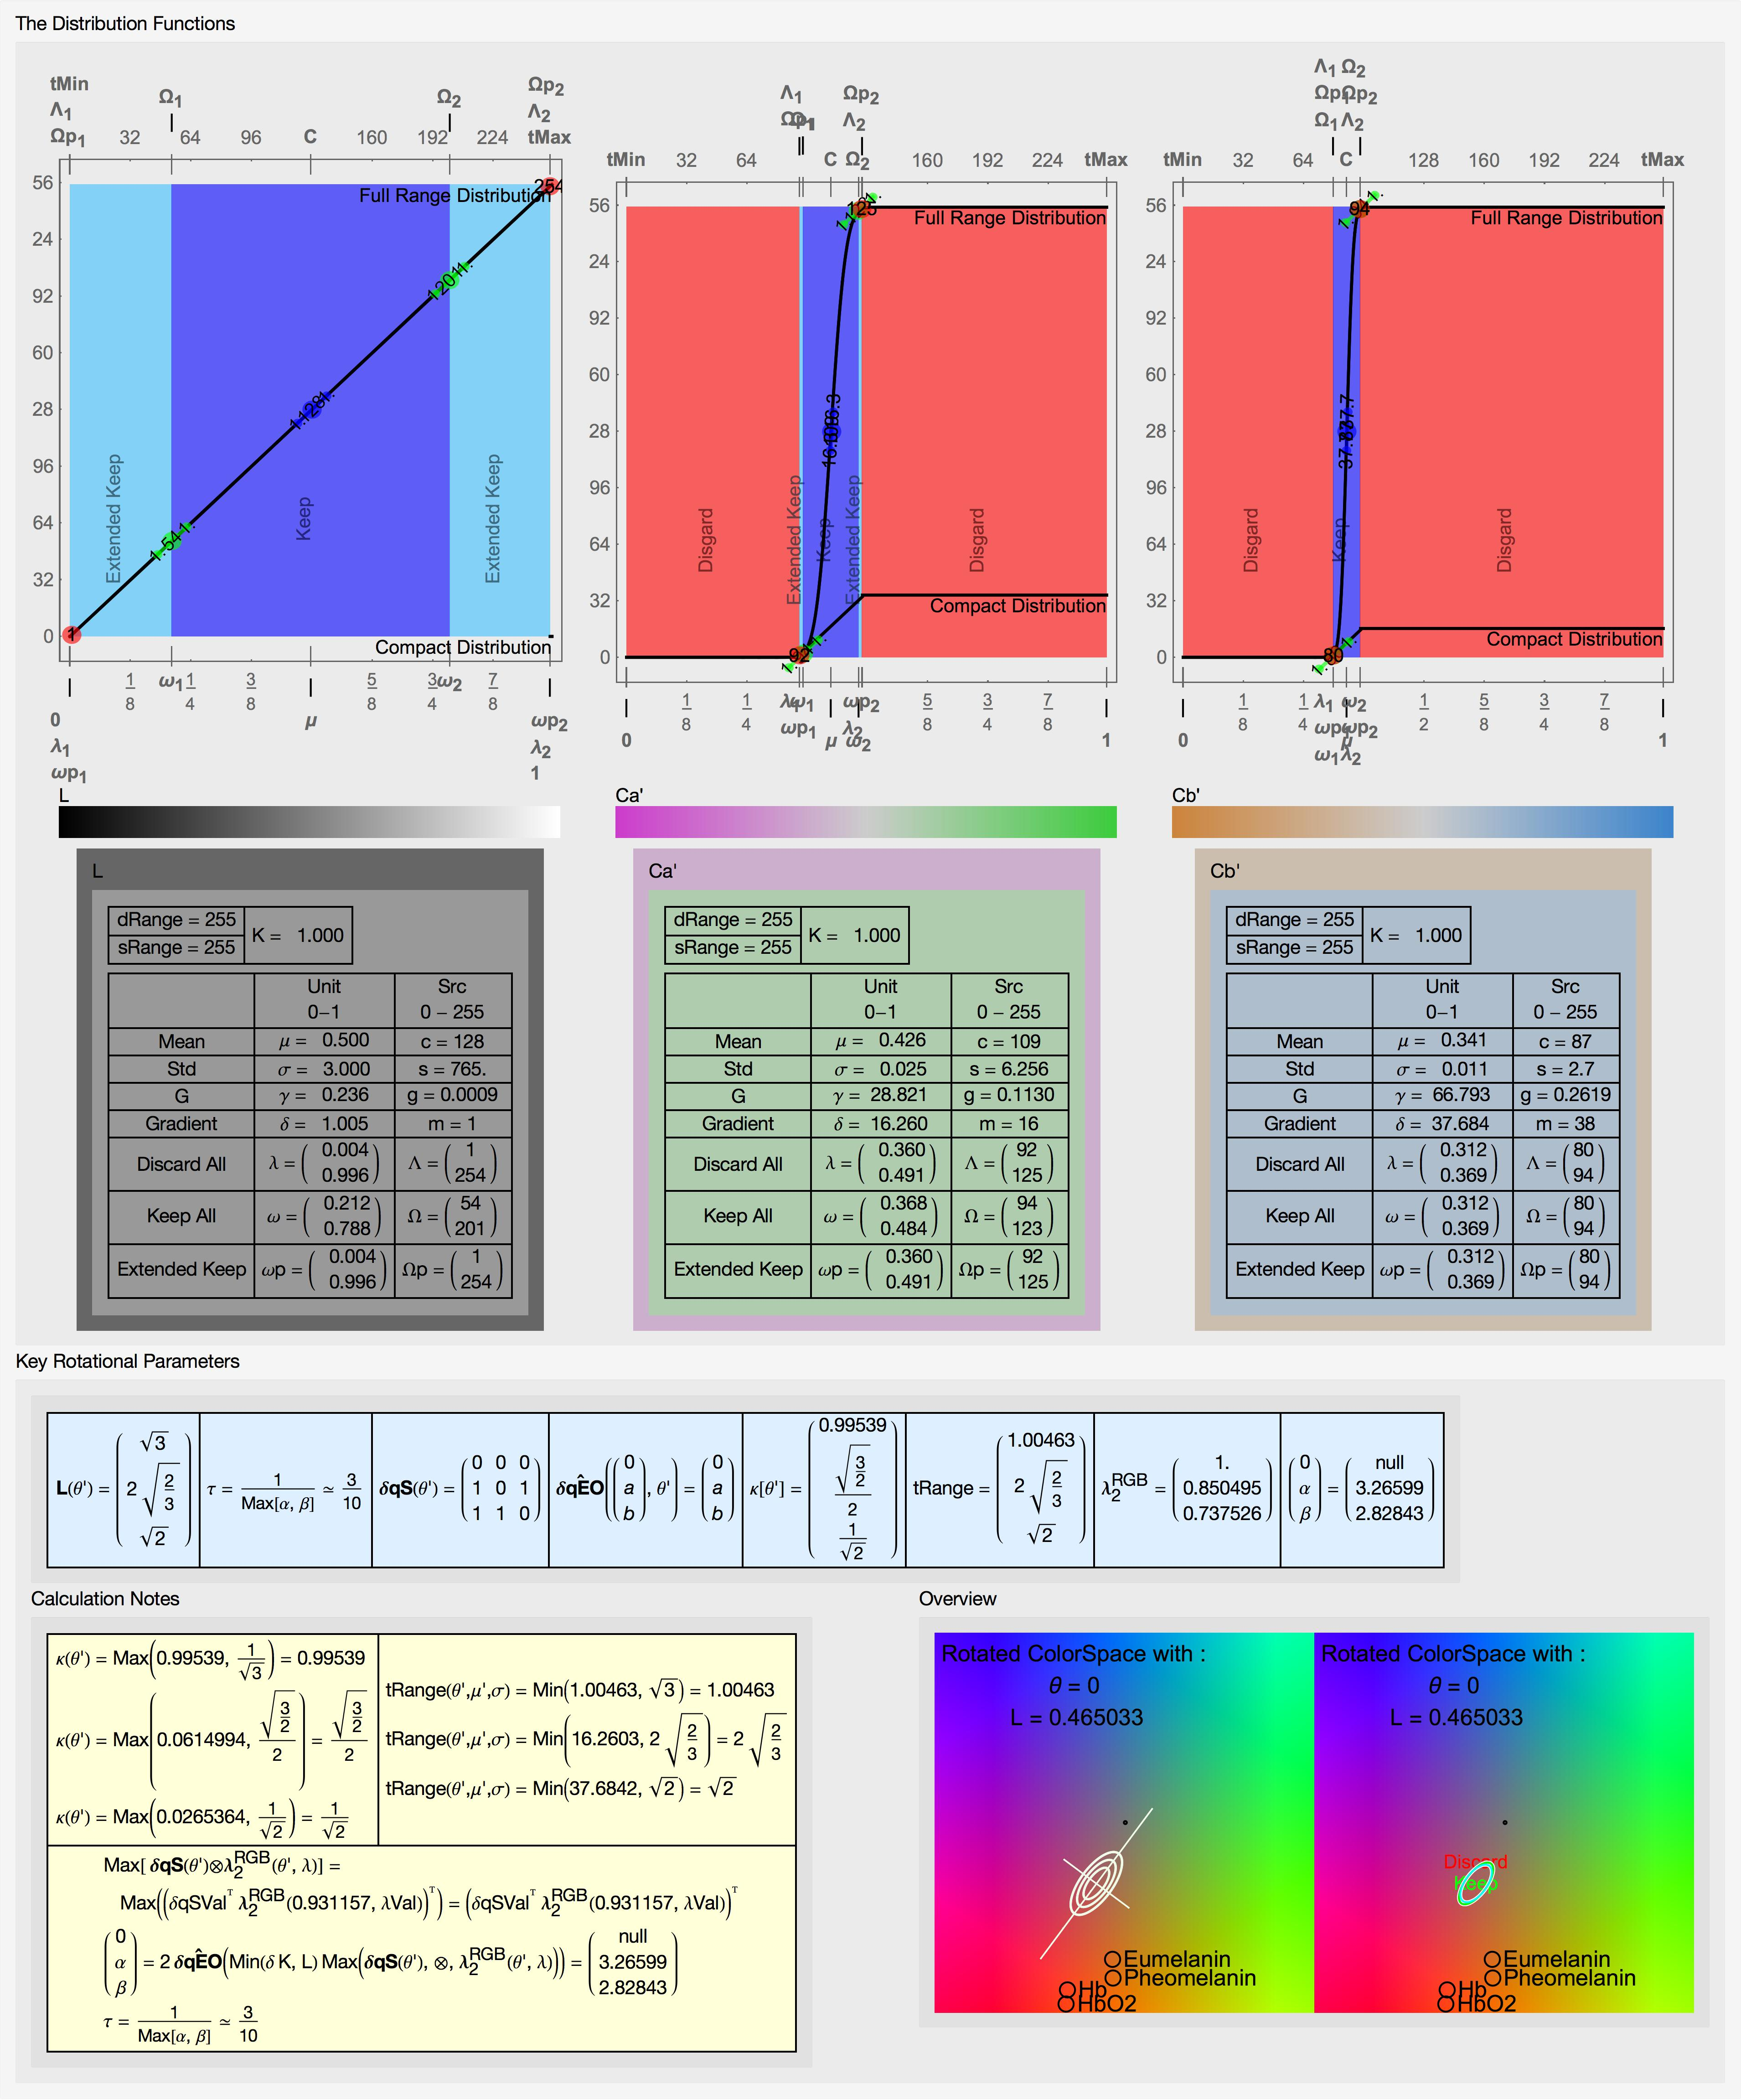
\includegraphics[width=1.0 \textwidth]{Chapter3/Figs/Distribution_Results.jpg} 
    \caption{ The redistribution functions for each axis alongside summary tables of the key parameters and a selection of calculations and an overview of the distribution in the new color-space  }  \label{fig:DistributionResults}
\end{figure}

As a final step, the MATLAB statistics gathering routine was run again using the combined F,J\&N RGB bins as a starting point and then rotating to the LCa'Cb' color-space with the new value for $\theta$. This was done partly to check that the code works as expected and to see how well the product of Gaussians function fits the distribution. The only difference to the MATLAB code was that for this run the Gaussian fit was found using equation \ref{eq:2DGaussianProd} which is the product of two 1D Gaussians with a fixed amplitude of 1. The result can be seen in Figure \ref{fig:FittheGaussianFinal}. 

\begin{equation}\label{eq:2DGaussianProd}
\exp \left( -\frac{{\CaMu}^2}{2 \sigma_1^2} -  \frac{ { \CbMu }^2}{2 \sigma_2^2} \right) \quad \textbf{where} \quad \CaMu = \text{Ca}-\mu_1 \quad \text{and} \quad \CbMu = \text{Cb}-\mu_2 
\end{equation}



\begin{figure}[h!]
  \centering
  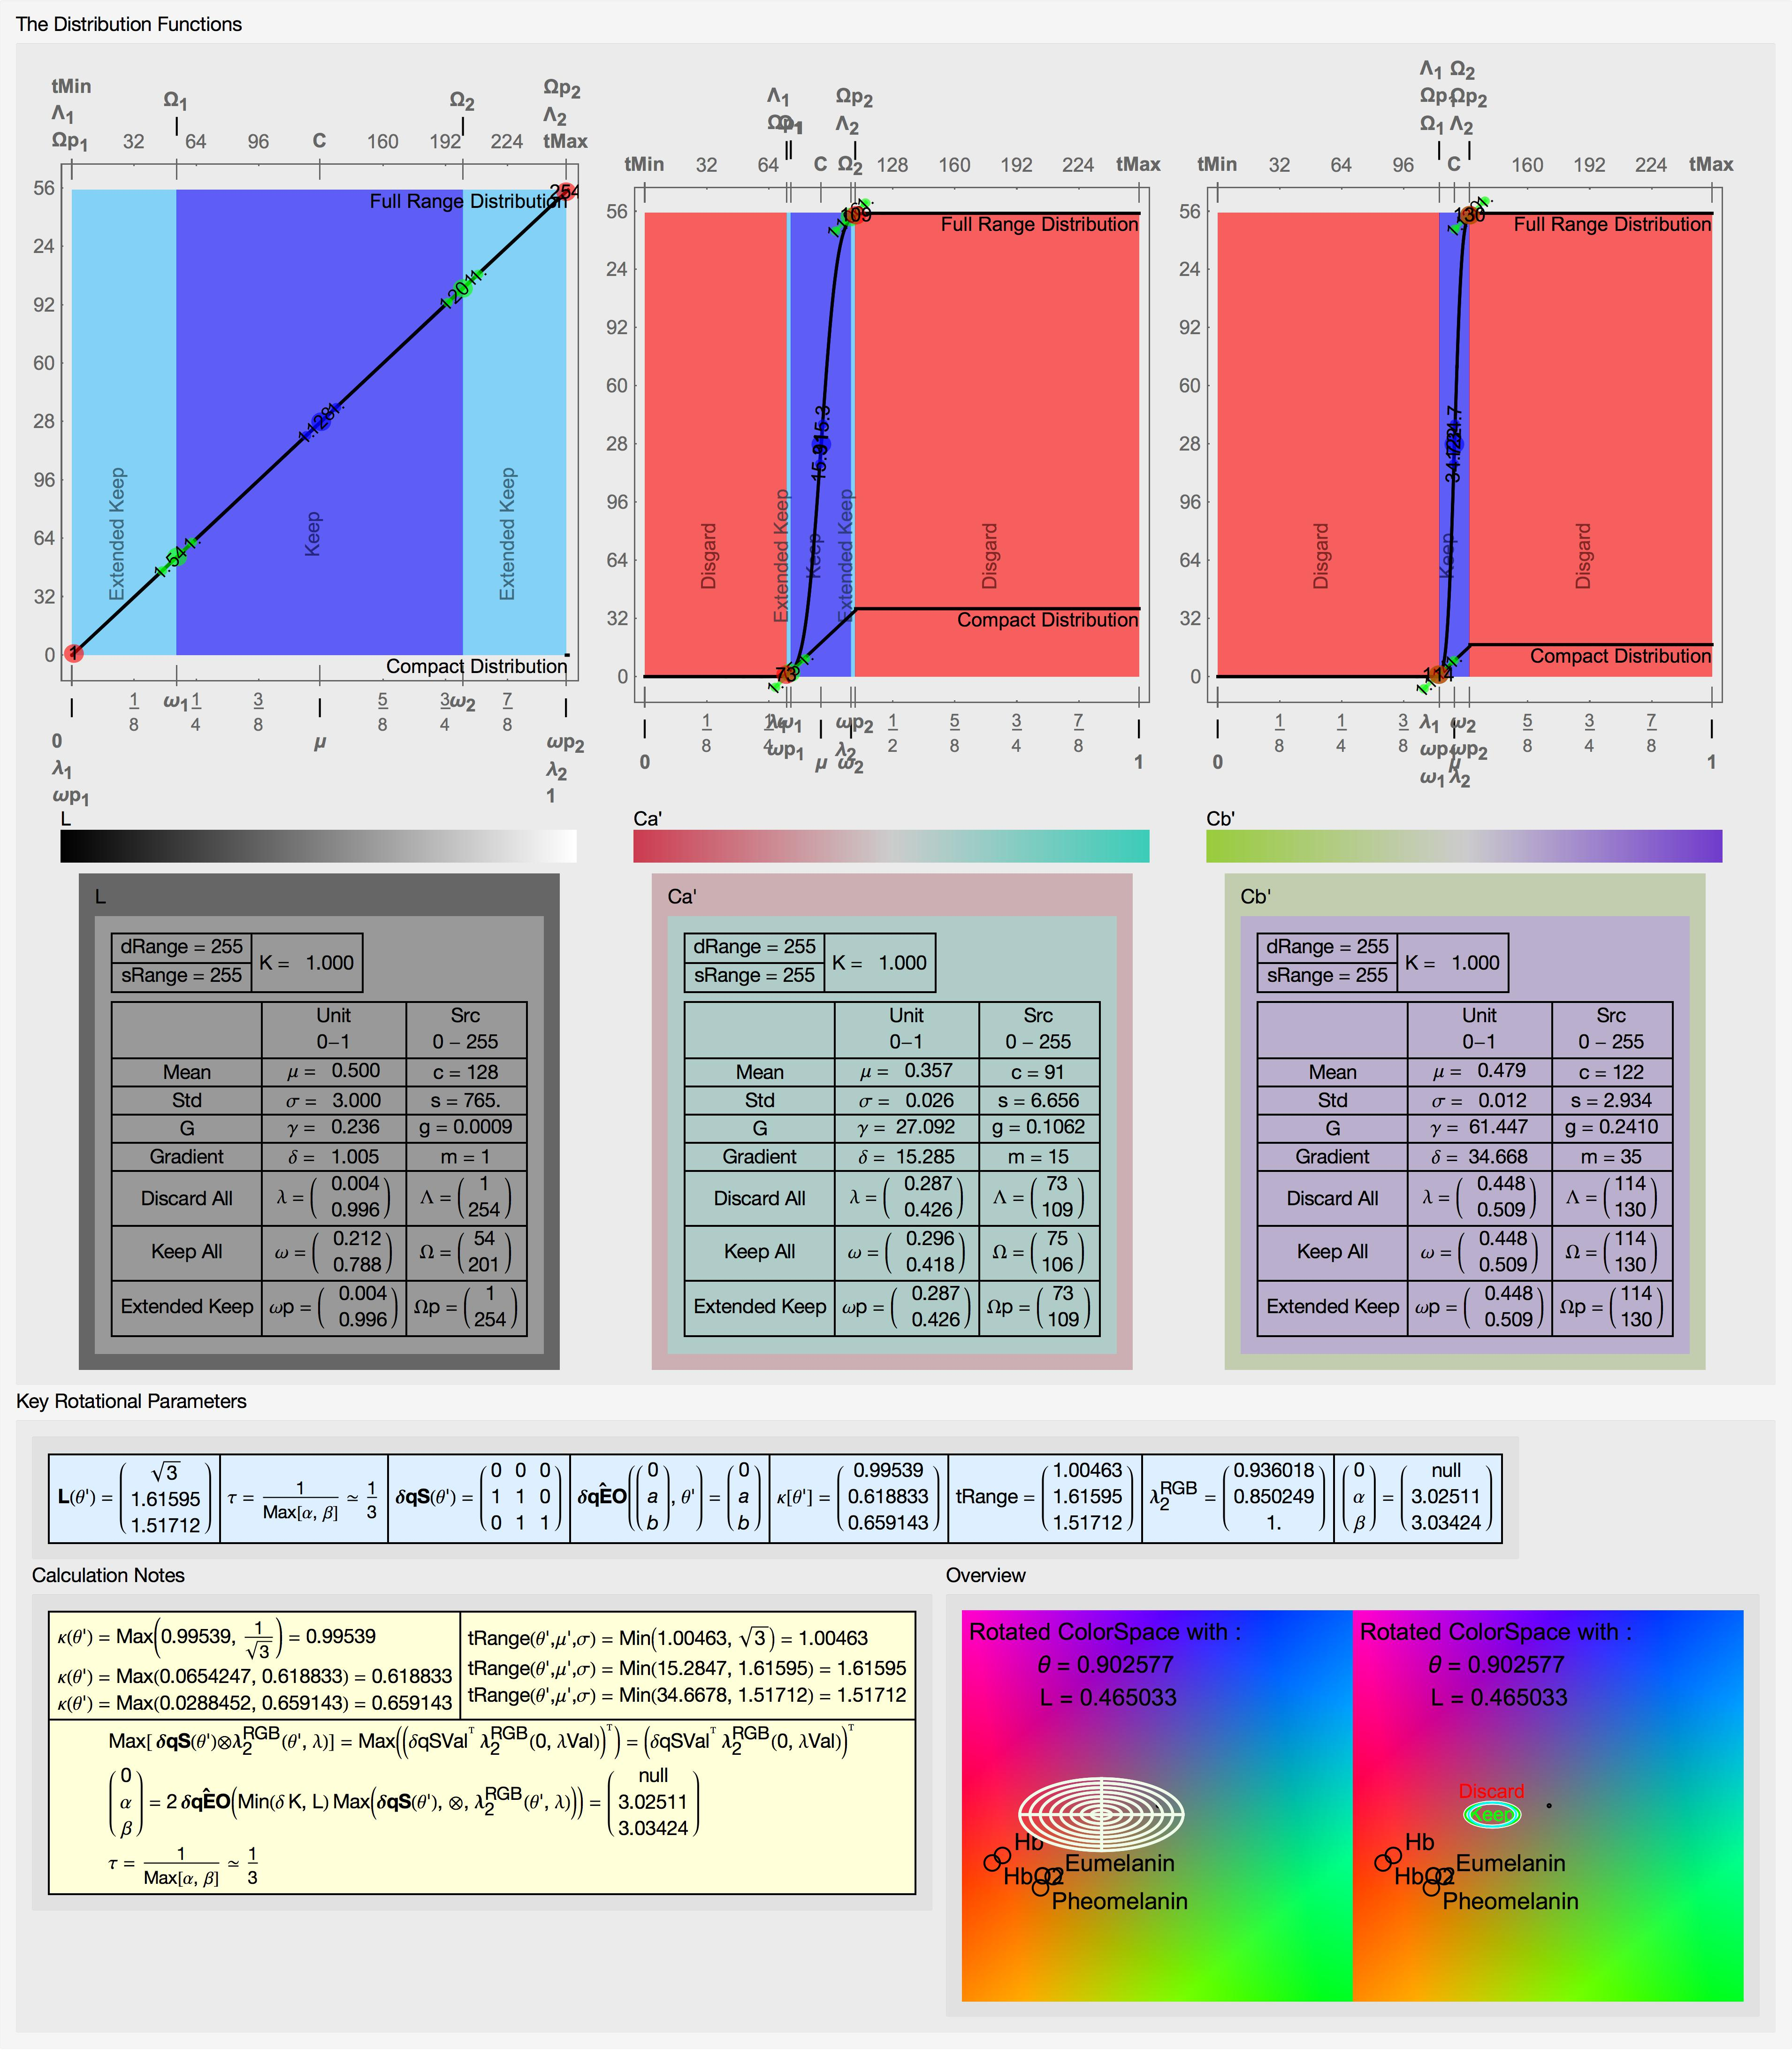
\includegraphics[width=1.0 \textwidth]{Chapter3/Figs/Distribution_Results_Final.jpg} 
    \caption{ \textbf{The Tight MATLAB fit in LCa'Cb'.} The redistribution functions for each axis alongside summary tables of the key parameters and a selection of calculations and an overview of the distribution in the new color-space.}  \label{fig:DistributionResultsFinal}
\end{figure}

It can be seen that the least square fit is a good predictor for the distribution but the aim of the color-space is to capture all skin relevant chromatic information. For this reason,  as well as the desire to be inclusive of skin tones outside of the sample set of three individuals, a region larger than the $2\sigma$ ellipse region (Figure \ref{fig:DistributionResultsFinal}) which is kept by the tight MATLAB fit may be desirable to be included. The $3\sigma$ ellipse region would include everything in the combined individual F,J\&N histogram. A $5\sigma$ ellipse region would  likely account for a wide variety of skin tones. 

\begin{figure}[h!]
  \centering
  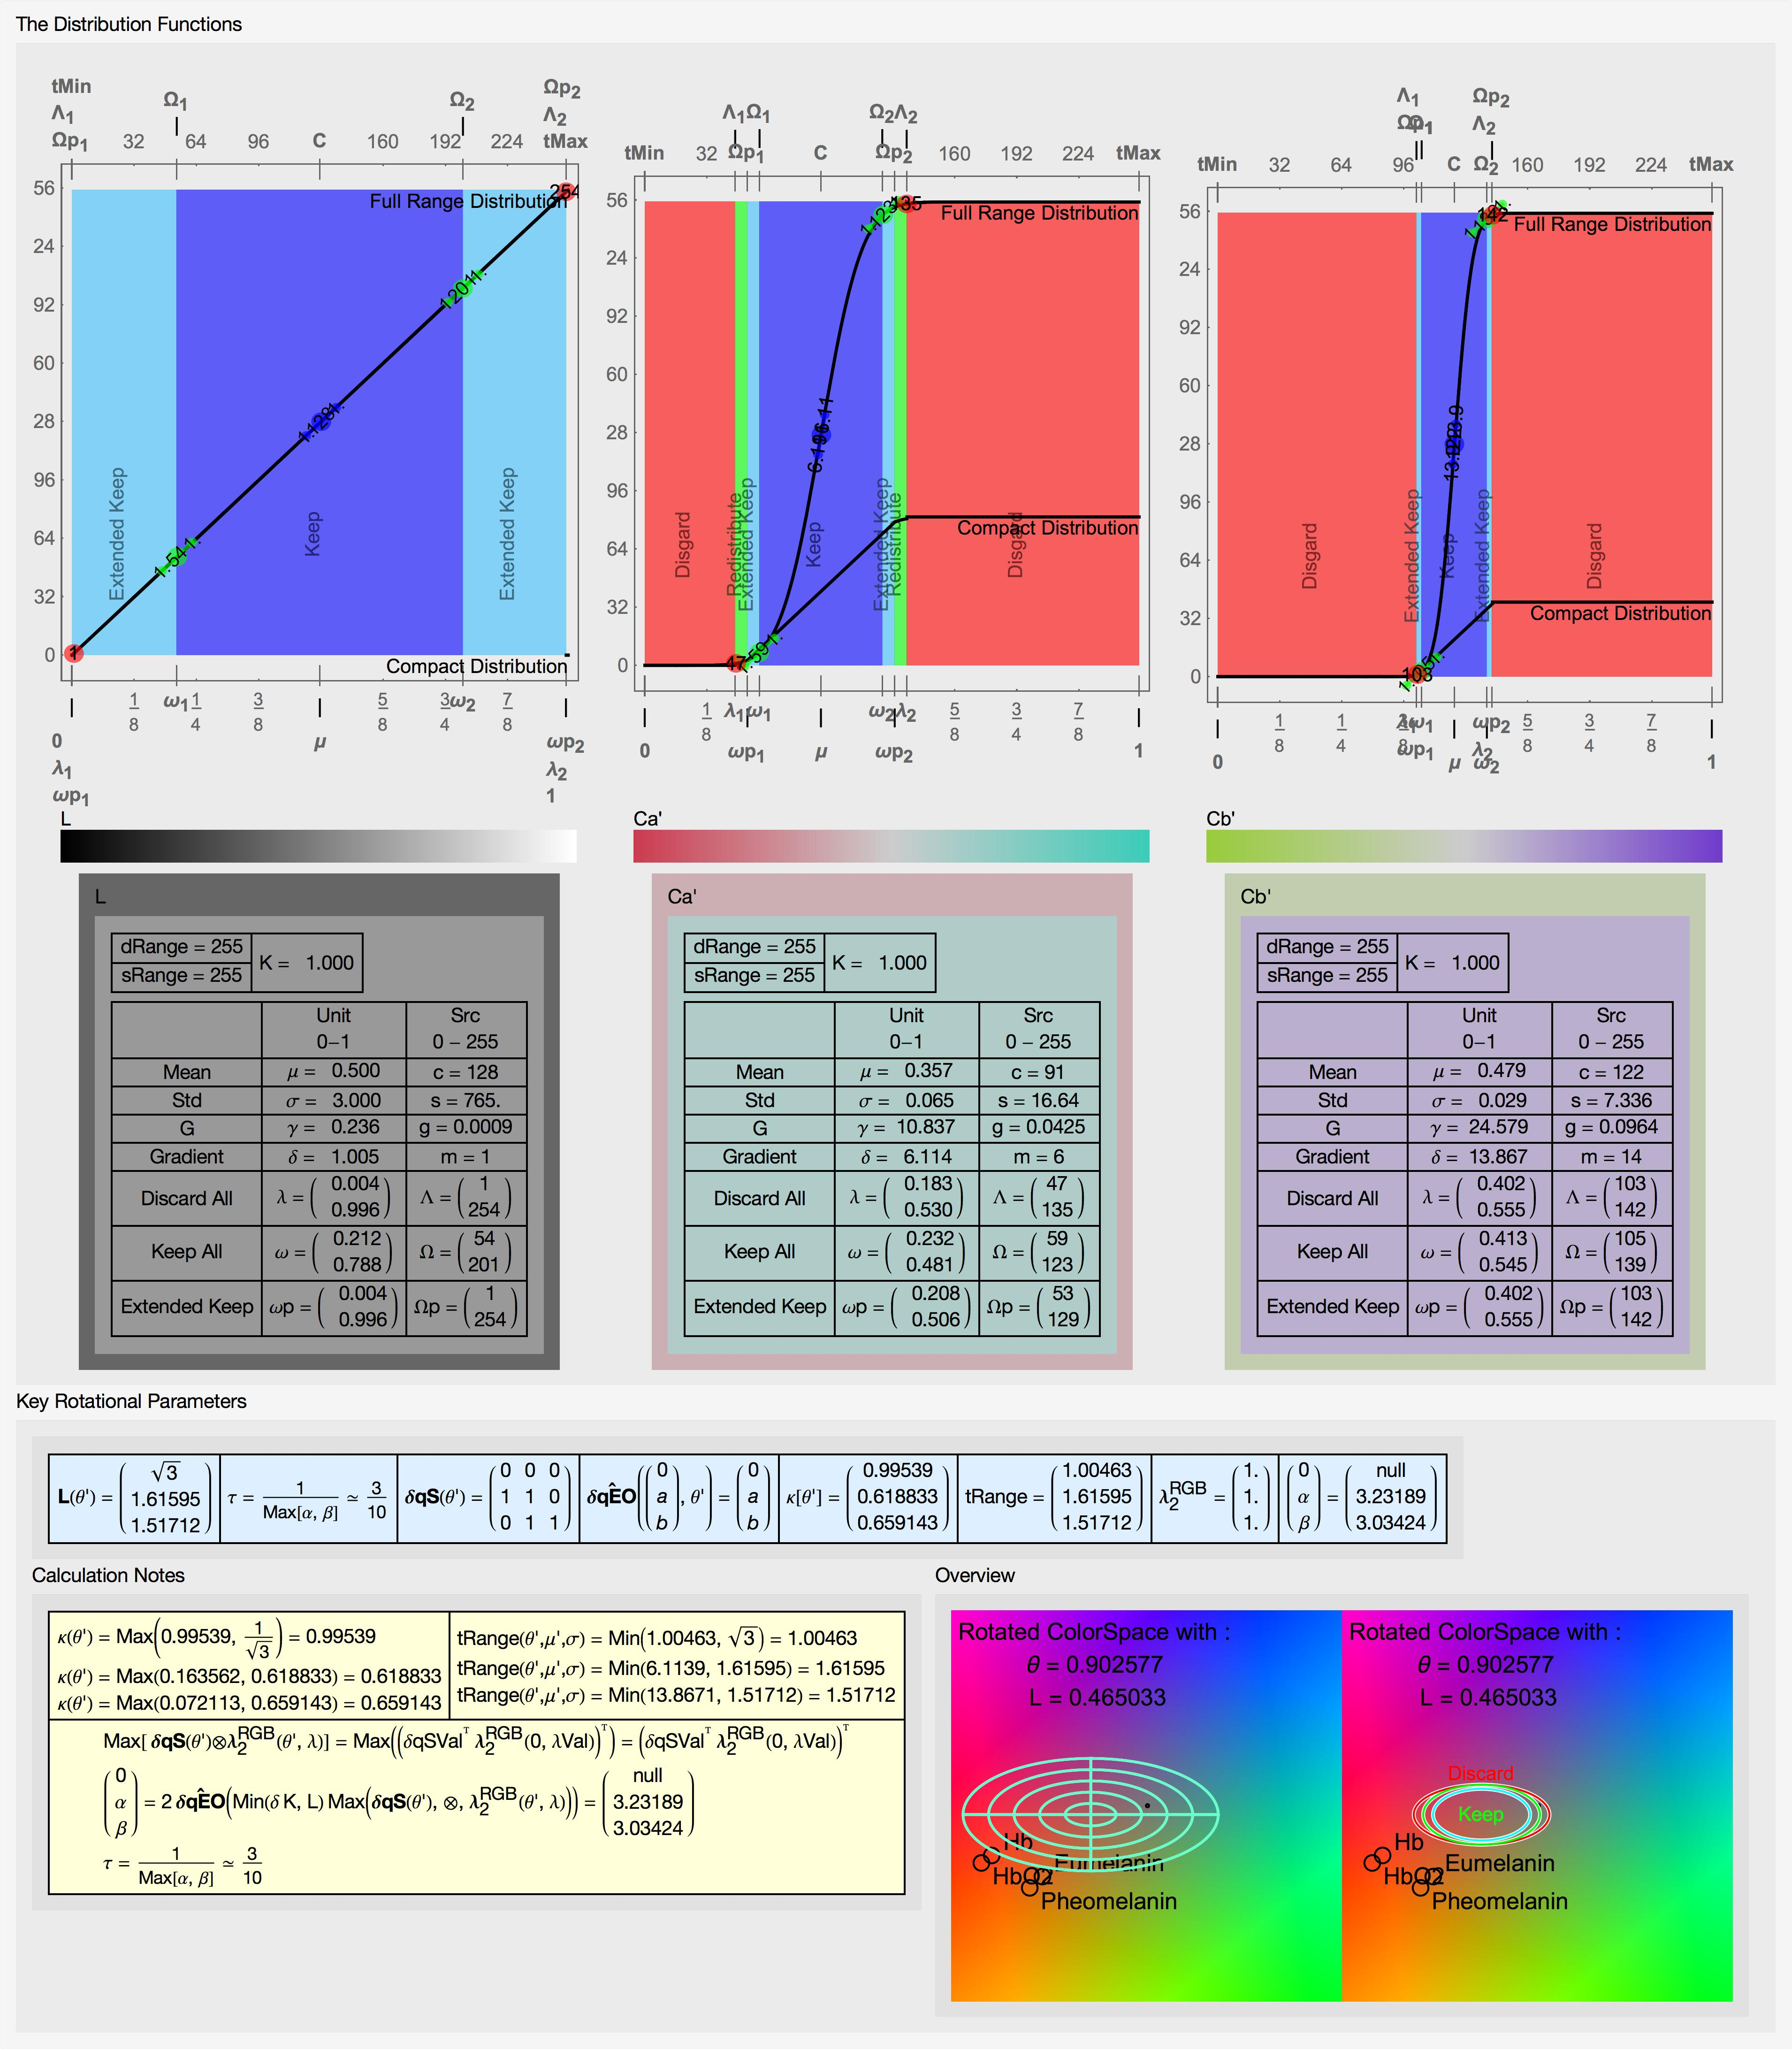
\includegraphics[width=1.0 \textwidth]{Chapter3/Figs/Distribution_Results_Final_Extended.jpg} 
    \caption{ \textbf{The extended $5\sigma$ ellipse region MATLAB fit in LCa'Cb'.} The redistribution functions for each axis alongside summary tables of the key parameters and a selection of calculations and an overview of the distribution in the new color-space. }  \label{fig:DistributionResultsFinalExtended}
\end{figure}

\begin{figure}[h!]
  \centering
  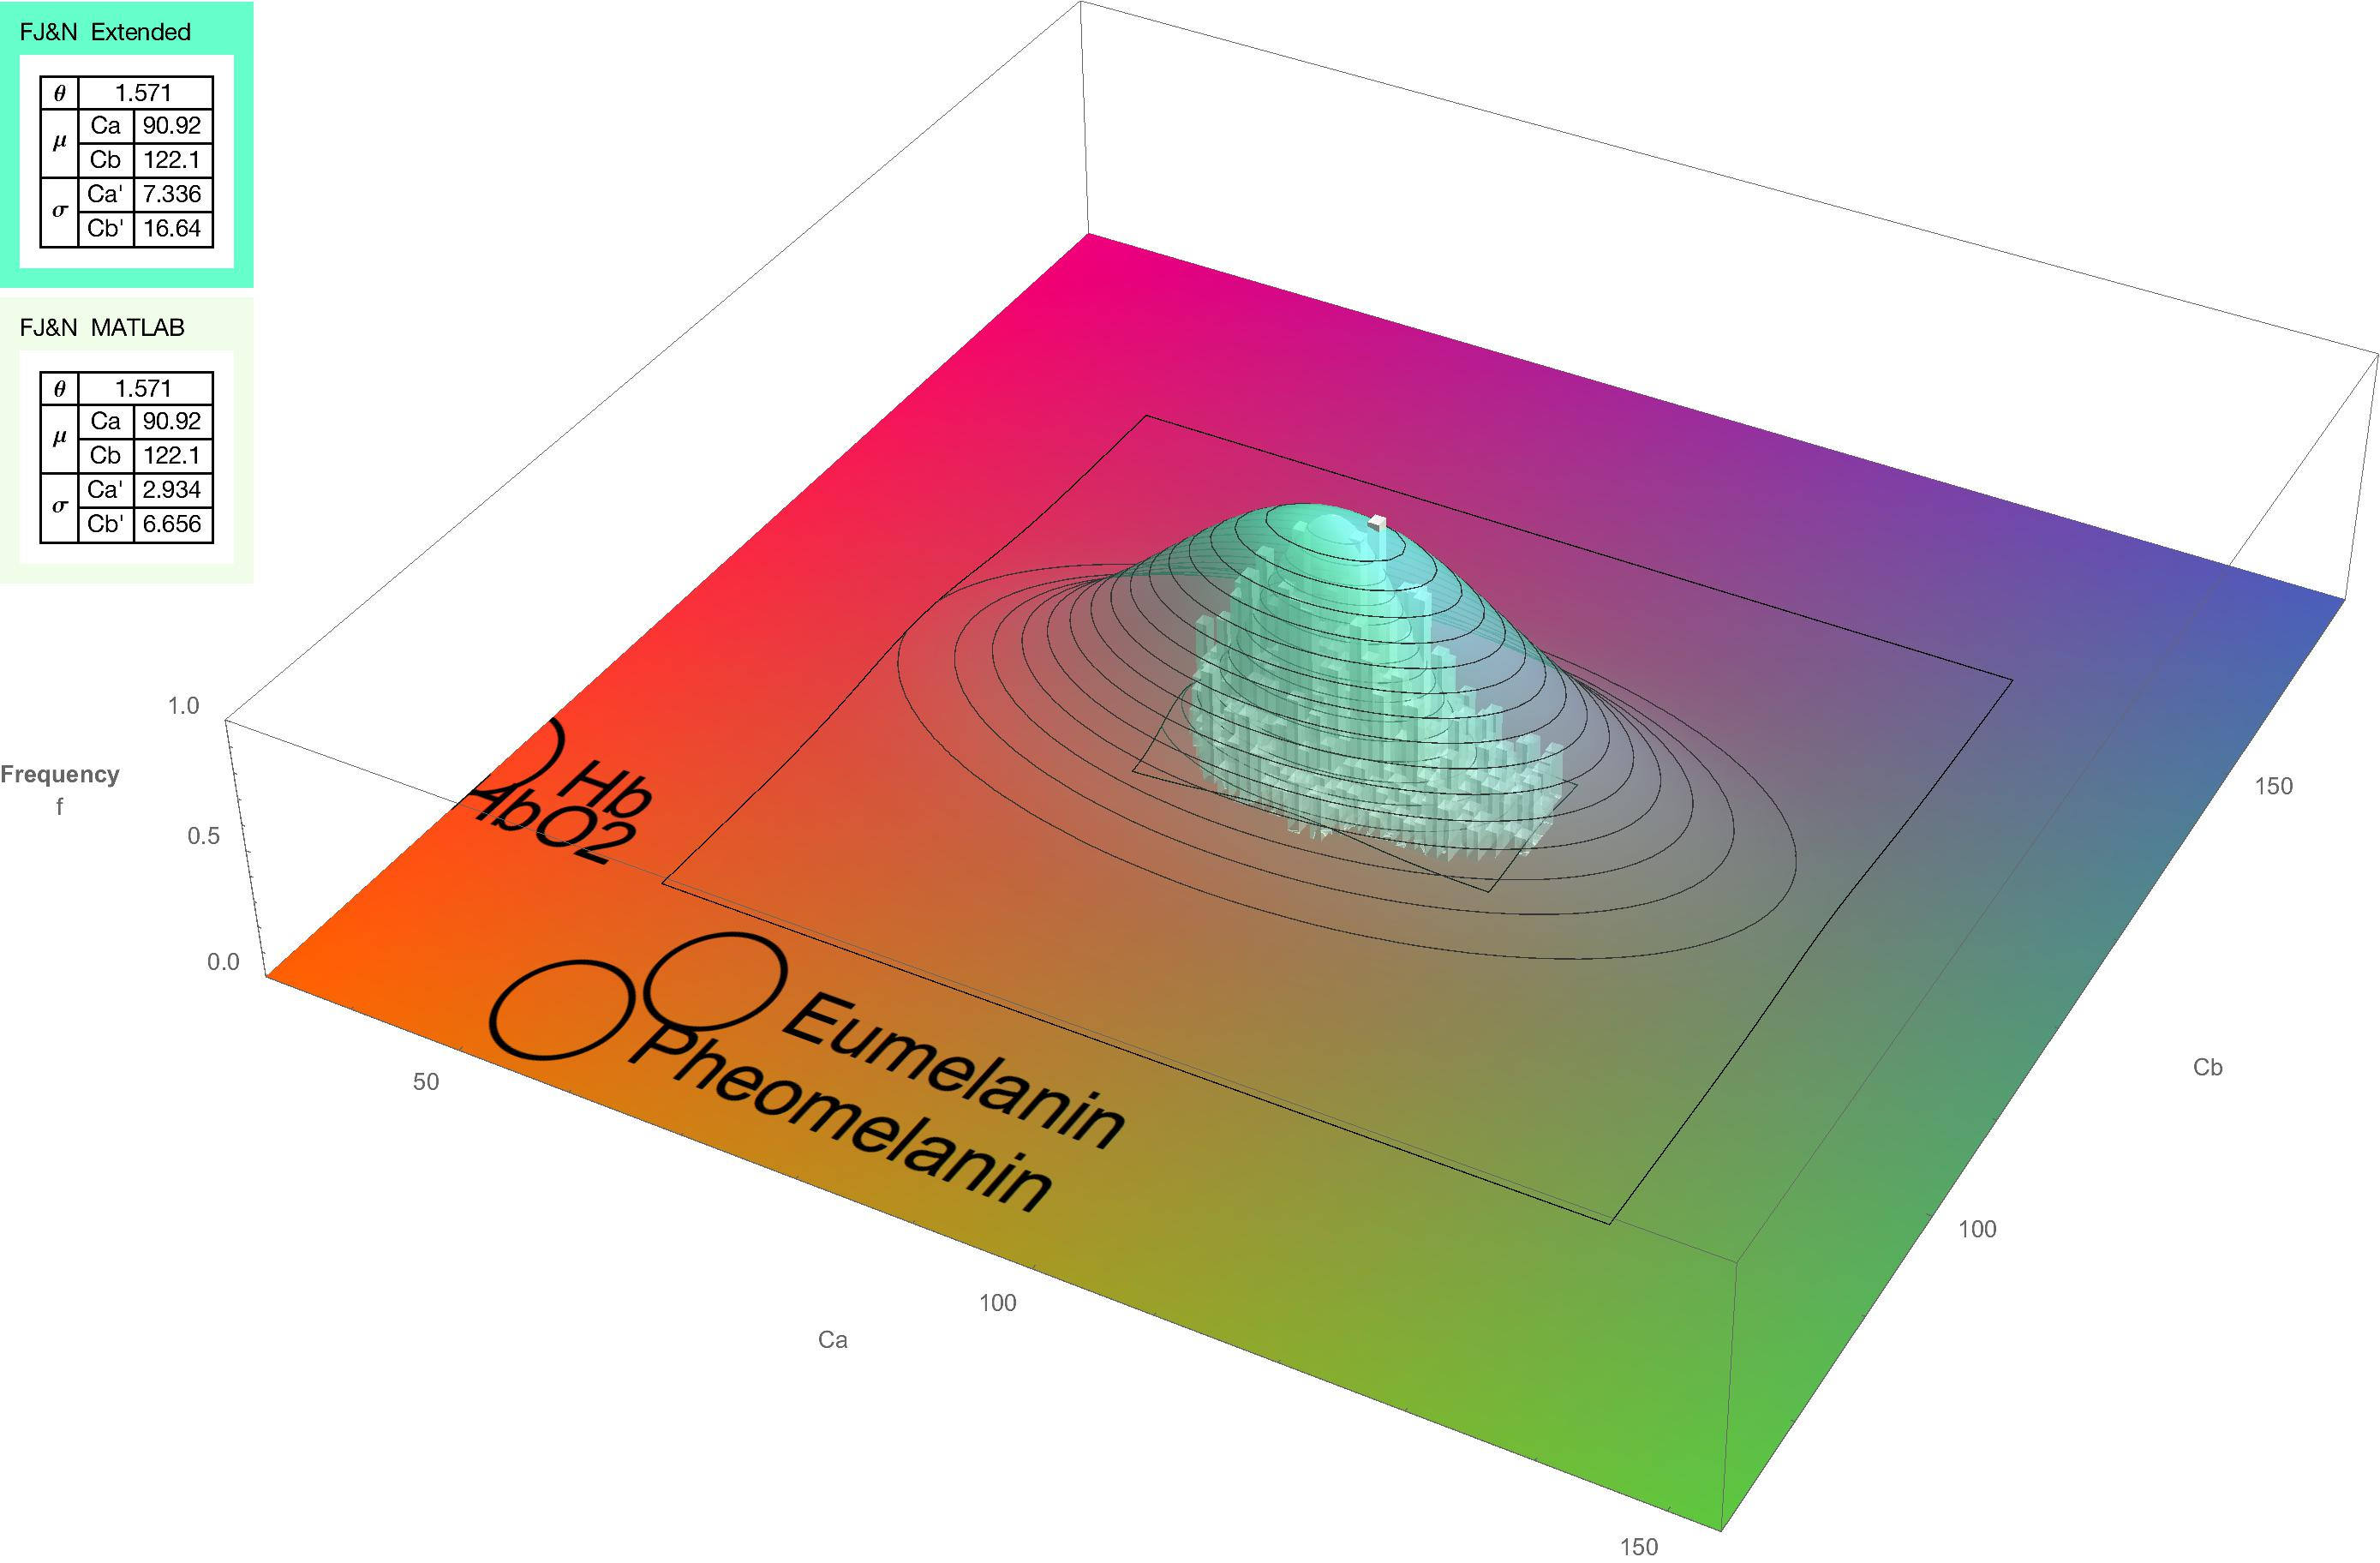
\includegraphics[width=0.95 \textwidth]{Chapter3/Figs/Distribution_Results_Final_Extended_3D.jpg} 
    \caption{ The tight and extended fits in the LCa'Cb' color-space.}  \label{fig:DistributionResultsFinalExtended3D}
\end{figure}

Extending the distribution may also affect the accuracy required in the rotation as mentioned previously. Extending out to a $5\sigma$ ellipse region does indeed affect the tolerance (Figure \ref{fig:DistributionResultsFinalExtended}), but the chosen angle perturbation $\pm0.144$ still satisfies the tolerance $\tau = 0.3094$ as $0.1441 < 0.3094$. It's also notable that the tight MATLAB distribution requires a partition in the chromatic axis while the extended distribution requires a small amount of redistribution. The tight MATLAB distribution and the extended distribution can be seen in Figure \ref{fig:DistributionResultsFinalExtended3D}.

\subsection{Conclusion}

Our goal was to find appropriate values for the 2D chromatic Gaussians in order to facilitate the image processing, and to create a color-space that preserves all of the chromatic skin information. To show that we have achieved this, we will quickly demonstrate the skin probability map:

After redistribution we have two new spaces in which to express the stats parameters: the 0-dstMax range and the new 0-1 range, where 0 and 1 correspond to different positions in the original unit space because of the compression of the information. The mean values are at the halfway point in both $c_d=dstMax/2$ and $\mu_d = \frac{1}{2}$.  The standard deviations are scaled to fit the region which is 'kept' $\sigma_d=\frac{\sigma}{\lambda_2-\lambda_1}$. The probability of a pixel in the redistributed color-space can then be found using 
\begin{equation}
P(L,Ca,Cb) = Exp(- \frac{Ca-\mu_d^{Ca} }{2 \sigma_d^{Ca}} - \frac{Cb-\mu_d^{Cb} }{2 \sigma_d^{Cb}})
\end{equation}
the result can be seen in Figure \ref{fig:TransformImages}.
\begin{figure}[h!]
  \centering
  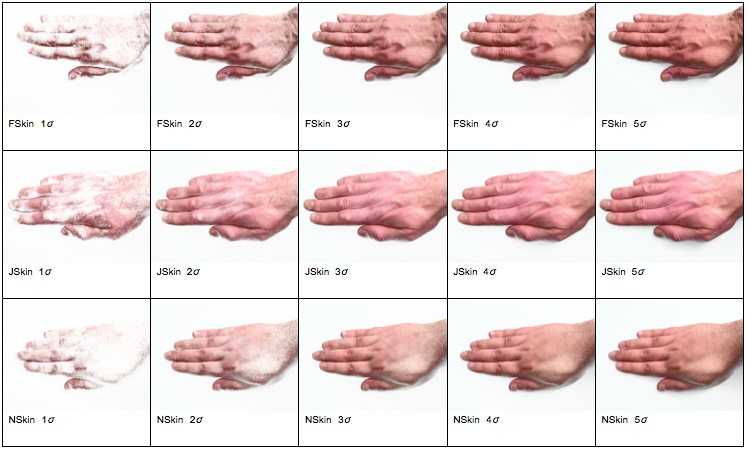
\includegraphics[width=0.95 \textwidth]{Chapter3/Figs/TransformImages.jpg} 
    \caption{ Images of hands from the three individual sets processed with the opacity given by the probability that the pixel value is skin using the simply product of Gaussians method given above.}  \label{fig:TransformImages}
\end{figure}

The probability in these images is indicated by the opacity, but as you can see from the above images, all of the skin detail is preserved, therefore all the skin information is preserved. In a normal color-space, the preservation of skin information is computationally intensive, but in the case of our bespoke color-space, it is simply the product of two 2D Gaussians, therefore finding the skin probability is a very simple function. Thus, we have not only preserved the skin information, we have produced a simplified version of a complicated computer vision task. 

It should be noted that the strict $1\sigma$ result misses some of the skin; this was expected as some histogram values lie outside the Gaussian fit, so loosening the criteria is necessary to capture all of the skin information. A $2\sigma$ or $3\sigma$ criteria should be sufficient to capture all of the skin information. Additionally, the simple implementation here does not account for unreliable white-out and black-out values, or use nearest pixel values, but this is not the final step of the algorithm. For this, we need a classifier, which will be explored in the following chapter.

\chapter{Pattern Recognition and Implementation}

% **************************** Define Graphics Path **************************

\epstopdfsetup{outdir=Chapter4/Figs/PDF/}
\ifpdf
    \graphicspath{{Chapter4/Figs/Raster/}{Chapter4/Figs/PDF/}{Chapter4/Figs/}}
\else
    \graphicspath{{Chapter4/Figs/Vector/}{Chapter4/Figs/}}
\fi


\section{Implementing the Color Space}\label{sec:ImplementingTheColorSpace}

Appendix C outlines the practical algorithm which implements the techniques developed in the previous chapters taking account of the phone characteristics. 
The resulting algorithm produces the image in the rotated color-space along with a classified image which takes 4 values relating to the probability that the pixel value is in the target color region.  

%\section{Fingertip Model}\label{sec:FingertipModel}
%
%We need an appropriate finger model so we can accurately align points on the fingertip between successive images in the video stream. We need to do this because otherwise, any difference between the frames will be overwhelmed by physical movement of the digit rather than movement of the blood inside the digit. For this reason, we target the most stable portion of the finger: the nail.
%
%A digit has two joints and three segments: the distal, the middle, and the proximal. Each segment is roughly approximated by a rectangle, and the length of each section approximately following a 2-3-5 ratio, with lengths counting from distal to proximal, and where 1 is the $\frac{3}{4}$ width of the middle segment. Our finger model then comprises of the lengths and widths of each segment, the positions of the joints (i.e. {\tiny {\tiny }}the knuckles) between each segment, the position of the tip, and a position in the model marking the point at which the digit goes out of frame.
%
%Given the width of the middle segment, we can then have an initial guess that the length of the distal segment is 1.5 times the initial width, the middle is 2.25 times that, and the proximal is 3.75 times that. Additionally, the center of the nail feature is not in the center of the distal segment, but a half unit (in our model units) away from the tip. The model can be laid out in units relative to the width of the digit.

\subsection{The Finger Shape Detection Algorithm}\label{sec:FingerShapeDetectionAlgorithm}

\subsubsection{Scale Space}\label{sec:ScaleSpace}
The images captured with the iPhone camera are extremely large, and so for the development of the algorithm, we define three scale spaces: one is the original image; two is an image size which represents the tip of the finger regardless of the distance of the camera from the finger, i.e. a scale relative to the width of the finger in the frame of the camera; three is a small image size for tracking the finger where it's freely roaming in the camera's view. We want these images to be formed without the need for re-sampling. For that reason, we restrict the choice of image sizes to those which are integer factors of the image dimensions. This is done by finding the integer factors of the original image dimensions and then selecting from those factors to scale the image. It should be noted that, to simplify point correspondences, the integer scaling from the small to medium scales is also kept.

\subsubsection{Finding the Frame Orientation}\label{sec:FindingTheFrameOrientation}
It is assumed we will not be using severed fingers, and so we know that the finger must exit the camera frame; the first step of the algorithm is then to detect which of the four edges the finger is entering from. This is done simply by finding the longest on-object path running along the frame sides. So, the algorithm starts by looking down the pixels on a frame side; when it locates a high-quaternary value, it uses the Hurdle method to find the longest path in that direction starting from that point. It continues around all four sides; the longest path found by the Hurdle algorithm is assumed to correspond to the finger entering the frame. From this, we set a frame orientation, which is the angle necessary to rotate the image such that the finger will be entering the frame from the left, and we set a direction vector pointing inwards from the frame edge found.

\subsubsection{Finding the End of the Finger Shape}\label{sec:FindingTheEndOfTheFingerShape}
Taking the longest Hurdle path on the frame edge found above, we take the middle point on that path and start a 'Run-Reach' algorithm in the direction found previously from that point. The Run-Reach algorithm proceeds as follows:

It finds a Hurdle path in the primary direction, i.e. perpendicularly away from the frame edge. At the end of the Hurdle path, it finds the Hurdle paths in the two perpendicular directions to its primary direction, i.e. parallel to the frame edge. It then finds the midpoint between the ends of the Hurdle path, and then uses that to start a new Hurdle path in its primary direction. The algorithm continues in this way until the end of the finger is found, as seen in Figure \ref{fig:FindingTheTip}.

\begin{figure}[h!]
  \centering
    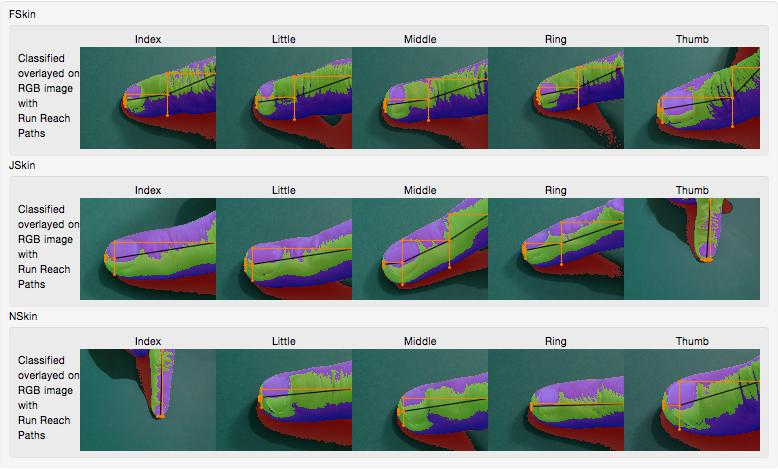
\includegraphics[width=0.95\textwidth]{Chapter4/Figs/FindingTheTip.jpg}
    \caption{Finding the End of the Finger Shape}\label{fig:FindingTheTip}
\end{figure}



\subsubsection{Filament Fill the Finger}\label{sec:FilamentFillTheFinger}
The center points found by the Run-Reach method above form a path on the finger. This is the path given to the Filament Fill method described previously. We now have a set of edge points on the digit. These edge points also have a top and bottom correspondence which, although they're not perpendicularly-opposite points on the finger, they do allow for a midpoint on the digit to be found. This can be seen in Figure~\ref{fig:FillamentFill}.

\subsubsection{Exclude Secondary Frame Edge Points and Fingertip Points }\label{sec:ExcludeSecondaryFrameEdgePointsAndFingertipPoints}
We need to exclude from the calculation of the midpoints on the digit values which are near the tip, and values which touch a second frame edge. This is because values toward the tip --- given that the finger is not necessarily perfectly horizontally-aligned --- give unreliable midpoint values because the Run-Reach path corresponds to shorter and shorter chords on a circle. Values which touch a second edge, more likely than not, do not correspond to the edge of the digit, but are simply where the digit exits the frame (for example, JSkin Middle in Figure \ref{fig:ExcludedEdgePointsAndMidlineFit}).

\begin{figure}[h!]
  \centering
    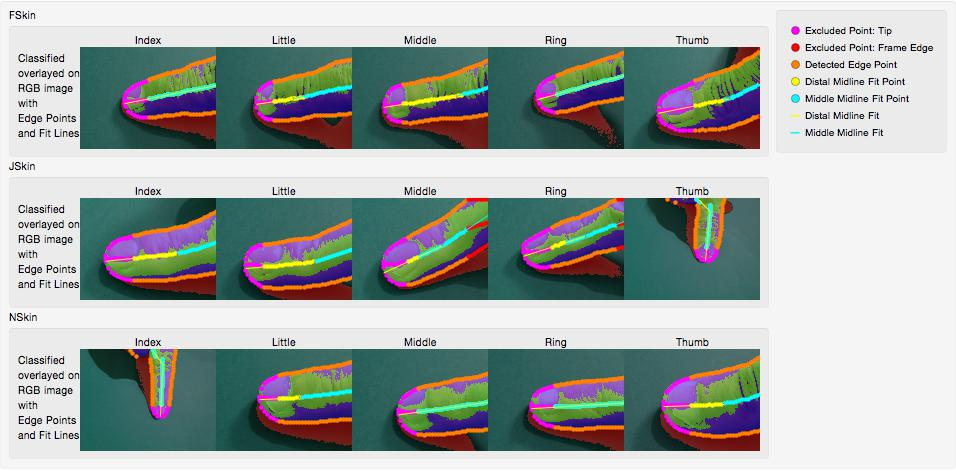
\includegraphics[width=0.95\textwidth]{Chapter4/Figs/ExcludedEdgePointsAndMidlineFit.jpg}
    \caption{Excluded Secondary Frame Edge Points and Fingertip Points, with the fit to the midline points returned by the Kink Fit algorithm.}\label{fig:ExcludedEdgePointsAndMidlineFit}
\end{figure}

To estimate which pairs of edge points correspond to points on the tip, the algorithm finds the length of the Hurdle path for all corresponding bottom-edge to top-edge points. These values are then sorted into ascending order, and then the 'Mean-Median' is taken, ensuring that the average is not affected by extreme values. The tolerance is determined by the algorithm by looking at the difference at the low and high ends of the $66\%$ range used by the Mean-Median.

\subsubsection{Kink Fit to the Finger}\label{sec:KinkFitToTheFinger}
We now have a set of reliable points at the midpoint of the finger. Because the finger is articulated, it is reasonable to assume that it may well be bent. We're interested in the action of the finger being pressed on a surface --- as a result, the finger is expected to be articulated at the distal-middle joint, but is otherwise straight. We wish to fit a function which consists of two straight-line segments to the set of reliable middle points. The fit was found using the 'Kink Fit' algorithm described in Section \ref{sec:KinkFitMethod}.

The Kink Fit algorithm as written takes a set of points where the first component is assumed to be the independent variable and the second component to be the dependent variable. However, because we haven't assumed that the finger comes into the frame from any particular direction, this can be problematic if, say, the finger comes through from the top or bottom of the frame, then the components would be in the wrong order for the Kink Fit algorithm to work. This is easily rectified by simply rotating the points into a standard orientation as if the finger is coming in from the left side of the frame. The computational effort in doing this is minimal because the number of points is small; we're not rotating the entire image, we're merely rotating a set of midline points, performing the Kink Fit algorithm, which returns a set of three points, which can then be rotated back to the original orientation.

In practice, however, the Kink Fit algorithm accepts the full set of midline points and a vector of pointers to the reliable values within that set. This allows the Kink Fit algorithm to extend out the end points of the line to the edges of the digit. Were this not the case, the end points returned would lie somewhere within the digit corresponding with the first and last reliable midline points. The result can be seen in Figure \ref{fig:ExcludedEdgePointsAndMidlineFit}.

\subsubsection{Parallel Lines Fit}\label{sec:ParallelLinesFit}
Our model of a finger assumes that the edges are parallel to each other. Since we have a line which runs through the center of the finger, we can now calculate the distance of the edge points to that line. These distances can be classified as good edge points if they're parallel to the central line. Whether they are parallel is determined by finding the Mean-Median distance from the central line to the edge points using a $50\%$ interval in the distal portion, because it is expected that up to half the points may be in the distal segment, maybe on the tip, and a $75\%$ confidence interval in the middle segment, because we expect fewer than $\frac{1}{4}$ of the edge points to be anomalies. The points are then classified as good if they are of Mean-Median distance from the central line. It should be noted that we consider both the top and bottom edges when calculating the Mean-Median distance. This technique successfully removes anomalies which are not parallel to the central line.

There is one final step: the points which are classified as good edge points are used to find a linear fit which is parallel to the central line. Finally, the width of the distal and the middle segments is calculated by finding the distance between these parallel lines. This can be seen in Figure \ref{fig:ParallelFit}.

\begin{figure}[h!]
  \centering
    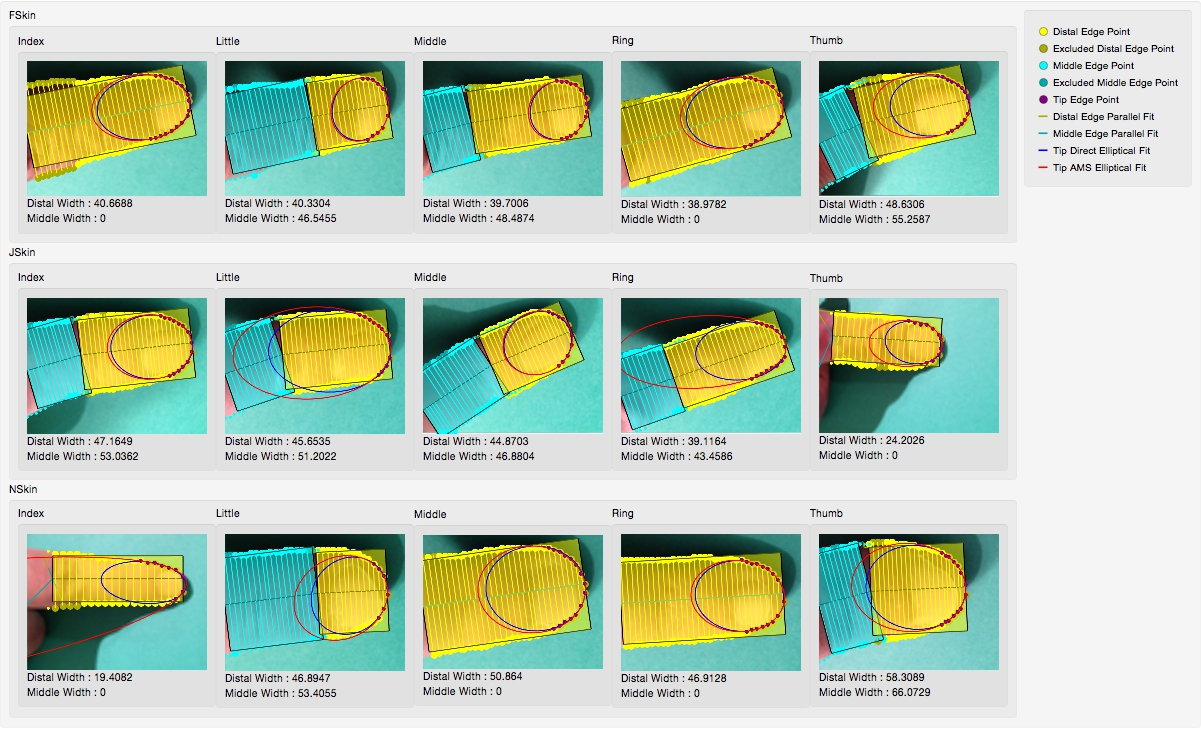
\includegraphics[width=0.95\textwidth]{Chapter4/Figs/ParallelFit.jpg}
    \caption{Initial shape-fitting stage, with the Kink Fit, midline, and Parallel Edge fit, with AMS and Direct elliptical fits to the tip.}\label{fig:ParallelFit}
\end{figure}

\subsubsection{Set the Scale Space}\label{sec:SetTheScaleSpace}
We wish to set the mid-scale such that the number of pixels across the distal segment is close to a chosen target value. As mentioned in the scale space subsection \ref{sec:ScaleSpace} we are restricting the choice of scales to integer factors of the original and integer multiples of the small scale. For the iPhone images the factors are:
\begin{align}
scale &= 2^{-i} 3^{-j} 17^{-k}  & i &\in \{0,1,2,3,4\} 
&  j &\in \{0, 1\} 
& k &\in \{0, 1\}
\end{align}

The small scale space is made using the largest number of small factors as possible to achieve the desired image size. This gives the greatest flexibility in scaling the mid-size.
\begin{table}[h]
\centering
\begin{tabular}{|cc|cc|c|c|c|c|c|l|}
\cline{5-10}
\multicolumn{3}{c}{ }  & & $0$ & $1$ & $2$ & $3$ & $4$ & i\\
\cline{1-10}
k & $k_{scale}$ &j & $j_{scale}$ & $1$ & $\frac{1}{2}$ & $\frac{1}{4}$ & $\frac{1}{8}$ & $\frac{1}{16}$ & $i_{scale}$\\
  \hline \hline
\multirow{4}{*}{$0$} & \multirow{4}{*}{$1$} & \multirow{2}{*}{$0$} & \multirow{2}{*}{$1$} & 
 2448 & 1224  &  612  & 306  & 153 & w \\
  &  &  & & 
  3264  & 1632  & 816  & 408  & 204  & h\\
  \cline{3-10}
 &  & \multirow{2}{*}{$1$} & \multirow{2}{*}{$\frac{1}{3}$} & 
 816  & 408  & 204  & 102  & 51  & w \\
 &  &  & & 
  1088  & 544   & 272  & 136  & 68  & h \\
\hline 
  \hline
\multirow{4}{*}{1} & \multirow{4}{*}{ $\frac{1}{17}$ } & \multirow{2}{*}{$0$} & \multirow{2}{*}{$1$} & 
 144  & 72  & 36  & 18  & 9 & w \\
 &  & & & 
  192  & 96  & 48  & 24  & 12  & h \\
    \cline{3-10}
 &  &  \multirow{2}{*}{$1$} & \multirow{2}{*}{$\frac{1}{3}$} & 
 48  & 24   & 12  & 6   & 3 & w \\
   &  &   & & 
  64  & 32  & 16  & 8  & 4  & h \\
\hline 
\end{tabular}
\caption{The image pixel dimensions for all possible integer factor scalings.}
\end{table}

So for a chosen small scale $S_s = 2^{-3} 3^{-1}$, a distal width in the small scale $w$ and a minimum distal width in the medium scale $w_m$. 
Finding  $i_m$ and $j_m$ which minimise $i_m + \frac{\log(3)}{\log(2)} j_m$  and which satisfy  $2^{-i_m} 3^{-j_m} - \lceil \frac{w_m}{w} \rceil \ge 0$, $i_m\le i_s$ and $j_m \le j_s$ determines the medium scale space.

\subsubsection{Modelling the Fingertip}\label{sec:ModellingTheFingertip}
\begin{figure}[p!]
  \centering
  \noindent
  
  \begin{tabular}{cc}
  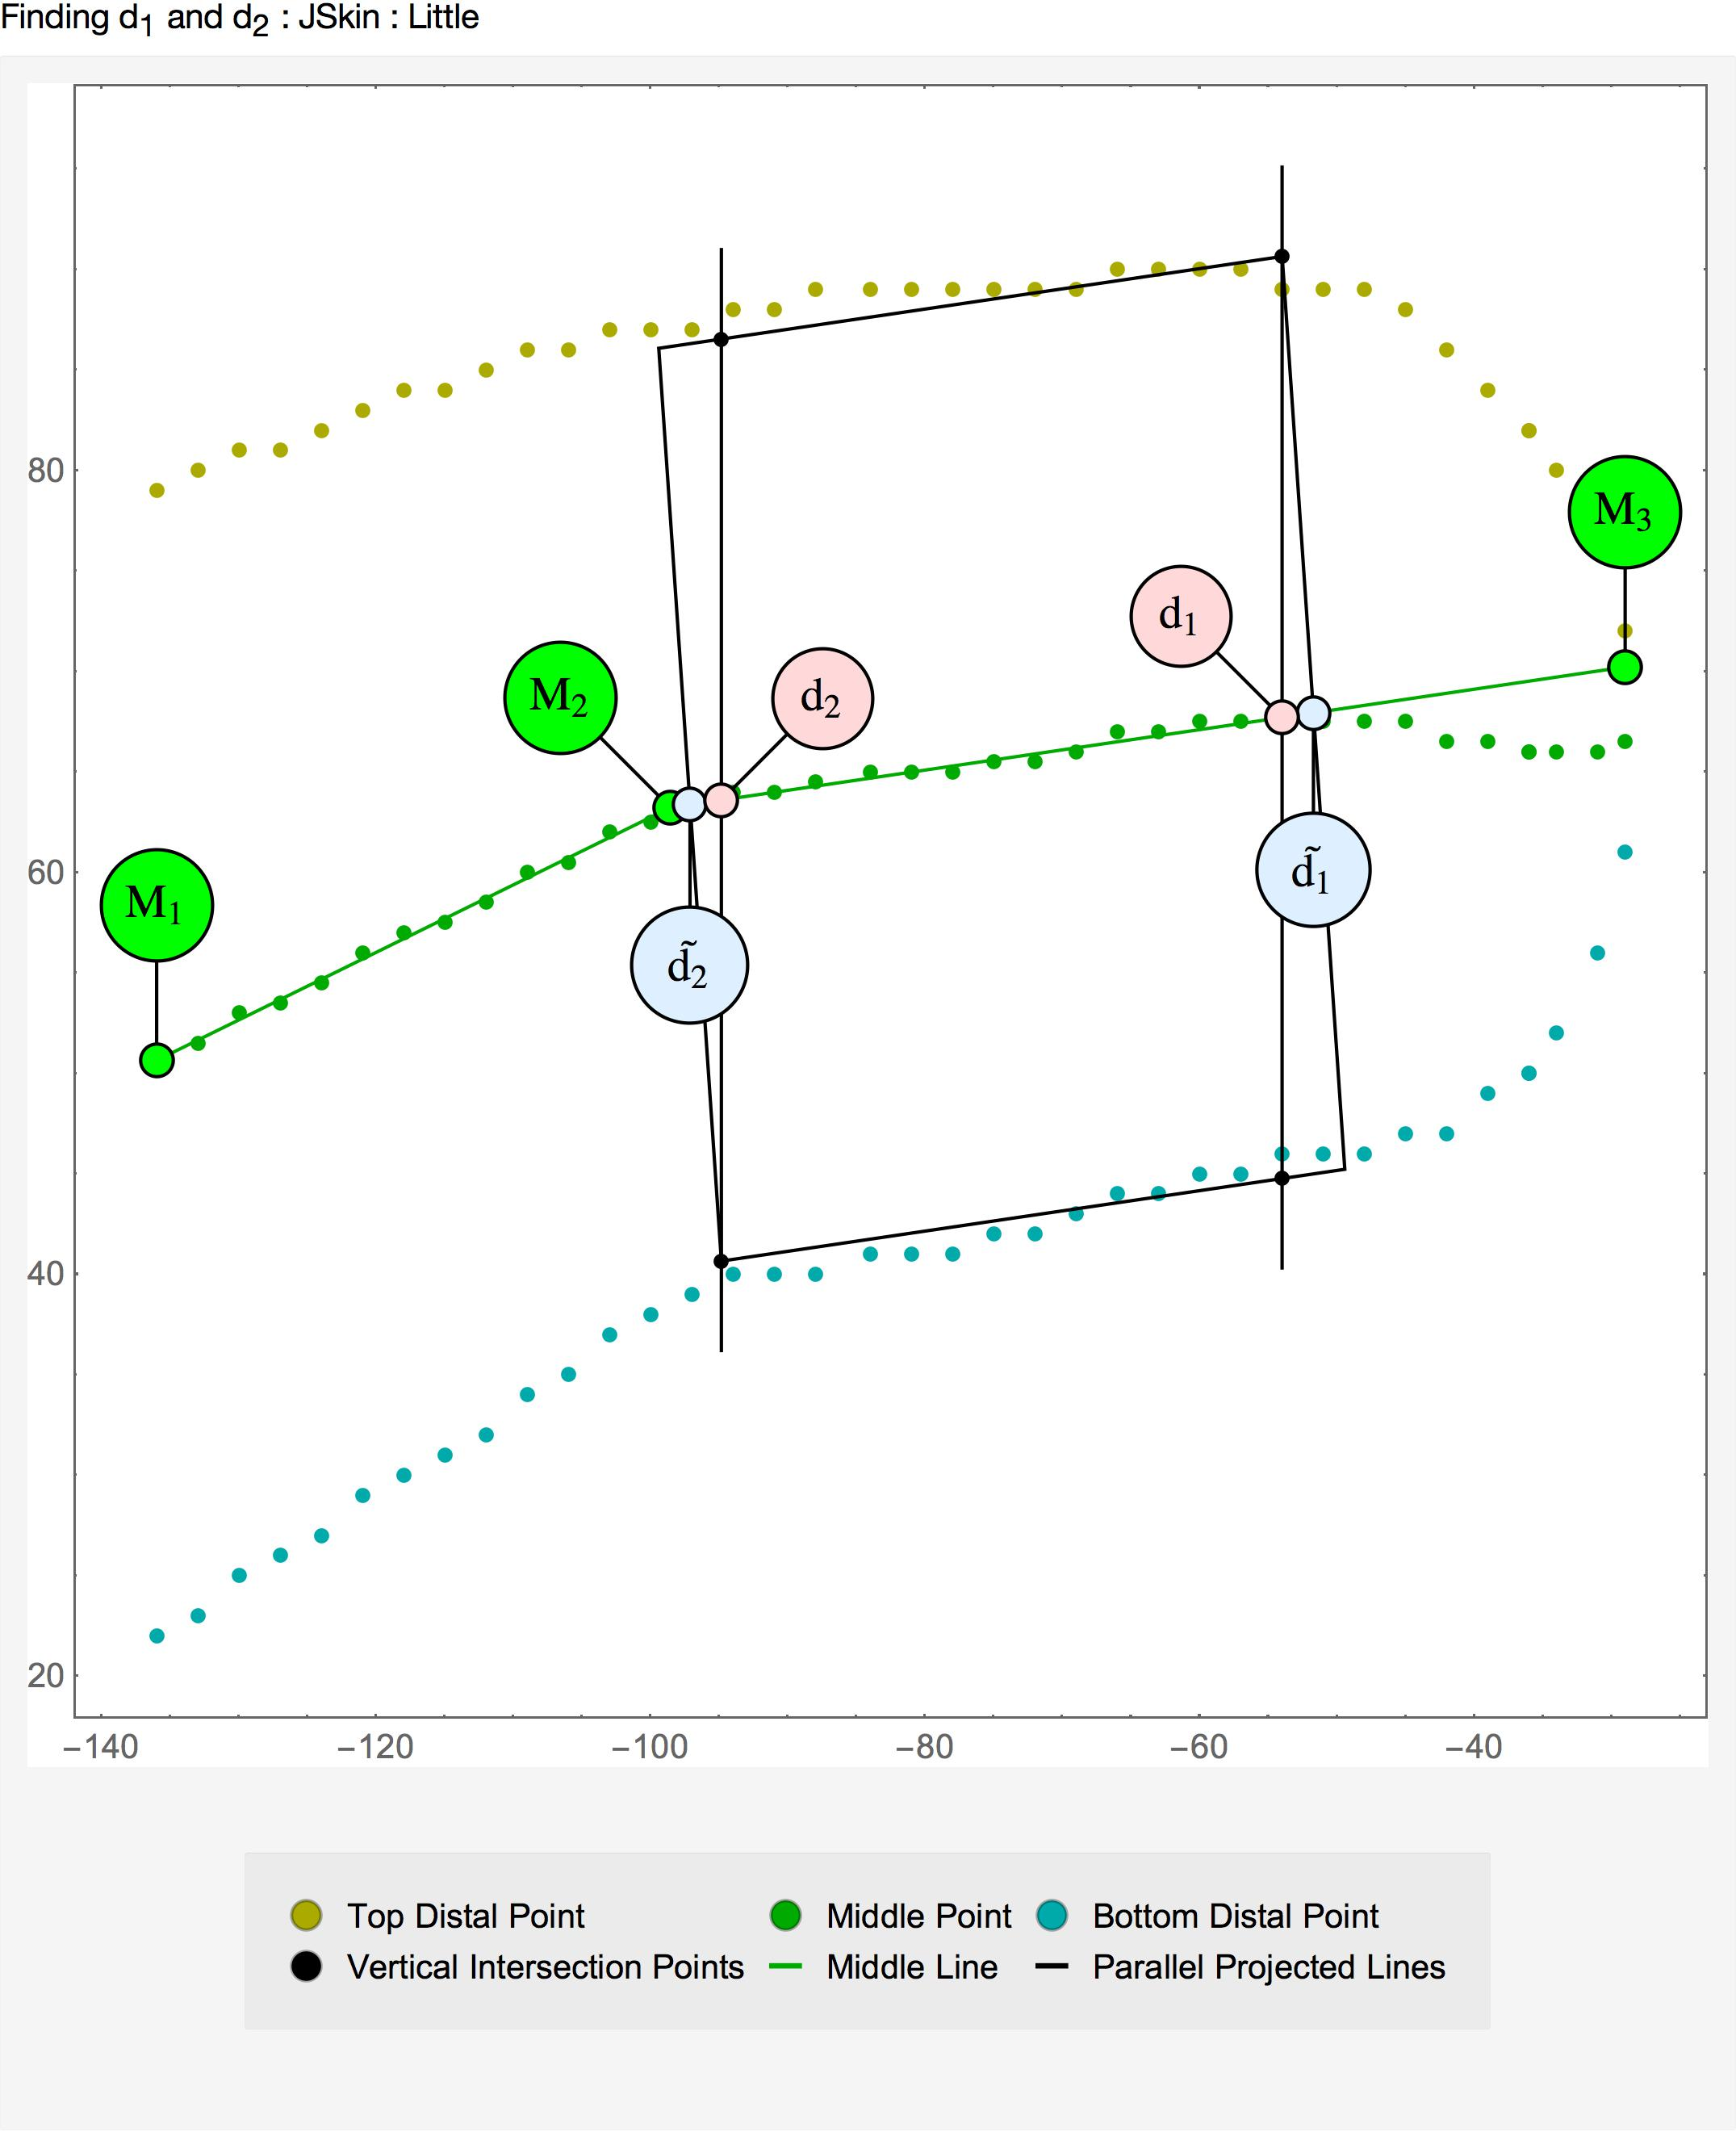
\includegraphics[width=0.45\textwidth, height=0.5\textwidth]{Chapter4/Figs/Model_FindingD1AndD2_JSkin_Little.jpg} &
    \parbox[b][0.5\textwidth][s]{0.55\textwidth}{
   \textbf{a) Determining $d_1$ \& $d_2$} --- We have a midline which is given as two points $M_2$ \& $M_3$; one somewhere on the digit ($M_2$), and the other at the tip ($M_3$). If the finger were straight in the frame, then $d_1=\tilde{d_1}$ and $d_2=\tilde{d_2}$ could easily be found by finding the points on that line. However, the fact that the digit can be presented at an angle means that the edge points vertically above and below the point on the midline may include part of the curved tip. This has the effect of making these midpoints diverge from the midline of the digit. This can be corrected by adjusting with half the gradient of the midline $\delta\:mid$ to the ratios. \begin{equation*}distance \:on \:line = (\frac{1}{2} + \left\lvert\frac{1}{2}\delta\:mid\right\lvert) w\end{equation*} \vfill
    } \\ 
    \parbox[b][0.5\textwidth][s]{0.45\textwidth}{
             \textbf{b) A New Midline Fit} --- We take the set of midline points, extract the subset which lies between $d_1$ and $d_2$, and then apply a straight line fit to these points. The origin is the fit evaluated at the $x$ component of $d_2$, and we determine an orientation $\theta$, which is $\arctan$ the gradient of the linear model. \vfill
        } &
        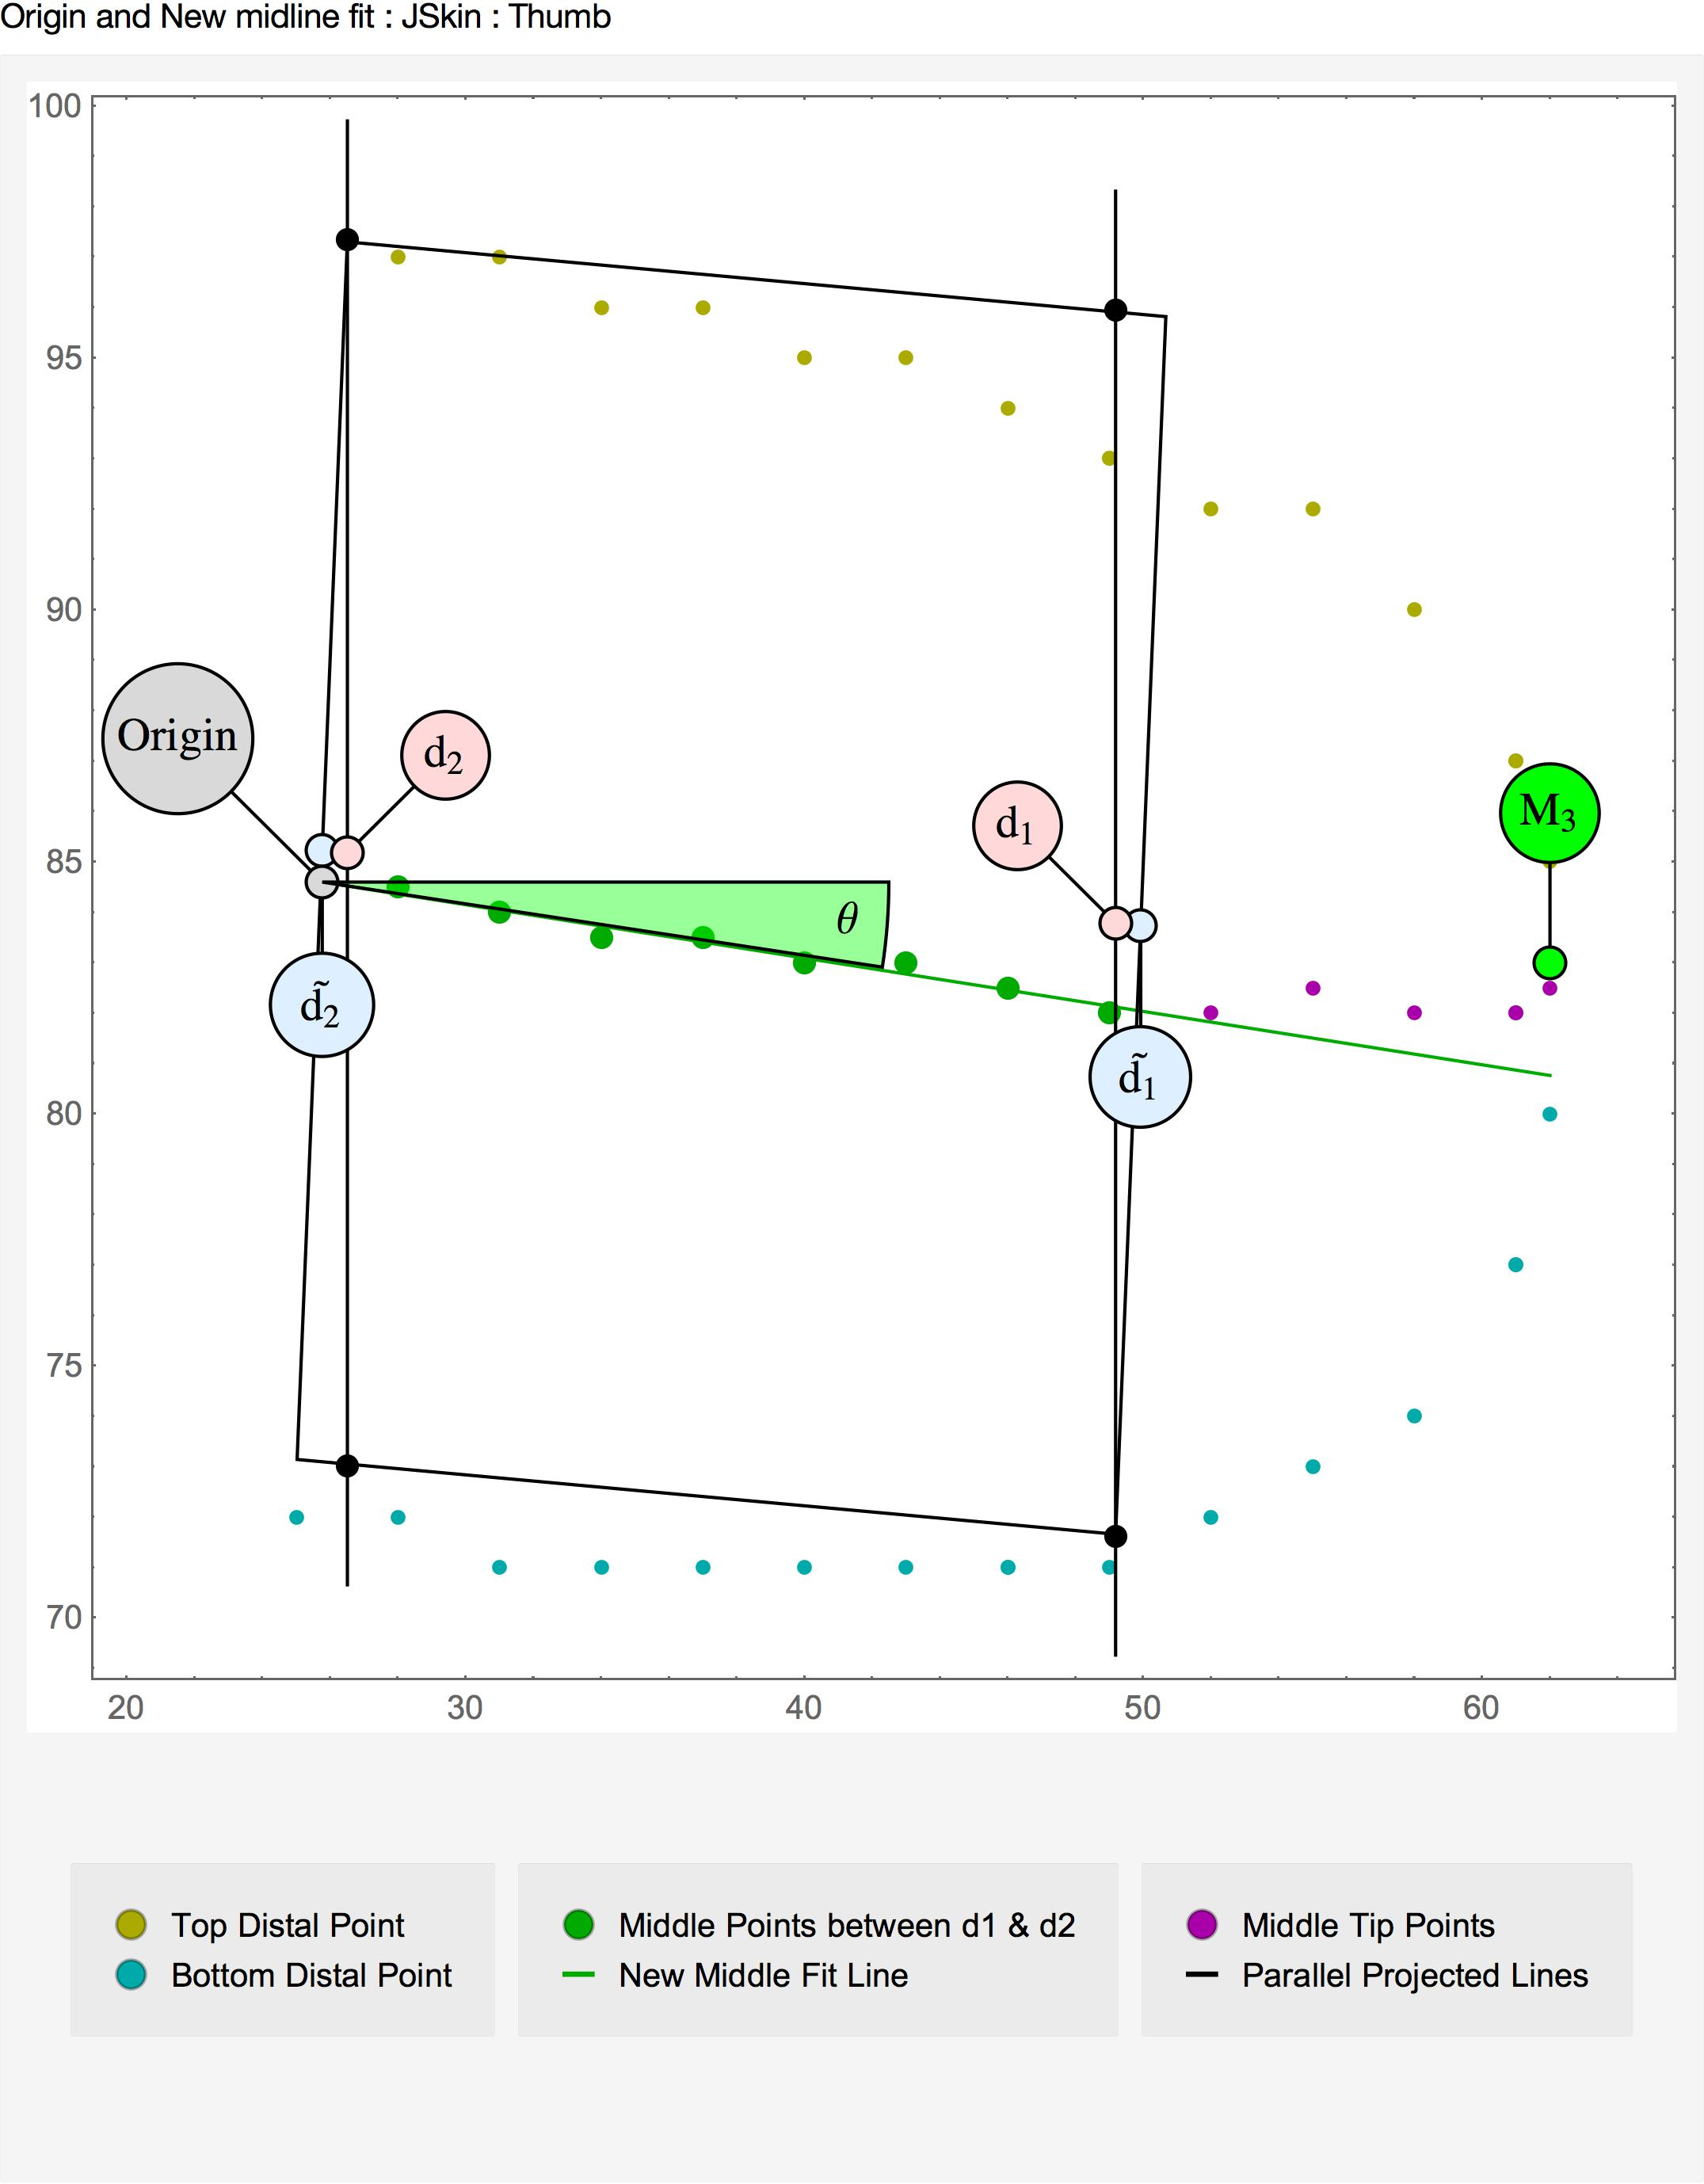
\includegraphics[width=0.55\textwidth, height=0.5\textwidth]{Chapter4/Figs/Model_Midline_JSkin_Thumb.jpg} 
    \\ 
   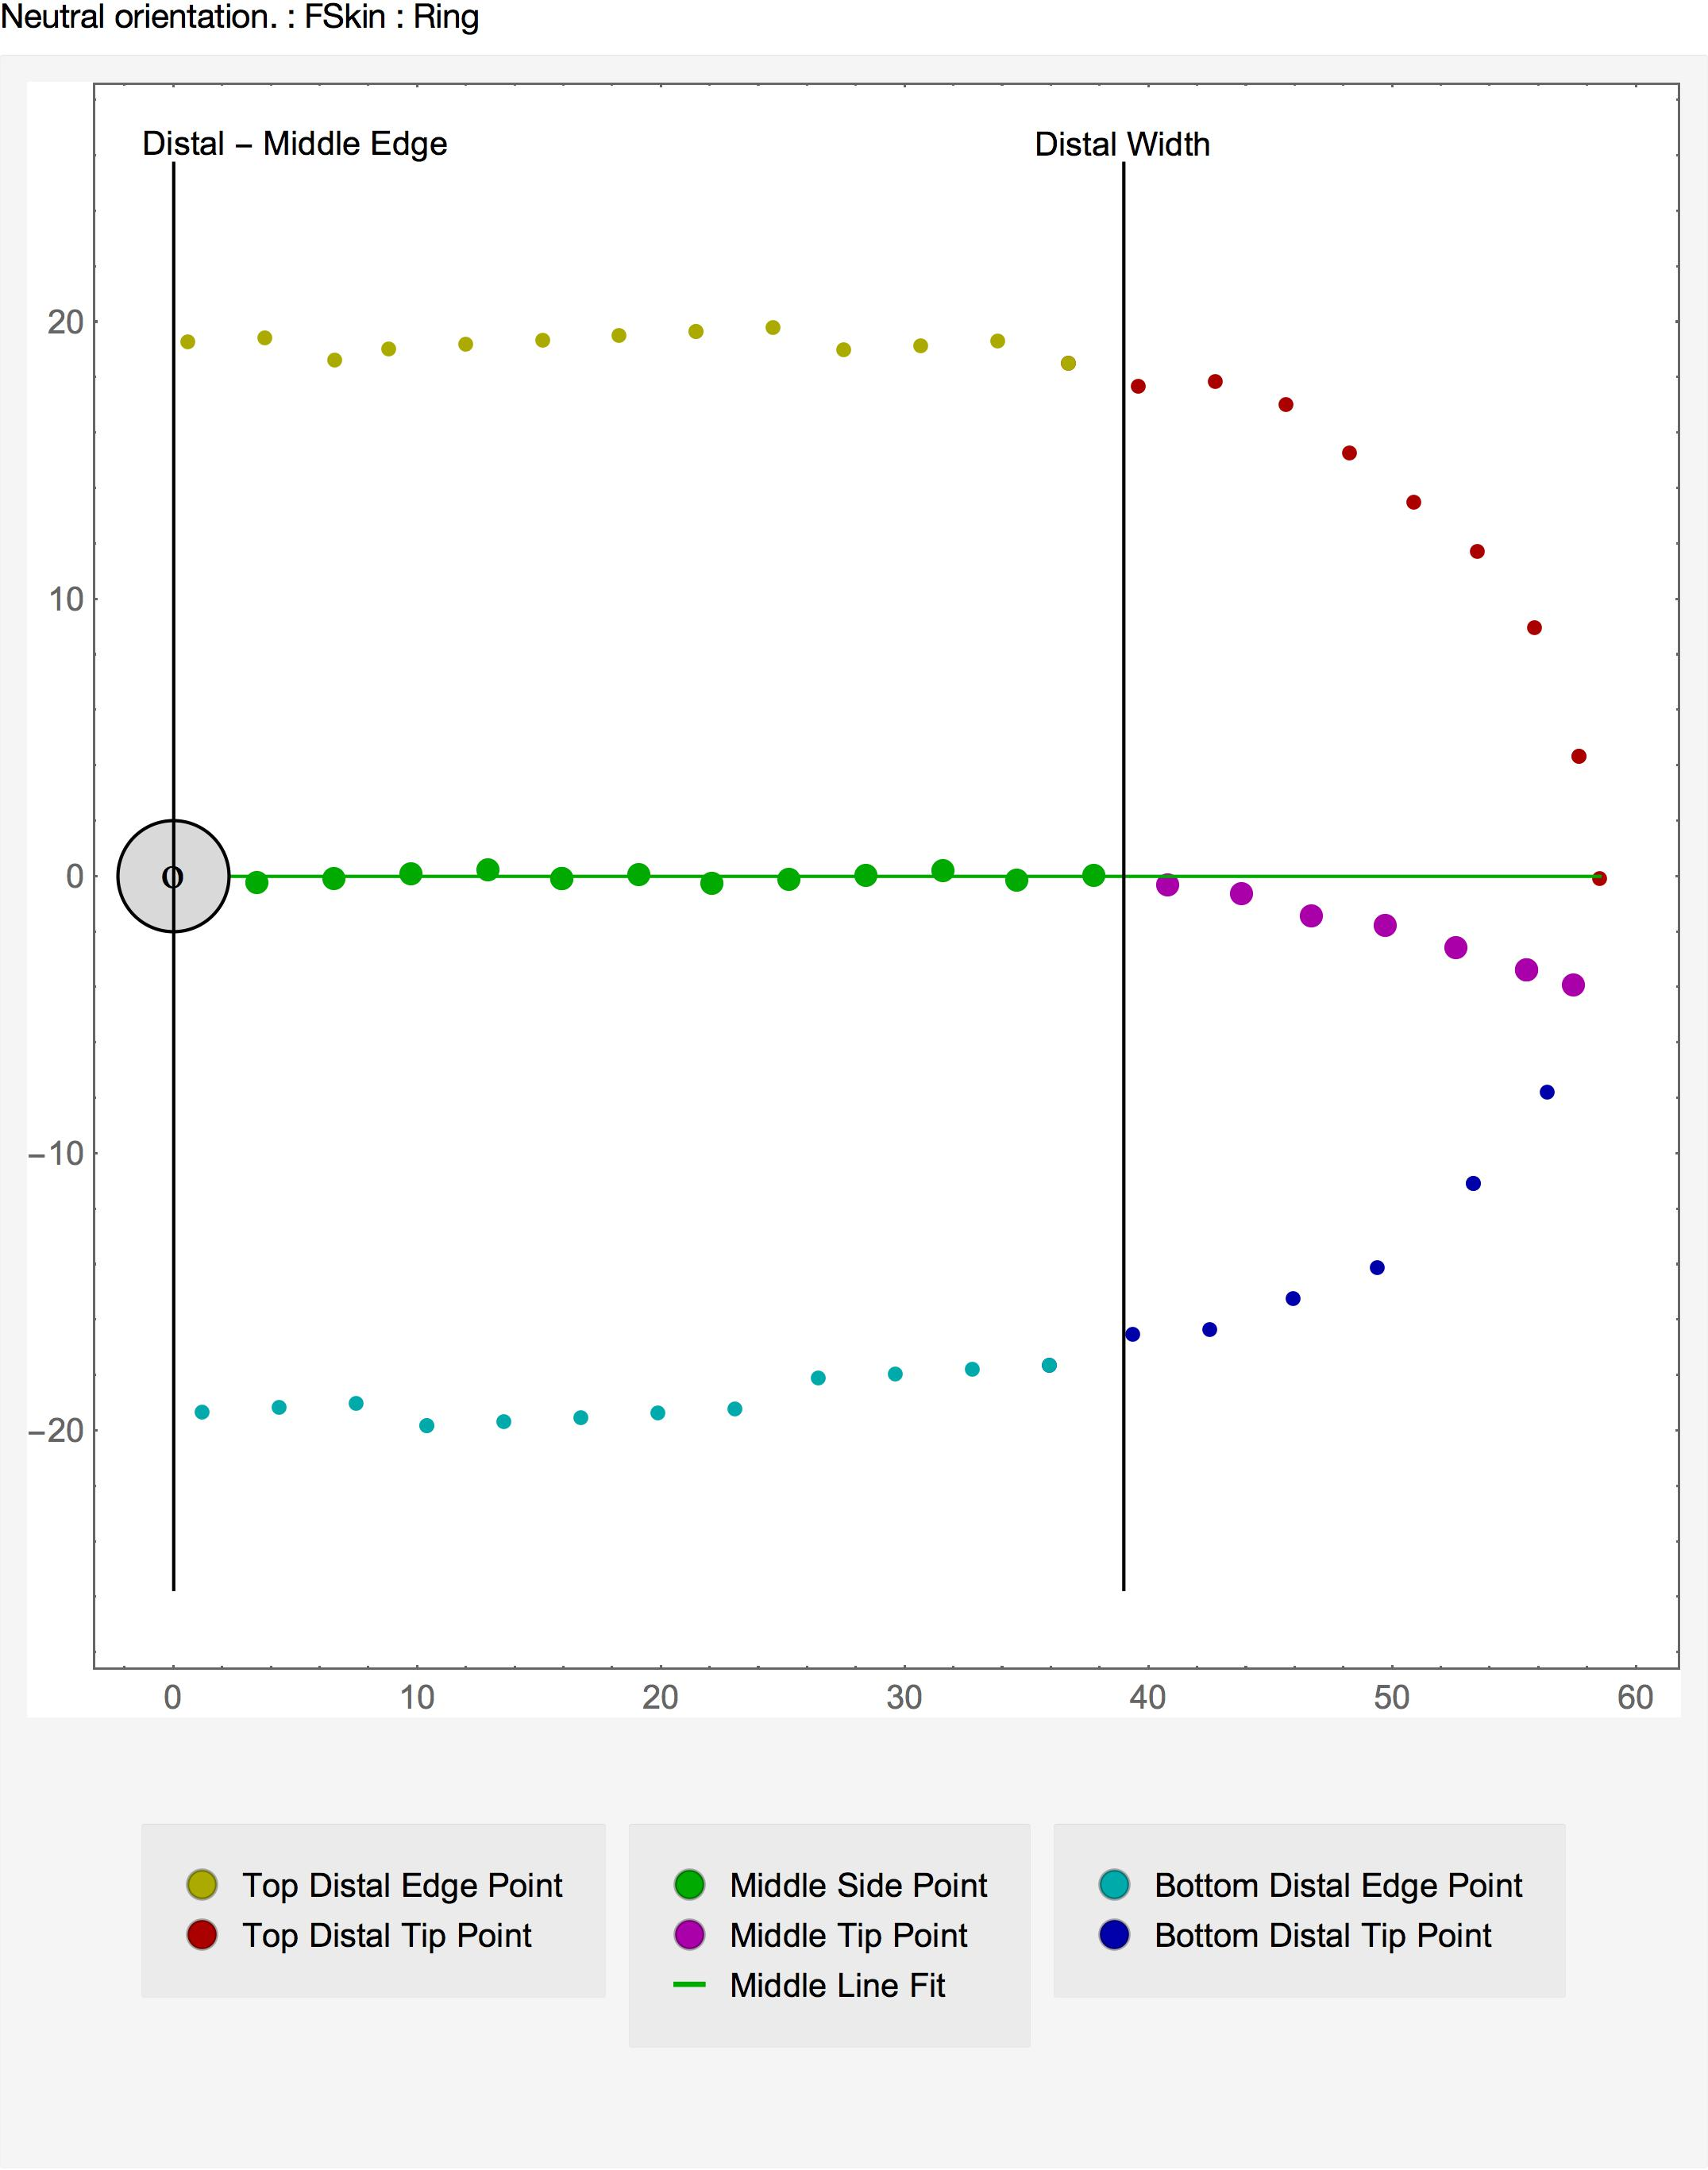
\includegraphics[width=0.45\textwidth, height=0.5\textwidth]{Chapter4/Figs/Model_NeutralCoords_FSkin_Ring.jpg} &
    \parbox[b][0.5\textwidth][s]{0.55\textwidth}{
         \textbf{c) Determine the Neutral Coordinates} --- We move all the points --- the top and bottom edges, and the midline points --- and we translate to the new origin. Then, we rotate by $-\theta$. This we call the "neutral coordinates", as the tip is aligned with its midaxis lying on the $x$ axis. These points are separated at one distal width from the tip; a Trapezian fit is applied to one set of points, and an Elliptical fit is applied to the other. As a refinement to this, although the linear fit is applied as in the Trapezian section, the algorithm then looks at the points beyond and before the one distal width region; if they're consistent with the fit, then they are considered still part of the straight edge. The Elliptical fit is applied as discussed previously. \vfill
    }
    \end{tabular}\\
    \phantomcaption
\end{figure}
\addtocounter{figure}{-1}

\begin{figure}[p!]
\ContinuedFloat
\centering
\begin{minipage}[t]{1\textwidth}
\begin{wrapfigure}{l}{0.5\textwidth}
  \begin{center}
    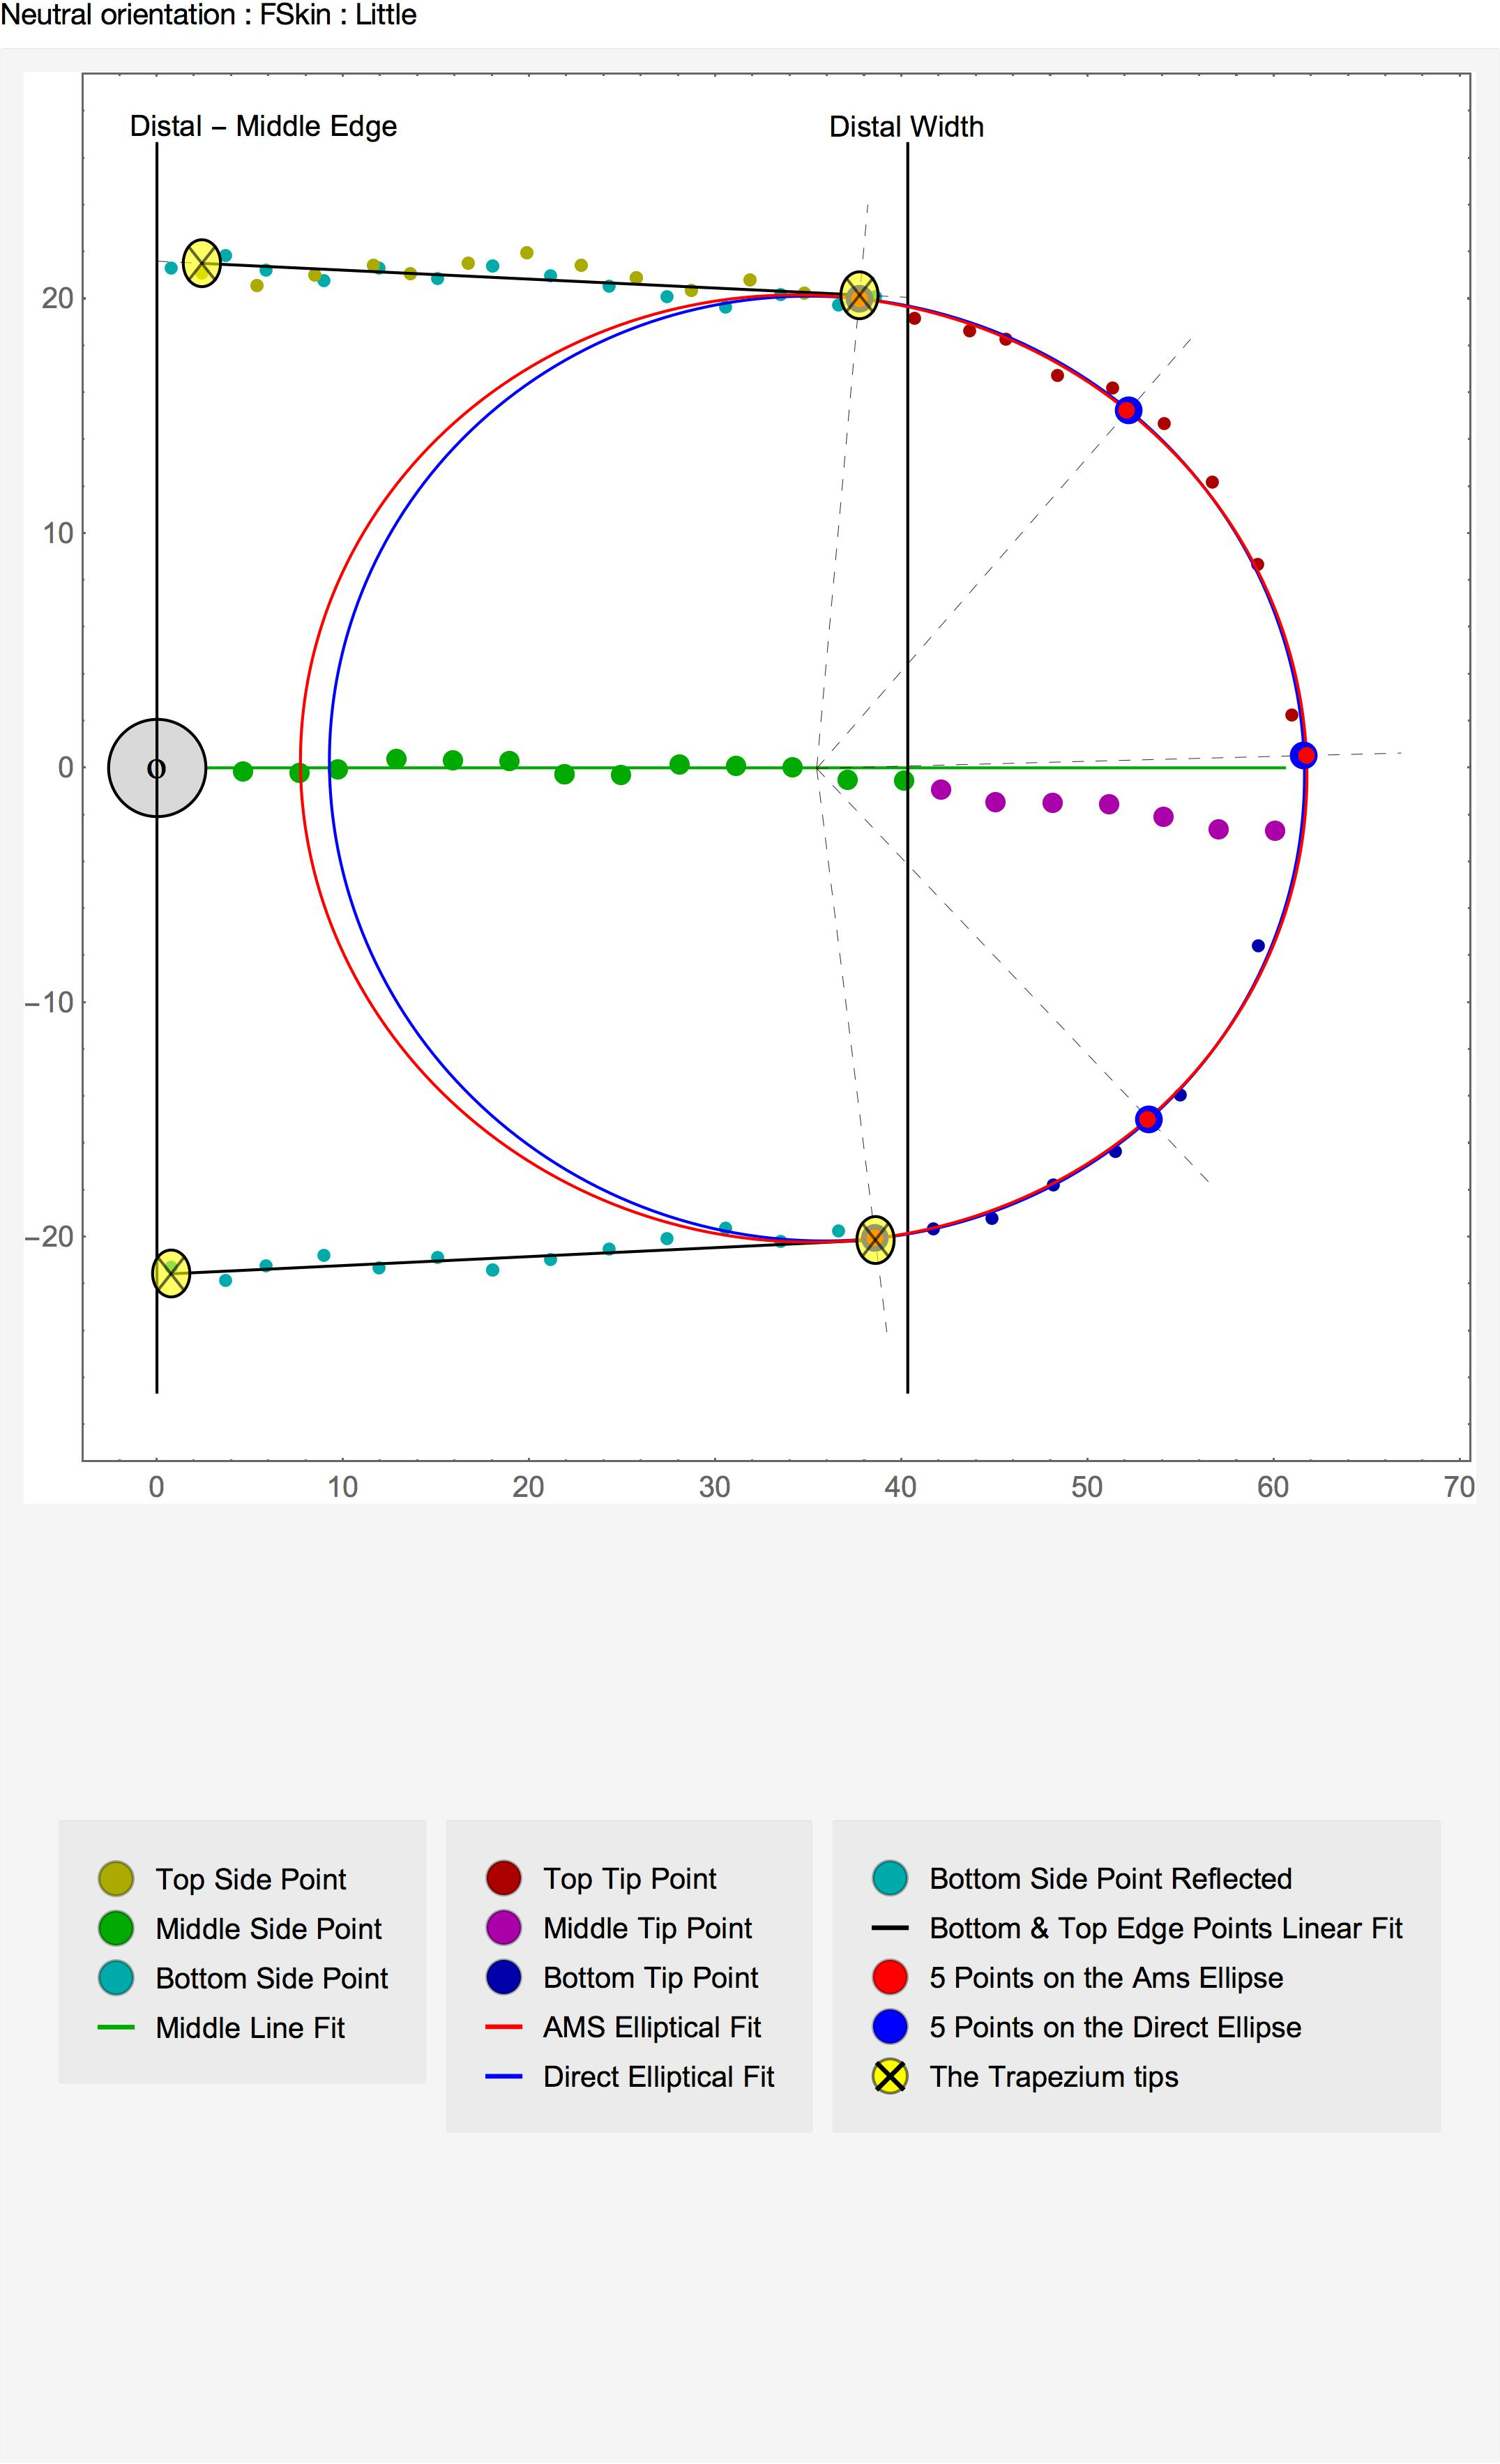
\includegraphics[width=0.5\textwidth]{Chapter4/Figs/Model_ShapeFitting_FSkin_Little.jpg}
  \end{center}
  \phantomcaption
\end{wrapfigure}
         \textbf{d) Fitting the Shapes} --- The comparison between the elliptical fit methods is done by looking at the distance from the front two points on the trapezium to the edge of the ellipse, and the best of these is chosen. Unfortunately, this is often not sufficient to make the ellipse join with the trapezium exactly because further on in the algorithm, these shapes will be used to perform a mask; we want to avoid introducing artefacts which could be interpreted as features. So, we wish to remove these discontinuous intersections between the ellipse and the trapezium. In order to do this, we choose three points on the Elliptical fit and the two front points of the trapezium, thereby making a set of five points, and we pass these through the direct Elliptical fit algorithm. It should be noted that five points is what is required to completely define an ellipse; there is only one ellipse which will pass through five points.
    \end{minipage}
    \subfloat{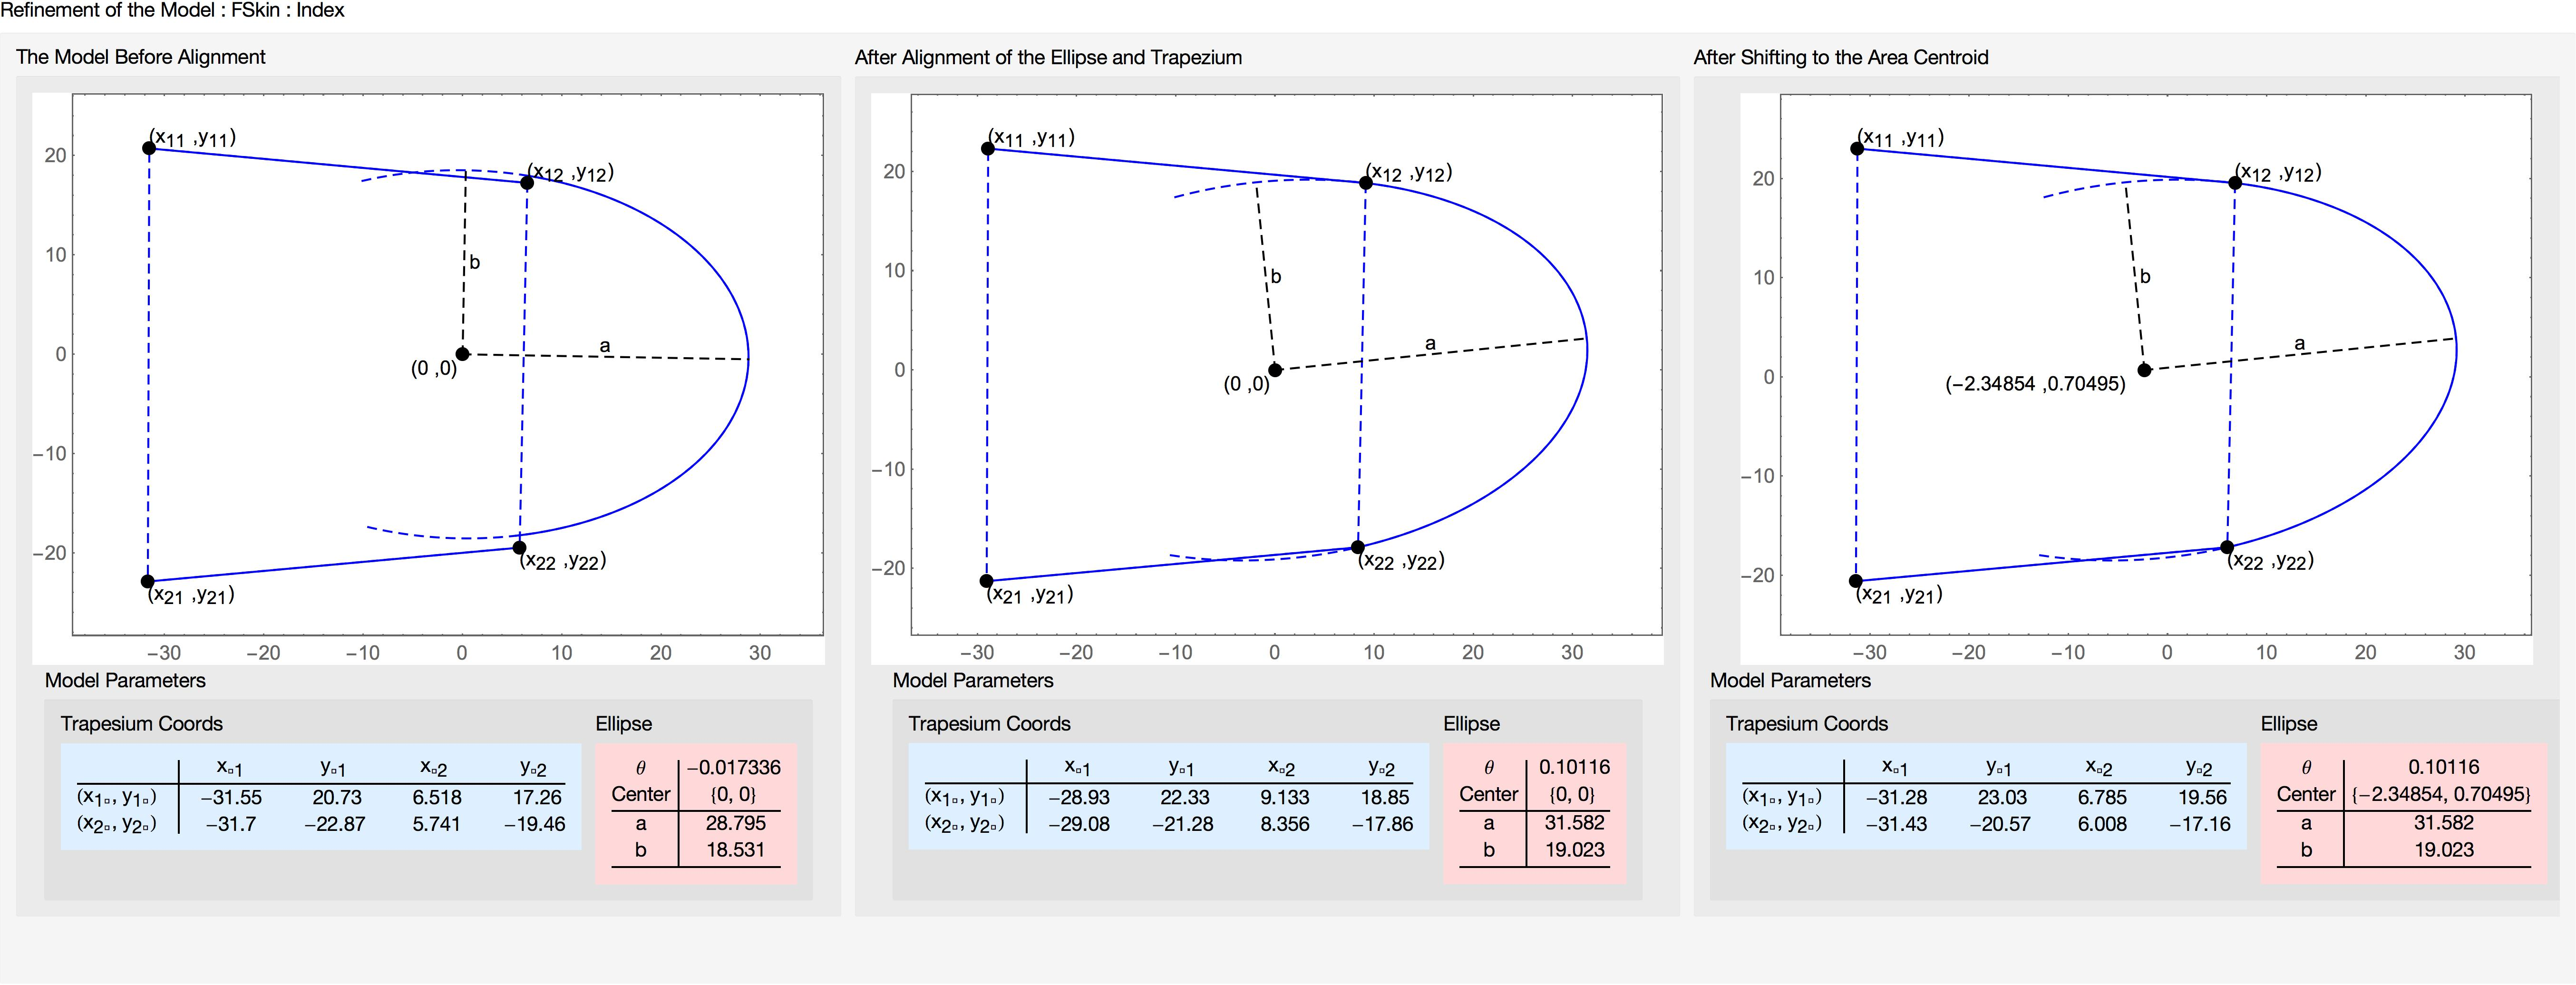
\includegraphics[width=0.99\textwidth]{Chapter4/Figs/Model_Finalizing_FSkin_Index.jpg}}\\
    \begin{minipage}{0.95\textwidth}
         \textbf{e) Finalizing the Model} --- The coordinates for the ellipse and the trapezian are adjusted so that the origin is at the center of the ellipse, and the ellipse has zero rotation. The reason for this is that it makes calculating the distance from the edges of the ellipse easier. So, now when we apply the model to the image, all that's required is a position --- which is the position of the center of the ellipse --- and an orientation about that position. 
    \end{minipage}
    \caption{The Fingertip Model Algorithm.}\label{fig:ModelingFingertip}
\end{figure}

Having determined a measure of the width of the distal portion of the fingertip allows for a more robust model of the fingertip to be determined. This is because the measurement of the distal width is far more reliable than the distal length which has so far been determined, as the distal length has been found by evaluating where the "kink" of the midline points lies. For example, if the distal joint is un-flexed, the knuckle portion will be overlooked entirely, as seen in Figure \ref{fig:ParallelFit}. It turns out that the average anatomical ratios of the distal,  middle, and  proximal lengths $2:3:5$ and the width $w$ to distal length $l_{d}$ ratio $2 : 3$  is a far more reliable method of determining the distal length $l_{d} = 1.5 w$.

From the kink fit, we have a midline, which is specified by three points. We now determine two points on this line, which are $\frac{1}{2}$ the distal width ($d_1$) and $1\frac{1}{2}$ the distal width from the tip ($d_2$). So the midline point that lies between the two points can now be taken to correspond to the straight-edged section of the distal portion of the finger. These points are passed to the Trapezian Fit method (\ref{sec:TrapezianFit}), and the points which lie between the tip and the point half the distal width from the tip are passed to the Elliptical Fit (\ref{sec:EllipticalFitMethod}). The ellipse is adjusted to correspond with the two near vertices of the Trapezian; the result can be seen in Figure \ref{fig:ModelingFingertip}.

\begin{figure}[h!]
  \centering
    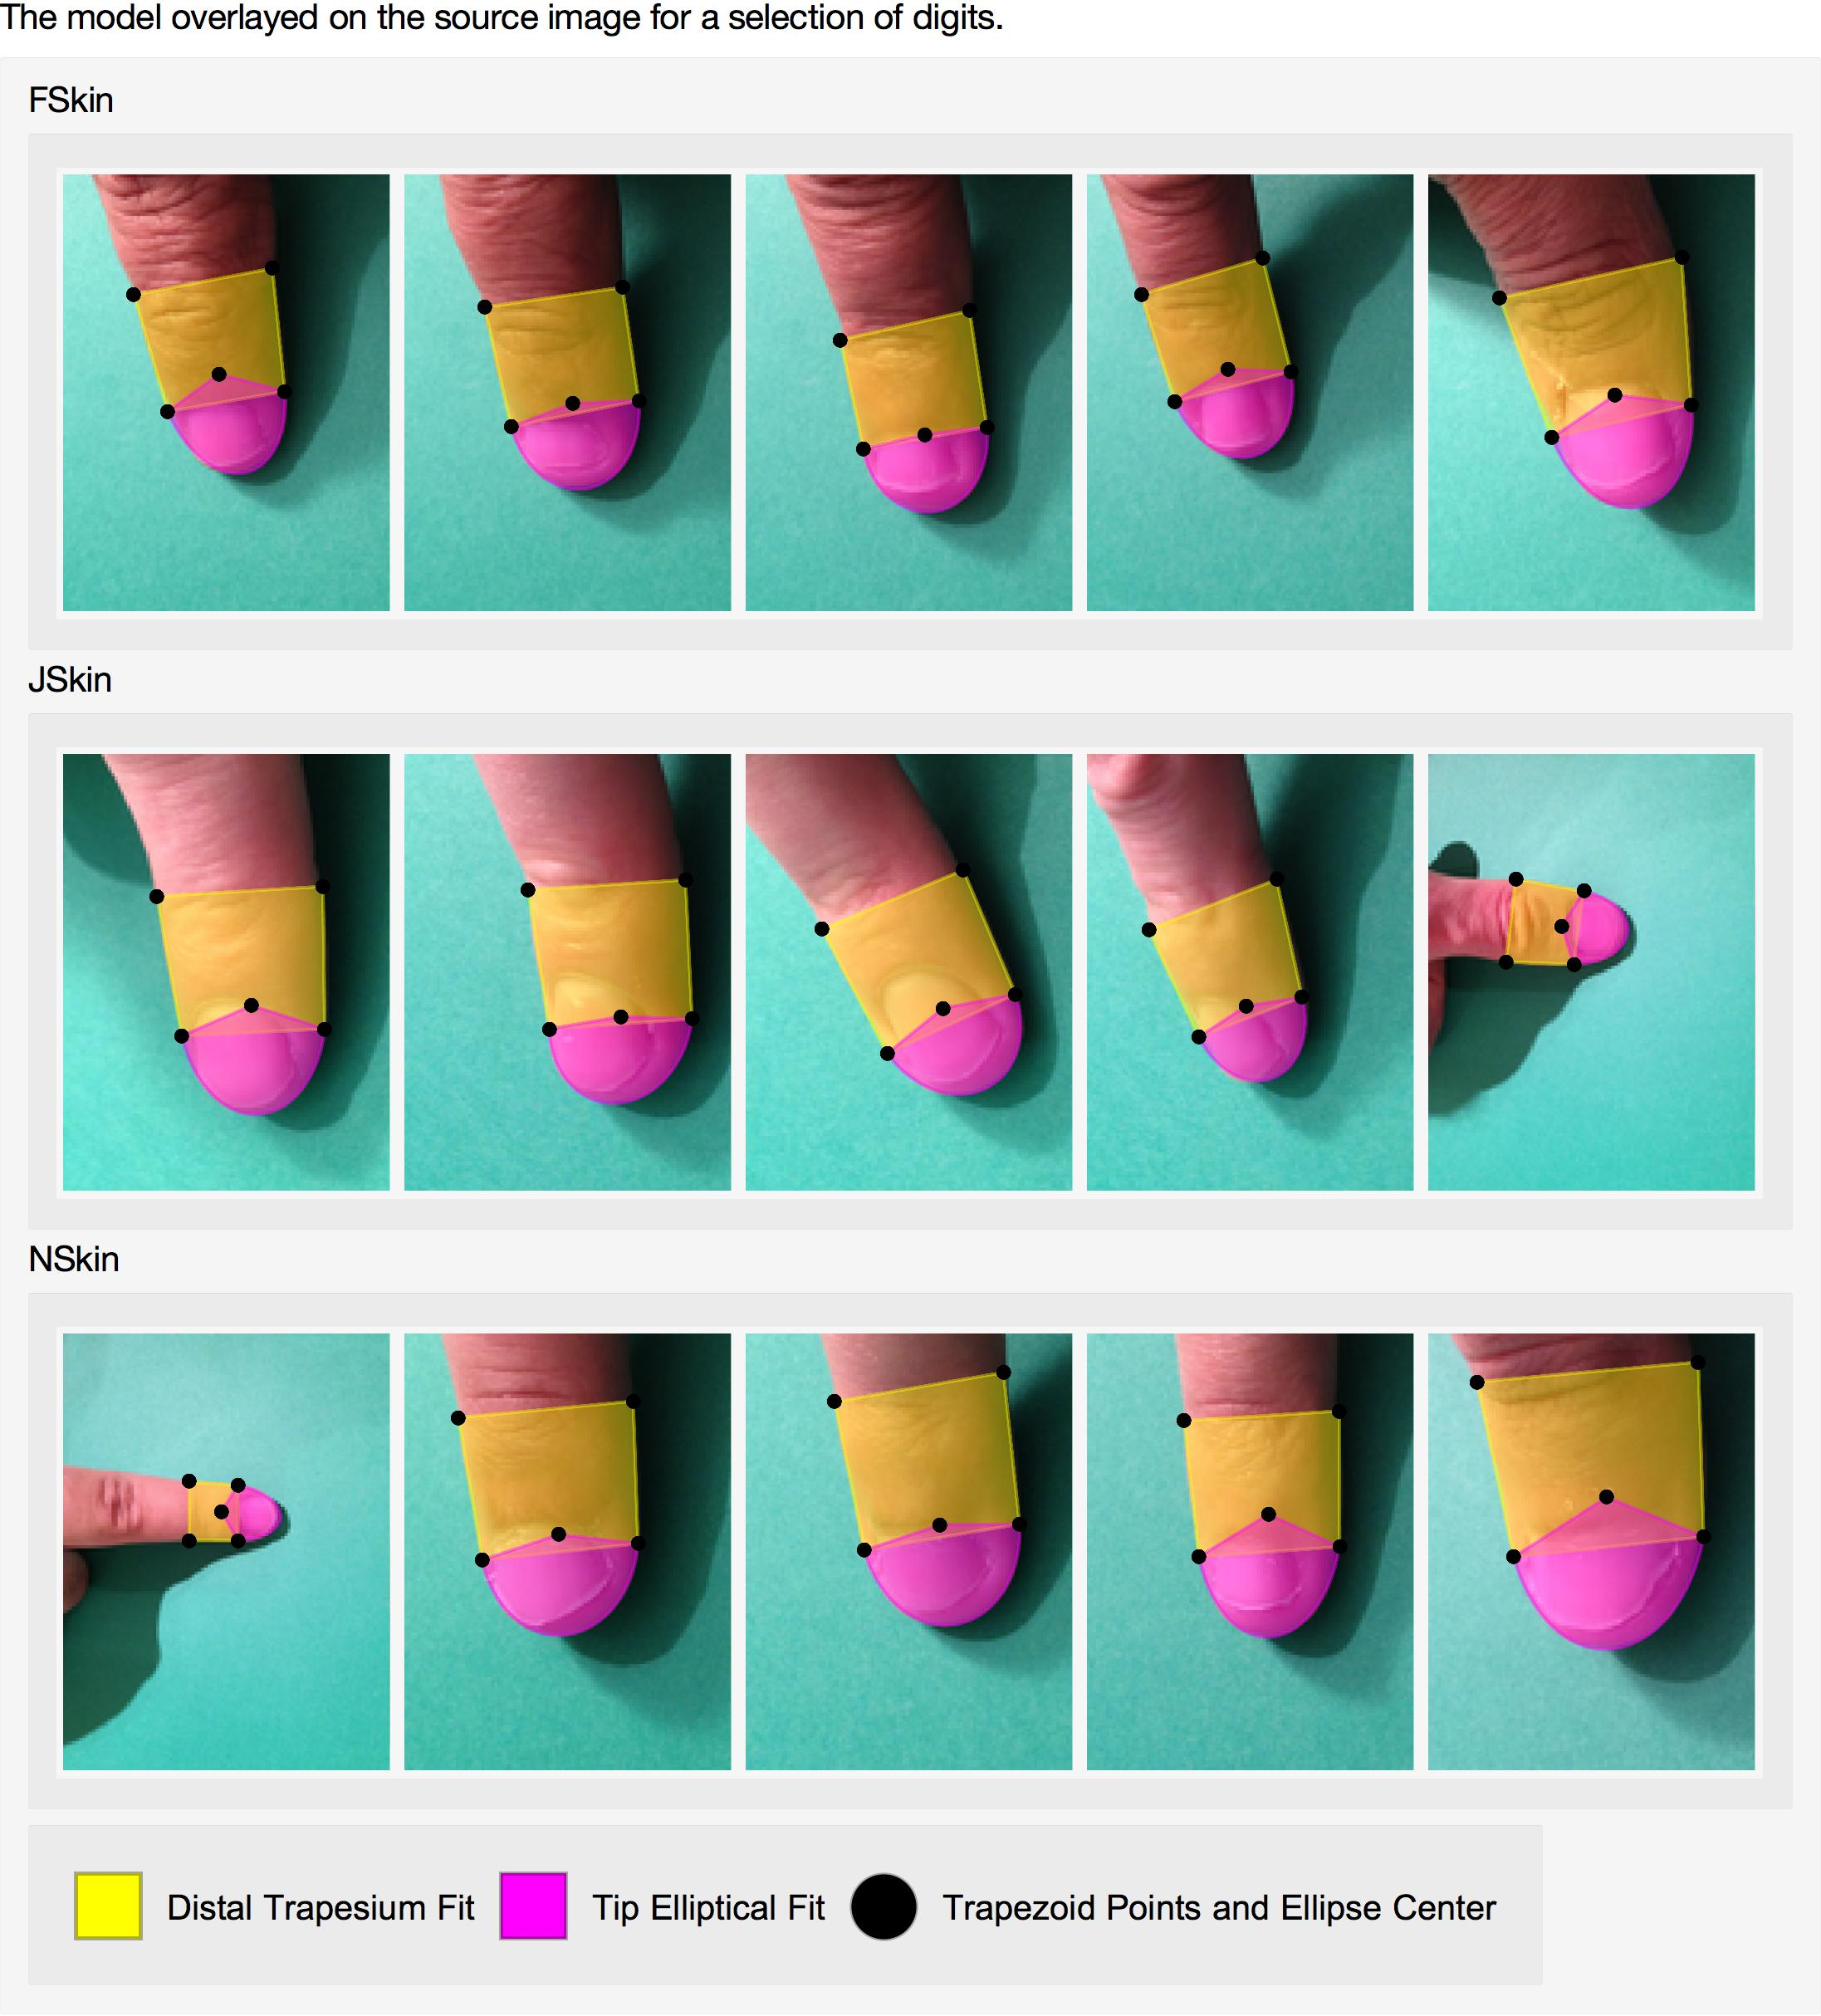
\includegraphics[width=0.99\textwidth]{Chapter4/Figs/Model_Overlayed.jpg}
    \caption{The models overlayed on the source images.}\label{fig:FingertipModelResult}
\end{figure}

Overlaying the model on its source image shows that the application of the model actually only requires a position and orientation, because we assume that the camera is positioned such that the digit presents at the same scale when in contact with a surface throughout the frame; we're not accounting for perspective effects in this simple application.
The model can be seen overlayed on the selection of digits for three individuals in Figure \ref{fig:FingertipModelResult}.


\begin{sidewaysfigure}[h!]
  \centering
    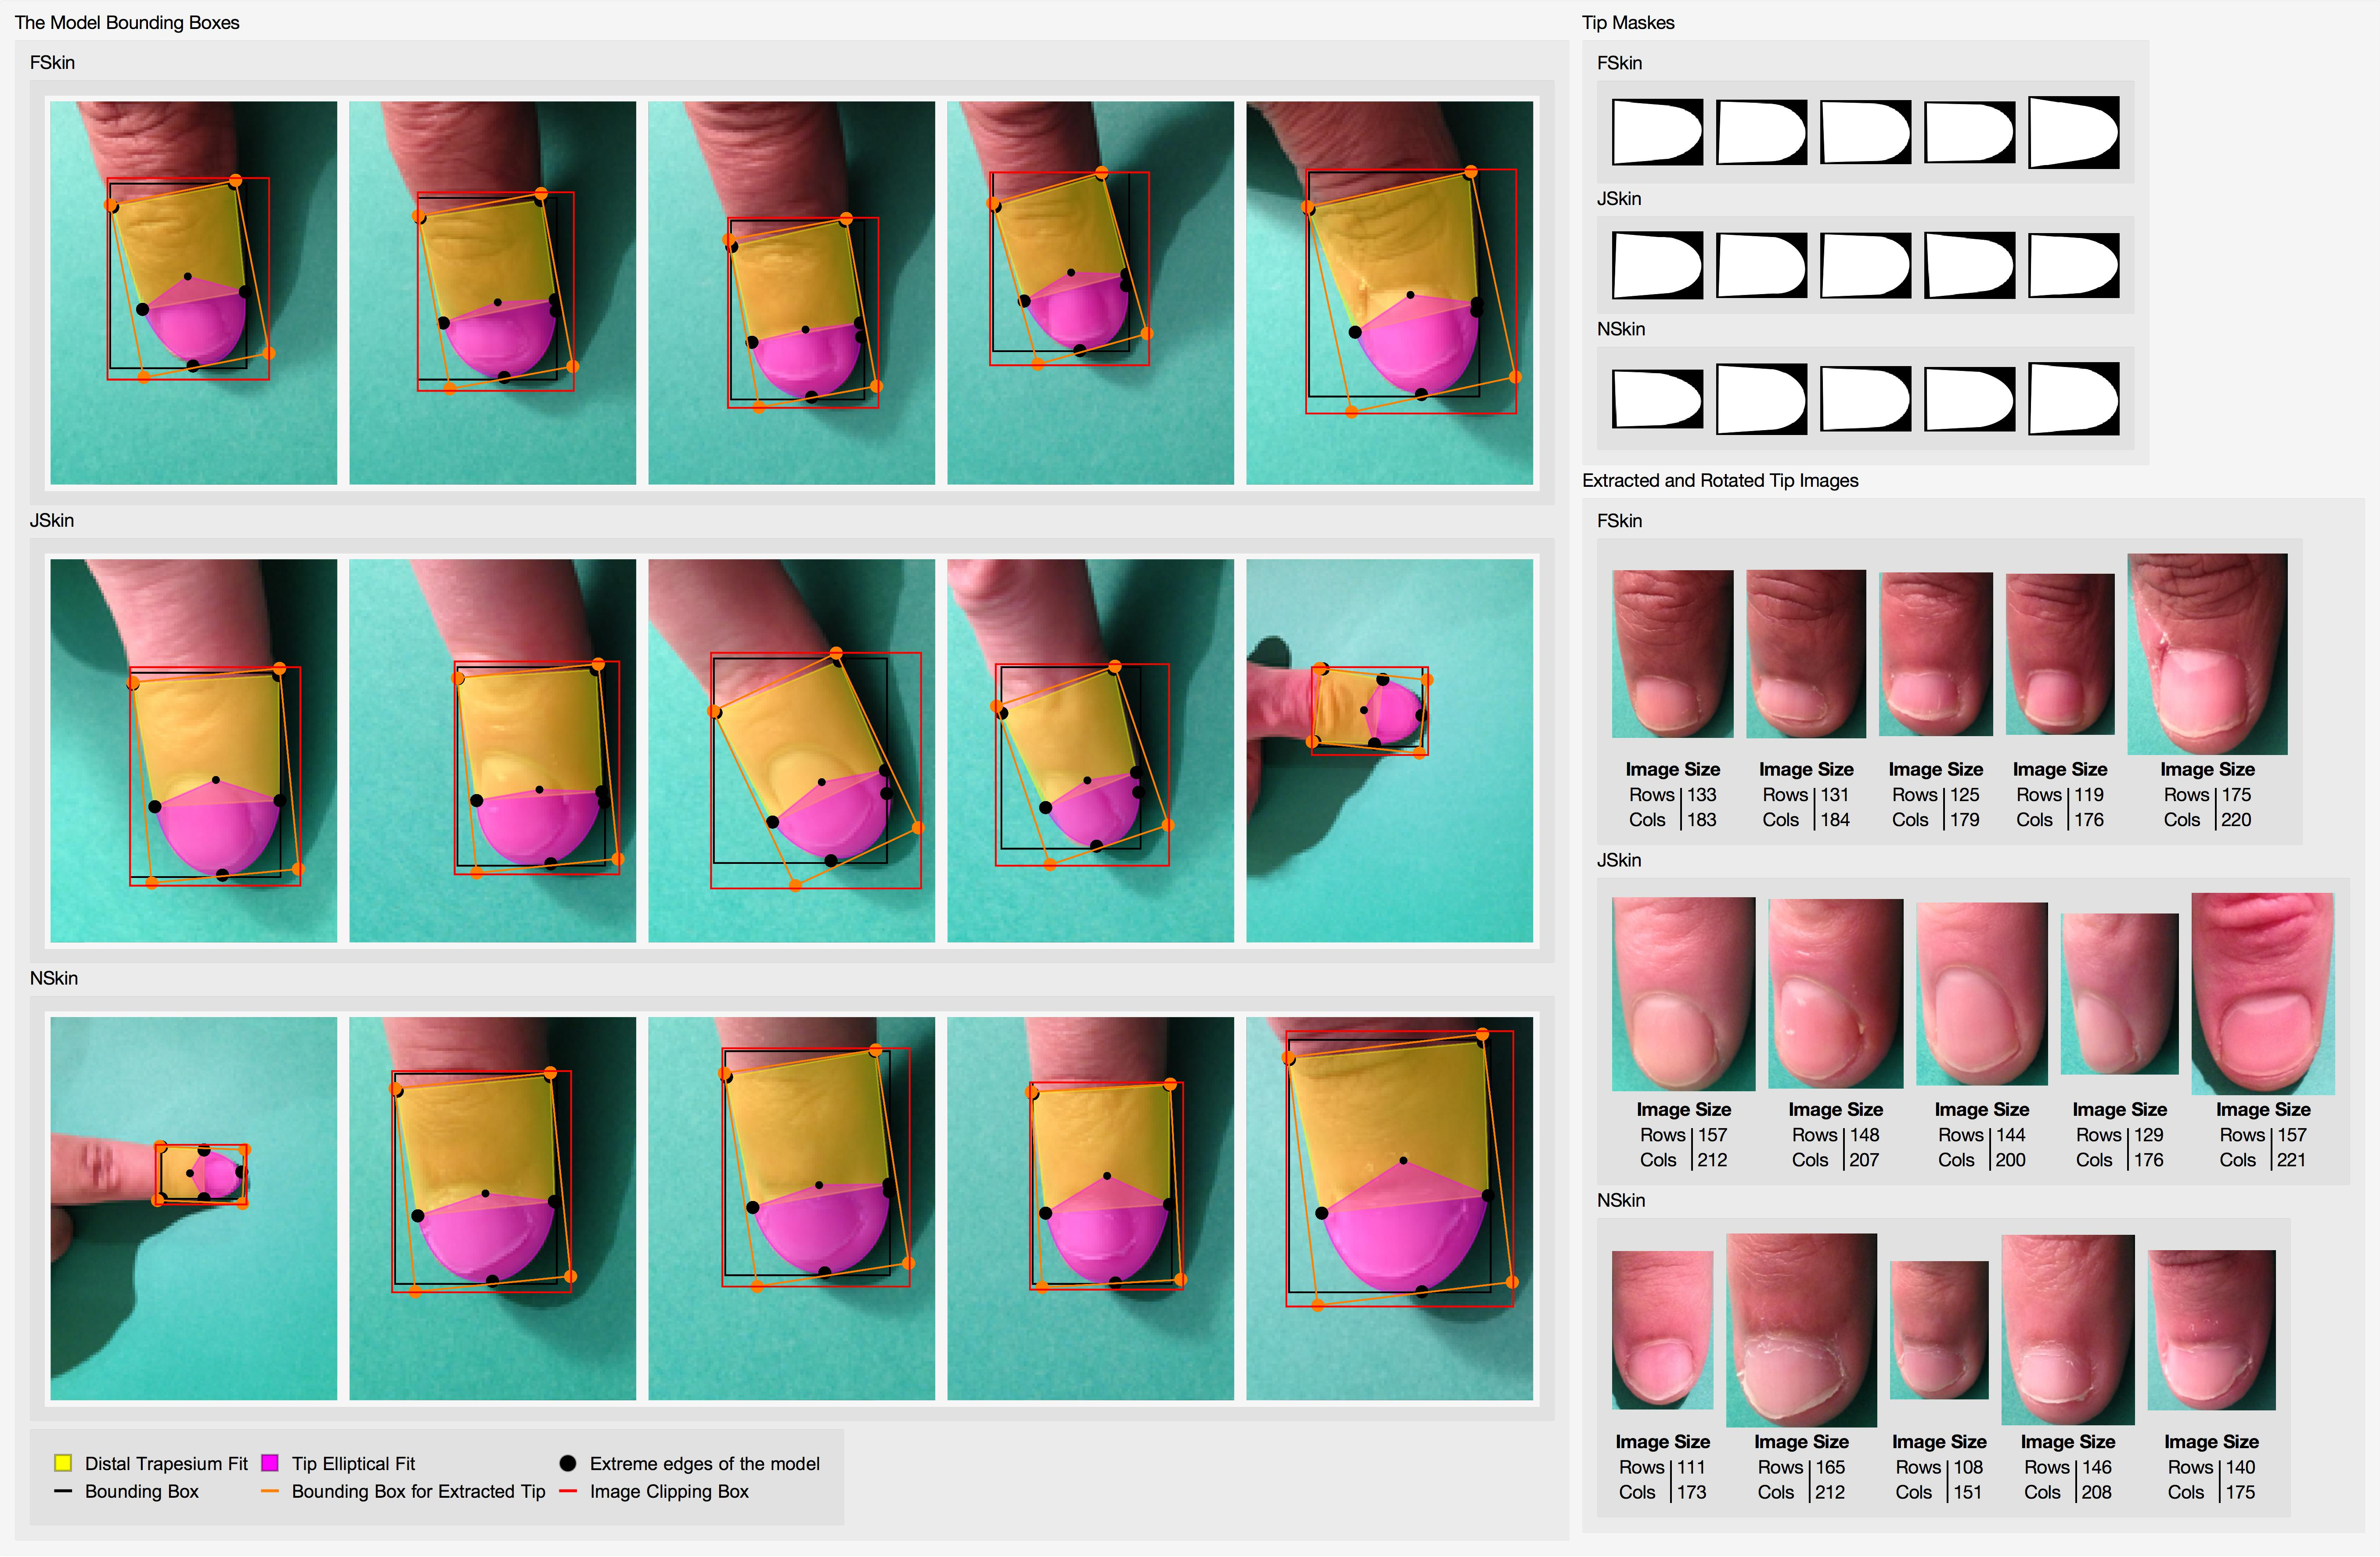
\includegraphics[width=0.95\textwidth]{Chapter4/Figs/Model_Overlayed_Boundary_with_Tips.jpg}
    \caption{The models and model boundaries overlayed on the source images. With tip masks and extracted tip images.}\label{fig:ModelOverlayedBoundaryWithTips}
\end{sidewaysfigure}


\clearpage
\section{Dynamic Tracking}\label{sec:DynamicTracking}
The main purpose of the dynamic tracking algorithm is to categorize the motion of the digit in the frame as "rapid motion," "smooth motion," and "in contact with a surface."

\begin{itemize}
\item \textbf{Rapid motion} --- When the digit is being moved into the frame, or is moving rapidly across the frame, or when the camera is being put into position, it is pointless to attempt to detect a fingertip as this information will quickly become irrelevant. Standard motion detection library routines can be used here on the unaltered video feed. When these algorithms detect motion above a certain threshold, the algorithm does nothing and waits for the motion detected to fall below this threshold.
\item \textbf{Smooth motion} --- Smooth motion is when the digit is being moved in a controlled manner within the frame. When the digit is moving in such a way, it is reasonable to assume that a finger press is imminent. The algorithm takes a frame in the small scale space and processes it into a pixel-categorized image as in Section \ref{sec:QuaternaryPixelClassification}. The frame orientation and digit tip selection are found as in Sections \ref{sec:FindingTheFrameOrientation} and \ref{sec:FindingTheEndOfTheFingerShape}, and then a Filament fill of only the tip is performed similar to Sections \ref{sec:FilamentFill} and \ref{sec:FilamentFillTheFinger}, but now with the Filament fill path being shortened to the length of the distal section in the model. The position and orientation for the model are obtained using the Force Analogue Shape Detection algorithm outlined below, in Section \ref{sec:ForceAnalogue}. The algorithm continues tracking until the change in the position of the tip between successive frames falls below a threshold, at which point the algorithm decides that the digit is likely in contact with a surface, and control passes to the "in contact with a surface" part of the algorithm.
\item \textbf{In contact with a surface (ICWaS)} --- When the tip of the digit is relatively immobile, the digit is likely in contact with a surface; we now want to observe the blood flow. The frame is now captured in the medium space, and is cropped to the edges of the model in its current position and orientation. The cropped image is put into the skin color-space, and a gradient filter is applied to the grayscale channel. If this is the first iteration, this gradient-filtered image is stored; if it is a subsequent iteration, this gradient filter is compared with the first and an alignment transform is found between the current frame and the first frame. To improve the accuracy and avoid the algorithm being distracted by movements at the edge of the digit, the gradient-filtered images are masked with the model, which removes edge-related gradient features, focusing the algorithm on the nail, which is stable during a finger press. The transform is applied to the two chromatic channels, which aligns the images, and the difference is found between successive frames; this gives us the blood flow. 
\end{itemize}

\subsection{Rapid Motion Tracking}\label{sec:RapidMotionTracking}
Before any fingertip tracking is performed, the algorithm checks to see if the digit is still in motion. This is done by first taking the difference between subsequent grayscaled frames from the raw video feed using OpenCV's `absdiff' method. To account for changes in lighting and contrast, a binary threshold is applied to the frames, after which an erosion operation (the `erode' method) is performed to further reduce artifacts and false positives. If the number of changes in the image is above a given threshold, then the digit is considered to be in rapid motion.


\subsection{Smooth Motion Tracking}\label{sec:SmoothMotionTracking}

The find-tip algorithm (Section \ref{sec:FindingTheEndOfTheFingerShape}) gives us a path which we know lies on a digit. This path, however, is not necessarily particularly well-aligned with the axis of the digit. For this reason, we don't ask for a shortened path from the tip to $1 \frac{1}{2}$ distal widths along that path; such a path might actually end closer to the tip than desired, as the path isn't necessarily along the axis. To account for this, we ask for two distal widths from the tip. 

The next problem to be addressed results from the operation of the Filament fill method; because the digit isn't necessarily presented perpendicularly to the frame edge and the Filament fill algorithm finds points perpendicular to the frame edge, we adjust by half the gradient of the path, similarly to the method used in the fingertip model algorithm illustrated in Figure \ref{fig:ModelingFingertip}. So, Filament fill is run along the find-tip path from the tip to a distance of $(2+\left\lvert\frac{1}{2}\delta path\right\lvert)w$ from the tip. This gives us three sets of points: the top, middle and bottom edges, which definitely include points relating to the tip of the digit.

Now we refine these points; because we know the orientation of the frame, we can determine which points correspond to the top edge of the digit, and which points correspond to the bottom. We now put them into standard orientation as in steps a and b in Figure \ref{fig:ModelingFingertip}. 

We now need to find points on the model which would ideally correspond with the points found by Filament fill in the image. First, we need to obtain a reasonably good measure of the orientation of the digit; given that we have midline points on the digit which reasonably correspond to the distal segment, a linear fit to the middle $\frac{2}{3}$ of these points provides a good measure of the orientation with little computational cost. Rather than reorientating the image points to a neutral coordinates, we rotate the model to correspond with the image coordinates. This is easily achieved as the model is centered on the ellipse, and so involves a rotation of the four points of the trapezian and adding the rotation to the ellipse's orientation.

In the model's new orientation, we find the furthest point on the model in the $x$ axis. (It should be noted that this is not necessarily what we would refer to as the "tip" of the digit.) We assume that this point on the model corresponds to the first point in the midline set of points; the Filament fill follows the path from the tip back to the frame edge, so the first point in the midline should be the tip. So, we create a set of $x$ axis coordinates where the first midline point corresponds with the furthest point on the model in the $x$ axis. We do this because the Filament fill divides up the shape vertically in a relatively regular fashion, so we are dividing up the model in the way that we would expect Filament fill to if the model were an image. This allows us to put points on the model and points in the image into a $1:1$ correspondence. So although the fingertip model is a relatively arbitrary geometric shape, the regularity of the Filament fill method allows us to use a force analogue shape detection algorithm as outlined previously (Section \ref{sec:ForceAnalogue}).

\begin{figure}[h!]
  \centering
    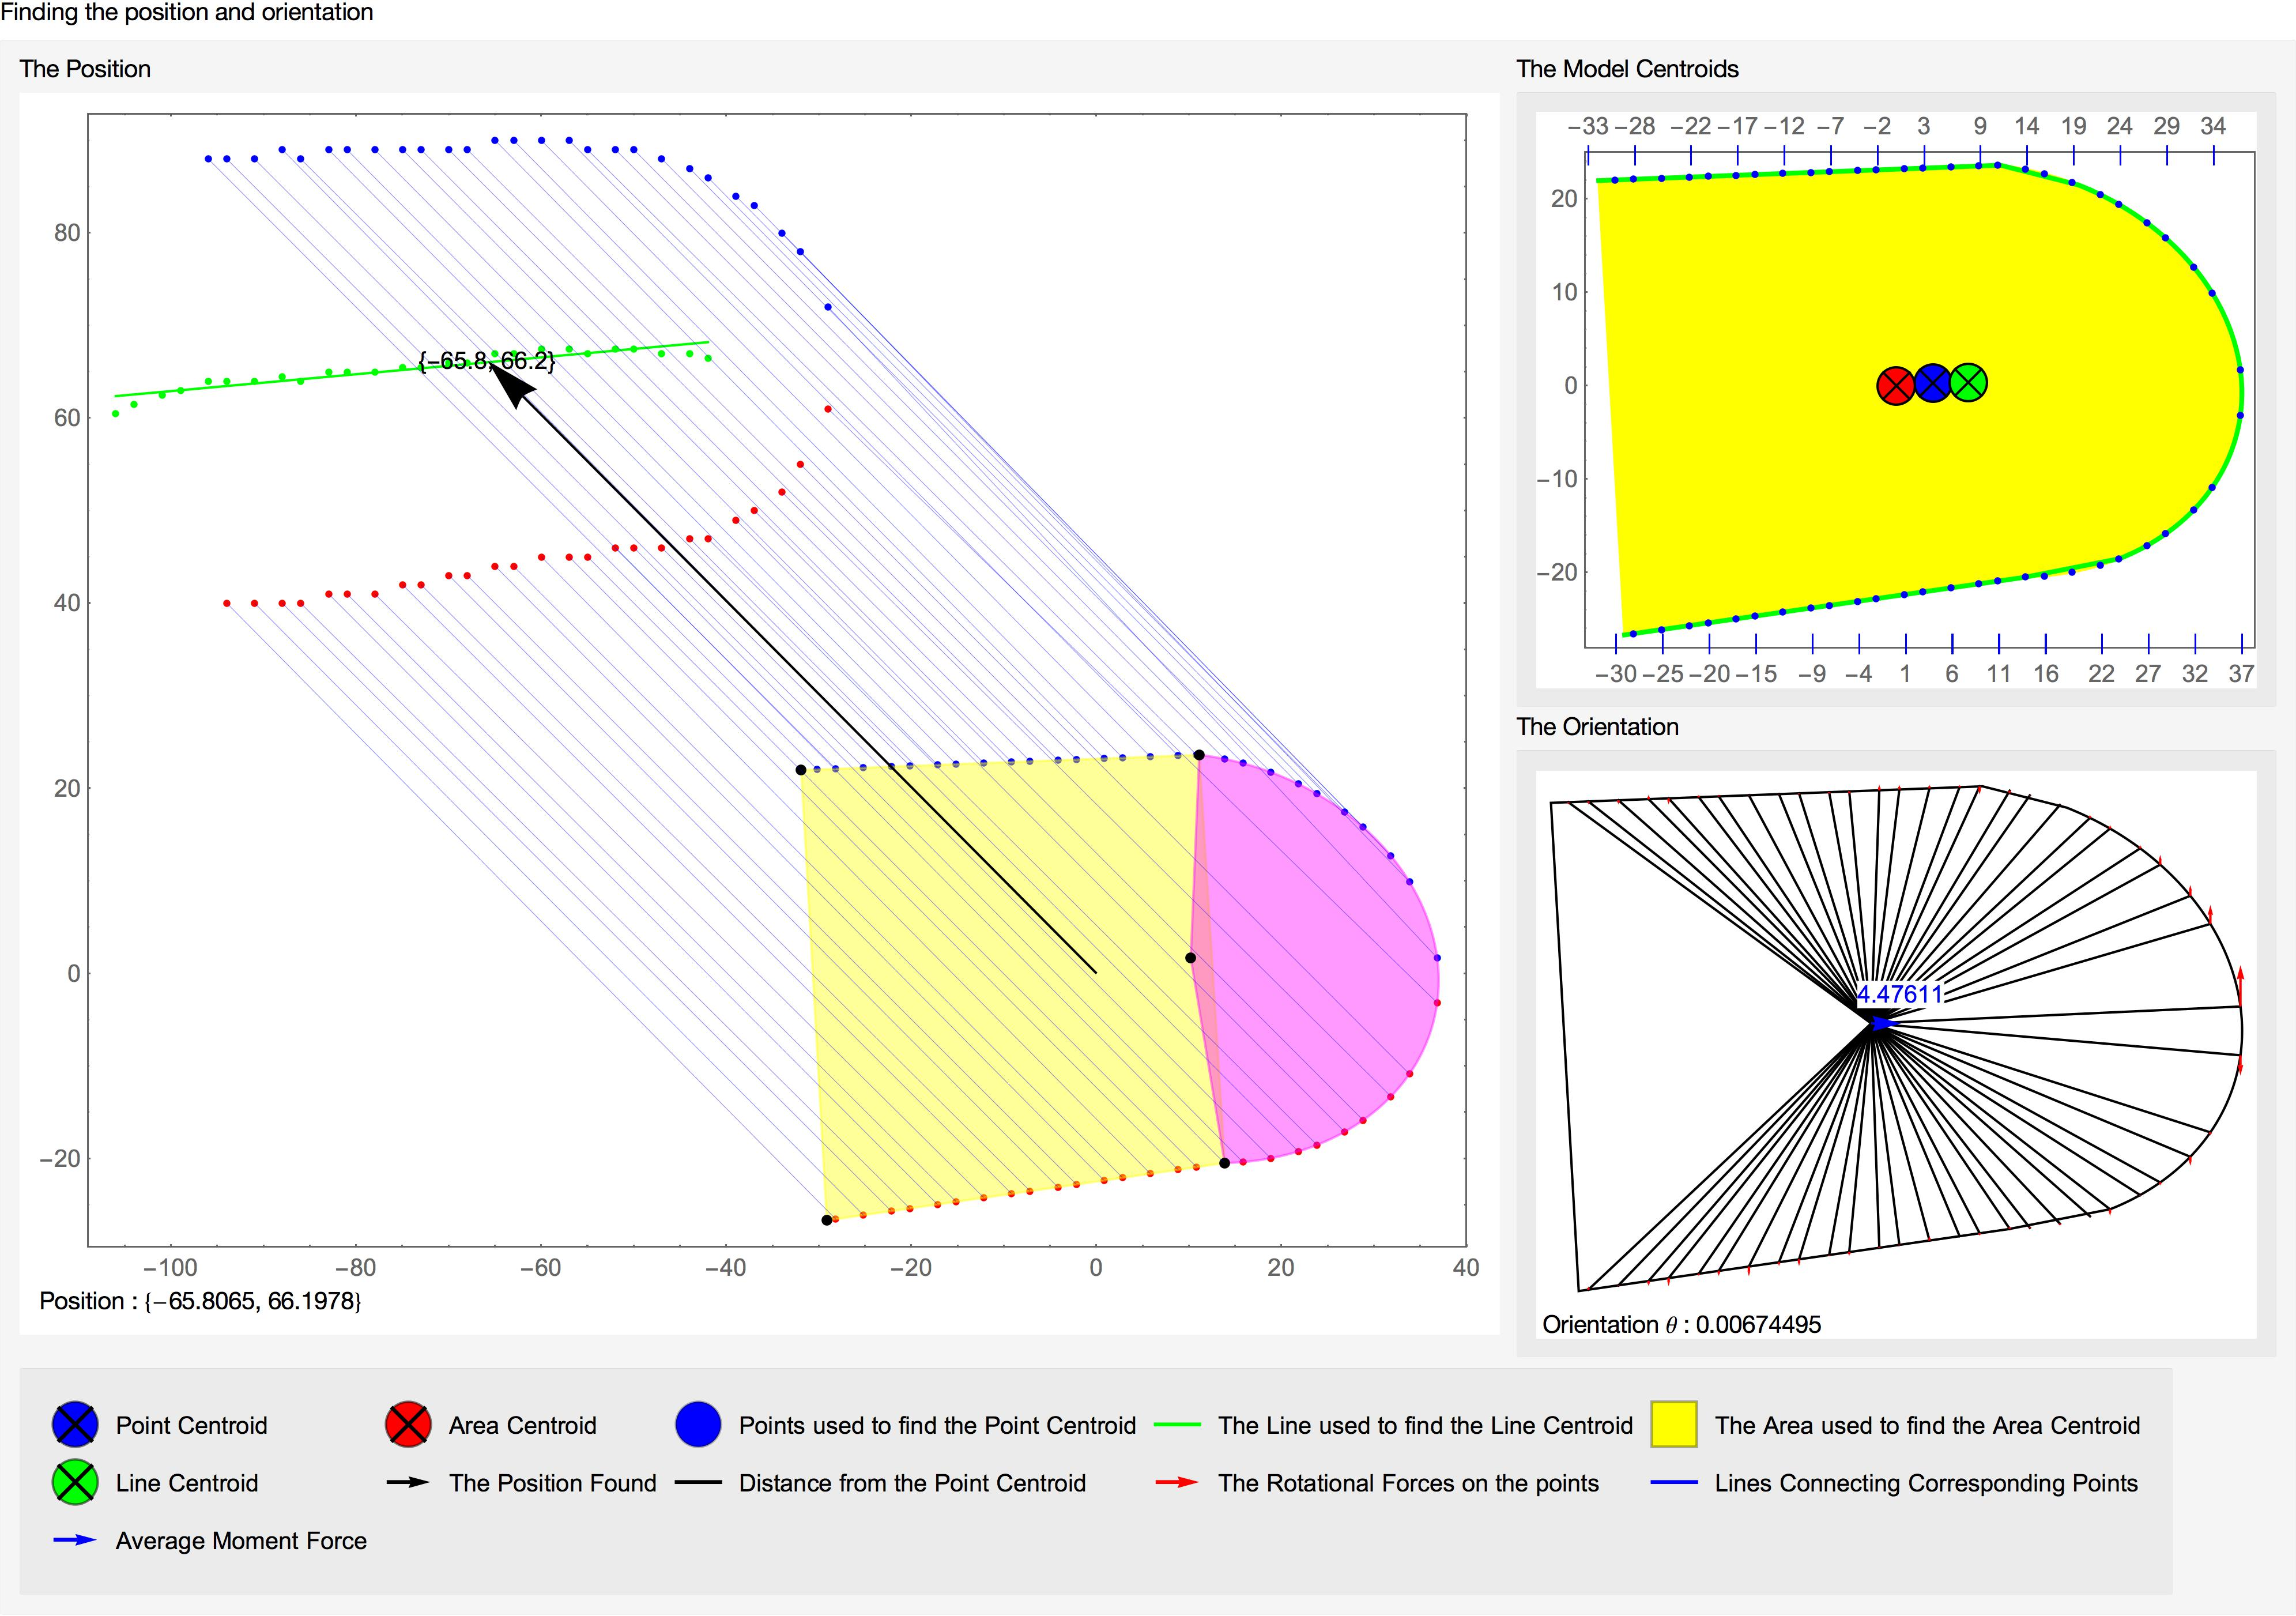
\includegraphics[width=0.95\textwidth]{Chapter4/Figs/Model_Centroids_With_Pos_Orientation.jpg}
    \caption{Finding the Position and Orientation of the Tip. A side-effect of the pre-alignment of the model means that, almost always,  the change in the orientation from the force analogue shape detection algorithm is negligible. }\label{fig:PositionAndOrientation}
\end{figure}

A side-effect of the pre-alignment of the model means that --- almost always --- the change in the orientation from the force analogue shape detection algorithm is negligible.

The distribution of points around the perimeter of the model is dependant on the orientation of the digit in the image. This means that the point centroid is not constant, and so a shape-based area centroid is used in the modeling stage (Figure \ref{fig:PositionAndOrientation}). 

\begin{figure}[h!]
  \centering
    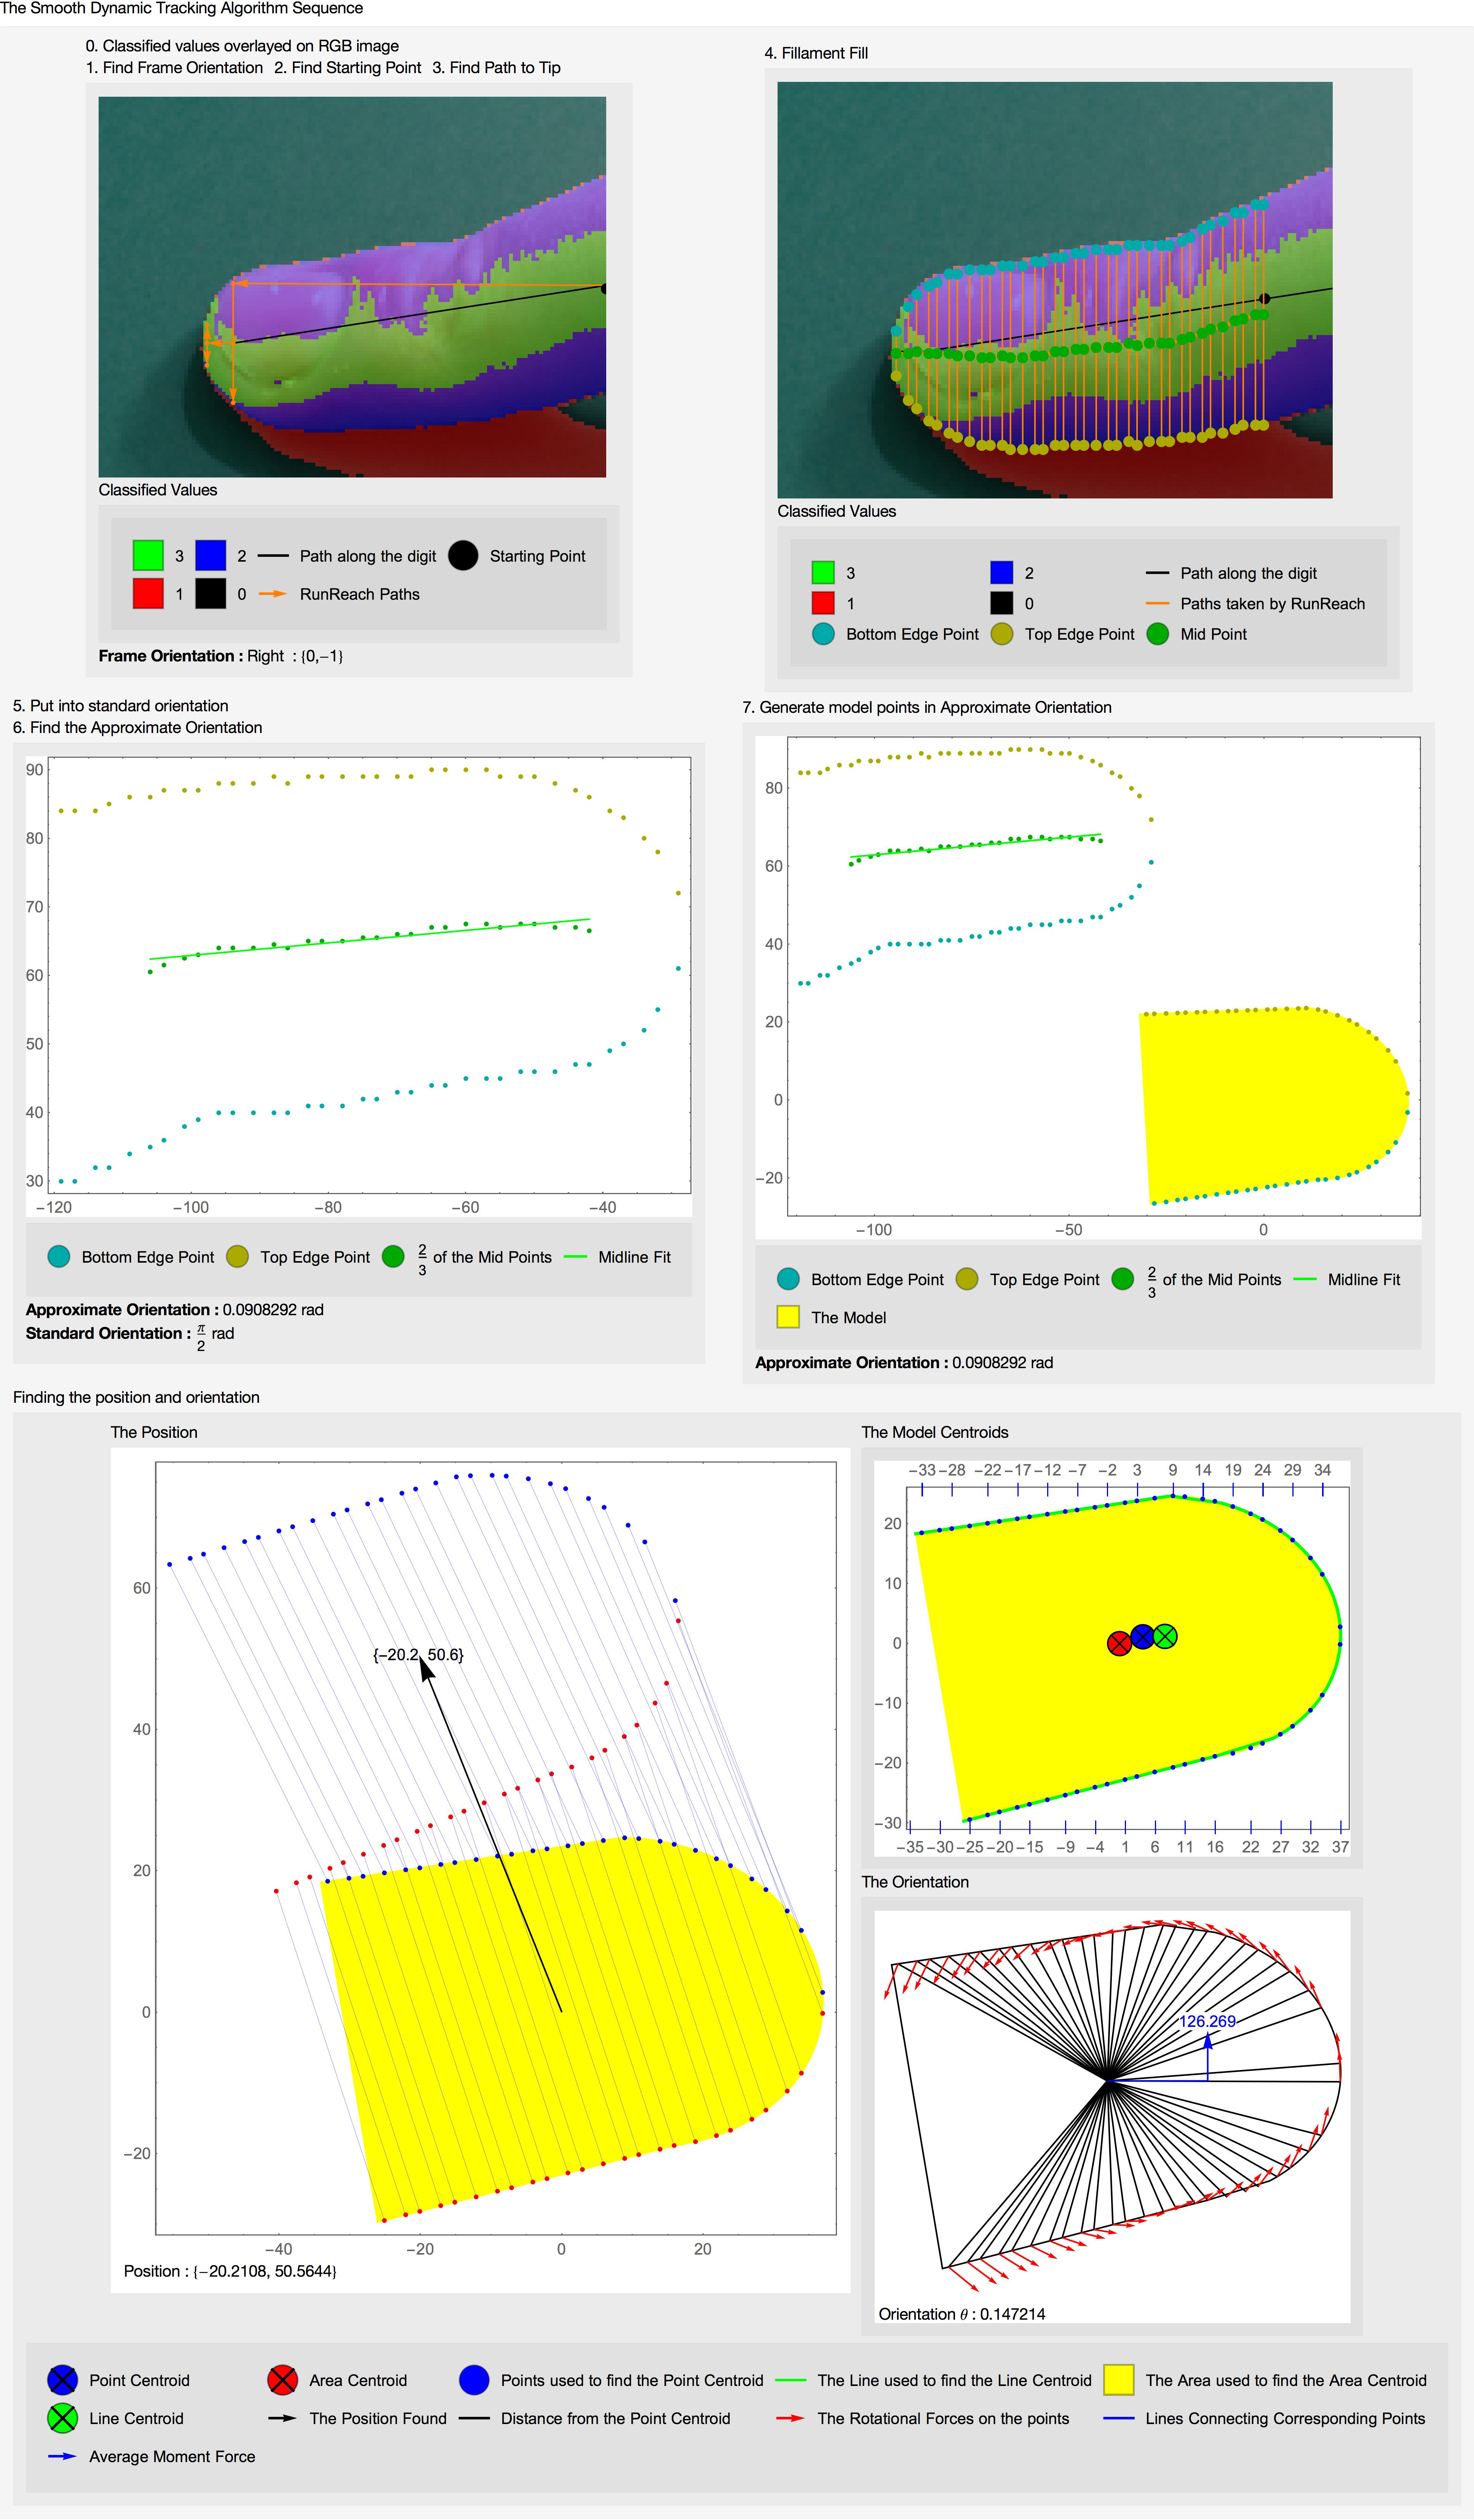
\includegraphics[width=0.85\textwidth]{Chapter4/Figs/Smooth_Dynamic_Sequence.jpg}
    \caption{Smooth Dynamic Sequence}\label{fig:SmoothDynamicSequence}
\end{figure}


In practice, the algorithm first finds the rough orientation of the digit in the image and rotates the model accordingly. The model is re-centered on the point centroid for the current orientation before the FASDM method is used. 

In addition to the FASDM method, the algorithm also finds the mean of the length of the vectors between the rotated and translated model points and the points on the image. To be clear, this distance is signed according to which point is further away from the model center. This allows the model to be scaled. The upshot of this is that the code correctly follows a digit even as the digit moves closer or further away from the camera. (Fingers do not normally change shape.)
\clearpage
\subsection{ICWaS Method}\label{sec:ICWaS}
The ICWaS method performs three main tasks: cropping the midscale image around the tip; providing a multiplicative mask which highlights blood flow in the tip; and aligning successive frames in-order to find the pixel color differences in the skin color-space. Combining these three tasks allows the blood flow to be shown.

\subsubsection{ICWaS Setup}\label{sec:ICWaSSetup}
From the Smooth Movement Tracking (Section \ref{sec:SmoothMotionTracking}), we have a model position and orientation in the small scale space. We wish to track the blood flow using the medium scale image, so first we must put the model in the medium scale space. This is as simple as multiplying the coordinates by a scaling factor as shown in Section \ref{sec:ScaleSpace}.

Now we want to find the extreme top, bottom, left and right edges of the model in order to crop the midscale image appropriately. The model is comprised of a quadrilateral and an ellipse. To find the extreme edges of the quadrilateral, the algorithm just finds the minimum and maximum values of the coordinates of its vertices. The ellipse's extreme edges can be found using

\begin{minipage}{0.7\textwidth}
\begin{align*}
\begin{array}{ll}
e_1= \Bigg( x_0+\frac{(a-b) (a+b) }{A} \sin \left( \theta \right) & , y_0+A \cos \left( \theta \right) \Bigg)\\
e_2=  \Bigg( x_0-\frac{(a-b) (a+b)}{A} \sin \left( \theta \right) & , y_0-A \cos \left( \theta \right) \Bigg)\\
e_3=  \Bigg( x_0-B \cos \left( \theta \right)  & , y_0-\frac{(a-b) (a+b) }{B} \sin \left( \theta \right) \Bigg)\\
e_4=  \Bigg( x_0+B \cos \left( \theta \right)  & , y_0+\frac{(a-b) (a+b) }{B} \sin \left( \theta \right) \Bigg)\\
\end{array} \\
 \text{where}\quad 
\begin{array}{c}
A=\sqrt{a^2 \tan ^2(\theta )+b^2} \\
B=\sqrt{a^2+b^2 \tan ^2(\theta )} \\
-\frac{\Pi}{2}< \theta < \frac{\Pi}{2}
\end{array}
\end{align*}
\end{minipage}%%%%%%%%%%%%%%%%
\begin{minipage}{0.3\textwidth}
 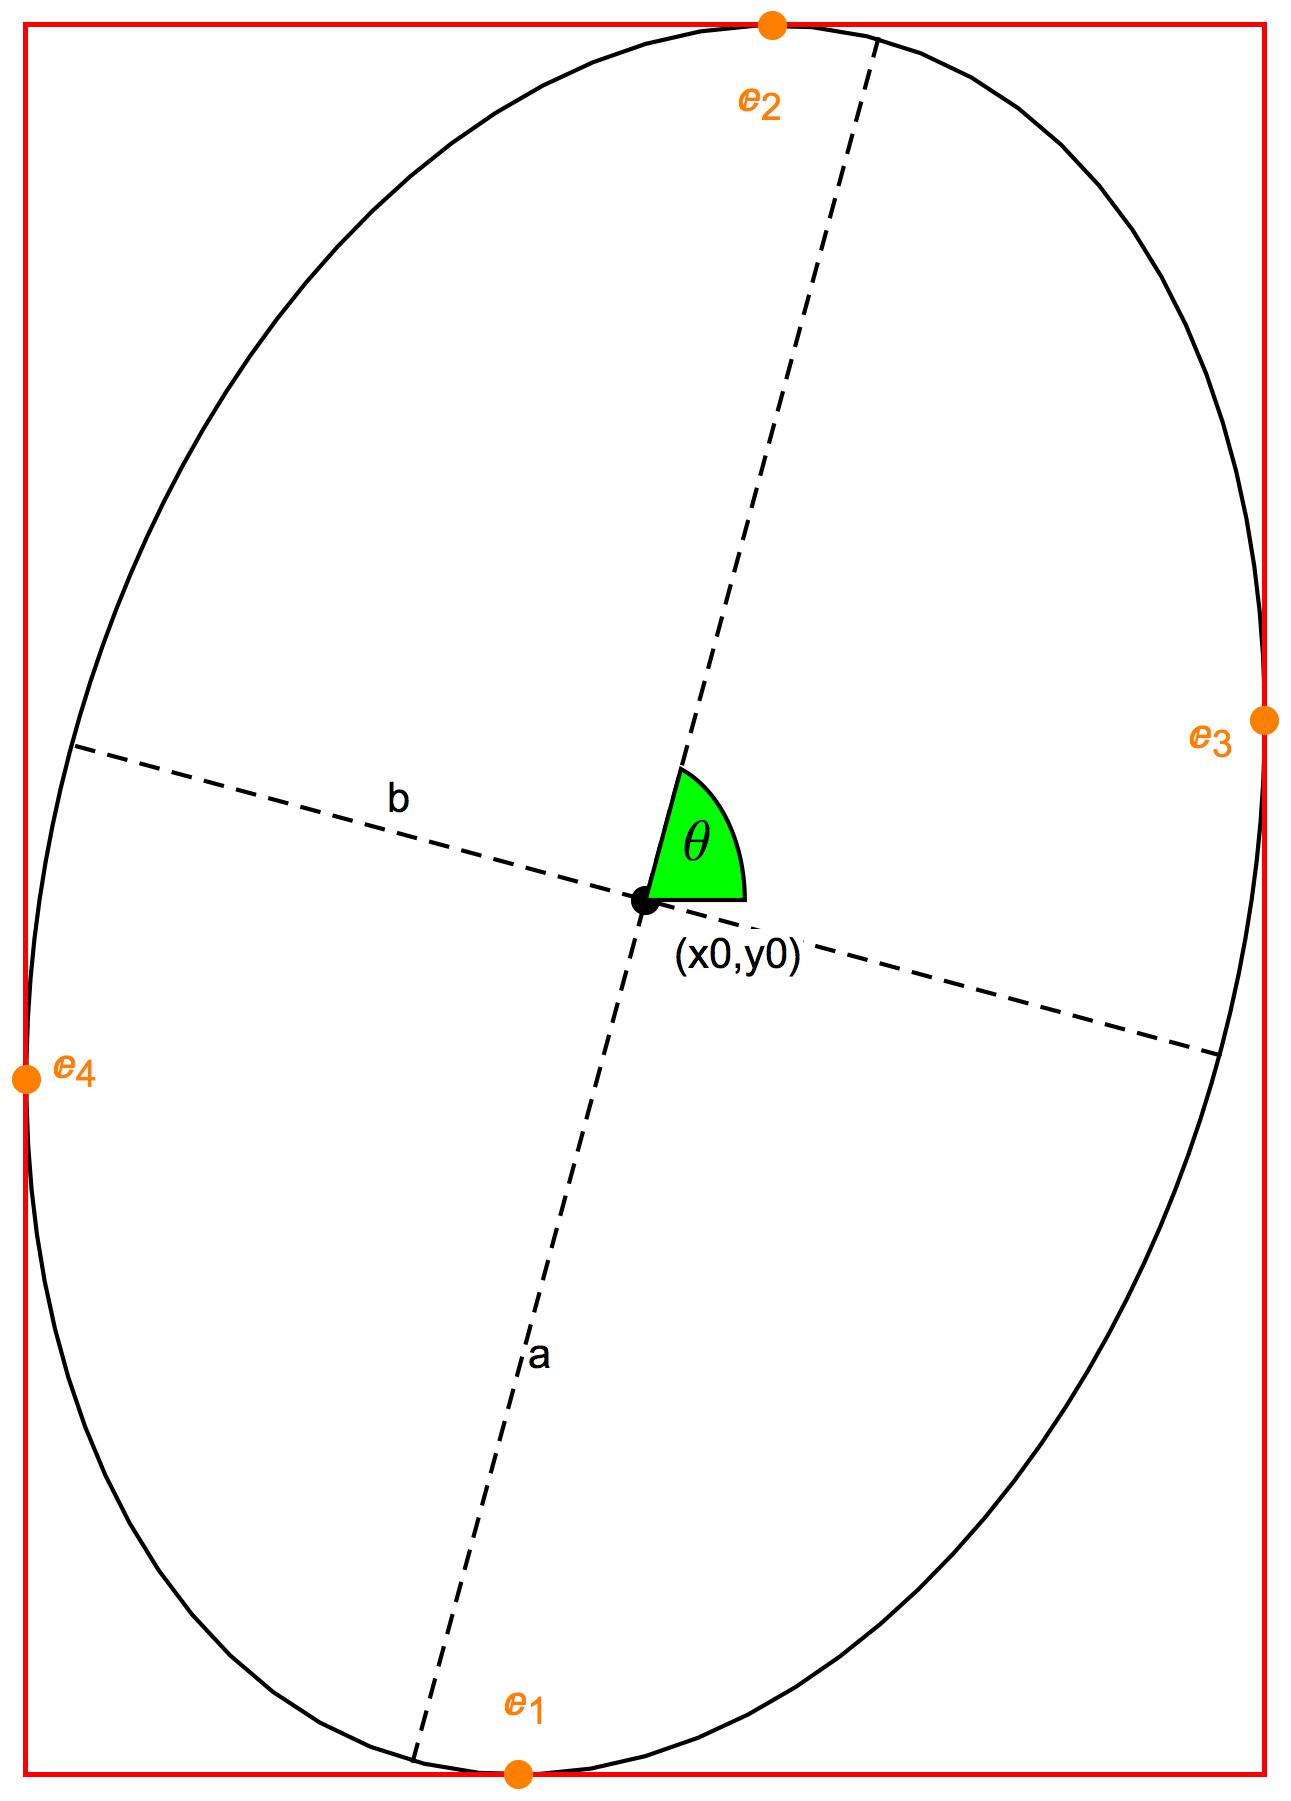
\includegraphics[width=\textwidth]{Chapter4/Figs/Elliptical_Bounds.jpg}
\end{minipage}


However, we only want to include extreme points which lie on the curve which models the tip. The curve which models the tip is the part of the ellipse which falls between the two points on the quadrilateral closest to the tip; we can check if the extreme edges of the ellipse are on this part of the curve by checking that they lie at an angular position between the angles at which the tipmost quadrilateral points lie.

Now we have the extreme edges of the model. These points are used to find a bounding box, which includes all the tip pixels in the small scale space. Translating these to the medium scale space, we subtract the scaling factor from the lower coordinates and add the scaling factor to the higher coordinates, ensuring that the box does not crop any pixels from the digit in the medium scale space. We now take the medium scale RGB image, crop it to the model bounding box, and then pass the extracted tip image to the skin color-space processing routines. The grayscale image is saved as a template for the template matching algorithm.

During a finger press, we expect the flesh to deform around the tip, making the edges of the digit unreliable for alignment, so we wish to construct a binary mask which tells the template matching algorithm which pixels to use for alignment. Using OpenCV's drawing routines, we render the model in the midscale tip image coordinates. This is done in a way which actually renders the model 'slightly' by four or five pixels smaller than the model proper. This effectively eliminates the edge of the digit next to the background, pushing the algorithm to rely on features which do not deform, such as the nail.

\subsubsection{Blood Flow}\label{sec:BloodFlow}

\begin{figure}[h!]
  \centering
    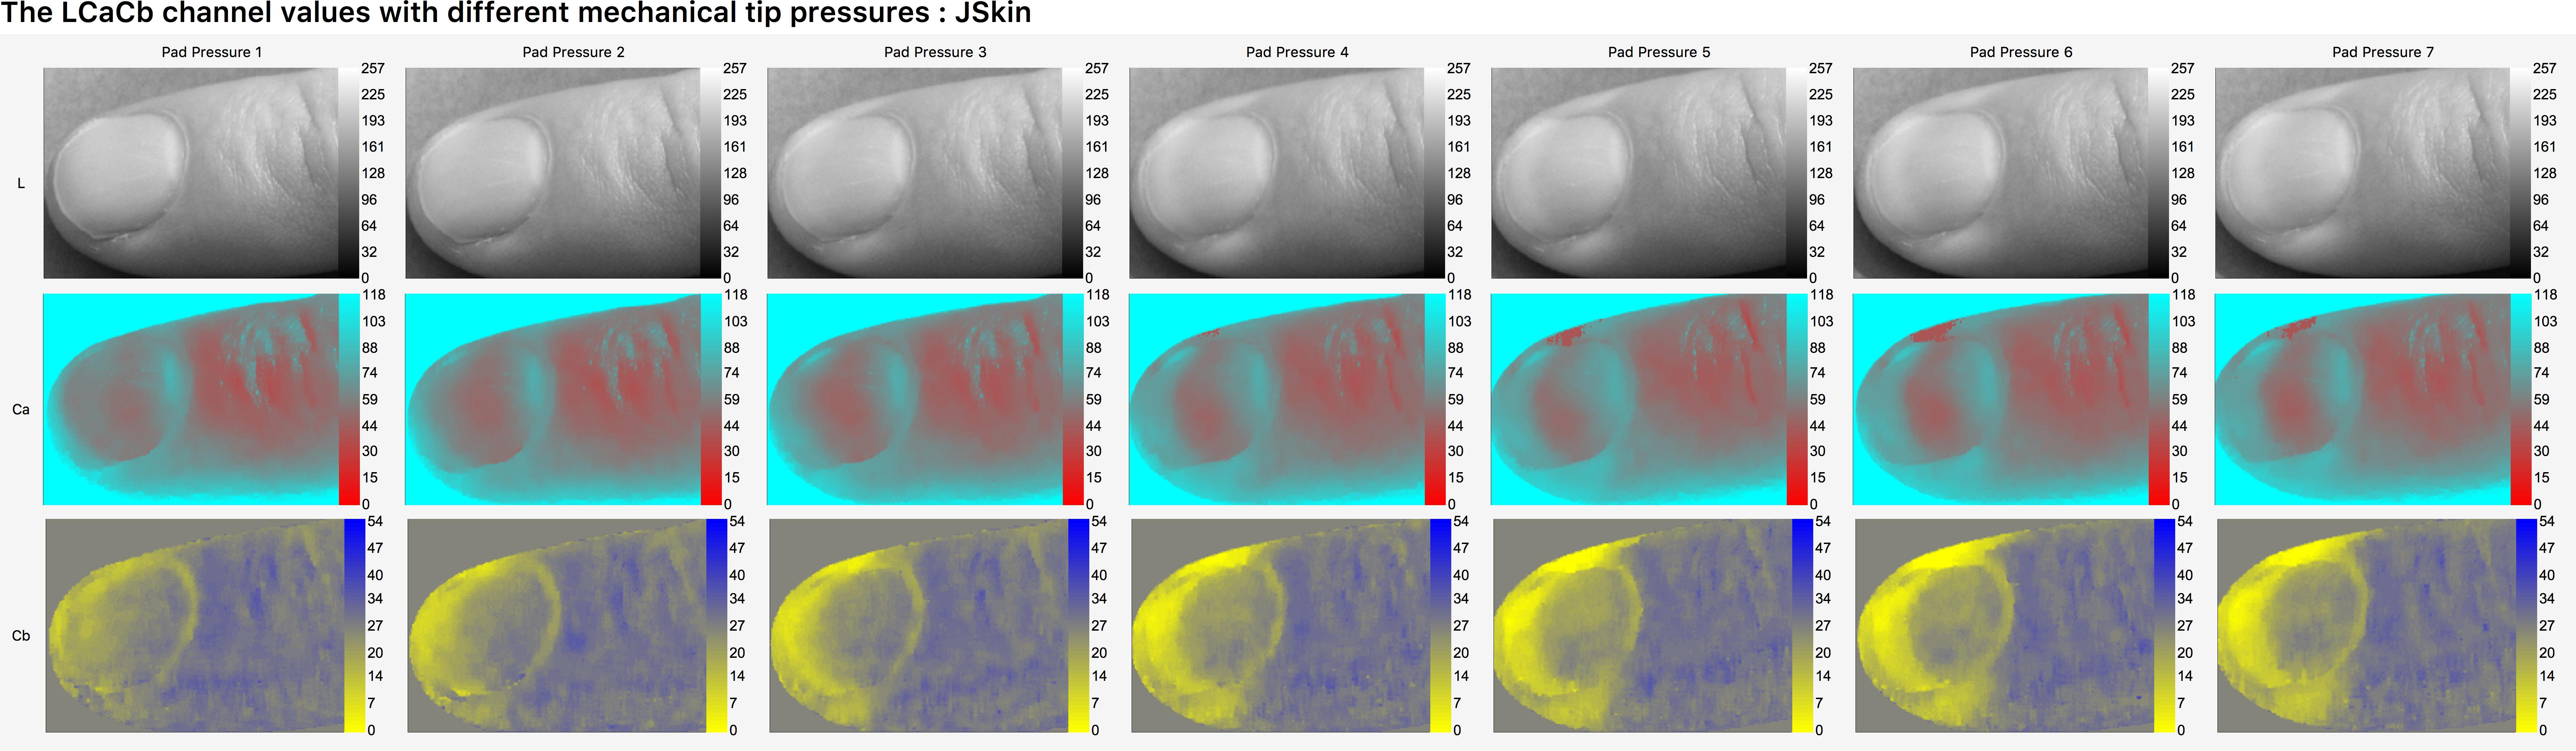
\includegraphics[width=1.00\textwidth]{Chapter4/Figs/Final_Fig_Channels_JSkin.jpg}
%    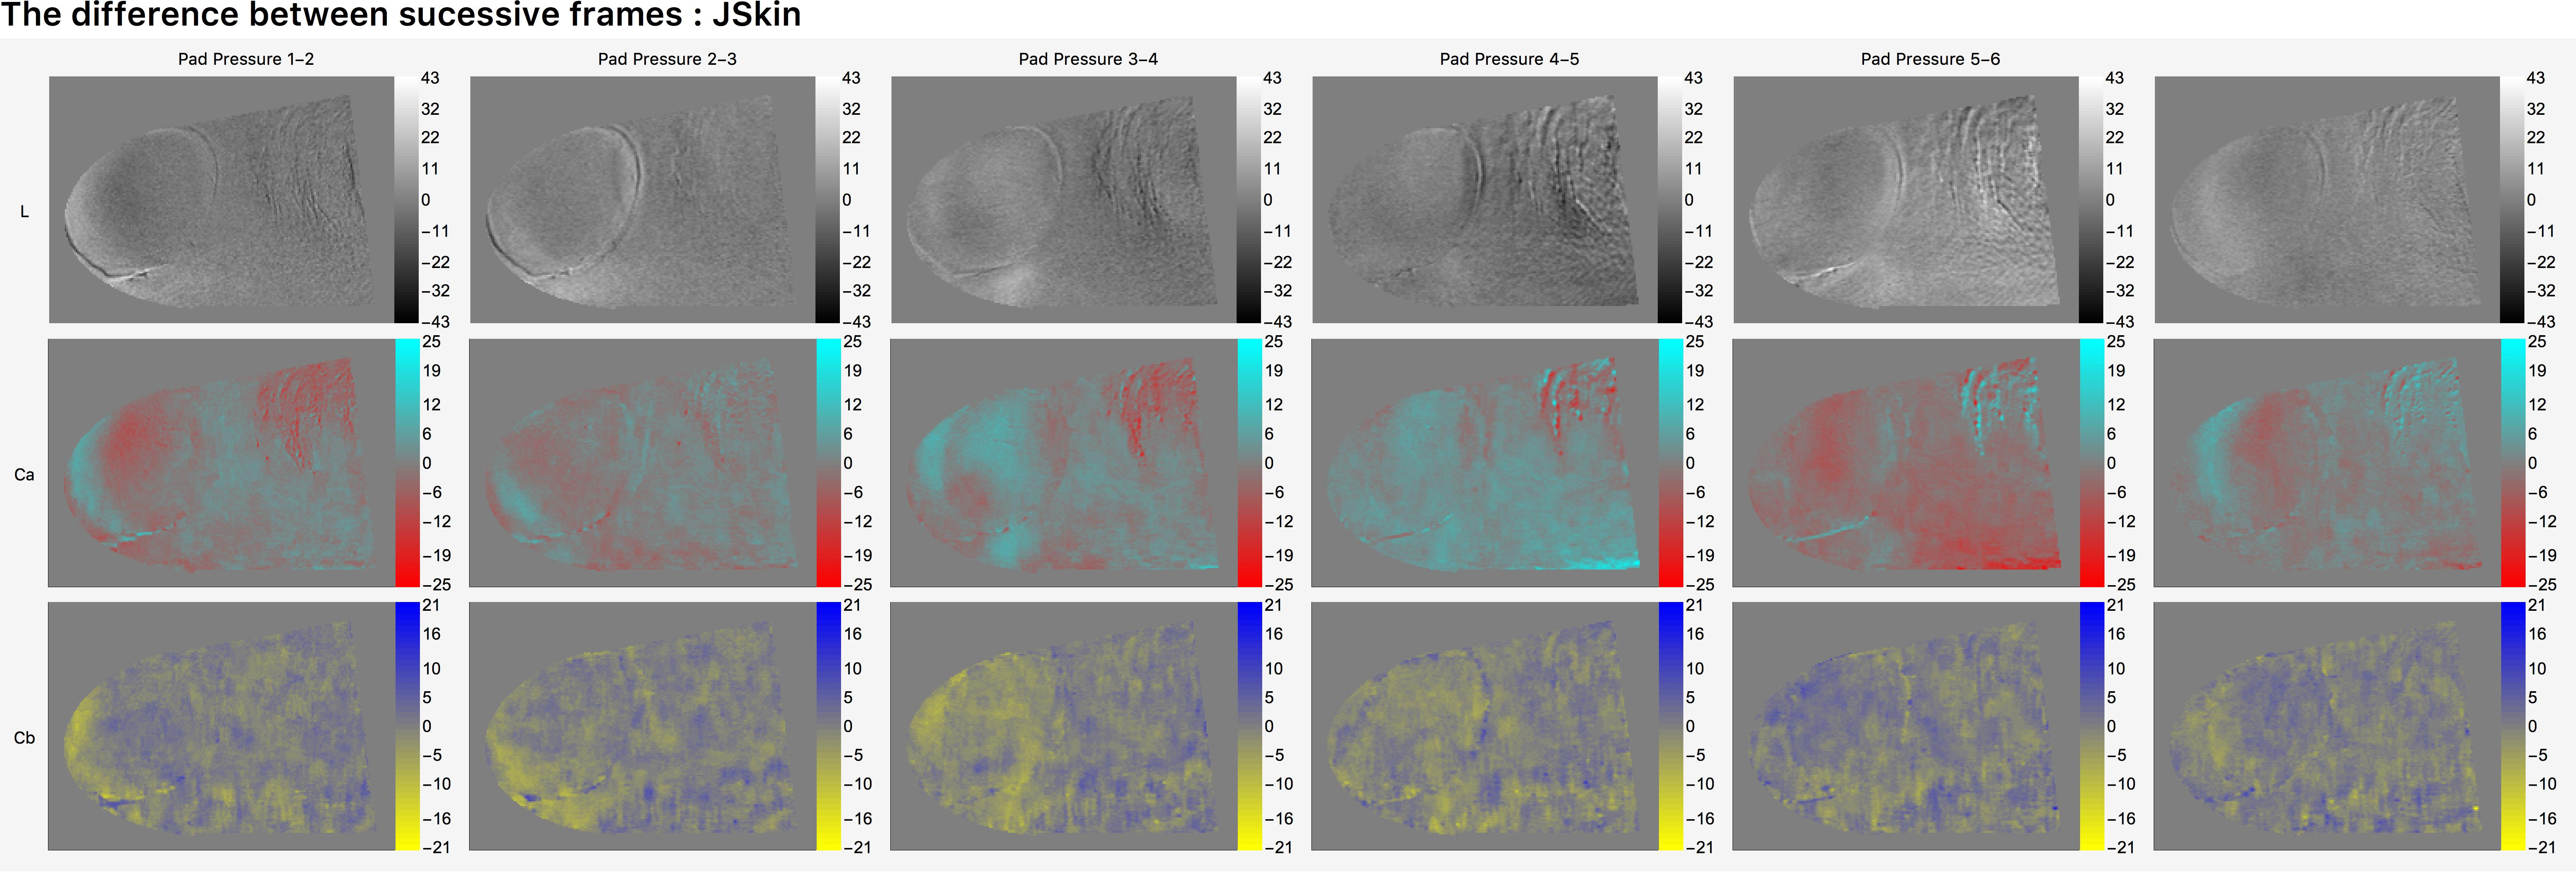
\includegraphics[width=0.86\textwidth]{Chapter4/Figs/Final_Fig_Difference_JSkin.jpg}
    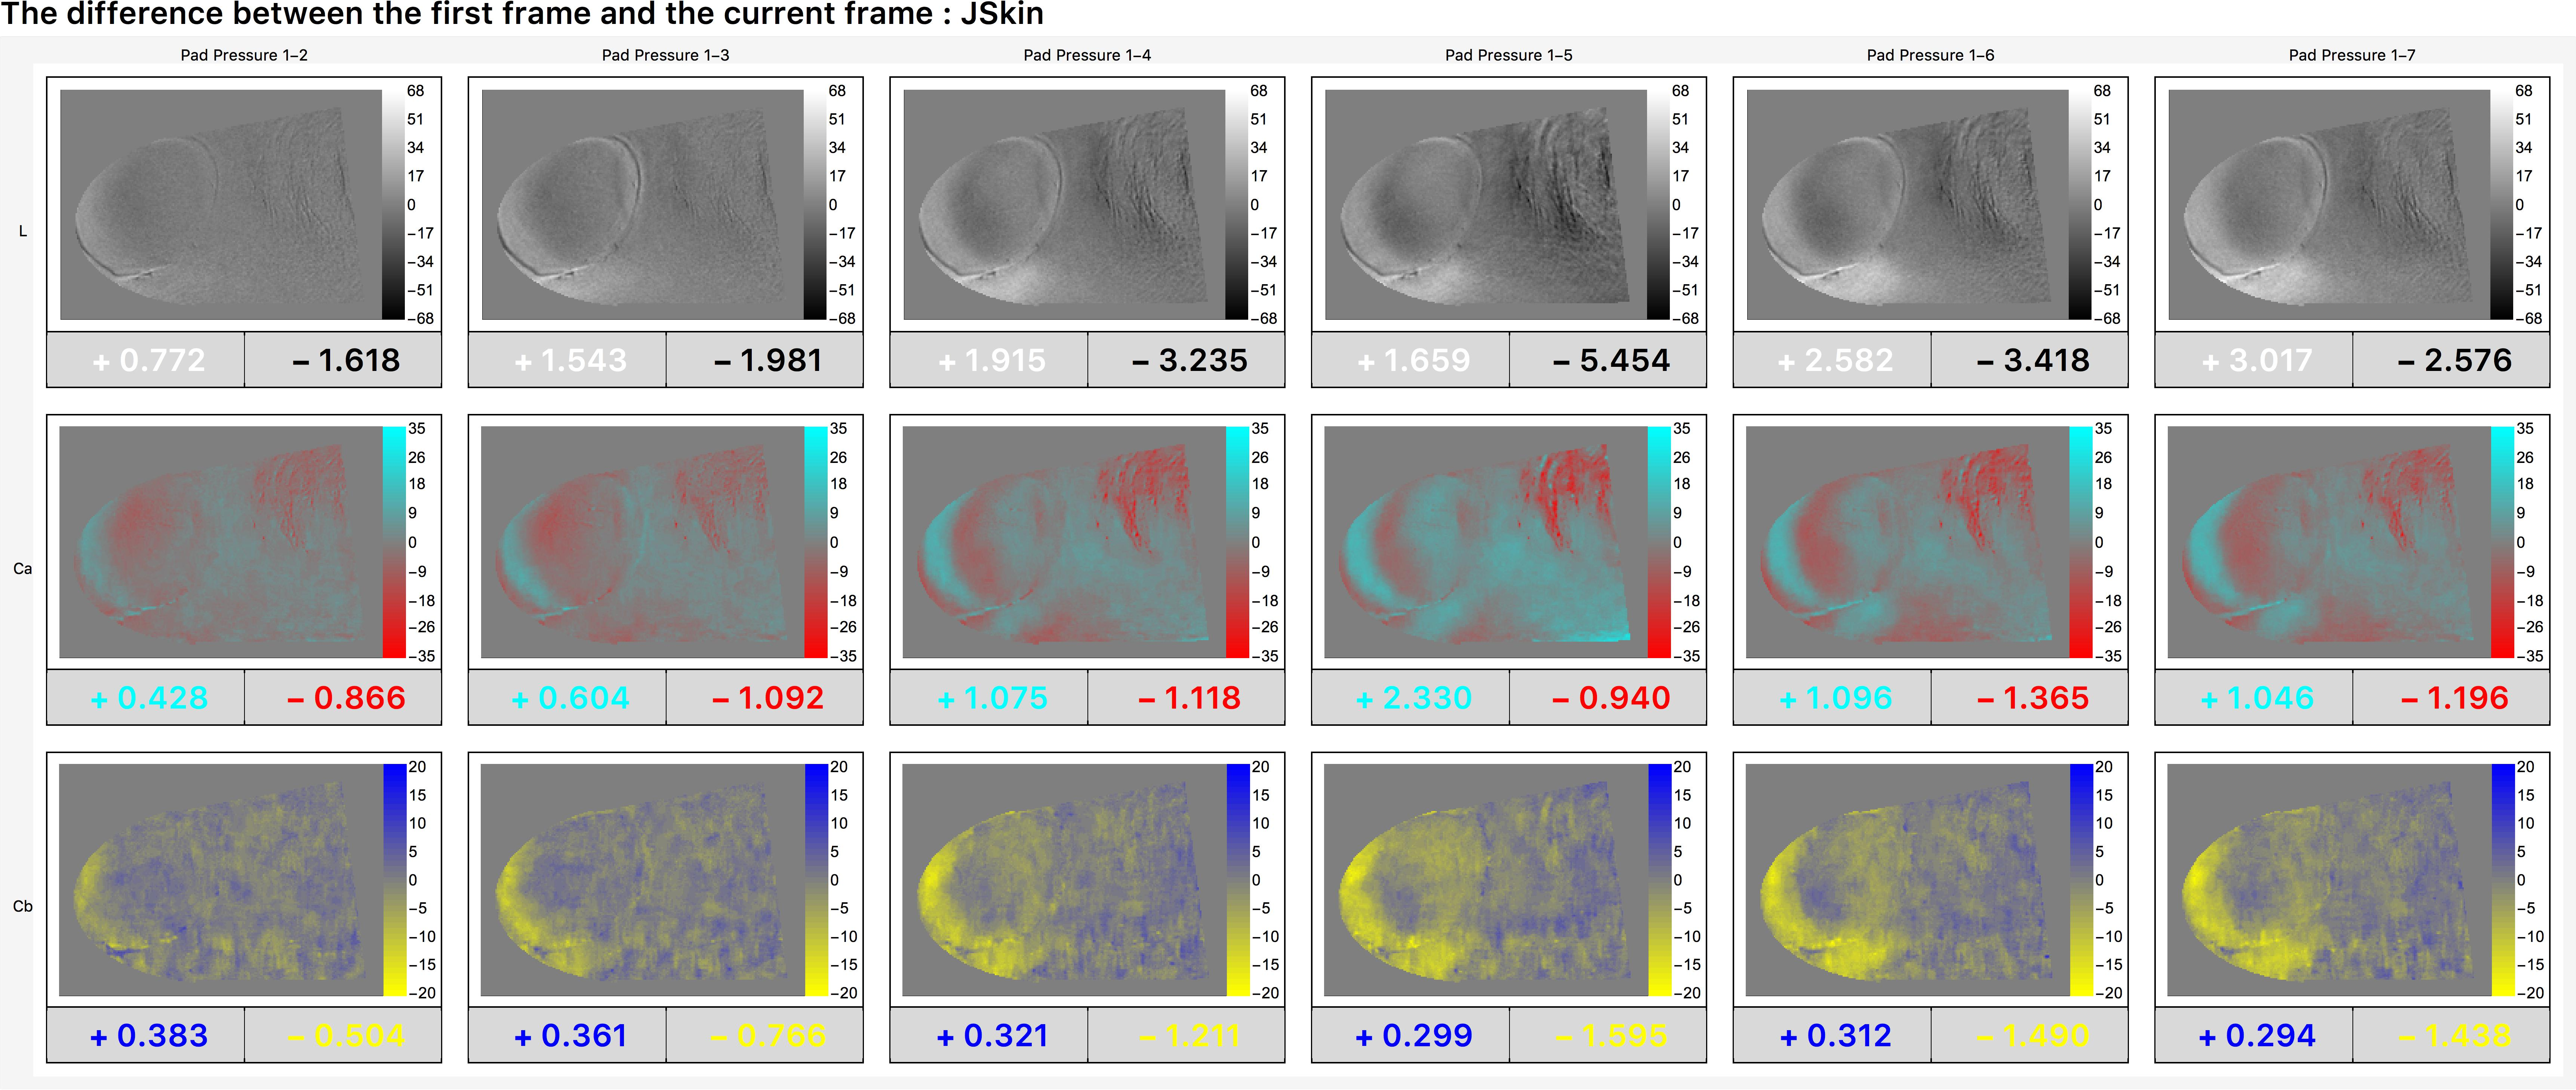
\includegraphics[width=0.86\textwidth]{Chapter4/Figs/Final_Fig_Total_Difference_JSkin.jpg}
    \includegraphics[width=1.00\textwidth]{Chapter4/Figs/Final_Fig_Misc_JSkin.jpg}
    \caption{The resulting sequence of images from the ICWaS algorithm followed by the differences. The metric is the result of summing the positive and negative changes separately and then dividing by the number of pixels. Finally, the initial image of the sequence is shown with the model outline, the slightly larger model used to set the crop frame and the slightly smaller model used for setting the mask.}\label{fig:ICWaSResultJSkin}
\end{figure}

\begin{figure}[h!]
  \centering
    \includegraphics[width=0.820\textwidth]{Chapter4/Figs/Final_Fig_Channels_FSkin.jpg}
%    \includegraphics[width=0.660\textwidth]{Chapter4/Figs/Final_Fig_Difference_FSkin.jpg}
    \includegraphics[width=0.660\textwidth]{Chapter4/Figs/Final_Fig_Total_Difference_FSkin.jpg}
    \includegraphics[width=0.820\textwidth]{Chapter4/Figs/Final_Fig_Misc_FSkin.jpg}
        \caption{The resulting sequence of images from the ICWaS algorithm followed by the differences. The metric is the result of summing the positive and negative changes separately and then dividing by the number of pixels. Finally, the initial image of the sequence is shown with the model outline, the slightly larger model used to set the crop frame and the slightly smaller model used for setting the mask.}\label{fig:ICWaSResultFSkin}
\end{figure}


\begin{figure}[h!]
  \centering
    \includegraphics[width=1.00\textwidth]{Chapter4/Figs/Final_Fig_Channels_NSkin.jpg}
%    \includegraphics[width=0.86\textwidth]{Chapter4/Figs/Final_Fig_Difference_NSkin.jpg}
    \includegraphics[width=0.86\textwidth]{Chapter4/Figs/Final_Fig_Total_Difference_NSkin.jpg}
    \includegraphics[width=1.00\textwidth]{Chapter4/Figs/Final_Fig_Misc_NSkin.jpg}
        \caption{The resulting sequence of images from the ICWaS algorithm followed by the differences. The metric is the result of summing the positive and negative changes separately and then dividing by the number of pixels. Finally, the initial image of the sequence is shown with the model outline, the slightly larger model used to set the crop frame and the slightly smaller model used for setting the mask.}\label{fig:ICWaSResultNSkin}
\end{figure}

We assume that the digit's movement will not take it outside of the bounding box set up in the initialization step (Section \ref{sec:ICWaSSetup}), so we capture the tip image from the video feed. The RGB tip image is converted to the skin color-space, then the grayscale channel image is used to align with the previous captured frame; if this is the first pass through the loop, this is the image captured in the initialization. The frame alignment metric is masked using the binary rastered model image generated in the initialization.

The image alignment pixel shift updates the change in the model position since the first frame. If the change in the model position since the first frame is greater than the ICWaS threshold, then the control passes back to the Smooth Motion routine. The current frame is aligned with the previous frame and the difference is found between the pixel values in the chromatic channels; this is the blood flow (Figures  \ref{fig:ICWaSResultJSkin}, \ref{fig:ICWaSResultFSkin} \& \ref{fig:ICWaSResultNSkin}). These steps are repeated until the change in the model position since the first frame causes the routine to transfer control back to the Smooth Motion routine.

\clearpage

\subsubsection{Blood Flow Metric}\label{sec:BloodFlowMetric}

\begin{figure}[tbph]
\centering
\includegraphics[width=0.95\linewidth]{Chapter4/Figs/sixChannelsWeightsGrfx}
\caption[Normalized the 6-channel metrics.]{The normalized 6-channel metrics, revealing the shape of the distributions and facilitating numerical techniques.}
\label{fig:sixchannelsweightsgrfx}
\end{figure}
\begin{figure}[tbph]
\centering
\includegraphics[width=0.95\linewidth]{Chapter4/Figs/sixChannelFitGrfx}
\caption{A functional fit to the 6-channel metrics for both the 'Press' and 'No-Press' data. The fit uses a combination of a Gaussian and a straight line.}
\label{fig:sixchannelfitgrfx}
\end{figure}
\begin{figure}[tbph]
\centering
\includegraphics[width=0.95\linewidth]{Chapter4/Figs/anyliticCorrelationGrfx}
\caption[The Analytic Correlation.]{The Analytic Correlation. Fixing the points for the linear combination, as seen in top right diagram, an analytic solution is found for the correlation matrix.}
\label{fig:anyliticcorrelationgrfx}
\end{figure}
\begin{figure}[tbph]
\centering
\includegraphics[width=0.95\linewidth]{Chapter4/Figs/numericCorrelationGrfx}
\caption{The numerically-found correlation matrix.}
\label{fig:numericcorrelationgrfx}
\end{figure}


\newcommand{\mL}{L^-}
\newcommand{\pL}{L^+}
\newcommand{\mCa}{Ca^-}
\newcommand{\pCa}{Ca^+}
\newcommand{\mCb}{Cb^-}
\newcommand{\pCb}{Cb^+}

\newcommand{\CmL}{C_{\mL}}
\newcommand{\CpL}{C_{\pL}}
\newcommand{\CmCa}{C_{\mCa}}
\newcommand{\CpCa}{C_{\pCa}}
\newcommand{\CmCb}{C_{\mCb}}
\newcommand{\CpCb}{C_{\pCb}}
We have a 6-channel metric from the ICWaS method which we wish to use to detect the presence of mechanical stress in the tip, i.e. the finger tip pressing on the surface. The simplest solution is to form a linear combination of the 6-channel metric and to set a threshold above which the finger tip is considered to be pressing on the surface. 

The metric needs to be able to distinguish between the finger sliding slowly across the surface and the finger pressing on the surface. Two ICWaS runs are compared in Figure  \ref{fig:sixchannelsweightsgrfx}, one with the finger sliding slowly across the surface ('No-Press' data), and the other with the finger pressing on the surface then releasing pressure ('Press' data). 

First, the 6-channel metrics are normalized to reveal the shape of the distributions and to facilitate numerical techniques (Figure \ref{fig:sixchannelsweightsgrfx}). Then we fit a function, which is a combination of a straight line with a Gaussian, to the two sets of data, as seen in Figure \ref{fig:sixchannelfitgrfx}. 
\begin{equation}
f^{set}_{channel} (x) = A e^{-\frac{0.5 (x-\mu )^2}{\sigma ^2}}+m x +c
\end{equation}
The 6 Press data functions clearly exhibit a common peak  and a similar variance, as illustrated in Figure \ref{fig:anyliticcorrelationgrfx}. This allows the Press data to be divided into regions where we want the combined metric to register minimally and maximally. It is also desirable for the combined metric to be flat when no pressure is being applied. These considerations allow a set of equations to be defined:


\newlength{\savedbelowdisplayskip}
\newlength{\savedabovedisplayskip}
\newlength{\savedbelowdisplayshortskip}
\newlength{\savedabovedisplayshortskip}

\setlength{\savedbelowdisplayskip}{\belowdisplayskip} \setlength{\savedbelowdisplayshortskip}{\belowdisplayshortskip}
\setlength{\savedabovedisplayskip}{\abovedisplayskip} \setlength{\savedabovedisplayshortskip}{\abovedisplayshortskip}

\setlength{\belowdisplayskip}{0pt} \setlength{\belowdisplayshortskip}{0pt}
\setlength{\abovedisplayskip}{0pt} \setlength{\abovedisplayshortskip}{0pt}


\begin{multline*}
F^{np}(x) =    \CmCa F^{np}_{\mCa}(x) + \CpCa F^{np}_{\pCa}(x) +   \\
  \CmCb F^{np}_{\mCb}(x) + \CpCb F^{np}_{\pCb}(x) +   \\ 
  \CmL    F^{np}_{  \mL}(x) + \CpL   F^{np}_{   \pL}(x)   
\end{multline*} 
\begin{multline}
F^{p}(x) =  
 \CmCa F^{p}_{\mCa}(x) + \CpCa F^{p}_{\pCa}(x) +  \\
  \CmCb F^{p}_{\mCb}(x) + \CpCb F^{p}_{\pCb}(x) + \\ 
   \CmL    F^{p}_{  \mL}(x) + \CpL   F^{p}_{   \pL}(x) 
\end{multline}\label{eqn:FnpFp}
\begin{align}
F^{np}(x_{start}) & = F^{p}(x_{start}) = F^{np}(x_{end}) = F^{p}(x_{end}) \nonumber  \\
F^{np}(x_{low}) & = F^{p}(x_{low})  \nonumber  \\
F^{np}(x_{high}) & = F^{p}(x_{high})  \label{eqn:AnanyticSolutionConditions}
\end{align}


\setlength{\belowdisplayskip}{\savedbelowdisplayskip} \setlength{\belowdisplayshortskip}{\savedbelowdisplayshortskip}
\setlength{\abovedisplayskip}{\savedabovedisplayskip} \setlength{\abovedisplayshortskip}{\savedabovedisplayshortskip}

These conditions (Equation \ref{eqn:AnanyticSolutionConditions}) can be solved for finding the 6 linear coefficients (Equation \ref{eqn:FnpFp}). The results can be seen in Figure \ref{fig:anyliticcorrelationgrfx}.

For completeness, a numerical technique to find the 6 linear coefficients was also attempted. The success was scored by checking the 'correct' classification of the data as Press or No-Press. The results can be seen in Figure \ref{fig:numericcorrelationgrfx}. 

The two different methods were run using data from different individuals and different digits. 



\subsection{Dynamic State Transitions}\label{sec:DynamicStateTransitions}
For each of the three states, we need to define a metric which characterizes the motion detected. Using these metrics, we need to define four tolerances for the state transitions.

The metric for the rapid motion detection is the average pixel value of the eroded difference image (Section \ref{sec:DynamicTracking}), so if two consecutive images are the same, then the metric is 0. And if every pixel has changed by its maximum amount (e.g. every pixel black/white), then the metric is 255. The only question remaining is what sort of values should we expect for rapid finger movement. We can roughly estimate that a finger occupies about 10\% of the frame; given that the background is illuminated by the same amount, we can expect pixel differences around 20\%. Thus, although the range of the metric is actually 0-255, we actually expect the tolerance to be quite low.

\begin{figure}[tbph]
\centering
\includegraphics[width=0.95\linewidth]{Chapter4/Figs/ICWaSAlignment&Metric}
\caption{ICWaS alignment and Metric}
\label{fig:icwasalignmentmetric}
\end{figure}

The metric for the smooth motion detection is the pixel distance moved by the model divided by the distal width, as seen in Section \ref{sec:SmoothMotionTracking}. Significant values for this metric are 0 if the model hasn't had to move; 1 if the model is moved by a finger width; and it is assigned a negative value when the finger is not detected, moved out of frame, or if an insufficient amount of the digit remains in the frame. So, for negative values, the model isn't updated.

The ICWaS detection method returns the distance that the bounding box for the fingertip has had to move to align the image with the previous frame (Section \ref{sec:ICWaS}). OpenCV's alignment routine requires the images to be well-aligned in order to function properly, so before attempting alignment, the code initially checks for large movements and does not perform the alignment if such movement is detected, avoiding long iterations of OpenCV's routine which would ultimately result in an error. However, in order to make this robust, the routine also catches any error from the alignment routine. Both of these result in an negative value being returned.

\begin{figure}[tbph]
\centering
\includegraphics[width=0.95\linewidth]{Chapter4/Figs/instantaniousShiftGrfx}
\caption{The rapid and smooth dynamic tracking metrics.}
\label{fig:instantaniousshiftgrfx}
\end{figure}

In order to set reasonable values for the tolerances, a version of the code was written which, regardless of the state, performed both the rapid and smooth tracking routines. Using timed intervals, the code was run with the user performing motions which should be classified as a 'rapid movement, 'smooth movement' and 'ICWaS movement'. The results can be seen in Figure \ref{fig:instantaniousshiftgrfx}.

\begin{figure}[tbph]
\centering
\includegraphics[width=0.95\linewidth]{Chapter4/Figs/smoothedShiftGrfx}
\caption{The rapid and smooth dynamic tracking metrics with values smoothed by averaging with previous values.}
\label{fig:smoothedshiftgrfx}
\end{figure}

From this figure, you can see the metrics are fairly noisy; we want to avoid triggering a state transition on the basis of a single video frame. This problem is effectively solved in the code simply by taking the average of the current metric with the previous value, thus smoothing out the noise and stabilizing the state transitions, as illustrated by Figure \ref{fig:smoothedshiftgrfx}.

\section{Putting it All Together}\label{sec:PuttingItAllTogether}
So far, we have said little about the app itself; the app associated with this project is designed to demonstrate how the fast color-space transform developed in Chapter 2 can be used in conjunction with the simple shape detection routines developed in this chapter to create a simple fingertip mechanical-stress detector using an iPhone.

It is considered good practice when developing an iPhone app to split the code into three parts: the model, which handles all the computation; the view, which handles display and interprets user gestures; and the controller, which is the intermediary, essentially handling the control flow of the user interface. Each can be considered to be running in its own thread, and the Objective-C language handles the interaction between these threads. The recommended division of the control assigns each step in the program as indicated in Figure \ref{fig:FingerpressUI}. 

\begin{figure}[h!]
  \centering
    \includegraphics[width=0.97\textwidth]{Chapter4/Figs/Fingerpress_UI.jpg}
    \caption{Fingerpress UI flowchart}\label{fig:FingerpressUI}
\end{figure}

The chart accurately presents the logical flow and recommended assignment of the program elements. However, the chart fails to address how the model, controller and view are each running in their own threads, and so control never actually passes from the model to the controller, or vice versa. So, in the MVC structure, the model and the view may only message the controller to indicate that an event has happened. For instance, when processing a video stream, if every time the dynamic tracking part of the model required a new image, a request message must be sent to the controller, then it would need to wait for the controller to get the image from the video stream and send it to the model, i.e. the model would often be waiting for the controller to respond. For this reason, in practice, the model uses OpenCV's video stream handling capabilities to get an image directly from the video stream.

\begin{figure}[h!]
  \centering
    \includegraphics[width=0.95\textwidth]{Chapter4/Figs/Fingerpress_Finger_Model.jpg}
    \caption{Finger model flowchart}\label{fig:FingerpressFingerModel}
\end{figure}

\begin{figure}[h!]
  \centering
    \includegraphics[width=0.49\textwidth]{Chapter4/Figs/Fingerpress_Std_Coordinates.jpg}
    \includegraphics[width=0.49\textwidth]{Chapter4/Figs/Fingerpress_Rapid_Movement.jpg}
    \caption{Flowcharts for finding image points in standard coordinates (left), and rapid motion detection (right).}\label{fig:FingerpressStdCoordinates&RapidMovement}
\end{figure}

\begin{figure}[h!]
  \centering
    \includegraphics[width=0.90\textwidth]{Chapter4/Figs/Fingerpress_Smooth_Movement.jpg}
    \caption{Smooth movement flowchart}\label{fig:FingerpressSmoothMovement}
\end{figure}

\begin{figure}[h!]
  \centering
    \includegraphics[width=0.95\textwidth]{Chapter4/Figs/Fingerpress_ICWaS.jpg}
    \caption{ICWaS flowchart}\label{fig:FingerpressICWaS}
\end{figure}

The charts in Figures \ref{fig:FingerpressFingerModel}, \ref{fig:FingerpressStdCoordinates&RapidMovement}, \ref{fig:FingerpressSmoothMovement} and \ref{fig:FingerpressICWaS} more accurately depict the actual implementation of the model by showing the data flow to the elements of the model which are accessible to the controller. 
\clearpage


%*****************************************************************************************
%*********************************** Fourth Chapter **************************************
%*****************************************************************************************

\chapter{Future Work and Discussion}

\ifpdf
    \graphicspath{{Chapter5/Figs/Raster/}{Chapter5/Figs/PDF/}{Chapter5/Figs/}}
\else
    \graphicspath{{Chapter5/Figs/Vector/}{Chapter5/Figs/}}
\fi
\section{Results and Evaluation}\label{sec:ResultsAndEvaluation}

The primary focus of this project is to develop and implement a color space algorithm that is efficient enough to run on mobile devices, but also accurate enough for broad applications. In Chapter 2, a color space conversion method was developed which simultaneously avoided using floating-point operations and preserved all the chromatic information in the source color space. Preserving all the chromatic information from the source color space is something which is not even achieved by floating-point methods because --- even if we assume floating point numbers are represented with infinite precision --- these methods only use the floating point representation internally and lose information when converting back to the integer data types for the rotated chromatic channels (see Section \ref{sec:PreservationOfColorInformation}). 



\subsection{Timing the Methods}\label{sec:TimingTheMethods}

To evaluate the integer-based color space conversion method in comparison with an equivalent floating point method, a floating point color space conversion was implemented which first converted the pixel value into a double precision unit range, performed the rotation using a double precision rotation matrix and then redistributed with the redistribution function described in Chapter 2 to the destination integer range. This is compared below with the optimized integer method presented in Chapter 2.

Obtaining clean running times for multi-core CPUs running multiple threads is problematic. To account for the variability in performance, the two algorithms were run using the same input 1,000 times. Theoretically, the time should be the same for every run with the same input, however, as can be seen in Figure \ref{fig:TimingVariationPlot}, the timings vary away from a baseline with a statistical positive error. It is reasonable to assume that this variation is due to interrupts from system processes, and so the algorithm performance is best measured by taking the minimum runtime from this set of 1,000 runs. 

For the image used in this test, it can be seen that the integer method is about 4.9 times faster than the floating point method. This is a significant gain given that the color space transform is the most computationally-intensive operation in the entire algorithm.

\begin{figure}[h!]
  \centering
    \includegraphics[width=0.95\textwidth]{Chapter5/Figs/Timing_Variation_Plot.jpg}
    \caption{Timing variation plot. Comparison of process run times using the floating point method and the integer optimized method with the same image input data.}\label{fig:TimingVariationPlot}
\end{figure}

\subsection{Optimization Variation with Input}\label{sec:OptimizationVariationWithInput}

Now we evaluate the performance of the algorithm with differing input images. For the purpose of this test, images generated with varying tonal characteristics is done by generating images with random pixel values within random ranges. Each image was processed 1,000 times and the minimum runtime from those 1,000 runs was taken to be an indication of the difficulty of that image when presented to the two algorithms. The algorithms were run over 100 different images, and the mean and the standard deviation from that mean were found for each of the two methods. The performance of the algorithms can be seen in Figure \ref{fig:ToneVariationPlot} below.

\begin{figure}[h!]
  \centering
    \includegraphics[width=0.95\textwidth]{Chapter5/Figs/Tone_Variation_Plot.jpg}
    \caption{Tone variation plot.}\label{fig:ToneVariationPlot}
\end{figure}

Here the performance gain can be seen to be slightly lower than for the test image used above. However, it can be confidently said that the method presented in Chapter 2 is 4-to-5 times faster than using the usual floating point methods.

\section{Future Applications}\label{sec:FutureApplications}


\subsection{Medical Applications}\label{sec:MedicalApplications}

The benefit of using the color space conversion algorithm in medical applications is that it's lossless without negatively affecting performance. This is especially beneficial when performing comparisons between chromophores with very subtle differences such as oxyhemoglobin and deoxyhemoglobin or the two types of eumelanin, as losing information makes telling them apart that much harder. These two benefits of the algorithm immediately suggest a number of possible future applications.

One possible application of the algorithm is monitoring inflammation. By adapting the color space to distinguish between healthy and inflamed tissue, one might be able measure the degree of inflammation over a period of time by, for the sake of example, photographing parts of the user's body prone to inflammation throughout the day and using the algorithm to perform the comparison. This has the benefit of measuring the degree of inflammation without having to rely on subjective reporting, and could allow individuals to discover triggers for conditions like eczema, arthritis and other such inflammatory diseases. Combining this approach with diet and lifestyle monitoring functions --- other factors which may contribute to inflammation --- could serve as a simple and empowering means of increasing users' quality of life.

In mole mapping, a series of photographs of moles are taken over a period of time to track changes in size, color or shape in order to detect conditions such as malignant melanoma. However, identifying changes in such skin lesions is often limited to the doctor performing naked-eye comparisons between RGB photos of the areas of concern (Figure \ref{fig:MelanomaImages}). This poses a problem when checking for changes in color, in part due to the RGB color space not separating the luminosity from the chromatic information and differences in lighting conditions. Using our color space, it is possible to highlight such changes more clearly; the color space can be adapted to detect changes in coloration between successive skin lesion images, thereby eliminating the need for guesswork. Additionally, by floating the mean the algorithm can account for variable lighting conditions.

Blood flow patterns in the retina are a good indication of eye health. As such, a retina imaging app for monitoring these blood flow patterns is another potential application of the algorithm. It is possible to adapt the color space to discriminate between oxygenated and deoxygenated blood flow and use the image alignment such that, with a simple lens manipulator which fits over the phone's camera, one could photograph their own retina daily and measure the difference overtime. The alignment algorithms could be used to monitor any burst blood vessels, even within the eyeball itself. Another, similar application would involve detecting for anemia; the skin under the eyelids lacks pigmentation, appearing pale if there is little blood. One might be able to take a photo of the skin under the eyelids with their phone camera and use the algorithm to check for a lack of blood flow.

As for applications beyond phone cameras, a number of different medical cameras have been designed for medical diagnostics (see Figure \ref{fig:MedicalExaminationCameras}), especially for use in telemedicine and thermal imaging, many of which are commercially available. These cameras are typically HD video cameras, some of which support a variety of attachments for different types of examinations such as tongue depressors for laryngoscopy. However, these cameras also tend to use the RGB color space, which again has the disadvantage of requiring the examiner to perform a naked-eye comparison, relying on their knowledge and experience to make a diagnosis. By adapting our color space to target specific chromophores, it may be possible to accurately diagnose any number of conditions without relying as much on expertise. 

\begin{figure}[h!]
  \centering
    \includegraphics[width=0.45\textwidth]{Chapter5/Figs/DermLite-DL1.jpg}
    \caption{DermLite DL1; A dermatoscope attachment available for several smart devices, used in diagnosing skin disorders.}\label{fig:DermatoscopePhone}
\end{figure}

\begin{figure}[h!]
  \centering
    \includegraphics[width=0.45\textwidth]{Chapter5/Figs/melanoma-images.jpg}
    \caption{A skin lesion photographed under different lighting conditions. (Photos by Kevin Jakob, Illingworth Research.)}\label{fig:MelanomaImages}
\end{figure}

\begin{figure}[h!]
  \centering
    \includegraphics[width=0.45\textwidth]{Chapter5/Figs/TEHD_1.png}
    \includegraphics[width=0.45\textwidth]{Chapter5/Figs/examination-clinical-dermoscan-x2.jpg}
    \caption{A few different medical examination cameras. }\label{fig:MedicalExaminationCameras}
\end{figure}

\subsection{Scientific Applications}\label{sec:ScientificApplications}

\subsubsection{A Study of Human Chromatic Diversity}\label{sec:AStudyOfHumanChromaticDiversity}
In Chapter 3, we used a sample set of skin images from three individuals; it was interesting to see, in the lumiochromatic color space LCaCb, how close these skin statistics were to each other in the chromatic plane. It would also be interesting to perform the work of Chapter 3 for a large and chromatically diverse group of people. An attempt was made to look at a diverse sample of individuals using images collected in the Humanae project (\cite{Dass2012}). This failed, however, as we had no control over the camera or the image compression performed before making them available on the Internet. Ultimately, it would be interesting to see if it were possible to estimate the levels of the skin chromophores identified in Chapter 1 using the skin statistics of the individual.

\subsubsection{Chromatic Statistics for Injuries and Defects}\label{sec:ChromaticStatisticsForInjuriesAndDefects}
If we have the normal skin statistics for an individual, we could take images of a site of injury and build the chromatic histogram (Figure \ref{fig:Fill_the_Bins}). We could find the difference between the sets and create a profile for the injury or defect. In order to do this, it would be useful to have built the statistics for the injury site prior to injury; this is an issue if this is to be done in-lab as it would necessitate causing the injury or defect in order to study the effect. This could be overcome using crowdsourcing. For instance, one might go skydiving as a hobby and so would often bruise their legs, so we could build the skin statistics for their uninjured skin and simply wait for a bruise to appear. 

An issue of this approach would be the consistency of lighting conditions; this could be overcome if we have adapted the method to allow us to set a new white point as outlined in Section \ref{sec:GeneralizingTheRotation}. We could take an uninjured skin patch for which we already have a previous image from which we build the skin statistics, and comparing the two would allow us to find a white point which accounts for the ambient lighting conditions. Our generalized transform could then compensate for the changing lighting conditions. Any difference in the statistics now is due to the injury, and our theoretical model built in Chapter 1 should allow us to interpret this in terms of the chromophores, the key one being the bilirubin, which is a chromophore which causes the yellow-and-green coloration in bruises.

\subsubsection{Repetitive Strain Study}\label{sec:RepetitiveStrainStudy}
The algorithm we developed in Chapter 4 focuses on the mechanical stress to the fingertip when pressing on a surface; in the Figures \ref{fig:ICWaSResultJSkin}, \ref{fig:ICWaSResultFSkin} and \ref{fig:ICWaSResultNSkin}, it can be seen that the stress also shows in the knuckle. In fact, the mechanical strain can be seen in all the joints of the hand. This suggests that we could build an algorithm which monitors the stress in the joints of the hand by observing the blood flow using the routines developed above. By monitoring the strain put on the joints of an individual's hands while they perform a task, we could measure the overall strain that they have placed on their finger joints. If we combine this with the techniques to measure inflammation presented in Section \ref{sec:MedicalApplications}, we could get a measure of the damage suffered by the individual. 

Once developed, such a monitoring system could be used in studies which assess different ergonomic designs and workplace practices. 

\subsection{Computer Vision Applications}\label{sec:ComputerVisionApplications}

\subsubsection{A Novel Canny Edge Detection Algorithm}\label{sec:ANovelCannyEdgeDetectionAlgorithm}
The trinary classification developed in Chapter 4 can also be used for an edge detection routine which operates similarly to the Canny edge detection. The Canny edge detection operates by finding edges using a high threshold which is then lowered as the routine traces along the edge, allowing the edge to be extended from a strong edge into a weak edge. This also allows Canny edge detection to "hurdle" over minor defects in the image of the edge. The trinary classified image can be binarized and presented to standard edge detection techniques, thus we can find all of the strong edges. 

The edges which end surrounded by possible "probably not skin" values can easily be found and marked. Other marked ends which lie close to each other are joined if the pixel values on the path between them are all "probably not skin" (i.e. "1") or higher. This is similar to the Canny edge detection in that it allows us to join edges by using a lower threshold across the joint. It differs from Canny, however, in that it does not allow the edge to extend into a lower threshold edge. This would be undesirable using the trinary classification because the low threshold "probably not skin" classification often appears in patches which extend across the true edge often resulting from shadow or reflection. This method could be refined by taking into account the orientation of the edges at their end points, which could be used to determine how edges should actually be connected. This is similar to the "hurdle" method presented in Section \ref{sec:HurdleMethod}, but applied to edges.

\subsubsection{Finger Feature Detection}\label{sec:FingerFeatureDetection}
The modeling techniques developed in Chapter 4 can be relatively straightforwardly extended to model the entire digit, or even the whole hand. In Chapter 4, we found that the distal width could be used to find a good estimate for the position of the knuckle using the distal, middle and proximal ratios. With this initial model, the next question is what features can we expect to find at these positions in the image? The luminosity axis shows a striking feature at the knuckle position: the knuckle wrinkles. These wrinkles are consistent to each knuckle (i.e. when flexed, they present in the same way), and they're easily identified by orientation, running across the digit as opposed to along it. Additionally, the knuckle wrinkles curve around the center of the knuckle. This could be used to refine the model and track the knuckles. In the chromatic channels, they also display blood flow when flexed.

\section{Color Space Algorithm Improvements}\label{sec:ColorSpaceAlgorithmImprovements}
Here we suggest several improvements which could be made to the color space algorithm developed in Chapter 2. The improvements presented herein address generalizing the algorithm to accommodate the characteristics of cameras other than the iPhone's. We consider three adaptations; one to allow for multi-spectral cameras, another to allow for cameras which do not have a fixed white point, and a third to handle RAW images captured from the CCD without the iPhone's pre-processing. In practice, these three adaptations need to be combined. Hopefully it shouldn't be too difficult to imagine how this could be done, but in terms of practically proceeding, each one would need to be tackled individually first.

\subsection{Generalizing the Rotation}\label{sec:GeneralizingTheRotation}
In Chapter 2, we derived an expression for a rotation matrix consisting entirely of integers which rotates the RGB pixel values into a custom color space with a luminosity axis and two chromatic axes. The orientation of the chromatic axes is specified using a free rotation $\theta$ about the luminosity axis. The only restriction on the free parameter $\theta$ is that which results from the requirement for the matrix to consist entirely of integer values within a specific range. The question remains: is it possible to achieve a similar result without restricting one of the axes?

In this work, we assumed that an 8-bit per-channel value of $(255, 255, 255)$ corresponds with white. This, however is a result of the pre-processing on the iPhone. Extending this work to other devices or accessing the iPhone's RAW camera feed, it may be desirable to use a different point for the camera's white point. Another reason is to adjust for local ambient light conditions; it is common in digital photography to choose a pixel value from a reference white object to set a white point for the image, allowing a color correction to be performed.

An arbitrary rotation is determined by three angles, and so it's conceivable that the work of Chapter 2 (Section \ref{sec:ConstructingANewColorSpace}) could be repeated for this arbitrary rotation. Whilst it may be possible, an alternative approach may be preferable given the complexity of the general rotation equations. First we assume that the solution exists, then form an initial guess at the solution by quantizing the floating point representation of the matrix. Next, we find the maximum error produced by our approximate quantized rotation by rotating the corners of the RGB cube and comparing the results, then numerically search around this approximation for improvements. The question that remains is what search area should be included.

Because the general rotation matrix can be split into the product of three individual matrices, each of which is dependent on only one of the three free parameters, the work in Section \ref{sec:ConstructingANewColorSpace} could be repeated relatively straightforwardly for each of these three individual matrices, and from this --- for a given quantization criteria --- a minimum and a maximum angle step size (Figure \ref{fig:PtbToChan}). If we have for the separate matrices a minimum and a maximum step size, it's a reasonable idea to search around our initial approximation in steps of the minimum step size to either side out to a maximum distance of the maximum step size. For each of the three angles, we search within a cube with sides defined by the maximum step sizes for each of those rotation matrices on a cubic grid defined by their minimum step sizes. The result of this is that there is a relatively small set of possible optimized choices. Although this is not solving the problem to the same degree that was done in \ref{sec:ConstructingANewColorSpace}, where we reduced it to a mathematical function, it provides a practical way of achieving the same results without excessive computational effort in the setup. 

\subsection{Multi-Channel Color Spaces}\label{sec:MultiChannelColorSpaces}

As mentioned in Chapter 1, the RGB color space is an approximation to the full spectrum of light. However, cameras which are not confined to the three-channel approximation are becoming commercially available (Figure \ref{fig:MultiSpectralCameras}); such a multi-channel image contains far more information about the objects in frame. So where the camera is being used for computer vision tasks where the objective is not to produce a pretty picture to present to the human eye, this allows the chromatic space to discriminate between different objects and surfaces in ways which are unseen by the standard RGB camera point of view.

\begin{figure}
  \centering
  \begin{tabular}{cc}
  \subfloat[Triwave EC701.]{
    \includegraphics[width=.49\textwidth]{Chapter5/Figs/multispec-triwave.jpg}
    }&
  \subfloat[HyperCam by University of Washington and Microsoft Research.]{
    \includegraphics[width=.49\textwidth]{Chapter5/Figs/multispec-hypercam.jpg}
    } \\
    \multicolumn{2}{c}{
    \subfloat[Optec multi-spectral camera.]{
        \includegraphics[width=.49\textwidth]{Chapter5/Figs/multispec-optec.jpg}
    }
    }
  \end{tabular}
  \caption{A variety of multi-spectral cameras currently in use.}
  \label{fig:MultiSpectralCameras}
\end{figure}

The basic design of these multi-spectral cameras is essentially the same as for the RGB cameras where the spectrum of light on each point in the scene (roughly speaking; see Chapter 1) is represented by a combination of Gaussians, the only difference being we have more Gaussians. Each channel can therefore be considered an orthogonal axis in a multi-dimensional color space. The multi-dimensional color space contains a point which corresponds to white, so it is just as possible to construct a color space with a luminosity axis and $n-1$ chromatic axes for an $n$-channel image. Transformation to this color space is defined by a multi-dimensional rotation; this rotation could be optimized in a similar way to that presented in Chapter 2. However, our requirement in Chapter 2 was that the immediate result of the rotation would fit into a data type no more than twice the bit depth of each channel. An $n$-channel color space will be rotated by an $n$ x $n$ rotation matrix; if we have $m$ bits per channel and the quantized rotation matrix is expressed in $l$-bit integers, the result is $l + m + (n-1) \leqslant 2m$. For the larger values of $n$, the rotation matrix would have to be expressed in smaller data types, so aside from special rotation angles which just happen to produce integer rotation matrices, it's unlikely that our criterion can be met. So for multi-channel images to still be able to use integer rotation matrices, the target data type will undoubtedly have to be significantly larger. 

\subsection{Using the RAW Image From the Camera}\label{sec:UsingTheRAWImageFromTheCamera}
The RAW camera image contains all the information captured by the camera, but without any pre-processing. Individual CCDs have different sensitivities in each of their channels, and so the corresponding bit depth of each channel may actually vary. This is likely to be the case for the iPhone's camera as we found in Chapter 3 that certain RGB values appear to be inaccessible. These inaccessible values also appear to be relatively evenly-spread throughout the RGB cube, which produced what we referred to as "speckling" in the statistics gathered in Chapter 3 as seen in Figure \ref{fig:Despeckle_the_Bins}. 

A possible explanation for this is that one or more of the iPhone camera's channels are not truly captured at an 8-bit depth, but a smaller range of values which the CCD actually captures is stretched to fit the full 8-bit range. It is also entirely possible that one or more of the channels may actually be captured at a higher bit depth than 8-bit. But in terms of the algorithm, we now need to allow each channel in the source to have a variable bit depth. This will affect several things; it changes the integer range of allowed values in a rotation matrix and the algorithm for determining the optimal angle could be adapted by weighting the channels appropriately. But otherwise, adapting to a RAW camera image should be relatively straightforward.

\section{Implementation Improvements}\label{sec:ImplementationImprovements}

\subsection{An Empirical WoBo Algorithm}\label{sec:EmpicialWoBoAlgorithm}
The White-out Black-out algorithm outlined in Section \ref{sec:WhiteoutAndBlackout} uses theoretical values based on the extent of the data type used to store the RGB image. Looking at the empirical results presented in Figure \ref{fig:WhitePoint}, there's more to the WoBo behavior than simply saturating the data type; the performance of the CCD changes with overall ambient light, and the pre-processing performed on the device also has an effect which takes the pixel values away from the naive data point values using the data type extent. 

Although it may be possible to reverse-engineer both the pre-processing and CCD characteristics simultaneously, this would be a difficult task at best. However, if for a device we were able to obtain the RAW image from the CCD, then repeatedly performing empirical tests, such as those performed to generate Figure \ref{fig:WhitePoint}, the CCD characteristics could be obtained. If we know how the CCD detects objects of a certain color under different ambient luminosities, then a more nuanced algorithm can be used to determine if a certain pixel value has suffered from white-out or black-out.

\subsection{Auto-Adjusting the Variance}\label{sec:AutoAdjustingTheVariance}
The algorithm presented in Chapter 4 uses a reference image to float the mean, yet the algorithm makes no attempt to adjust the variance to local ambient light conditions. This is found to work well, however it was initially found that using a standard deviation 2.3 times larger than the value found in Chapter 3 produced better results= (see Figure \ref{fig:RelaxedSigma}). Although the algorithm was tested against a selection of background colors, backgrounds which are notably close to skin colors were avoided. For practical applications, it may therefore be useful to use a value for the standard deviation close to that used in Chapter 3.

The images chosen to be included in this document were taken against a green background because that gave the cleanest results; a value of 2.3$\sigma$ produced good results in this ideal background condition, so we'll choose 2.3 as the overall upper limit and 1$\sigma$ as the overall lower limit. We have a reference image where we have a good idea that there is a finger, and a portion of that finger is within a known frame, so the lower criteria is that nearly all, if not all, the pixel values within that frame are categorized as skin using the new value for the standard deviation, so for a choice between 1$\sigma$ and 2.3$\sigma$, we can "score" the choice as follows:

\begin{enumerate}
\item The proportion of pixels within the known skin region successfully classified as skin.
\item The number of edge points found using the Filament fill algorithm which are classified as bad edge points which also lie outside the approximated digit edge.
\item The number of edge points found by Filament fill which are classified as bad edge points, but which lie within the edges of the digit.
\end{enumerate}

So, a score where measure 1 is too low suggests that $\sigma$ should be increased, as pixel values which we know to be skin are classified as not skin; if measure 2 is too high, then we need to reduce the value of $\sigma$; and if measure 3 is too high, then we need to increase the value of $\sigma$.

This suggests a way that an algorithm could be developed which appropriately adjusts the value of $\sigma$ striking a compromise between false negatives and false positives. The actual values, thresholds and criteria used can best be determined empirically.

One way of proceeding may be to combine the three measures by taking the weighted product of measures 2 and 3 with the weighted reciprocal of measure 1. We combine the measures in this fashion and minimize the result with respect to $\sigma$.

\subsection{Statistics Gathering Method for the App}\label{sec:StatisticsGatheringMethod}
Given that, in the implementation, we have "floated" the mean and "relaxed" the standard deviation, and a method is suggested for adaptively adjusting the standard deviation above, it is natural to consider whether the app can handle all the work from Chapter 3. Collecting the statistical model following Chapter 3 is entirely possible, as at no point is any human intervention necessary. However, the Chapter 3 methodology requires that a set of images are captured against a uniform, highly chromatically-contrasting background.

An interesting possibility is whether the work of Chapter 3 can be somewhat replicated using the same reference image which is used by the app to float the mean and build the initial fingertip model. The difficulties with this idea are the same two difficulties faced by most statistics-gathering methods; sample size and selection bias. To address the first difficulty, we've seen that the number of pixels within the frame which correspond to skin is sufficiently large to usefully adjust the mean of the distribution. This suggests that the sample size should not be a significant problem. Selection bias, on the other hand, comes from asking the user to select a portion of their finger which they consider to be most skin-like; this is not an explicit request of the user, but an implicit request, i.e. when asking a person to supply a sample of skin, they will supply the most skin-like sample they can. This selection bias will likely exclude the edges of the digit, strong features and poorly-lit portions of the skin. As a result, while the mean almost certainly will be fine, the variance will be narrow. So, it's easy to imagine using techniques suggested for auto-adjusting the variance (Section \ref{sec:AutoAdjustingTheVariance}) to make the distribution more inclusive.

One final refinement suggests itself at this point; the resulting color space can be used to model the fingertip and mask the image such that only on-digit pixels are present. In doing this, we now have a broader sample set of pixel values which don't suffer from selection bias. These pixel values could be passed back through the statistical model algorithm to produce a skin chromatic model which is less susceptible to human input.

\subsection{Improved ICWaS Alignment}\label{sec:ImprovedICWaSAlignment}
To align successive frames, the ICWaS developed in Chapter 4 uses OpenCV's template aligning routines which operates by performing a translation of one frame and computing a per-pixel difference. This works because the alignment is already quite good. There are two ways in which this can be improved; the allowed transforms can be increased to include rotation and perspective adjustments, and the alignment methodology can be improved to utilize more constant features of the fingertip image than the per-pixel approach. 

It's a simple matter to allow for a more general transform, however the per-pixel based comparison is wholly inappropriate to find a more general transform as we would have to try all possible results of the transform and compare them. This would be computationally far too expensive. So, to find a more general transform, we must turn each frame into a set of feature points which can be put into a correspondence, or perform some image transform which simplifies the alignment problem.


\subsection{More Designed Metric for Mechanical Stress}\label{sec:MoreDesignedMetricForMechanicalStress}
The metric method which is very briefly presented at the end of Chapter 4 (see Figures \ref{fig:ICWaSResultJSkin}, \ref{fig:ICWaSResultFSkin} and \ref{fig:ICWaSResultNSkin}) relies on a pixel-to-pixel comparison; it is well known that pixel-based methods are unreliable for detecting movement, and our mechanical stress measurement relies on detecting the flow of blood. The metric should therefore account for neighboring pixels. 

There are many possible methodologies for detecting movement which would improve the pixel-based method of Chapter 4. Mechanical stress tends to move pooled blood from one area to another within the stressed tissue. The upshot of this is that as one portion of the image loses blood, another gains it. This is different to the circulatory blood, which is pumped in through the arteries and capillaries and flows out through the veins. A better metric may be to compare blobs in the negative and positive chromatic difference images. To be clear, the algorithm would find blobs using a negative thresholding and a positive thresholding; the largest blobs in each of these spaces would be considered good indicators of pooled blood flow.

Another possibility arises from incidental observations of the pooled blood flow images; for each individual's digit, the pooled blood flow pattern is fairly consistent under similar mechanical stress conditions. This suggests that it may be possible to construct a blood flow model for a given digit. Regarding the app, we can imagine generalizing the reference image idea to asking the user to press on a surface several times, allowing the blood flow model to be generated for that digit.

\section{Conclusion}\label{sec:ConclusionCh5}

The finger press algorithm is a simple application to demonstrate the viability of detecting blood movement using a standard camera on a mobile device. Many previous authors have dismissed using bespoke color spaces for such applications simply because the color space transform itself is computationally intensive and significantly loses information when applied using standard library color spaces.

It is hoped that, with the rigorous optimization of the transform itself --- which is considered in great and incredibly tedious detail in Chapter 2 --- that these color spaces can see greater application in the future, although it's recognized that the level of attention that's currently required to make the routine as efficient at the one designed herein will likely be beyond the patience of many practitioners, some of whom are medical professionals and not computer scientists. Also, it is hoped that the work presented here has addressed the concerns about the associated loss of information.

Finally, the use of a 2D Gaussian model for the skin color space has been the source of much debate; some authors insist that the statistical model be extended to all three dimensions (\cite{Shin2002a}), but hopefully it can be seen from this work that the luminosity channel can be effectively removed from consideration because its influence on the statistics is an artifact due to white-out and black-out. In fairness to the authors who have argued for its inclusion in the model, the luminosity is considered by the Quaternary Pixel Classification outlined in Section~\ref{sec:QuaternaryPixelClassification}, however this part of the algorithm is theoretically derived from the two-dimensional chromatic statistics. To be clear, the authors who argued for the full three-dimensional model were correct in that luminosity has an effect, however they were including in the skin model camera effects which can be compensated for by application of theory. 

The secondary controversy is the computational cost of applying a 2D Gaussian, which has led to authors using elliptical functions, rectangular functions, etc. The algorithm developed in Chapter 2 takes advantage of all these methods to produce a composite algorithm which very efficiently applies a 2D Gaussian distribution. The central trick employed was to use a bespoke color space in which the long axis of the 2D Gaussian is aligned parallel to one of the axes of the color space. This means that the 2D Gaussian is functionally expressed as the product of one-dimensional Gaussians. The advantages of using a three-dimensional model would appear to be re-gained using the Quaternary Pixel Classification algorithm, and by judicious collection of the skin statistics as seen in Chapter 3. 

In conclusion, we have presented a rigorous statistical method and model for human skin detection which has, to my understanding, addressed all the concerns expressed in the current literature.

% ********************************** Appendices ********************************

\begin{appendices} % Using appendices environment for more functunality


\chapter{An Integer Rotation Matrix}

\section{Rotation Matrix}\label{sec:RotationMatrix}

Any rotation about an axis can be represented by a 3x3 square matrix in a 3D space. Since they are invertible, they're guaranteed to be non-singular. However, as there are many ways in which to rotate an object from one position to another, or use a combination of different rotations to get to the same point, they aren't necessarily unique. For this application, we require rotation about three different axes, which can be expressed thus:


\begin{alignat}{1}
\R_x(\theta) &= \begin{bmatrix}
1 & 0 & 0 \\
0 & \cos \theta &  -\sin \theta \\[3pt]
0 & \sin \theta  &  \cos \theta \\[3pt]
\end{bmatrix} \\[6pt]
\R_y(\theta) &= \begin{bmatrix}
\cos \theta & 0 & \sin \theta \\[3pt]
0 & 1 & 0 \\[3pt]
-\sin \theta & 0 & \cos \theta \\
\end{bmatrix} \\[6pt]
\R_z(\theta) &= \begin{bmatrix}
\cos \theta &  -\sin \theta & 0 \\[3pt]
\sin \theta & \cos \theta & 0\\[3pt]
0 & 0 & 1\\
\end{bmatrix}
\end{alignat}


Any rotation which orients the RGB color space such that one of the new axes lies along the luminosity direction is sufficient; a rotation which aligns the L axis along the luminosity direction is produced by a rotation of $\frac{\pi}4$ about the red (\textbf{R}) axis, followed by a rotation of $\arctan{\frac{1}{\sqrt{2}}}$ about the green (\textbf{G}) axis. This leaves one free rotational degree of freedom about the L axis. The resulting rotation matrix is given by:

\begin{equation}\label{eq:RotationMatrix}
\R_{xyz}(\theta) =
\begin{pmatrix}
 \frac{1}{\sqrt{3}} & \frac{1}{\sqrt{3}} & \frac{1}{\sqrt{3}} \\
 -\sqrt{\frac{2}{3}} \sine{\theta +\Pii{6} } & \sqrt{\frac{2}{3}} \cos (\theta ) & -\sqrt{\frac{2}{3}} \sine{\Pii{6}-\theta } \\
 -\sqrt{\frac{2}{3}} \cos \left(\theta +\Pii{6}\right) & -\sqrt{\frac{2}{3}} \sin (\theta ) & \sqrt{\frac{2}{3}} \cos \left(\Pii{6}-\theta \right) \\
\end{pmatrix}
\end{equation}


Where $\theta$ is the remaining rotational degree of freedom.

Using the standard rotation matrices, we get a luminosity axis which spans the range $0:\sqrt{3}$. However, the length of the two remaining axes are dependent on the value of $\theta$ used. This is a problem because, ultimately, we want the axes to fit in a range of an appropriate data type. It would be more useful to have a matrix which provided the specified rotation and scaled the axis to known lengths. In the case of the luminosity, this is straightforward; simply divide by $\sqrt{3}$. In the case of the other two axes, we need an explicit form for the lengths of the axis resulting from the rotation.

Because the absolute values of the axes in the color space have no meaning, we're only interested in the position along the axis relative to its start and end, equivalent to talking about the position in the axis relative to $0:1$, compared to about $0:255$ in unsigned, 8-bit integers. The upside is that if we're rotating the cube about its corner, we're interested in the minimum and maximum values possible along the new axis direction, which will correspond to a corner of the RGB cube. With the L axis aligned along the luminosity direction, the range of the L axis is 0 to $\sqrt{3}$. The x and y axes are symmetrical, spanning a range centered on 0. The range of their values is dependent upon the remaining degree of freedom.

We need to know, in each of the axes, how far out each point is. Because we're effectively rotating a hexagon, whatever the answer is, we know the function is going to be periodic, repeating every $\frac{\pi}{3}$ radians, so we only have to solve it in the $0:\frac{\pi}{3}$ region and then generalize. First we take the coordinates of the RGB cube and perform the rotation to find the values in the new color space.


\begin{multline}\label{eq:YabCube}
  \R_{xyz}(\theta)\cdot
\begin{pmatrix}
 0 & 1 & 1 & 0 & 0 & 0 & 1 & 1 \\
 0 & 0 & 1 & 1 & 1 & 0 & 0 & 1 \\
 0 & 0 & 0 & 0 & 1 & 1 & 1 & 1 \\
\end{pmatrix}
 = \\
\resizebox{\textwidth}{!}{%
$\displaystyle
\begin{pmatrix}
 0 & \frac{1}{\sqrt{3}} & \frac{2}{\sqrt{3}} & \frac{1}{\sqrt{3}} & \frac{2}{\sqrt{3}} & \frac{1}{\sqrt{3}} & \frac{2}{\sqrt{3}} & \sqrt{3} \\
 0 & -\sqrt{\frac{2}{3}} \sin \left(\theta +\Pii{6}\right) & \sqrt{\frac{2}{3}} \sin \left(\Pii{6}-\theta \right) & \sqrt{\frac{2}{3}} \cos (\theta ) & \sqrt{\frac{2}{3}} \sin \left(\theta +\Pii{6}\right) & -\sqrt{\frac{2}{3}} \sin \left(\Pii{6}-\theta \right) & -\sqrt{\frac{2}{3}} \cos (\theta ) & 0 \\
 0 & -\sqrt{\frac{2}{3}} \cos \left(\theta +\Pii{6}\right) & -\sqrt{\frac{2}{3}} \cos \left(\Pii{6}-\theta \right) & -\sqrt{\frac{2}{3}} \sin (\theta ) & \sqrt{\frac{2}{3}} \cos \left(\theta +\Pii{6}\right) & \sqrt{\frac{2}{3}} \cos \left(\Pii{6}-\theta \right) & \sqrt{\frac{2}{3}} \sin (\theta ) & 0 \\
\end{pmatrix}$}
\end{multline}


The extent of the new axis is found by taking the maximum and minimum values of each row, i.e. the extreme corner positions relative to each new axis. An additional symmetry of the hexagonal projection of the RGB cube allows us to say that --- whatever functional form is taken by one of the $\theta$ dependant ranges --- the other can be found by a simple phase shift. So, recognizing that the minimum value is simply $-1$ times the maximum, we have simplified the problem to solving:

\begin{equation}\label{eq:AxisRangeMinMax}
 \max\left(\pm\frac{\sin (\theta )}{\sqrt{6}}\pm\frac{\cos (\theta )}{\sqrt{2}}, \pm\sqrt{\frac{2}{3}} \sin (\theta ) \right) \quad \text{Where} \quad 0\leq \theta \leq \frac{\pi}{3}
\end{equation}

A graphical representation of the problem can be seen in Figure~\ref{fig:YABCubeEval}.

\begin{figure}[h!] %hi-res
  \centering
    \includegraphics[width=\textwidth]{Chapter2/Figs/CornersOf_theRGBCube.jpg}
    \caption{Evaluation of the color space problem. The cube in the top-left shows the positions of the axes in the rotated space; the white and black disks on the vertical axis represent the white point and black point of the luminosity axis, and the other disks represent the ends of the chromatic axes \textbf{Ca} and \textbf{Cb}. The graphs in the top-right and bottom-left show the positions of the corners of the RGB cube relative to the chromatic axes \textbf{Ca} and \textbf{Cb}. The bottom-right graphic shows the RGB cube viewed down the luminosity axis. The graphics were generated by interactive code written in Mathematica. The value of $\theta$ was an arbitrary value from a snapshot taken from the interactive graphic.}\label{fig:YABCubeEval}
\end{figure}

In the range $0:\frac{\pi}{3}$, both sin and cos are positive, therefore the axis ranges are given by the following:

\begin{tabular}{|c|c|c|}
  \hline
    & Min & Max \\ \hline
  L & \(0\) & \(\sqrt{3}\) \\
  Ca & \(- \sqrt{\frac{2}{3}} \cos \left(\Pii{6}-(\left(\theta -\Pii{6}\right) \bmod \frac{\pi }{3})\right) \)&\( \sqrt{\frac{2}{3}} \cos \left(\Pii{6}-(\left(\theta -\Pii{6}\right) \bmod \frac{\pi }{3})\right) \)\\
 Cb & \(-\sqrt{\frac{2}{3}} \cos \left(\Pii{6}-(\theta  \bmod \frac{\pi }{3})\right) \)&\( \sqrt{\frac{2}{3}} \cos \left(\Pii{6}-(\theta  \bmod \frac{\pi }{3})\right) \)\\
  \hline
\end{tabular}

The lengths of the axis after rotation are given by:

\begin{equation}\label{eq:L}
\mathbf{L}(\theta) =
\begin{pmatrix}
\sqrt{3} \\
 \sqrt{\frac{2}{3}} \sin \left(\widetilde{\vartheta}\right) + \sqrt{2} \cos \left(\widetilde{\vartheta}\right) \\  
\sqrt{\frac{2}{3}} \sin \left(\widetilde{\theta}\right) + \sqrt{2} \cos \left(\widetilde{\theta}\right) 
\end{pmatrix}
\quad \text{where}  \quad 
\begin{array}{c}
\widetilde{\vartheta} = \left(\theta - \Pii{6}\right) \bmod \frac{\pi }{3} \\
\widetilde{\theta} = \theta  \bmod \frac{\pi }{3} 
\end{array}
\end{equation}

It is convenient to produce a transformation which will result in axes of known length. Because the rotation cannot include a translation, we desire a transformation matrix which will result in the ranges $0:1$, -$\frac{1}2:\frac{1}2$, and -$\frac{1}2:\frac{1}2$. Such a transformation is easily obtained by multiplying the rotation matrix by a diagonal matrix with the reciprocal of the maximums found above placed along the diagonal. This will scale each axis to a unit length.

The normalized 'rotation' matrix is given by:


\begin{align}\label{eq:NormRxyz3}
 \nS[\theta]  &= \left(
 \begin{array}{c}
  \frac{1}{\sqrt{3}}  \\
  \frac{1}{\sqrt{\frac{2}{3}} \sin \left(\widetilde{\vartheta}\right) + \sqrt{2} \cos \left(\widetilde{\vartheta}\right)} \\
  \frac{1}{\sqrt{\frac{2}{3}} \sin \left(\widetilde{\theta}\right) + \sqrt{2} \cos \left(\widetilde{\theta}\right)  }  \\
 \end{array}
 \right) \quad \text{where}  \quad 
 \begin{array}{c}
 \widetilde{\vartheta} = \left(\theta - \Pii{6}\right) \bmod \frac{\pi }{3} \\
 \widetilde{\theta} = \theta  \bmod \frac{\pi }{3} 
 \end{array} \\
\overline{\R}_{xyz}(\theta) &= \nS[\theta] \otimes R_{xyz}(\theta) \\
&=\left(
\begin{array}{ccc}
 \frac{1}{3} & \frac{1}{3} & \frac{1}{3} \\
 -\frac{1}{2} \frac{\sin \left(\theta +\frac{\pi }{6}\right)}{\cos\left( \widetilde{\vartheta} - \frac{\pi }{6}\right)}  & 
   \frac{1}{2} \frac{\cos (\theta )}{\cos\left( \widetilde{\vartheta}  - \frac{\pi }{6}\right)} & 
   \frac{1}{2} \frac{\sin \left(\theta -\frac{\pi }{6}\right) }{\cos\left( \widetilde{\vartheta} - \frac{\pi }{6}\right)}  \\
 -\frac{1}{2} \frac{\cos \left(\theta +\frac{\pi }{6}\right)}{\cos\left( \widetilde{\theta} - \frac{\pi }{6}\right)} & 
 -\frac{1}{2} \frac{\sin (\theta ) }{\cos\left( \widetilde{\theta}  - \frac{\pi }{6}\right)} & 
   \frac{1}{2} \frac{\cos \left(\theta -\frac{\pi }{6}\right)}{\cos \left(\widetilde{\theta}  - \frac{\pi }{6}\right)} \\
\end{array}
\right)
\end{align}

This matrix is no longer technically a rotation matrix as its inverse is no longer equal to its transpose. It now equal to:
\begin{equation}\label{eq:NormRxyz3Inverse}
 \overline{\R}_{xyz}^{-1}(\theta) =
\left(   \inS[\theta] \bigotimes R_{xyz}(\theta)
\right)^{T} 
\end{equation}

\section{Factoring the Rotation}

The rotation matrix \ref{eq:RotationMatrix} can be factored by rows to give a matrix which has one as the largest element in each row. This factorisation is used to facilitate the quantisation of the rotation matrix in Chapter 2. 

The first row is simply factored by $\frac{1}{\sqrt{3}}$ to give all ones which fits our criteria. The second and third rows each sum to zero ($\uR \cdot \mathbf{1} = [\sqrt{3},0,0]$, where $\mathbf{1}$ is a vector of ones), allowing us to state that each of the rows has one element of the opposite sign to the other two elements. The discretization for the second and third rows then only requires $\rRange = 2 \; \tRange$. It is also possible to pull out common factors from the rows, resulting in all elements taking values between -1 and 1.

\begin{equation}\label{eq:RotCommonFactors}
\uR(\theta) =
\left(
\begin{array}{c}
 \frac{1}{\sqrt{3}} \\
 \sqrt{\frac{2}{3}}  \\
 \sqrt{\frac{2}{3}} \\
\end{array}
\right) \bigotimes
\begin{pmatrix}
 1 & 1 & 1 \\
 -\sin \left(\theta +\Pii{6}\right) &  \cos (\theta ) &  \sin \left(\theta -\Pii{6}\right) \\
 -\cos \left(\theta +\Pii{6}\right) & - \sin (\theta ) & \cos \left(\theta -\Pii{6}\right) \\
\end{pmatrix}
\end{equation}

To facilitate the quantization, we next factor the second and third rows such that the largest element of each row equals exactly 1. As previously mentioned, the largest element has the opposite sign to the other two elements in a given row. So, the steps required to perform the factorization are as follows:

\begin{itemize}
\item{Find the sign of each of the elements.}
\item{Determine which of those elements is of the opposite sign.}
\item{Factor each row by that largest element.}
\end{itemize}

The sign of the elements is most easily seen by looking at the rotation as phase shifted sine functions.

\begin{equation}\label{eq:RRot}
\rR[\theta]=
\begin{pmatrix}
 1 & 1 & 1 \\
 \sine{\theta -\frac{5 \pi }{6}}  & \sine{\theta +\frac{3 \pi }{6}}  & \sine{\theta -\Pii{6}}  \\
 \sine{\theta -\frac{2 \pi }{6}}  & \sine{\theta -\frac{6 \pi }{6}}  & \sine{\theta +\frac{2 \pi }{6}}  \\
\end{pmatrix}
\end{equation}

So the signs look like

\begin{equation}\label{eq:MatrixSigns}
\begin{pmatrix}
 1 & 1 & 1 \\
\raisebox{-10mm}{\includegraphics[width = 20mm]{Chapter2/Figs/SignOfrR21.jpg}}
\scalebox{0.68}[0.9]{\(
\begin{cases}
 1 & \frac{5 \pi }{6}\leq \theta <\frac{11 \pi }{6} \\
 \um 1 & \um \Pii{6}\leq \theta <\frac{5 \pi }{6} \\
\end{cases}
\)}
 & 
 \raisebox{-10mm}{\includegraphics[width = 20mm]{Chapter2/Figs/SignOfrR22.jpg}}
 \scalebox{0.68}[0.9]{\(
\begin{cases}
 1 & \um \frac{\pi }{2}\leq \theta <\frac{\pi }{2} \\
 \um 1 & \frac{\pi }{2}\leq \theta <\frac{3 \pi }{2} \\
  \end{cases}
  \)}
 & 
 \raisebox{-10mm}{\includegraphics[width = 20mm]{Chapter2/Figs/SignOfrR23.jpg}}
 \scalebox{0.68}[0.9]{\(
\begin{cases}
 1 & \Pii{6}\leq \theta <\frac{7 \pi }{6} \\
 \um 1 & \um \frac{5 \pi}{6} \leq \theta <\Pii{6} \\
\end{cases}
\)}
 \\
 \raisebox{-10mm}{\includegraphics[width = 20mm]{Chapter2/Figs/SignOfrR31.jpg}}
 \scalebox{0.68}[0.9]{\(
\begin{cases}
 1 & \frac{\pi }{3}\leq \theta <\frac{4 \pi }{3} \\
 \um 1 & \um \frac{2 \pi }{3} \leq \theta <\frac{\pi }{3} \\
\end{cases}
\)}
 & 
\raisebox{-10mm}{\includegraphics[width = 20mm]{Chapter2/Figs/SignOfrR32.jpg}}
\scalebox{0.68}[0.9]{\(
\begin{cases}
 1 & -\pi \leq \theta <0 \\
 -1 & 0\leq \theta <\pi  \\
 \end{cases}
 \)}
 & 
  \raisebox{-10mm}{\includegraphics[width = 20mm]{Chapter2/Figs/SignOfrR33.jpg}}
  \scalebox{0.68}[0.9]{\(
\begin{cases}
 1 & \um \frac{\pi }{3}\leq \theta <\frac{2 \pi }{3} \\
 -1 & \frac{2 \pi }{3}\leq \theta <\frac{5 \pi }{3} \\
\end{cases}
\)}
 \\
\end{pmatrix}
\end{equation}

Each row is a series of three sin waves each $\frac{2\pi}{3}$ out of phase with each other. The rows are $\frac{\pi}{2}$ out of phase with each other.
The largest element changes every $\frac{\pi}{6}$ radians repeating every $\pi$ radians.
\pagebreak
\begin{table}[h]
\begin{tabular}{|c|c|c|}
\hline \rule[-2ex]{0pt}{5.5ex} 
& 
\begin{tabular}{c} 
Scale : $fS[\theta]$ \\
\raisebox{-13mm}{\includegraphics[width = 26mm]{Chapter2/Figs/fRWheel.jpg}} \\
\end{tabular}
&  Factored Rotation : $fR[\theta]$ \\ 
\hline \rule[-2ex]{0pt}{5.5ex} 
\bf{A} & \( \left(\!\!\!
\begin{array}{c}
 1 \\
 \cos (\theta ) \\
 \cosine{\Pii{6}-\theta } \\
\end{array}
\!\!\!\right) \)& \(  \left(\!\!\!
\begin{smallmatrix}
 1 & 1 & 1 \\
 \um\sec (\theta ) \sine{\theta +\Pii{6}} & 1 & \sec (\theta ) \sine{\theta-\Pii{6} } \\
 \um\cosine{\theta +\Pii{6}} \secant{\Pii{6}-\theta } & \um\secant{\Pii{6}-\theta } \sin (\theta ) & 1 \\
\end{smallmatrix}
\right) \)  \\ 
\hline \rule[-2ex]{0pt}{5.5ex} \bf{B} & \( \left(\!\!\!
\begin{array}{c}
 1 \\
 \um\sine{\theta +\Pii{6}} \\
 \cosine{\Pii{6}-\theta } \\
\end{array}
\!\!\!\right) \)  &  \(  \left(\!\!\!
\begin{smallmatrix}
 1 & 1 & 1 \\
 1 & \um\cos (\theta ) \cosecant{\theta +\Pii{6}} & \cosecant{\theta +\Pii{6}} \sine{\Pii{6}-\theta } \\
 \um\cosine{\theta +\Pii{6}} \secant{\Pii{6}-\theta } & \um\secant{\Pii{6}-\theta } \sin (\theta ) & 1 \\
\end{smallmatrix}
\!\!\!\right)  \) \\ 
\hline \rule[-2ex]{0pt}{5.5ex} \bf{C} & \(  \left(\!\!\!
\begin{array}{c}
 1 \\
 \um\sine{\theta +\Pii{6}} \\
 \um\sin (\theta ) \\
\end{array}
\!\!\!\right) \)  & \(  \left(\!\!\!
\begin{smallmatrix}
 1 & 1 & 1 \\
 1 & \um\cos (\theta ) \cosecant{\theta +\Pii{6}} & \cosecant{\theta +\Pii{6}} \sine{\Pii{6}-\theta } \\
 \cosine{\theta +\Pii{6}} \csc (\theta ) & 1 & \um\cosine{\Pii{6}-\theta } \csc (\theta ) \\
\end{smallmatrix}
\!\!\!\right) \)  \\ 
\hline \rule[-2ex]{0pt}{5.5ex} \bf{D} & \( \left(\!\!\!
\begin{array}{c}
 1 \\
 \sine{\theta-\Pii{6} } \\
 \um\sin (\theta ) \\
\end{array}
\!\!\!\right) \)  & \(  \left(\!\!\!
\begin{smallmatrix}
 1 & 1 & 1 \\
 \cosecant{\Pii{6}-\theta } \sine{\theta +\Pii{6}} & \um\cos (\theta ) \cosecant{\Pii{6}-\theta } & 1 \\
 \cosine{\theta +\Pii{6}} \csc (\theta ) & 1 & -\cosine{\Pii{6}-\theta } \csc (\theta ) \\
\end{smallmatrix}
\!\!\!\right) \)  \\ 
\hline \rule[-2ex]{0pt}{5.5ex} \bf{E} & \(  \left(\!\!\!
\begin{array}{c}
 1 \\
 \sine{\theta-\Pii{6} } \\
 \um\cosine{\theta +\Pii{6}} \\
\end{array}
\!\!\!\right)\)  & \(  \left(\!\!\!
\begin{smallmatrix}
 1 & 1 & 1 \\
 \cosecant{\Pii{6}-\theta } \sine{\theta +\Pii{6}} & \um\cos (\theta ) \cosecant{\Pii{6}-\theta } & 1 \\
 1 & \secant{\theta +\Pii{6}} \sin (\theta ) & \um\cosine{\Pii{6}-\theta } \secant{\theta +\Pii{6}} \\
\end{smallmatrix}
\!\!\!\right) \)  \\ 
\hline \rule[-2ex]{0pt}{5.5ex} \bf{F} &\( 
\left(\!\!\!
\begin{array}{c}
 1 \\
 \cos (\theta ) \\
 \um\cosine{\theta +\Pii{6}} \\
\end{array}
\!\!\!\right)\)   & \( \left(\!\!\!
\begin{smallmatrix}
 1 & 1 & 1 \\
 \um\sec (\theta ) \sine{\theta +\Pii{6}} & 1 & \sec (\theta ) \sine{\theta-\Pii{6}} \\
 1 & \secant{\theta +\Pii{6}} \sin (\theta ) & \um\cosine{\Pii{6}-\theta } \secant{\theta +\Pii{6}} \\
\end{smallmatrix}
\!\!\!\right)  \)  \\ 
\hline 
\end{tabular}
\caption{Table of factored rotation matrices.}
\label{tab:factoredRotationMatrix1}
\end{table}

By defining $\theta$ as $\theta  = \Theta + \thetaA$ --- where $\thetaA = \theta \!\!\mod \Pii{6}$, and $\Theta$ is the starting value for the region in which $\theta$ lies --- and substituting in the function $\fRe[\phi] $:

\begin{align}\label{eq:fReDef}
\fRe[\phi] &= \frac{\um 1}{2} \left(1+\sqrt{3} \tan (\phi )\right) 
\end{align}

we can now rewrite the factored rotation as shown in Table \ref{tab:factoredRotationMatrix}.

\begin{table}[h]
\begin{tabular}{|c|c|c|}
\hline \rule[-2ex]{0pt}{5.5ex}  
\begin{tabular}{c} 
$\Theta$ \\
\raisebox{-13mm}{\includegraphics[width = 26mm]{Chapter2/Figs/fRWheel.jpg}} 
\end{tabular}& 
\begin{tabular}{c} 
Scale : $fS[\theta]$ \\
$\fSs[ \theta ] \otimes \fSe[ \theta ] $ \\
\end{tabular} &  
\begin{tabular}{c} 
Factored Rotation \\ $fR[\theta]$  \\ where $\thetaA = \theta \!\!\mod \Pii{6}$
\end{tabular}\\ 
\hline \rule[-2ex]{0pt}{5.5ex} 
\bf{A} : $0$& \( \left(\!\!\!

\begin{array}{c}
 1 \\  1 \\ 1\\
\end{array} \!\!\!\right) \otimes \left(\!\!\!
\begin{array}{c}
 1 \\
 \cosine {\thetaA } \\
 \cosine{\Pii{6}-\thetaA } \\
\end{array}

\!\!\!\right) \)& \(  \left(\!\!\!
\begin{array}{ccc}
 1 & 1 & 1 \\
 \fReq{\thetaA } & 1 & \fReq{-\thetaA } \\
 \fReq{\frac{\pi }{6}-\thetaA }& \fReq{\thetaA -\frac{\pi }{6}} & 1 \\
\end{array}
\right) \)  \\ 
\hline \rule[-2ex]{0pt}{5.5ex} \bf{B} : $\frac{\pi}{6}$ & \( \left(\!\!\!

\begin{array}{c}
 1 \\  -1 \\ 1\\
\end{array} \!\!\!\right) \otimes \left(\!\!\!
\begin{array}{c}
 1 \\
 \cosine{\Pii{6}-\thetaA } \\
 \cosine {\thetaA } \\
\end{array}

\!\!\!\right) \)  &  \(  \left(\!\!\!
\begin{array}{ccc}
 1 & 1 & 1 \\
 1 & \fReq{\frac{\pi }{6}-\thetaA } & \fReq{\thetaA -\frac{\pi }{6}} \\
 \fReq{-\thetaA } & \fReq{\thetaA } & 1 \\
\end{array}
\!\!\!\right)  \) \\ 
\hline \rule[-2ex]{0pt}{5.5ex} \bf{C} : $\frac{\pi}{3}$ & \(  \left(\!\!\!

\begin{array}{c}
 1 \\  -1 \\ -1\\
\end{array} \!\!\!\right) \otimes \left(\!\!\!
\begin{array}{c}
 1 \\
 \cosine {\thetaA } \\
 \cosine{\Pii{6}-\thetaA } \\
\end{array}

\!\!\!\right) \)  & \(  \left(\!\!\!
\begin{array}{ccc}
 1 & 1 & 1 \\
 1 & \fReq{-\thetaA } & \fReq{\thetaA } \\
 \fReq{\thetaA -\frac{\pi }{6}} & 1 & \fReq{\frac{\pi }{6}-\thetaA } \\
\end{array}
\!\!\!\right) \)  \\ 
\hline \rule[-2ex]{0pt}{5.5ex} \bf{D}  : $\frac{\pi}{2}$& \( \left(\!\!\!

\begin{array}{c}
 1 \\  1 \\ -1\\
\end{array} \!\!\!\right) \otimes \left(\!\!\!
\begin{array}{c}
 1 \\
 \cosine{\Pii{6}-\thetaA } \\
 \cosine {\thetaA } \\
\end{array}

\!\!\!\right) \)  & \(  \left(\!\!\!
\begin{array}{ccc}
 1 & 1 & 1 \\
 \fReq{\frac{\pi }{6}-\thetaA } & \fReq{\thetaA -\frac{\pi }{6}} & 1 \\
 \fReq{\thetaA } & 1 & \fReq{-\thetaA } \\
\end{array}
\!\!\!\right) \)  \\ 
\hline \rule[-2ex]{0pt}{5.5ex} \bf{E}  : $\frac{2 \pi}{3}$& \(  \left(\!\!\!

\begin{array}{c}
 1 \\  1 \\ 1\\
\end{array} \!\!\!\right) \otimes \left(\!\!\!
\begin{array}{c}
 1 \\
 \cosine {\thetaA } \\
 \cosine{\Pii{6}-\thetaA } \\
\end{array}

\!\!\!\right)\)  & \(  \left(\!\!\!
\begin{array}{ccc}
 1 & 1 & 1 \\
 \fReq{-\thetaA } & \fReq{\thetaA } & 1 \\
 1 & \fReq{\frac{\pi }{6}-\thetaA } & \fReq{\thetaA -\frac{\pi }{6}} \\
\end{array}
\!\!\!\right) \)  \\ 
\hline \rule[-2ex]{0pt}{5.5ex} \bf{F}  : $\frac{5 \pi}{6}$&\( 
\left(\!\!\!

\begin{array}{c}
 1 \\  -1 \\ 1\\
\end{array} \!\!\!\right) \otimes \left(\!\!\!
\begin{array}{c}
 1 \\
 \cosine{\Pii{6}-\thetaA } \\
 \cosine {\thetaA } \\
\end{array}

\!\!\!\right)\)   & \( \left(\!\!\!
\begin{array}{ccc}
 1 & 1 & 1 \\
 \fReq{\thetaA -\frac{\pi }{6}} & 1 & \fReq{\frac{\pi }{6}-\thetaA } \\
 1 & \fReq{-\thetaA } & \fReq{\thetaA } \\
\end{array}
\!\!\!\right)  \)  \\ 
\hline 
\end{tabular}
\caption{Simplified table of factored rotation matrices.}
\label{tab:factoredRotationMatrix}
\end{table}

We can now relate the functions to each other, since they are now essentially the same function, and $\thetaA$ has the same domain; the values they take have the same range, despite being in different positions in the matrix. This allows us to write the piecewise function $\fR$ independently as a function $\fRO$, which re-orders the elements of the matrix in region $\mathbf{A}$ appropriately for the other regions.


\begin{align}\label{eq:factoredMatrixDef}
\fR[\theta] & = \fRO \left[ \fRm, \theta \right]  & 
\fRm
& = 
\left(\begin{smallmatrix}
 1 & 1 & 1 \\
 \text{fRe} (\thetaA)  & 1 & \text{fRe} (-\thetaA ) \\
 \text{fRe} \left(\frac{\pi }{6}-\thetaA \right) & \text{fRe} \left(\thetaA -\frac{\pi }{6}\right) & 1 \\
\end{smallmatrix}\right)
\end{align}

%\begin{align}\label{eq:factoredMatrixDef}
%\fR[\theta] & = \fRO \left[ \fRm, \theta \right] \\
%& = \fRO \left[
%\left(\begin{smallmatrix}
% 1 & 1 & 1 \\
% \text{fRe} (\thetaA)  & 1 & \text{fRe} (-\thetaA ) \\
% \text{fRe} \left(\frac{\pi }{6}-\thetaA \right) & \text{fRe} \left(\thetaA -\frac{\pi }{6}\right) & 1 \\
%\end{smallmatrix}\right) , \theta \right]
%\end{align}

The scaling factor $\fS ( \thetaA )$ can also be further simplified by separating the sign and combining the functional parts.

\begin{align}
\fSe(\theta) 
&=
\begin{cases}
 \left(
\begin{smallmatrix}
 1 \\
 \cos \left(\frac{\pi }{6}-\thetaA\right) \\
 \cos \left(\thetaA\right) \\
\end{smallmatrix}
\right) & 
\begin{smallmatrix}
\frac{\pi }{6}\leq (\theta  \bmod \pi )<\frac{\pi }{3}\lor \\
\frac{\pi }{2}\leq (\theta  \bmod \pi )<\frac{2 \pi }{3}\lor \\
\frac{5 \pi}{6}\leq (\theta  \bmod \pi )<\pi  \\
\end{smallmatrix} \\
 \left(
\begin{smallmatrix}
 1 \\
 \cos \left(\thetaA\right) \\
 \cos \left(\frac{\pi }{6}-\thetaA\right) \\
\end{smallmatrix}
\right)  & 
\begin{smallmatrix}
0\leq (\theta  \bmod \pi )<\frac{\pi }{6}\lor \\
\frac{\pi }{3}\leq (\theta  \bmod \pi ) < \frac{\pi }{2}\lor \\
\frac{2 \pi }{3}\leq (\theta \bmod \pi ) <\frac{5 \pi }{6} \\
\end{smallmatrix}
\end{cases} 
\end{align}
This can be simplified into 
\begin{align}
\fSe(\theta)  &= 
\left(
\begin{matrix}
 1 \\
 \cos \left(\frac{\pi }{6}-\widetilde{\vartheta}\right) \\
 \cos \left(\frac{\pi }{6}-\widetilde{\theta} \right) \\
\end{matrix}
\right) 
\quad \text{where}  \quad 
\begin{array}{c}
\widetilde{\vartheta} = \left(\theta - \Pii{6}\right) \bmod \frac{\pi }{3} \\
\widetilde{\theta} = \theta  \bmod \frac{\pi }{3} 
\end{array}
\end{align}

then $\fS (\theta) = \fSe (\theta) \otimes \fSs(\theta)$, where $\fSs$ is a piecewise function containing the signs. 

The scaling factors combine with the normalisation scaling factor \ref{eq:L}, found in the previous section, in a simple way
\begin{equation}
\vec{S} = \nS[\theta] \otimes \rS \otimes \fSe (\theta)   = 
\left(
\begin{array}{c}
 \frac{1}{3}  \\
 \frac{1}{2}\\
 \frac{1}{2} \\
\end{array}
\right)
\end{equation}

The fully factorized rotation matrix can now be written as

\begin{align*}\label{eq:TheFactoredRoationMatrix}
\R[\theta] & =  \inS[\theta]\otimes \nS[\theta] \otimes \rS \otimes \fSe (\theta) \otimes \fSs(\theta) \otimes\fRO \left[  \fRm, \theta \right]
\end{align*}

 and so 
 
\begin{align}
\R[\theta] 
& =  \inS[\theta]\otimes \vec{S}  \otimes \fSs(\theta) \otimes\fRO \left[  \fRm, \theta \right] \\
\text{where} \\
\mathbf{L}(\theta) & =
\begin{pmatrix}
\sqrt{3} \\
 \sqrt{\frac{2}{3}} \sin \left(\widetilde{\vartheta}\right) + \sqrt{2} \cos \left(\widetilde{\vartheta}\right) \\  
\sqrt{\frac{2}{3}} \sin \left(\widetilde{\theta}\right) + \sqrt{2} \cos \left(\widetilde{\theta}\right) 
\end{pmatrix}
\quad \text{with{\tiny }}  \quad 
\begin{array}{c}
\widetilde{\vartheta} = \left(\theta - \Pii{6}\right) \bmod \frac{\pi }{3} \\
\widetilde{\theta} = \theta  \bmod \frac{\pi }{3} 
\end{array}
\end{align}

\begin{align}
\fRm
 & = \left(
\begin{smallmatrix}
 1 & 1 & 1 \\
 \text{fRe} (\thetaA)                                        & 1 & \text{fRe} (-\thetaA ) \\
 \text{fRe} \left(\frac{\pi }{6}-\thetaA \right) & \text{fRe} \left(\thetaA -\frac{\pi }{6}\right) & 1 \\
\end{smallmatrix}
\right) 
& \text{with} & \, &
\begin{array}{c}
\fRe[\phi] = \frac{\um 1}{2} \left(1+\sqrt{3} \tan (\phi )\right)  \\
\thetaA = \theta \!\!\mod \Pii{6}
\end{array}
\end{align}


\newcommand{\one}{\quad 1 \quad}
\newcommand{\mOne}{-1 \ }
\begin{align}
\vec{S} & =  
\left(
\begin{smallmatrix}
 \frac{1}{3}  \\
 \frac{1}{2}  \\
 \frac{1}{2}  \\
\end{smallmatrix}
\right) 
&
\fSs[\theta ]   &=
\begin{cases}
 \left(
 \begin{smallmatrix}
  \one \\  \one \\ \one\\
 \end{smallmatrix} 
 \right)  
 & 0\leq (\theta  \bmod \frac{2 \pi }{3}  )<\frac{\pi }{6} \\
 \left(
  \begin{smallmatrix}
   \one \\  \mOne \\ \one\\
  \end{smallmatrix} 
  \right) 
  & \frac{\pi }{6}\leq (\theta  \bmod \frac{2 \pi }{3}  )<\frac{\pi }{3} \\
 \left(
  \begin{smallmatrix}
   \one \\  \mOne \\ \mOne\\
  \end{smallmatrix} 
  \right)
   & \frac{\pi }{3}\leq (\theta  \bmod \frac{2 \pi }{3}  )<\frac{\pi }{2} \\
 \left(
  \begin{smallmatrix}
   \one \\  \one \\ \mOne\\
  \end{smallmatrix} 
  \right) 
  & \frac{\pi }{2}\leq (\theta  \bmod \frac{2 \pi }{3}  )<\frac{2 \pi }{3} 
\end{cases}
\end{align}

\begin{align}
\fRO \left[ 
 \left(\begin{smallmatrix}
 A_1 & A_2 & A_3 \\
 B_1 & B_2 & B_3 \\
 C_1 & C_2 & C_3 \\
\end{smallmatrix} \right), \theta \right]  &=
\begin{cases}
 \left(
\begin{smallmatrix}
 A_1 & A_2 & A_3 \\
 B_1 & B_2 & B_3 \\
 C_1 & C_2 & C_3 \\
\end{smallmatrix}
\right) & 0\leq (\theta  \bmod \pi )<\frac{\pi }{6} \\
 \left(
\begin{smallmatrix}
 A_3 & A_1 & A_2 \\
 C_3 & C_1 & C_2 \\
 B_3 & B_1 & B_2 \\
\end{smallmatrix}
\right) & \frac{\pi }{6}\leq (\theta  \bmod \pi )<\frac{\pi }{3} \\
 \left(
\begin{smallmatrix}
 A_2 & A_3 & A_1 \\
 B_2 & B_3 & B_1 \\
 C_2 & C_3 & C_1 \\
\end{smallmatrix}
\right) & \frac{\pi }{3}\leq (\theta  \bmod \pi )<\frac{\pi }{2} \\
 \left(
\begin{smallmatrix}
 A_1 & A_2 & A_3 \\
 C_1 & C_2 & C_3 \\
 B_1 & B_2 & B_3 \\
\end{smallmatrix}
\right) & \frac{\pi }{2}\leq (\theta  \bmod \pi )<\frac{2 \pi }{3} \\
 \left(
\begin{smallmatrix}
 A_3 & A_1 & A_2 \\
 B_3 & B_1 & B_2 \\
 C_3 & C_1 & C_2 \\
\end{smallmatrix}
\right) & \frac{2 \pi }{3}\leq (\theta  \bmod \pi )<\frac{5 \pi }{6} \\
 \left(
\begin{smallmatrix}
 A_2 & A_3 & A_1 \\
 C_2 & C_3 & C_1 \\
 B_2 & B_3 & B_1 \\
\end{smallmatrix}
\right) & \frac{5 \pi }{6}\leq (\theta  \bmod \pi )<\pi 
\end{cases}
\end{align}

This achieves our goal of factoring the rotation such that the largest element of each matrix row is one.

\section{Quantizing the Rotation}

The factored rotation $\mathbf{fR}$ \ref{eq:TheFactoredRoationMatrix} contains 4 non-integer elements lying between $-1$ and $0$, which we wish to quantize. 

\begin{align}
\R[\theta]  & =  \inS[\theta]\otimes \vec{S}  \otimes \fSs(\theta) \otimes\mathbf{fR} & \textbf{where} &\,&  \mathbf{fR} = \fRO \left[  \fRm, \theta \right]
\end{align}

This can be done simply by multiplying it by $2^{n - 2}$, where $n$ is the bit depth of the integer type, and rounding the result: 

\begin{align}\label{eq:quantizedMatrixDef}
 \qR[\theta, n] &=
\textbf{Round}\left[
\left(
\begin{array}{c}
 1  \\
 2^{n-2} \\
 2^{n-2 }  \\
\end{array}
\right) 
\bigotimes
\fR[\theta] \right] 
\quad &\text{and} \quad 
\qS[n] &= \left(
\begin{array}{c}
 1  \\
 2^{2-n } \\
 2^{2-n }  \\
\end{array}
\right) 
\end{align}

Since every row in $\fR$ always has an element equal to 1, we will exploit the full range $ -2^{n-2} \le \fR \le 2^{n-2}$ of the integer type. 

\begin{align}
\fR[ \theta ] &= \qS[n]  \otimes \left( \qR[ \theta, n]  + \dqR[ \theta, n ] \right)  \\
                  &= \qS[n]  \otimes \qR[ \theta, n ] +  \dfR[ \theta, n ] 
\end{align}

Thus far, we have assumed that we can achieve a bit depth of two less than the bit depth of the source type for the representation of the rotation matrix. We are now in a position to assess whether the representation introduces any errors.

Given that the source type with a bit depth of $n$, we can work out any errors introduced by finding the difference between using the quantized rotation $\qR$ and the unquantized rotation $\fR$. All the factoring of the rotation is mathematically exact up to and including $\fR$, so any errors that are introduced will be during the rounding.

We are interested in the error introduced by the quantization, so we introduce the perturbation $\dfR[\theta]$ associated with the transform $\fR[\theta]$ produced by the rounding. Defining 

\begin{align*}
\fRm[ \theta ] &=  \qS[ n ]  \otimes  \left( \qRm[ \theta, n ]  + \dqRm[ \theta, n ] \right) 
\end{align*}
because $\qS$ has equal elements in the second and third rows
\begin{equation*}
\fRO \left[ \qS[n] \otimes \mathbf{A} \right] = \qS[n] \otimes \fRO[ \mathbf{A} ]  
\end{equation*}
then
\begin{align*}
\fR[ \theta ] &= \fRO \left[ \fRm[ \theta ] \right] \\
                    &= \fRO \left[ \qS[ n ]  \otimes \left( \qRm[ \theta, n ]  + \dqRm[ \theta, n ] \right) \right]  \\
                   &= \qS[ n ]  \otimes \fRO \left[ \qRm[ \theta, n ]  + \dqRm[ \theta, n ]  \right]  \\
                   &= \qS[ n ]  \otimes \fRO \left[ \qRm[ \theta, n ]   \right]  + \qS[ n ]  \otimes \fRO \left[ \dqRm[ \theta, n ]  \right]  
\end{align*}

The perturbation depends entirely on $\dqRm[\theta,n]$ 

\begin{align*}
\dqRe[\phi] &= \text{Round}\left[ 2^{n-2} \fRe[\phi ] \right]-2^{n-2}\fRe[\phi ] \\
&= \text{Round}\left[ 2^{n-2} \frac{\um 1}{2} \left(1+\sqrt{3} \tan (\phi )\right)  \right]-2^{n-2}\frac{\um 1}{2} \left(1+\sqrt{3} \tan (\phi )\right) \\
&= \text{Round}\left[ 2^{n-3} \right]+ \text{Round}\left[ 2^{n-3}\sqrt{3} \tan (\phi ) \right]-2^{n-3}-2^{n-3}\sqrt{3} \tan (\phi )\\
&=  \text{Round}\left[ 2^{n-3}\sqrt{3} \tan (\phi ) \right]-2^{n-3}\sqrt{3} \tan (\phi )\\
\dfRe[\phi] &= 2^{2-n} \dqRe[\phi]  
\end{align*}

The perturbation $\dqR[\theta]$ is a rearrangement of $\dqRm = \dqR[\thetaA] $  where $\thetaA = \theta \bmod \frac{\pi}{6}$
\begin{align*}
\dqR[\theta] &= \fRO[\dqRm, \theta ] \\
 &=
 \fRO \left[
\begin{pmatrix}
 0                                     & 0                                   & 0                     \\
 \dqRe[ \thetaA ]              & 0                                   & \dqRe[ -\thetaA ] \\
 \dqRe[ \Pii{6} -\thetaA]   & \dqRe[\thetaA-\Pii{6} ] & 0                     \\
\end{pmatrix}, \theta \right]
\end{align*}

The perturbation introduced to each channel is further simplified by recognizing that $\fRe[-\phi]=-1-\fRe[\phi]$, which allows us to find $\dqRe[-\phi]=-\dqRe[\phi]$ i.e. that the sum of the two perturbations in each row equals zero. we can analyse the quantization error in terms of just one function $\dqRe$ and a matrix ordering function $\dqR[\theta] = \fRO \left[ \dqR[ \thetaA ], \theta  \right]$.

\begin{align*}
\dqR[\theta] &= \fROm \left[  
\begin{pmatrix}
 0                                     \\
 \dqRe[ \thetaA ]              \\
 \dqRe[ \Pii{6} -\thetaA]   \\
\end{pmatrix} \otimes
\begin{pmatrix}
 0  &    0  &   0  \\
 1  &    0  & -1  \\
 1  & - 1  &   0  \\
\end{pmatrix}
  ,\theta \right] \\
  &= \dqEO \left[ 
  \begin{pmatrix}
   0                                     \\
   \dqRe[ \thetaA ]              \\
   \dqRe[ \Pii{6} -\thetaA]   \\
  \end{pmatrix} 
  \right]
  \otimes
  \dqs[\theta] 
\end{align*}

where
%\begin{equation}
%\fROm \left[  \left(
%\begin{smallmatrix}
% 0   & 0   & 0  \\
% a   & 0   & -a \\
% b & - b & 0    \\
% \end{smallmatrix} 
%\right)  ,\theta \right] =
%\begin{cases}
% \left(
%\begin{smallmatrix}
% 0 & 0 & 0 \\
% a & 0 & -a \\
% b & -b & 0 \\
%\end{smallmatrix} 
%\right) & 0\leq (\theta  \bmod \pi )<\frac{\pi }{6} \\
% \left(
%\begin{smallmatrix}
% 0 & 0 & 0 \\
% 0 & b & -b \\
% -a & a & 0 \\
%\end{smallmatrix} 
%\right) & \frac{\pi }{6}\leq (\theta  \bmod \pi )<\frac{\pi }{3} \\
% \left(
%\begin{smallmatrix}
% 0 & 0 & 0 \\
% 0 & -a & a \\
% -b & 0 & b \\
%\end{smallmatrix} 
%\right) & \frac{\pi }{3}\leq (\theta  \bmod \pi )<\frac{\pi }{2} \\
% \left(
%\begin{smallmatrix}
% 0 & 0 & 0 \\
% b & -b & 0 \\
% a & 0 & -a \\
%\end{smallmatrix} 
%\right) & \frac{\pi }{2}\leq (\theta  \bmod \pi )<\frac{2 \pi }{3} \\
% \left(
%\begin{smallmatrix}
% 0 & 0 & 0 \\
% -a & a & 0 \\
% 0 & b & -b \\
%\end{smallmatrix} 
%\right) & \frac{2 \pi }{3}\leq (\theta  \bmod \pi )<\frac{5 \pi }{6} \\
% \left(
%\begin{smallmatrix}
% 0 & 0 & 0 \\
% -b & 0 & b \\
% 0 & -a & a \\
%\end{smallmatrix} 
%\right) & \frac{5 \pi }{6}\leq (\theta  \bmod \pi )<\pi 
%\end{cases}
%\end{equation}


\begin{equation}
\dqEO[  \left(
  \begin{smallmatrix} 0   \\ a   \\ b  \\ \end{smallmatrix} 
\right)  ,\theta ] =
\begin{cases}
 \left(
  \begin{smallmatrix} 0 \\ a  \\ b \\
\end{smallmatrix} 
\right) & 0\leq (\theta  \bmod \frac{\pi}{3} )<\frac{\pi }{6} \\
 \left(
  \begin{smallmatrix} 0 \\ b  \\ a \\ \end{smallmatrix} 
\right) & \frac{\pi }{6} \leq (\theta  \bmod \frac{\pi}{3} ) < \frac{\pi }{3} 
\end{cases}
\end{equation}

\begin{equation}\label{eq:perturbationFunctionSigns}
\dqs[\theta] =
\begin{cases}
 \left(
\begin{smallmatrix}
 0 & 0 & 0 \\
 1 & 0 & -1 \\
 1 & -1 & 0 \\
\end{smallmatrix} 
\right) & 0\leq (\theta  \bmod \pi )<\frac{\pi }{6} \\
 \left(
\begin{smallmatrix}
 0 & 0 & 0 \\
 0 & 1 & -1 \\
 -1 & 1 & 0 \\
\end{smallmatrix} 
\right) & \frac{\pi }{6}\leq (\theta  \bmod \pi )<\frac{\pi }{3} \\
 \left(
\begin{smallmatrix}
 0 & 0 & 0 \\
 0 & -1 & 1 \\
 -1 & 0 & 1 \\
\end{smallmatrix} 
\right) & \frac{\pi }{3}\leq (\theta  \bmod \pi )<\frac{\pi }{2} \\
 \left(
\begin{smallmatrix}
 0 & 0 & 0 \\
 1 & -1 & 0 \\
 1 & 0 & -1 \\
\end{smallmatrix} 
\right) & \frac{\pi }{2}\leq (\theta  \bmod \pi )<\frac{2 \pi }{3} \\
 \left(
\begin{smallmatrix}
 0 & 0 & 0 \\
 -1 & 1 & 0 \\
 0 & 1 & -1 \\
\end{smallmatrix} 
\right) & \frac{2 \pi }{3}\leq (\theta  \bmod \pi )<\frac{5 \pi }{6} \\
 \left(
\begin{smallmatrix}
 0 & 0 & 0 \\
 -1 & 0 & 1 \\
 0 & -1 & 1 \\
\end{smallmatrix} 
\right) & \frac{5 \pi }{6}\leq (\theta  \bmod \pi )<\pi 
\end{cases}
\end{equation}

We can now express the perturbation to the rotation and to the channel elements themselves. The structure of $\fROm$ means that the perturbation to each channel is the product of either $\dqRe[ \thetaA ]$ or $\dqRe[ \Pii{6} -\thetaA]$ with the difference between two of the pixel values. Given that we can assume that the pixel values are positive, being unsigned integers, the extreme values of the perturbation are when one of the two pixel values is zero.

%\begin{align}
%\nR[\theta]  & = \vec{S}  \otimes \fSs(\theta) \otimes \fRO \left[  \fRm, \theta \right] \\
%                   & = \vec{S}  \otimes \fSs(\theta) \otimes\qS[ n ] \otimes \fRO \left[ \qRm[ \theta, n ]  + \dqRm[ \theta, n ]  , \theta\right]
%\end{align}

\begin{align}
\nR[\theta] & = \nRa[\theta]+\dnR[\theta] \\ 
\textbf{where}  \\
\nRa[\theta]   &=  \vec{S}  \otimes \fSs(\theta) \otimes\qS[ n ] \otimes \fRO \left[   \qRm[ \theta, n ] , \theta\right]   \\
% \dnR[\theta]   &=  \vec{S}  \otimes \fSs(\theta) \otimes\qS[ n ] \otimes \fRO \left[ \dqRm[ \theta, n ] , \theta\right]  \\
\dnR[\theta]   &=  \vec{S}  \otimes \fSs(\theta) \otimes\qS[ n ] \otimes 
\dqEO \left[ \begin{smallmatrix}  0 \\  \dqRe[ \thetaA ]  \\  \dqRe[ \Pii{6} -\thetaA]   \\ \end{smallmatrix}  \right] \otimes
 \dqs[\theta]  \label{eq:dnR_Expanded_and_Quantised}
\end{align}
 

the perturbation to the rotated channel elements $\dW$ is found for an input set of pixel values $\rgb= 2^n\normed{\rgb} $ where $0 \le \normed{\rgb}  \le 1$

\begin{align*}
\w+\dW &= \nRa[\theta] \cdot \rgb+\dnR[\theta] \cdot \rgb \\
\dW &= 2^n \; \dnR[\theta] \cdot \normed{\rgb} \\
\end{align*}

Expanding $\dnR[\theta] $ using \ref{eq:dnR_Expanded_and_Quantised}.

\begin{align*}
\dW  &= 2^n \; \vec{S}  \otimes\qS[ n ]  \otimes 
\fSs(\theta) \otimes 
\dqEO \left[ \begin{smallmatrix} 0   \\ \dqRe[ \thetaA ]  \\ \dqRe[ \Pii{6} -\thetaA]  \end{smallmatrix} \right] \otimes 
\dqs[\theta]  \cdot \normed{\rgb}  
\\
&= \left(
\begin{smallmatrix}
\frac{2^n}{3}  \\  2 \\  2 \\
\end{smallmatrix}
\right)  \otimes \dqEO \left[ 
\begin{smallmatrix}
0                                     \\
\dqRe[ \thetaA ]              \\
\dqRe[ \Pii{6} -\thetaA]   
\end{smallmatrix} 
\right] \otimes \fSs(\theta)  \otimes \dqs[\theta] \cdot \normed{\rgb} \\
&= \dqEO \left[ 
\begin{smallmatrix}
 0                                     \\
 2 \dqRe[ \thetaA ]              \\
 2 \dqRe[ \Pii{6} -\thetaA]   
\end{smallmatrix} 
\right] \otimes \fSs(\theta)  \otimes \dqs[\theta] \cdot \normed{\rgb} \\
\end{align*}


%   % Checks for the scaling products.
%\begin{align*}
%2^n \, \vec{S}  \otimes \qS[n] 
% &= 2^n \, \left( \begin{smallmatrix}  \frac{1}{3}  \\  \frac{1}{2}  \\  \frac{1}{2}  \\ \end{smallmatrix} \right)  \otimes 
% \left( \begin{smallmatrix} 1  \\  2^{2-n } \\  2^{2-n }  \\ \end{smallmatrix} \right)  \\ 
%&= \left( \begin{smallmatrix} \frac{2^n}{3}  \\ 2 \\ 2 \\ \end{smallmatrix} \right)
%\end{align*}
%
%
%\begin{align}
%\fSs[\theta ]   &=
%\begin{cases}
% \left(
% \begin{smallmatrix}
%  \one \\  \one \\ \one\\
% \end{smallmatrix} 
% \right)  
% & 0\leq (\theta  \bmod \frac{2 \pi }{3}  )<\frac{\pi }{6} \\
% \left(
%  \begin{smallmatrix}
%   \one \\  \mOne \\ \one\\
%  \end{smallmatrix} 
%  \right) 
%  & \frac{\pi }{6}\leq (\theta  \bmod \frac{2 \pi }{3}  )<\frac{\pi }{3} \\
% \left(
%  \begin{smallmatrix}
%   \one \\  \mOne \\ \mOne\\
%  \end{smallmatrix} 
%  \right)
%   & \frac{\pi }{3}\leq (\theta  \bmod \frac{2 \pi }{3}  )<\frac{\pi }{2} \\
% \left(
%  \begin{smallmatrix}
%   \one \\  \one \\ \mOne\\
%  \end{smallmatrix} 
%  \right) 
%  & \frac{\pi }{2}\leq (\theta  \bmod \frac{2 \pi }{3}  )<\frac{2 \pi }{3} 
%\end{cases} \\
%\dqs[\theta] &=
%\begin{cases}
% \left(
%\begin{smallmatrix}
% 0 & 0 & 0 \\
% 1 & 0 & -1 \\
% 1 & -1 & 0 \\
%\end{smallmatrix} 
%\right) & 0\leq (\theta  \bmod \pi )<\frac{\pi }{6} \\
% \left(
%\begin{smallmatrix}
% 0 & 0 & 0 \\
% 0 & 1 & -1 \\
% -1 & 1 & 0 \\
%\end{smallmatrix} 
%\right) & \frac{\pi }{6}\leq (\theta  \bmod \pi )<\frac{\pi }{3} \\
% \left(
%\begin{smallmatrix}
% 0 & 0 & 0 \\
% 0 & -1 & 1 \\
% -1 & 0 & 1 \\
%\end{smallmatrix} 
%\right) & \frac{\pi }{3}\leq (\theta  \bmod \pi )<\frac{\pi }{2} \\
% \left(
%\begin{smallmatrix}
% 0 & 0 & 0 \\
% 1 & -1 & 0 \\
% 1 & 0 & -1 \\
%\end{smallmatrix} 
%\right) & \frac{\pi }{2}\leq (\theta  \bmod \pi )<\frac{2 \pi }{3} \\
% \left(
%\begin{smallmatrix}
% 0 & 0 & 0 \\
% -1 & 1 & 0 \\
% 0 & 1 & -1 \\
%\end{smallmatrix} 
%\right) & \frac{2 \pi }{3}\leq (\theta  \bmod \pi )<\frac{5 \pi }{6} \\
% \left(
%\begin{smallmatrix}
% 0 & 0 & 0 \\
% -1 & 0 & 1 \\
% 0 & -1 & 1 \\
%\end{smallmatrix} 
%\right) & \frac{5 \pi }{6}\leq (\theta  \bmod \pi )<\pi 
%\end{cases} \\
%\end{align}
%
%\begin{align}
%\fSs[\theta ]  \otimes \dqs[\theta] &=
%\begin{cases}
%\left(
% \begin{smallmatrix}
%  \one \\  \one \\ \one\\
% \end{smallmatrix} 
% \right)  \otimes 
% \left(
%\begin{smallmatrix}
% 0 & 0 & 0 \\
% 1 & 0 & -1 \\
% 1 & -1 & 0 \\
%\end{smallmatrix} 
%\right) & 0\leq \theta<\frac{\pi }{6} \\
%\left(
%  \begin{smallmatrix}
%   \one \\  \mOne \\ \one\\
%  \end{smallmatrix} 
%  \right) \otimes \left(
%\begin{smallmatrix}
% 0 & 0 & 0 \\
% 0 & 1 & -1 \\
% -1 & 1 & 0 \\
%\end{smallmatrix} 
%\right) & \frac{\pi }{6}\leq \theta<\frac{\pi }{3} \\
% \left(
%   \begin{smallmatrix}
%    \one \\  \mOne \\ \mOne\\
%   \end{smallmatrix} 
%   \right) \otimes \left(
%\begin{smallmatrix}
% 0 & 0 & 0 \\
% 0 & -1 & 1 \\
% -1 & 0 & 1 \\
%\end{smallmatrix} 
%\right) & \frac{\pi }{3}\leq \theta<\frac{\pi }{2} \\
% \left(
%   \begin{smallmatrix}
%    \one \\  \one \\ \mOne\\
%   \end{smallmatrix} 
%   \right) \otimes 
%\left(
%\begin{smallmatrix}
% 0 & 0 & 0 \\
% 1 & -1 & 0 \\
% 1 & 0 & -1 \\
%\end{smallmatrix} 
%\right) & \frac{\pi }{2}\leq \theta<\frac{2 \pi }{3} \\
%%
%\left(
% \begin{smallmatrix}
%  \one \\  \one \\ \one\\
% \end{smallmatrix} 
% \right)  \otimes 
%\left(
%\begin{smallmatrix}
% 0 & 0 & 0 \\
% -1 & 1 & 0 \\
% 0 & 1 & -1 \\
%\end{smallmatrix} 
%\right) & \frac{2 \pi }{3}\leq \theta<\frac{5 \pi }{6} \\
% \left(
%   \begin{smallmatrix}
%    \one \\  \mOne \\ \one\\
%   \end{smallmatrix} 
%   \right) \otimes 
%   \left(
%\begin{smallmatrix}
% 0 & 0 & 0 \\
% -1 & 0 & 1 \\
% 0 & -1 & 1 \\
%\end{smallmatrix} 
%\right) & \frac{5 \pi }{6}\leq \theta<\pi \\
%\left(
%   \begin{smallmatrix}
%    \one \\  \mOne \\ \mOne\\
%   \end{smallmatrix} 
%   \right) \otimes 
%   \left(
%\begin{smallmatrix}
% 0 & 0 & 0 \\
% 1 & 0 & -1 \\
% 1 & -1 & 0 \\
%\end{smallmatrix} 
%\right) & \pi \leq \theta<\frac{7 \pi }{6} \\
% \left(
%    \begin{smallmatrix}
%     \one \\  \one \\ \mOne\\
%    \end{smallmatrix} 
%    \right) \otimes 
%    \left(
%\begin{smallmatrix}
% 0 & 0 & 0 \\
% 0 & 1 & -1 \\
% -1 & 1 & 0 \\
%\end{smallmatrix} 
%\right) & \frac{7 \pi }{6}\leq \theta<\frac{8 \pi }{6} \\
% \left(
%  \begin{smallmatrix}
%   \one \\  \one \\ \one\\
%  \end{smallmatrix} 
%  \right)  \otimes 
%  \left(
%\begin{smallmatrix}
% 0 & 0 & 0 \\
% 0 & -1 & 1 \\
% -1 & 0 & 1 \\
%\end{smallmatrix} 
%\right) & \frac{8 \pi }{6}\leq \theta<\frac{9 \pi }{6} \\
% \left(
%   \begin{smallmatrix}
%    \one \\  \mOne \\ \one\\
%   \end{smallmatrix} 
%   \right) \otimes \left(
%\begin{smallmatrix}
% 0 & 0 & 0 \\
% 1 & -1 & 0 \\
% 1 & 0 & -1 \\
%\end{smallmatrix} 
%\right) & \frac{9 \pi }{6}\leq \theta<\frac{10 \pi }{6} \\
% \left(
%    \begin{smallmatrix}
%     \one \\  \mOne \\ \mOne\\
%    \end{smallmatrix} 
%    \right) \otimes 
%    \left(
%\begin{smallmatrix}
% 0 & 0 & 0 \\
% -1 & 1 & 0 \\
% 0 & 1 & -1 \\
%\end{smallmatrix} 
%\right) & \frac{10 \pi }{6}\leq \theta<\frac{11 \pi }{6} \\
%\left(
%   \begin{smallmatrix}
%    \one \\  \one \\ \mOne\\
%   \end{smallmatrix} 
%   \right) \otimes \left(
%\begin{smallmatrix}
% 0 & 0 & 0 \\
% -1 & 0 & 1 \\
% 0 & -1 & 1 \\
%\end{smallmatrix} 
%\right) & \frac{11 \pi }{6}\leq \theta< 2 \pi 
%\end{cases} 
%\end{align}
%
%\begin{align}
%\fSs[\theta ]  \otimes \dqs[\theta] &=
%\begin{cases}
% \left(
%\begin{smallmatrix}
% 0 & 0 & 0 \\
% 1 & 0 & -1 \\
% 1 & -1 & 0 \\
%\end{smallmatrix} 
%\right) & 0\leq \theta<\frac{\pi }{6} \\
%\left(
%\begin{smallmatrix}
% 0 & 0 & 0 \\
% 0 & -1 & 1 \\
% -1 & 1 & 0 \\
%\end{smallmatrix} 
%\right) & \frac{\pi }{6}\leq \theta<\frac{\pi }{3} \\
% \left(
%\begin{smallmatrix}
% 0 & 0 & 0 \\
% 0 & 1 & -1 \\
% 1 & 0 & -1 \\
%\end{smallmatrix} 
%\right) & \frac{\pi }{3}\leq \theta<\frac{\pi }{2} \\
%\left(
%\begin{smallmatrix}
% 0 & 0 & 0 \\
% 1 & -1 & 0 \\
% -1 & 0 & 1 \\
%\end{smallmatrix} 
%\right) & \frac{\pi }{2}\leq \theta<\frac{2 \pi }{3} \\
%\left(
%\begin{smallmatrix}
% 0 & 0 & 0 \\
% -1 & 1 & 0 \\
% 0 & 1 & -1 \\
%\end{smallmatrix} 
%\right) & \frac{2 \pi }{3}\leq \theta<\frac{5 \pi }{6} \\
%   \left(
%\begin{smallmatrix}
% 0 & 0 & 0 \\
% 1 & 0 & -1 \\
% 0 & -1 & 1 \\
%\end{smallmatrix} 
%\right) & \frac{5 \pi }{6}\leq \theta<\pi \\ 
%   \left(
%\begin{smallmatrix}
% 0 & 0 & 0 \\
% -1 & 0 & 1 \\
% -1 & 1 & 0 \\
%\end{smallmatrix} 
%\right) & \pi \leq \theta<\frac{7 \pi }{6} \\
%    \left(
%\begin{smallmatrix}
% 0 & 0 & 0 \\
% 0 & 1 & -1 \\
% 1 & -1 & 0 \\
%\end{smallmatrix} 
%\right) & \frac{7 \pi }{6}\leq \theta<\frac{8 \pi }{6} \\ 
%  \left(
%\begin{smallmatrix}
% 0 & 0 & 0 \\
% 0 & -1 & 1 \\
% -1 & 0 & 1 \\
%\end{smallmatrix} 
%\right) & \frac{8 \pi }{6}\leq \theta<\frac{9 \pi }{6} \\
% \left(
%\begin{smallmatrix}
% 0 & 0 & 0 \\
% -1 & 1 & 0 \\
% 1 & 0 & -1 \\
%\end{smallmatrix} 
%\right) & \frac{9 \pi }{6}\leq \theta<\frac{10 \pi }{6} \\
%    \left(
%\begin{smallmatrix}
% 0 & 0 & 0 \\
% 1 & -1 & 0 \\
% 0 & -1 & 1 \\
%\end{smallmatrix} 
%\right) & \frac{10 \pi }{6}\leq \theta<\frac{11 \pi }{6} \\
%\left(
%\begin{smallmatrix}
% 0 & 0 & 0 \\
% -1 & 0 & 1 \\
% 0 & 1 & -1 \\
%\end{smallmatrix} 
%\right) & \frac{11 \pi }{6}\leq \theta< 2 \pi 
%\end{cases} 
%\end{align}


So, to minimize the perturbation, we need to simultaneously minimize $\pm 2 \dqRe[ \thetaA ]  $ and $\pm 2 \dqRe[ \Pii{6} -\thetaA]$


%\begin{figure}[h!]
%  \centering
%    \includegraphics[width=0.99\textwidth]{Chapter2/Figs/PtbToChanBoth.jpg}
%    \caption{Perturbation in the chromatic channels.}  \label{fig:PtbToChan}
%\end{figure}


\begin{sidewaysfigure}[p]
  \centering
    \includegraphics[width=0.99\textwidth]{Chapter2/Figs/PtbToChanBothWithPoints.jpg}
    \caption{ Perturbation to channels a and b against angle $\thetaA$ \\
    For n = 8  with $\iota$ regions shaded and extrema labelled }  \label{fig:PtbToChan}
\end{sidewaysfigure}

The maxima for each function are where $\pm 2 \dqRe[ \thetaA ]  = \pm 1$ and $\pm 2 \dqRe[ \Pii{6} -\thetaA]= \pm 1$, and the minima are where $\pm 2 \dqRe[ \thetaA ]  = 0$ and $\pm 2 \dqRe[ \Pii{6} -\thetaA] = 0$. To find the corresponding values of $\thetaA$, all that is needed is an inverse function for $\dqRe$. In essence $\dqRe[\phi]$ discretizes $\sqrt{3} \tan (\phi )$ into steps of $2^{3-n}$. The minima can be found by taking the inverse of $\sqrt{3} \tan (\phi )$, given that
$0\le\sqrt{3} \tan (\phi )\le1$ for $0 \le \phi \le \Pii{6}$ we can say that $\text{Round}\left[ 2^{n-3}\sqrt{3} \tan (\phi ) \right] \in \{ 0, 1, 2, \cdots 2^{n-3} \}$ 


\begin{align*}
\dqRe[\phi] & = 0 & \dqRe[\Pii{6}-\phi] & = 0 \quad \text{when} \\
% 2^{n-3}\sqrt{3} \tan (\phi ) &= \text{Round}\left[ 2^{n-3}\sqrt{3} \tan (\phi ) \right]  & 
% 2^{n-3}\sqrt{3} \tan (\Pii{6}-\phi ) &= \text{Round}\left[ 2^{n-3}\sqrt{3} \tan (\Pii{6}-\phi ) \right]\\
2^{n-3}\sqrt{3} \tan (\phi ) & = m & 
2^{n-3}\sqrt{3} \tan (\Pii{6}-\phi ) &= m \quad \text{where}\quad m=0,1,2 \cdots 2^{n-3} \\
 \minimaTheta{b} = & \arctan\left(\frac{m 2^{3-n}}{\sqrt{3}}  \right) &
 \minimaTheta{a} = & \arctan\left(\frac{2 \sqrt{3} m}{2^n - 2 m}\right) 
\end{align*}

The maxima can be found by recognizing that the maximum rounding error is a half and evaluating at these points

\begin{align*}
\dqRe[\maximaTheta{b} ] & = \pm 1 & \dqRe[\Pii{6}-\maximaTheta{a} ] & = \pm 1  \quad \text{when} \\
\maximaTheta{b} & =\arctan\left(\frac{ 2^{3-n} }{\sqrt{3}} \left(m+\frac{1}{2}\right) \right) &
\maximaTheta{a} & = \arctan\left(\frac{2 \sqrt{3} \left(m+\frac{1}{2}\right)}{2^n - 2 \left(m+\frac{1}{2}\right)}\right)  \\
 \maximaTheta{b}  &=  \arctan\left(\frac{(2 m+1) 2^{2-n}}{\sqrt{3}}          \right) &
  \maximaTheta{a}  &=  \arctan\left(\frac{\sqrt{3} (2 m+1)}{2^n-2 m-1}  \right) \\
  \quad&\text{with}\quad   m =  0,1,2,3 \cdots2^{n-3}-1 
\end{align*}

We are interested in a compromise between the perturbations to each channel which is where the perturbations intersect. It would be useful to be able to assign a relative importance $\alpha$ and $\beta$ to each channel a and b respectively. 

\begin{gather*}
\beta \; \dqRe[\phi] = \alpha \; \dqRe[\frac{\pi}{6} -\phi]  \quad \textbf{when} \\
\begin{split}
\beta \text{Round}\left[ 2^{n-3}\sqrt{3} \tan (\phi ) \right] - \alpha \text{Round}\left[ 2^{n-3}\sqrt{3} \tan (\frac{\pi}{6} - \phi ) \right] \\
=   2^{n-3} \left(\sqrt{3} \alpha  \tan (\theta ) + 2 \beta  \sin (\theta ) \sec \left(\frac{\pi }{6}-\theta \right)\right)
\end{split}
\end{gather*}

The values $\alpha$ and $\beta$ can only move the point of intersection within the bounds of the extrema. Therefore, any solution for the point of intersection will enable the bounding extrema to be identified. 

We solve first for the case where $\alpha=1$ and $\beta=1$. Recognizing that the rounded part can only take certain values
\begin{equation}
i =  \text{Round}\left[ 2^{n-3}\sqrt{3} \tan (\phi ) \right] - \text{Round}\left[ 2^{n-3}\sqrt{3} \tan (\frac{\pi}{6} - \phi ) \right]
 \quad \text{where}\quad i=0,1,2 \cdots 2^{n-2}
 \end{equation}
then


\begin{gather*}
\thetaX{i}=\arctan\left(\frac{\sqrt{i^2 2^{6-2 n}-i 2^{4-n}+49}+i 2^{3-n}-7}{2 \sqrt{3}}\right) \quad \text{where}\quad i=0,1,2 \cdots 2^{n-2}
\end{gather*}

Each point of intersection is defined and bounded by 4 extrema. Comparing with the functional form of the extrema allows these 4 points to be identified.
%
%\begin{align*}
% \minimaTheta{a} = & \arctan\left(\frac{2m \sqrt{3} }{2^n - 2 m}\right) &
% \minimaTheta{b} = & \arctan\left(\frac{2m 2^{2-n}}{\sqrt{3}}       \right) \\ 
% & \text{with}\quad   m =  0,1,2,3 \cdots2^{n-3} \\
% \hat{\phi    }_{a}  = & \arctan\left(\frac{\sqrt{3} (2 m+1)}{2^n-(2 m+1)}  \right) &
% \hat{\phi   }_{b}  = & \arctan\left(\frac{(2 m+1) 2^{2-n}}{\sqrt{3}}          \right) \\
% &\text{with}\quad   m =  0,1,2,3 \cdots2^{n-3}-1 
%\end{align*}
%


\begin{align}\label{eq:ExtremaFunctions}
 \extremaTheta{a} {l}= & \arctan\left(\frac{l \sqrt{3} }{2^n - l}\right) &
 \extremaTheta{b} {l}= & \arctan\left(\frac{l \; 2^{2-n}}{\sqrt{3}}       \right) \\ 
 \minimaTheta{a} = & \extremaTheta{a} {2m} &
 \minimaTheta{b} = & \extremaTheta{b} {2m} 
 & \text{with}\quad   m =  0,1,2,3 \cdots2^{n-3} \\
  \maximaTheta{a} = & \extremaTheta{a} {2m+1} &
  \maximaTheta{b} = & \extremaTheta{b} {2m+1} 
 &\text{with}\quad   m =  0,1,2,3 \cdots2^{n-3}-1 
\end{align}

%\begin{tabular}{|c|c|c|c|}
%\hline
%  & Channel a & Channel b &  m \\ 
%\hline Minima  &  $ \minimaTheta{a}(m)  =  \extremaTheta{a}{2m}  $ & $ \minimaTheta{b}(m)  = \extremaTheta{b}{2m}  $ &  $m \in \{ 0,1,2,3 \cdots2^{n-3}  \} $\\ 
%\hline Maxima  &  $ \maximaTheta{a}(m)  = \extremaTheta{a}{2m+1}   $ & $ \maximaTheta{b}(m)  = \extremaTheta{b}{2m+1}  $  & $ m \in \{ 0,1,2,3 \cdots2^{n-3} -1 \}  $ \\ 
%\hline 
%\end{tabular} 

Separating the points of intersection into even and odd terms facilitates the identification. 

\begin{tabular}{|c|c|c|c|}
\hline
  & Channel a & Channel b &  i \\ 
\hline Minima  &  $ \minimaTheta{a}(\frac{i}{2})=\extremaTheta{a}{i} $ & $ \minimaTheta{b}(\frac{i}{2})=\extremaTheta{b}{i} $ & $ i \in \{0,2,4,6\cdots2^{n-2} \} $\\ 
\hline Maxima  &  $     \maximaTheta{a}(\frac{i-1}{2})=\extremaTheta{a}{i} $ & $     \maximaTheta{b}(\frac{i-1}{2})=\extremaTheta{b}{i} $ & $ i \in \{1,3,5,7\cdots2^{n-2}-1\}  $ \\ 
\hline 
\end{tabular} 


The following ranges are guaranteed to be true for even or odd values of $i$, with very specific values of $p$ and $q$.
%
%\begin{align*}
%\begin{array}{cc}
%  \extremaTheta{b}{p} & < \\
%  \extremaTheta{a} {q-1} & < 
%\end{array}
%&\thetaX{i} 
%\begin{array}{cc}
%  < & \extremaTheta{a}{q}  \\
%  < & \extremaTheta{b}{p+1}  
%\end{array} 
%& \bigvee
%\begin{array}{cc}
%  \extremaTheta{a}{q} & < \\
%  \extremaTheta{b} {p+1} & < 
%\end{array}
%&\thetaX{i+1}
%\begin{array}{cc}
%  < & \extremaTheta{b}{p+2}  \\
%  < & \extremaTheta{a}{q+1}  
%\end{array} & 
%\begin{array}{cc}
%p &\in \{ 2 \mathbb{N} +1 \}  \\
%q &\in \{ 2 \mathbb{N} +1 \}  \\
%i  &\in \{ 2 \mathbb{N} +1 \}
%\end{array}
%\end{align*}


\begin{align*}
\begin{array}{cc}
  \extremaTheta{b}{p-1} & < \\
  \extremaTheta{a} {q} & < 
\end{array}
&\thetaX{i} 
\begin{array}{cc}
  < & \extremaTheta{a}{q+1}  \\
  < & \extremaTheta{b}{p}  
\end{array} 
& \bigvee
\begin{array}{cc}
  \extremaTheta{a}{q+1} & < \\
  \extremaTheta{b} {p} & < 
\end{array}
&\thetaX{i+1} 
\begin{array}{cc}
  < & \extremaTheta{b}{p+1}  \\
  < & \extremaTheta{a}{q+2}  
\end{array} & 
\begin{array}{cc}
p  &\in \{ 2 \mathbb{N}  \}  \\
q  &\in \{ 2 \mathbb{N}  \}  \\
2  & \le i  \le 2^{n-2} -1
\end{array}
\end{align*}


This slightly glib definition illustrates the pattern for the extrema bounding the points of intersection. At the start of a $\frac{\Pi}{6}$ region, i.e. for low values of $i$, $p=i$ and $q=i$. The maxima swap orderings between certain values of $i$ within a $\frac{\Pi}{6}$ region. This is evident in the inescapable indices of $i-1$ and $i+1$, regardless of the starting values for $i$ for either the maxima or minima. So, whilst it is true that $\extremaTheta{a} {i} > \extremaTheta{b} {i}$, it is not always true that $\extremaTheta{a} {i+1} > \extremaTheta{b} {i-1}$. This leads to the question of what happens when this boundary $\extremaTheta{a} {i+1} = \extremaTheta{b} {i-1}$ is crossed. Firstly, the even-odd ordering (i.e. the a-b channel ordering) is flipped; secondly, the indices are shifted. A second transition restores the a-b ordering and shifts the indices again. As the index $i$ passes the half way point $\meanIndx = 2^{n-3}$, the transitions occur in the opposite direction, restoring the indices and ordering. Transitions occur where $i$ satisfies $\extremaTheta{a} {i+\iota} = \extremaTheta{b} {i-\iota}$, with $\iota \in \{ 1,2,3 \cdots \left(7-4 \sqrt{3}\right) 2^{n-3}\} $. 

\begin{gather*}
\meanIndx = 2^{n-3} \qquad
\varGamma(\iota, n) = \sqrt{\iota ^2 - 14 \iota \meanIndx + \meanIndx^{2} } 
\end{gather*}

The region $\iota$ for a given value of $i$ is the highest value of $\iota$ for which the following condition remains true:

\begin{gather*}
\meanIndx -\varGamma(\iota, n) \leq i \leq \varGamma(\iota, n) + \meanIndx 
\end{gather*}

For a given value of $\theta$ and $n$, we can find the intersection index $i$, and from this we can find $\iota$:

\begin{gather}\label{eq:indexFromTheta}
i(\thetaA, n) = \frac{\meanIndx \tan (\thetaA ) \left(\sqrt{3} \tan (\thetaA )+7\right)}{\tan (\thetaA )+\sqrt{3}} 
\quad \text{where} \quad \thetaA = \theta \bmod \frac{\pi}{6}  \\
 \iota(i,n)  = \left\lfloor 7\ \meanIndx-\sqrt{i^2 - 2 i \; \meanIndx + 49\ \meanIndx^2 }\right\rfloor 
\end{gather}

The sequence of a-b channel extrema depends on both the index $i$ and the region $\iota$ in the following way:

\begin{align}\label{eq:extremaBounds}
\begin{array}{cc}
  \extremaTheta{b}{i-\iota-1} & < \\
  \extremaTheta{a} {i+\iota} & < 
\end{array}
&\thetaX{i}
\begin{array}{cc}
  < &  \extremaTheta{a}{i+\iota+1}  \\
  < & \extremaTheta{b}{i-\iota}  
\end{array} & \text{when} \quad 
\begin{array}{lcl}
i \in \{2 \mathbb{N}+1\}  & \land & \iota \in \{2 \mathbb{N}+1\} \  \lor \\ 
i \in \{2 \mathbb{N}     \} &  \land & \iota \in \{2 \mathbb{N}    \} \\
 \end{array}  \\
\begin{array}{cc}
  \extremaTheta{a}{i+\iota} & < \\
  \extremaTheta{b} {i-\iota-1} & < 
\end{array}
&\thetaX{i}
\begin{array}{cc}
  < & \extremaTheta{b}{i-\iota}  \\
  < & \extremaTheta{a}{i+\iota+1}  
\end{array} & 
\text{when} \quad 
\begin{array}{lcl}
 (i\in \{2 \mathbb{N}+1\} & \land & \iota \in \{2 \mathbb{N}    \}) \ \lor \\
 (i\in \{2 \mathbb{N}    \} & \land & \iota \in \{2 \mathbb{N}+1\})
 \end{array} 
\end{align}

The other two ranges can swap direction around the central value  $\overline{m}$ in a region governed by $\Gamma$ which is the distance from $\overline{m}$ at which the order of the extrema switch between channels.

\newcommand{\lessGtrOp}[1]{ \underset{ \mbox{\small$#1$} }{ \mbox{\Huge$\lessgtr$}  }}

\begin{gather*}
\overline{m}=\frac{1}{2} \left(2^{n-3}-1\right) \qquad
\varGamma(n)=\frac{1}{2} \sqrt{2^{2 (n-3)}-14\ 2^{n-3}+1} \\
\lessGtrOp{m} =\begin{cases}
< & \quad    m <   \bar{m} -\Gamma \; \vee \; m > \bar{m} + \Gamma   \\
> & \quad  \bar{m} - \Gamma \leq m \leq \bar{m} + \Gamma \\
\end{cases} \\
\end{gather*}

This allows the bounds for the points of intersection to be concisely written

\begin{equation*}
\begin{array}{ccccc}
 \maximaTheta{b}(m-1) & \lessGtrOp{(m - {\textstyle \frac{1}{2}})}     & \thetaX{2m}       &\lessGtrOp{(m - {\textstyle \frac{1}{2}})}   &   \maximaTheta{a}(m)  \\ \\
 \minimaTheta{b}(m)      & \lessGtrOp{m}     & \thetaX{2m+1}  & \lessGtrOp{m}   &   \minimaTheta{a} (m+1) 
 \end{array}
\end{equation*}

or

\begin{align}
\begin{array}{cc}
  \maximaTheta{b}(m-1) &\lessGtrOp{(m - {\textstyle \frac{1}{2}})}  \\ \\
  \minimaTheta{a} (m)     & < 
\end{array}
\thetaX{2m}
\begin{array}{cc}
  \lessGtrOp{(m - {\textstyle \frac{1}{2}})}  &   \maximaTheta{a}(m)  \\ \\
  <                                                              &   \minimaTheta{b}(m)  
\end{array} \quad
& \quad
\begin{array}{cc}
   \maximaTheta{a}(m)  & <                      \\ \\
   \minimaTheta{b}(m)  & \lessGtrOp{m}    
\end{array}
\thetaX{2m+1}
\begin{array}{cc}
 <                       &  \maximaTheta{b}(m)  \\ \\
\lessGtrOp{m}     &  \minimaTheta{a}(m+1)  
\end{array} 
\end{align}

Adjusting for the intersection index $i$ allows us to see that the intersection points are best classified by being either odd or even values of $i$

\begin{align}
\begin{array}{cc}
  \maximaTheta{b}(\frac{i-2}{2}) &\lessGtrOp{ \frac{i-1}{2} }  \\ \\
  \minimaTheta{a} (\frac{i}{2})     & < 
\end{array}
\thetaX{i} 
\begin{array}{cc}
  \lessGtrOp{ \frac{i-1}{2} }  & \maximaTheta{a}(\frac{i}{2})  \\ \\
  <                                       & \minimaTheta{b}(\frac{i}{2})  
\end{array} \quad
& \quad
\begin{array}{cc}
  \maximaTheta{a}(\frac{i}{2})  & <                       \\ \\
  \minimaTheta{b}(\frac{i}{2})  & \lessGtrOp{ \frac{i}{2} }   
\end{array}
\thetaX{i+1}
\begin{array}{cc}
 <                        &  \maximaTheta{b}(\frac{i}{2})    \\ \\
\lessGtrOp{ \frac{i}{2} }    &  \minimaTheta{a} (\frac{i}{2}+1)  
\end{array} 
\end{align}


\begin{equation*}
\overbrace{
\begin{array}{cc}
  \maximaTheta{b}(\frac{i-2}{2}) &  \lessGtrOp{ \frac{i-1}{2} }  \\ \\
  \minimaTheta{a} (\frac{i}{2})     &  < 
\end{array}
\thetaX{i} 
\begin{array}{cc}
  \lessGtrOp{ \frac{i-1}{2} }  &   \maximaTheta{a}(\frac{i}{2})  \\ \\
  <                                        &   \minimaTheta{b}(\frac{i}{2})  
\end{array} 
}^{i \in \{ 2 \mathbb{N} \} }
\quad
 \quad
 \overbrace{
\begin{array}{cc}
  \maximaTheta{a}(\frac{i-1}{2})  & <                       \\ \\
  \minimaTheta{b}(\frac{i-1}{2})   & \lessGtrOp{ \frac{i-1}{2} }   
\end{array}
\thetaX{i} 
\begin{array}{cc}
 <                                         &    \maximaTheta{b}(\frac{i-1}{2})       \\ \\
\lessGtrOp{ \frac{i-1}{2} }    &     \minimaTheta{a} (\frac{i+1}{2})  
\end{array} 
}^{i \in \{ 2 \mathbb{N} +1 \} }
\end{equation*}
Recalling the definitions of the extrema functions
\begin{align*}
 \minimaTheta{a}\left(\frac{i}{2}\right)     &= \extremaTheta{a}{i}  &  \minimaTheta{b}\left(\frac{i}{2}\right)      &=  \extremaTheta{b}{i}  &  i &\in \{0,2,4,6\cdots2^{n-2} \} \\ 
\maximaTheta{a}\left(\frac{i-1}{2}\right) &= \extremaTheta{a}{i}  &  \maximaTheta{b}\left(\frac{i-1}{2}\right)  &=  \extremaTheta{b}{i}  &  i &\in \{1,3,5,7\cdots2^{n-2}-1\}  
\end{align*}

the boundary relations become

\begin{equation*}
\overbrace{
\begin{array}{cc}
  \extremaTheta{b}{i-1} &  \lessGtrOp{ \frac{i-1}{2} }  \\ \\
  \extremaTheta{a}{i}    &  < 
\end{array}
\thetaX{i} 
\begin{array}{cc}
  \lessGtrOp{ \frac{i-1}{2} }  &   \extremaTheta{a}{i+1}  \\ \\
  <                                        &   \extremaTheta{b}{i} 
\end{array} 
}^{i \in \{ 2 \mathbb{N} \} }
\quad
 \quad
 \overbrace{
\begin{array}{cc}
  \extremaTheta{a}{i}   & <                       \\ \\
  \extremaTheta{b}{i-1}    & \lessGtrOp{ \frac{i-1}{2} }   
\end{array}
\thetaX{i} 
\begin{array}{cc}
 <                                         &    \extremaTheta{b}{i}        \\ \\
\lessGtrOp{ \frac{i-1}{2} }    &     \extremaTheta{a}{i+1}   
\end{array} 
}^{i \in \{ 2 \mathbb{N} +1 \} }
\end{equation*}

\parpic(79mm,104mm)[r]{\fbox{\parbox{76mm}{
\includegraphics[width=76mm]{Chapter2/Figs/GeometryClassifyPoint.jpg}  \\
\centering  $\frac{h_1}{h_2} = \frac{b}{a} \quad h_1 = \frac{b}{a+b} $ \\
\centering $a_{2m}  =     \| \maximaTheta{b}(m-1) -     \maximaTheta{a}(m) \|  $ \\
\centering $b_{2m}  = \minimaTheta{a}(m)     - \minimaTheta{b}(m)$ \\
\centering $a_{2m+1}   =     \maximaTheta{a}(m)     -      \maximaTheta{b}(m)$    \\   
\centering $b_{2m+1}  = \| \minimaTheta{b}(m)     - \minimaTheta{a} (m+1) \| $  \\
}}
}
We want to classify the points of intersection as greater or lesser than a tolerance $0 < \tau \le 1$. In order to do this, we make a linear approximation to the perturbation between the extrema. There is one point of intersection between each of the maxima and corresponding minima. A bit of geometry allows us to write a classification criteria for each of the points of intersection.


Defining a function for the degree of error at the point of intersection using the linear approximation from the four extrema surrounding the point , and generalizing to allow for different maximum errors $\alpha$ for channel $a$ and $\beta$ for channel b. The conditions on $i$ and $\iota$ can be more compactly written by applying a condition to their product.

\begin{equation}\label{eq:generalizedPerturbation}
h(i,\iota, \alpha, \beta)  = \begin{cases}
\frac{\alpha  \beta  \left( \extremaTheta{a} {i+\iota }-\extremaTheta{b} {i-\iota } \right) }
{\beta  \left( \extremaTheta{a} {i+\iota } - \extremaTheta{a} {i+\iota +1}  \right) + \alpha  \left( \extremaTheta{b} {i-\iota -1} - \extremaTheta{b} {i-\iota } \right) }  &
  i + \iota \in \{2 \mathbb{N}     \}  \\
\frac{\alpha  \beta  \left( \extremaTheta{b} {i-\iota -1}-\extremaTheta{a} {i+\iota +1} \right) }
{\beta  \left( \extremaTheta{a} { i+\iota } -\extremaTheta{a} { i+\iota + 1 } \right) +\alpha  \left( \extremaTheta{b} {i-\iota -1} -\extremaTheta{b} {i-\iota } \right) }  & 
i + \iota \in \{2 \mathbb{N}  + 1 \} 
\end{cases}
\end{equation}

allows the criteria for an acceptable perturbation to be written as $\tau \ge h(i,\iota)$. A more useful formulation is to specify an acceptable perturbation to each channel $\tau_\alpha = \frac{\tau}{\alpha}$ and $\tau_\beta = \frac{\tau}{\beta}$. We may as well choose $\tau = 1$  and use the channel specific values to control the acceptable perturbation. 

\begin{gather}\label{eq:generalizedPerturbationCondition}
h(i,\iota, \tau_\alpha, \tau_\beta)  =  \begin{cases}
\frac{ \left( \extremaTheta{a} {i+\iota }-\extremaTheta{b} {i-\iota } \right) }
{\tau_\alpha  \left( \extremaTheta{a} {i+\iota } - \extremaTheta{a} {i+\iota +1}  \right) + \tau_\beta  \left( \extremaTheta{b} {i-\iota -1} - \extremaTheta{b} {i-\iota } \right) }  &
  i + \iota \in \{2 \mathbb{N}     \}  \\
\frac{  \left( \extremaTheta{b} {i-\iota -1}-\extremaTheta{a} {i+\iota +1} \right) }
{\tau_\alpha  \left( \extremaTheta{a} { i+\iota } -\extremaTheta{a} { i+\iota + 1 } \right) +\tau_\beta \left( \extremaTheta{b} {i-\iota -1} -\extremaTheta{b} {i-\iota } \right) }  & 
i + \iota \in \{2 \mathbb{N}  + 1 \} 
\end{cases} \\
1 \ge h(i,\iota, \tau_\alpha, \tau_\beta) 
\end{gather}

Given a desired angle of rotation $\theta$; a data type, which determines $n$; and the acceptable channel perturbations, specified by $\tau_\alpha$ and $\tau_\beta$ we can find the nearest angle which minimises the quantisation error and a close estimate of the maximum error which can occur.

\begin{gather}
 \iota  = \left\lfloor 7\ \meanIndx-\sqrt{i^2 - 2 i \; \meanIndx + 49\ \meanIndx^2 }\right\rfloor  \quad\quad\quad \meanIndx = 2^{n-3}  \\
i = \frac{\meanIndx \tan (\thetaA ) \left(\sqrt{3} \tan (\thetaA )+7\right)}{\tan (\thetaA )+\sqrt{3}} 
\quad \text{where} \quad \thetaA = \theta \bmod \frac{\pi}{6}  
\end{gather}

Starting from the  value $ i $ the algorithm searches for $ \tilde{i} $ the value nearest to $i$ which satisfies the condition $1 \ge h(i,\iota, \tau_\alpha, \tau_\beta)$ (\ref{eq:generalizedPerturbationCondition}).


The algorithm then finds a starting value for the index (\ref{eq:indexFromTheta}) and returns the closest value which satisfies the the condition $1 \ge h(i,\iota, \tau_\alpha, \tau_\beta)$ (\ref{eq:generalizedPerturbationCondition}):

The region $\iota$ for a given value of $i$ is found and the appropriate values (\ref{eq:extremaBounds}) for the extrema (\ref{eq:ExtremaFunctions}) are evaluated in the function which finds the perturbation at the index (\ref{eq:generalizedPerturbation}) and the intercept position $\thetaX{i}$ is found with algorithm \ref{algo:thetaX}.
%\begin{gather*}
%\begin{aligned}
% \iota(i,n)  &= \left\lfloor 7\ \meanIndx-\sqrt{i^2 - 2 i \; \meanIndx + 49\ \meanIndx^2 }\right\rfloor &
%  \extremaTheta{a} {l} = & \arctan\left(\frac{l \sqrt{3} }{2^n - l}\right) &
%  \extremaTheta{b} {l} = & \arctan\left(\frac{l \; 2^{2-n}}{\sqrt{3}}       \right)
%\end{aligned} \\
%\begin{aligned}
% \minimaTheta{a}  &= \extremaTheta{a}{i+\iota} &
% \maximaTheta{b} &= \extremaTheta{b}{i-\iota-1} & 
% \minimaTheta{b}  &= \extremaTheta{b}{i-\iota}  &
% \maximaTheta{a} &= \extremaTheta{a}{i+\iota+1}  &
%  \text{when} \quad 
%i + \iota &\in \{2 \mathbb{N}     \} \\
% \maximaTheta{a}  &= \extremaTheta{a}{i+\iota} & 
% \minimaTheta{b}  &= \extremaTheta{b} {i-\iota-1} &
% \maximaTheta{b} &= \extremaTheta{b}{i-\iota}  &
% \minimaTheta{a}  &= \extremaTheta{a}{i+\iota+1}  & 
%\text{when} \quad 
%i + \iota &\in \{2 \mathbb{N}  + 1 \} 
%\end{aligned}\\
%\thetaX{i} = \left\{\frac{
%\beta \minimaTheta{b} (\minimaTheta{a}  -\maximaTheta{a} )+\alpha  \minimaTheta{a} (\maximaTheta{b}-\minimaTheta{b})  }{
%\beta  (\minimaTheta{a} -\maximaTheta{a})+\alpha  (\maximaTheta{b}-\minimaTheta{b})
%},\frac{
%\alpha  \beta  (\minimaTheta{a}-\minimaTheta{b})  }{
%\beta  (\minimaTheta{a}-\maximaTheta{a})+\alpha  (\maximaTheta{b}-\minimaTheta{b})
%}\right\}
%\end{gather*}

 \begin{algorithm}[h]
 \begin{algorithmic}
      \Function { $\overset{\times}{\phi}$}{$ i, \tau_\alpha, \tau_\beta, n $} \Comment{$i$ integer index of the intercept }
       \State $\meanIndx \gets  2^{n-3}$  ; \quad  $\iota(i,n)  \gets  \left\lfloor 7\ \meanIndx-\sqrt{i^2 - 2 i \meanIndx + 49\ \meanIndx^2 }\right\rfloor $  \Comment{$n$ the source bit depth}
        \State $\extremaTheta{b}{\mathbf{l} } = \arctan\left(\frac{\mathbf{l} 2^{2-n}}{\sqrt{3}}       \right)$ ; \quad 
        $\extremaTheta{a}{\mathbf{l} } = \arctan\left(\frac{\mathbf{l} \sqrt{3} }{2^n - \mathbf{l}}\right)$
        \If{$ i + \iota \bmod{2} = 0$}  \Comment{$i + \iota$ is even}
               \State   $\maximaTheta{a} \gets \extremaTheta{a}{i+\iota+1}  $ ;\quad
                 $\minimaTheta{a}  \gets \extremaTheta{a}{i+\iota} $ 
               \State   $\maximaTheta{b} \gets \extremaTheta{b}{i-\iota-1} $ ;\quad
                 $\minimaTheta{b}  \gets \extremaTheta{b}{i-\iota}  $
         \Else
                \State  $\maximaTheta{a}  \gets \extremaTheta{a}{i+\iota} $ ;\quad
                 $\minimaTheta{a}  \gets \extremaTheta{a}{i+\iota+1}  $ \;
                \State  $\maximaTheta{b} \gets \extremaTheta{b}{i-\iota}  $ ;\quad
                 $\minimaTheta{b}  \gets \extremaTheta{b} {i-\iota-1} $ \;
         \EndIf
       \State  $\thetaX{i} \gets \left\{\frac{
        \tau_\alpha \minimaTheta{b} (\minimaTheta{a}  -\maximaTheta{a} )+\tau_\beta   \minimaTheta{a} (\maximaTheta{b}-\minimaTheta{b})  }{
        \tau_\alpha  (\minimaTheta{a} -\maximaTheta{a})+\tau_\beta   (\maximaTheta{b}-\minimaTheta{b})
        },\frac{
         (\minimaTheta{a}-\minimaTheta{b})  }{
        \tau_\alpha  (\minimaTheta{a}-\maximaTheta{a}) + \tau_\beta   (\maximaTheta{b}-\minimaTheta{b})
        }\right\} $ \;
      \State \textbf{Return} {$\thetaX{i}$}\Comment{$\thetaX{i} $ \{angle,  maximum perturbation\} }
\EndFunction
 \end{algorithmic}
    \caption{A function which returns the angular position of compromise between the perturbations to the channels.}
    \label{algo:thetaX}
\end{algorithm}
%the angular position of the intercept and the maximum perturbation at that value

To find the angular value closest to $\theta$ which produces a perturbation less than the tolerance $\tau$, algorithm \ref{algo:newTheta} finds the closest value which satisfies the tolerance in the positive and negative directions and returns the nearest one to the requested value of $\theta$. Algorithm \ref{algo:newTheta} is guaranteed to find a value which satisfies the tolerance in each direction within a $\frac{\pi}{6}$ region because the perturbation is zero at the ends of the $\frac{\pi}{6}$ region.
 
\begin{algorithm}[H]
 \begin{algorithmic}
  \Require{ $\tau_\alpha$, $\tau_\beta$ the maximum allowed perturbation to the channels}
  \State \phantom{Require}  { $\theta$ the requested angle;}
 \Ensure{ $\vartheta$ the suggested value for $\theta$ and  $h$ the predicted maximum perturbation.}
 \State  \begin{tabular*}{\textwidth}{c @{\extracolsep{\fill}} lll}
 $\delta\theta \gets \theta \bmod{\frac{\pi}{6} }$; & $\Theta \gets \theta - \delta\theta$;  &  $\meanIndx \gets  2^{n-3} $;
 \end{tabular*}
  \State  \begin{tabular*}{\textwidth}{c @{\extracolsep{\fill}} ll}
  $i_{\circleddash} \gets i_{\oplus} \gets \frac{\meanIndx \tan (\delta \theta ) \left(\sqrt{3} \tan (\delta \theta )+7\right)}{\tan (\delta \theta )+\sqrt{3}} $; & 
  $  \left\{ \vartheta_{\circleddash}, h_{\circleddash} \right\} \gets \left\{ \vartheta_{\oplus}, h_{\oplus} \right\} \gets \thetaX{i, \tau_\alpha, \tau_\beta, n}$
  \end{tabular*}
 \While{$h_{\oplus} > 1$}
 \State  $i_{\oplus}++$ \;
 \State  $\left\{ \vartheta_{\oplus}, h_{\oplus}\right\} \gets \thetaX{i_{\oplus}, \tau_\alpha, \tau_\beta, n}$
 \EndWhile
 \While{$h_{\circleddash} > 1$}
  \State   $i_{\circleddash}--$ \;
  \State  $\left\{ \vartheta_{\circleddash}, h_{\circleddash}\right\} \gets \thetaX{i_{\circleddash}, \tau_\alpha, \tau_\beta, n}$
 \EndWhile
  \If{ $\vartheta_{\oplus} -\delta\theta < \delta\theta - \vartheta_{\circleddash}$ }
 \State  $\left\{ \vartheta, h\right\}  = \left\{\Theta + \vartheta_{\oplus}, h_{\oplus}\right\}  $ 
 \Else
  \State $\left\{ \vartheta, h\right\}  = \left\{\Theta + \vartheta_{\circleddash}, h_{\circleddash}\right\} $
  \EndIf
 \State \textbf{Return} {$\left\{ \vartheta, h\right\} $ }
  \end{algorithmic}
    \caption{Suggest a new value for $\theta$}
    \label{algo:newTheta}
 \end{algorithm}
 
 This allows us to construct an integer rotation matrix which is sufficiently close to the floating point rotation matrix that it introduces an error in the rotated pixel values no greater than $\tau_\alpha$ and $ \tau_\beta$ in the two chromatic channels. The only question left is how onerous is the restriction on the choice of angle. The algorithm would be useless if the suggested angle is very different from the requested angle. To investigate this lets look at the special case where no error is allowed.
 The criteria $\tau_\alpha = \tau_\beta = \text{\textonehalf}$ gives an integer rotation matrix which produces the same effect as the floating point rotation matrix. It also selects from either the odd values or the even values of i, because if $h(i,\iota, \tau_\alpha, \tau_\beta)<\text{\textonehalf}$ is true, then $h(i+1,n,, \tau_\alpha, \tau_\beta)<\text{\textonehalf}$  is false and vice versa. There are $2^{n-2}$ points of intersection and $2^{n-3}$ which satisfy the criteria $\tau = \frac{1}{2}$ in each $\frac{\pi}{6}$ region. 

For a 24 bit color image $n$ is 8, so $\intR \in \{ -2^{8-2} \cdots 2^{8-2} \}$, which gives $2^{8-3}-1$ values in each $\frac{\pi}{6}$ region, producing a maximum perturbation of less than \textonehalf. In total, there are $12 (2^{8-3}-1) = 372$ possible values for $\theta$ which produces a maximum perturbation of less than \textonehalf. This would allow the destination pixel values to be expressed in 8-bit numbers without error using a transformation matrix expressed in 6-bit signed integers. The statistics performed to determine $\theta$ are not demanding enough to justify rejecting a suggested value of $\theta$ within 1\textdegree  of the requested value. It is, however, important to know the value actually used in the algorithm, which is why the mechanism for adjusting $\theta$ is separate from the color-space algorithm and is under the control of the programmer.



\chapter{Preservation of Color Information}\label{sec:PreservationOfColorInformation}

The goal of the algorithm is to preserve all the information captured by the camera which relates to skin whilst discarding as much of the irrelevant information as possible. Given that edges and features often present as shadows and highlights, all the information captured in terms of luminosity will be regarded as relevant information, at least as far as the manipulation of individual pixel values is concerned. Considering the chromatic information, the importance of the pixel value will be directly determined by a Gaussian distribution.

Knowing the range of values produced by the rotation allows us to scale the transformation to fit into the range of the destination data type. If we have RGB pixel values in a given machine data type, the amount of information contained in each of those channels is equal to the number of values accessible in that data type. For example: for 8-bit, unsigned integers, there are 256 possible values. After a rotation, we are interested in the amount of information which lies along the new axes. This is found simply by multiplying the range of the source data type by the length of the new axes found for the unit cube. To preserve all the information captured, we would therefore have to use a larger data type to store the new values. We are, however, only interested in a small region in the chromatic space. The question is, then, how to preserve the relevant information in a way consistent with the significance indicated by the aforementioned Gaussian distribution.


None of the rotated axes have lengths less than 1 for the unit RGB cube. For this reason we've written re-distribution functions which perform any necessary type conversion whilst preserving the information in a controlled way; we can keep the information where it's needed and discard it where it's irrelevant. So although this is strictly beyond the normal meaning of a color space conversion, it is addressing a connected issue and belongs in the conversion. In terms of optimization, it is also the most efficient place in the code in which to perform this adjustment, allowing us to --- for the sake of example --- discard the details of the colors of a duck's feathers whilst keeping the hues and tones of human skin.

We can use a function to redistribute the information contained on the longer axis onto the shorter axis, which can be expressed in the discrete representation of that axis necessitated by internal integer data types. There are three ways in which to implement the re-distribution functions:

\section{Partition}\label{sec:Partition}

The most straightforward re-distribution method is to simply preserve the information in a 1-to-1 fashion within a region. The region can be defined in terms of the distribution Gaussian by specifying a significance level in terms of the variance or the standard deviation.

\section{Linear}\label{sec:Linear}

A slightly more sophisticated method is to use a linear re-distribution. A linear distribution is equivalent to partitioning given a unit gradient. However, a linear re-distribution function allows for the possibility of data compression. So then, in the case where the region of interest contains more information than can be expressed in the destination data type, a linear distribution function allows an even compression of the information from source to destination. ~\cite{Lee2002}

\section{ERF (Gaussian Error Function)}\label{sec:ERF}

The integral of the cumulative Gaussian (i.e. Error Function) allows the re-distribution of the information on the axis in a way which selectively preserves the information about a point on the axis (i.e. the mean of the Gaussian), and then progressively discard the information as it falls into the tails of the Gaussian. So, it provides a non-linear distribution of the information. The Gaussian can be seen as describing our interest in the information contained along the axis, so it's logical to use the error function to redistribute the information. The disadvantage of this is simply the computational effort involved in generating the error function.

The error function distribution is mathematically correct, being directly related to the Gaussian fit. Computationally, there are two considerations: the numerical representation, and performance. The discrete representation of the numerics means that --- for a significant number of possible distributions --- distributing using the error function has little to no advantage (or indeed difference) from using a linear distribution.

Considering the preservation of information captured, mappings with a gradient greater than 1 are undesirable because they preserve all the information whilst being informatically wasteful in that there are functionally inaccessible discrete values in the destination range. Our stated aim is to preserve the information in the image pertaining to human skin; unevenly distributing this information across a discrete data type is not only wasteful in terms of memory, but also of processing resources because subsequent processing routines will treat the data as if it has a higher fidelity than it actually does.

To construct a distribution function, we first need to describe the relationship of the error function to the Gaussian fit, and then produce a function with the appropriate range and domain. For a Gaussian fit with an amplitude A, a mean of $\mu$, and a standard deviation of $\sigma$, where $\mu$ and $\text{x}$ lie in a source range $\xRange$ from $\xMin$ to $\xMax$. The cumulative distribution is found by integrating from $\xMin$ to the point $\text{x}$, as can be seen in (\ref{eq:ErfDefinition}):

\begin{equation}\label{eq:ErfDefinition}
  \int _{\xMin}^{\text{x}} A \frac{e^{-\frac{(t-\mu )^2}{2 \sigma ^2}}}{\sqrt{2 \pi } \sigma }dt = 
  \frac{1}{2} A \left(\text{erf}\left(\frac{\text{x}-\mu }{\sqrt{2} \sigma }\right)-\text{erf}\left(\frac{\xMin-\mu }{\sqrt{2} \sigma }\right)\right)
\end{equation}

The Gaussian distribution and the cumulative distribution are shown in Figure~\ref{fig:ErrorFunctionGraph} for some values chosen for illustrative purposes. All that is required now is to fix the range $\yMin$ to $\yMax$ for the domain $\xMin$ to $\xMax$.

\begin{figure}[h!] %hi-res
  \caption{Error function.}  \label{fig:ErrorFunctionGraph}
  \centering
    \includegraphics[width=\textwidth]{Chapter2/Figs/errorFunction.jpg}
\end{figure}

First, we determine the maximum value taken in the domain. This is simply found by evaluating the function at $\xMax$. It should be noted that --- if the Gaussian distribution is well contained in the source domain --- the maximum value should be equal to the amplitude. For the sake of simplicity, we'll ignore the amplitude of the fitted Gaussian found previously as it is not relevant to the design of the re-distribution function. So, to fix the range of the distribution function, we first scale to the range $0:1$ by simply dividing through by the maximum value, and then re-scale to the destination range $\yRange = \yMax - \yMin$ and shift by $\yMin$.


\begin{equation}\label{eq:disFunction}
  dis(x) = \frac{(\yRange) \left(\text{erf}\left(\frac{x-\mu }{\sqrt{2} \sigma }\right)-\text{erf}\left(\frac{\xMin-\mu }{\sqrt{2} \sigma }\right)\right)}{\text{erf}\left(\frac{\xMax-\mu }{\sqrt{2} \sigma }\right)-\text{erf}\left(\frac{\xMin-\mu }{\sqrt{2} \sigma }\right)}+\yMin
\end{equation}


\section{Efficiently Implementing the Distribution Function}
Mathematically, the ERF distribution function~(\ref{eq:disFunction}) achieves all the stated objectives. However, on a device we are dealing with discrete numerics and limited processing power, so further analysis is required. Where we're using a discrete domain and range, the distribution is usefully divided into three characteristic behaviours:  where it is constant, where it preserves all the information, and where it selectively preserves information. Looking at the distribution, this divides the source domain into five regions: two where it is effectively constant, two where it is selective, and one region around the mean where it preserves all the information. In order to design an efficient algorithm, it is useful to identify the boundaries of these five regions.


\subsection{The Region Which Discards All Information}
\begin{figure}[h]
\centering
\includegraphics[width=0.7\linewidth]{Chapter2/Figs/EffectivlyConstantRange}
\caption{The region which discards all information beyond $\Discard_2$ is shown above. The shaded grid squares show the value actually taken by the discrete distribution.}
\label{fig:EffectivlyConstantRange}
\end{figure}


First, we need to identify where the distribution is effectively constant. This can be found by solving the following equation in the region and domain $0 \le x \le 1$ and then generalized to the specific discrete numerics:

\begin{equation}\label{eq:0to1}
 \frac{\text{erf}\left(\frac{\mu }{\sqrt{2} \sigma }\right)+\text{erf}\left(\frac{x-\mu }{\sqrt{2} \sigma }\right)}{\text{erf}\left(\frac{\mu }{\sqrt{2} \sigma }\right)-\text{erf}\left(\frac{\mu -1}{\sqrt{2} \sigma }\right)}=\text{dL} \quad \text{where} \quad \text{dL} = \left\{ \frac{1}{\yRange}, 1 - \frac{1}{\yRange} \right\}
\end{equation}


The solution is found for the source domain in the range $0:1$ as:


\begin{equation}\label{eq:LowHigh}
 x = \sqrt{2} \sigma  \text{erf}^{-1}\left((\text{dL}-1) \text{erf}\left(\frac{\mu }{\sqrt{2} \sigma }\right)-\text{dL} \; \text{erf}\left(\frac{\mu -1}{\sqrt{2} \sigma }\right)\right)+\mu
\end{equation}


The boundaries of the regions $x < \Discard_1 $ and $ x > \Discard_2$ for $x \in \{\tMin \cdots \tMax \}$ or $x< \discard_1$  and $ x > \discard_2$ for $x \in \{0 \cdots 1 \}$ can be written using the following helpful constants of the distribution.

\begin{align}\label{eq:DistributionConstants}
\Sigma^- &= \text{erf}\left(\frac{\mu -1}{\sqrt{2} \sigma }\right) &
 \Sigma^+ &= \text{erf}\left(\frac{\mu }{\sqrt{2} \sigma }\right) &
  \text{dL} &= \frac{1}{\yRange} &
  \kappa &= \frac{\yRange}{\tRange} 
\end{align}

\begin{equation}\label{eq:DiscardedRegionBounds}
\begin{aligned}
\discard_1 &= \sigma \sqrt{2} \; \text{erf}^{-1}\left((\text{dL}-1) \Sigma^+-\text{dL} \; \Sigma^-\right)+\mu  &            
\discard_2 &= \sigma \sqrt{2} \; \text{erf}^{-1}\left((\text{dL}-1) \Sigma^- -\text{dL} \; \Sigma^+ \right)+\mu \\
\Discard_1&= \tMin + \tRange \left( \discard_1(\mu,\sigma) \right) & 
\Discard_2 &= \tMin + \tRange \left( \discard_2(\mu,\sigma) \right)
\end{aligned}
\end{equation}

\subsection{The Region Which Keeps All Information}
To find the region where all the information in the source domain is preserved, we differentiate the distribution and solve for where the gradient is equal to the destination range over the source range. This corresponds to the point at which a unit change in the source produces a unit change in the destination range:

\begin{equation}\label{eq:Boundaries}
\frac{\sqrt{\frac{2}{\pi }} e^{-\frac{(x-\mu )^2}{2 \sigma ^2}}}{\sigma  \left(\text{erf}\left(\frac{\mu }{\sqrt{2} \sigma }\right)-\text{erf}\left(\frac{\mu -1}{\sqrt{2} \sigma }\right)\right)}=\frac{\yRange}{\tRange}
\end{equation}

Rearranging for $x$, we find:

\begin{equation}\label{eq:PreservedRegion}
 x=\mu \pm \sigma  \sqrt{-2 \log \left(\sigma  \left(\text{erf}\left(\frac{\mu }{\sqrt{2} \sigma }\right)-\text{erf}\left(\frac{\mu -1}{\sqrt{2} \sigma }\right)\right)\right)+2 \log \left(\frac{\tRange}{\yRange}\right)+\log \left(\frac{2}{\pi }\right)}
\end{equation}


The boundaries of the region $\Keep_1 < x < \Keep_2$ for $x \in \{\tMin \cdots \tMax \}$ and $\keep_1 < x < \keep_2$ for $x \in \{0 \cdots 1 \}$ can be written using the following helpful constants of the distribution.

\begin{align}\label{eq:DistributionConstants2}
\Sigma^- &= \text{erf}\left(\frac{\mu -1}{\sqrt{2} \sigma }\right) &
 \Sigma^+ &= \text{erf}\left(\frac{\mu }{\sqrt{2} \sigma }\right) &
  \kappa &= \frac{\yRange}{\tRange} 
\end{align}

\begin{equation}\label{eq:PreservedRegionConsts}
  w(\mu,\sigma)  =  \sigma  \sqrt{ \log \left(\frac{2}{\pi } \right) -2 \log \left(\kappa \sigma  \left(\Sigma^+-\Sigma^-\right)\right) }
\end{equation}

The equations are found in the unit source domain $0:1$. It is a simple matter to scale and shift these values to give the points in a more general source domain.

\begin{equation}\label{eq:PreservedRegionGen}
\begin{aligned}
\keep_1(\mu,\sigma) &=                                    \mu - w(\mu,\sigma) &            \keep_2(\mu,\sigma) &=                                   \mu + w(\mu,\sigma) \\
\Keep_1(\mu,\sigma) &= \tMin + \tRange\left( \mu - w(\mu,\sigma) \right) & \Keep_2(\mu,\sigma) &= \tMin + \tRange \left(\mu + w(\mu,\sigma)\right)
\end{aligned}
\end{equation}

\begin{figure}[h]
\centering
\includegraphics[width=0.7\linewidth]{Chapter2/Figs/ExtensionToLinearRegion}
\caption{The region which preserves all information extends beyond the analytic region due to the rounding involved in the discretization. The shaded grid squares show the value actually taken by the discrete distribution. The cord is the tangent to the distribution curve shifted to the next discrete unit below the curve at $\Keep_2$. The point of intersection is the extended boundary at which the distribution begins to discard information.}
\label{fig:ExtensionToLinearRegion}
\end{figure}

One refinement can be made to these values by recognizing that the discrete distribution extends the effectively linear region past the analytic solution by rounding the values. This can be seen in \ref{fig:ExtensionToLinearRegion}, where the shaded squares are the rounded values. The extended region boundary $\eKeep$ was found by numerically solving 

\begin{equation}
\left\lfloor\text{dis}\left(\Keep _2\right)\right\rfloor+\left(x-\Keep _2\right)=\text{dis}(x)
\end{equation}

In the C++ code, whilst numerical routines were used  MatLab and Mathematica to perform the analysis, the extended region boundary point was found by 'walking' along the distribution from the analytic point $\Keep_2$  until divergence from linear behaviour became apparent. This is regarded as a simpler solution, not requiring the use of numerical library routines, and proved to be a quick and elegant solution for the C++ implementation. The extended boundaries $\eKeep_1$ and $\eKeep_2$ are then defined by

\begin{equation}
\begin{aligned}
\left\lceil\text{dis}\left(\Keep _1\right)\right\rceil-\Keep _1 & =\text{dis}\left(\eKeep _1\right)- \eKeep _1 &
\left\lfloor\text{dis}\left(\Keep _2\right)\right\rfloor-\Keep _2 & =\text{dis}\left(\eKeep _2\right)- \eKeep _2 
\end{aligned}
\end{equation}

\subsection{The Compression Ratio}

There is one final value of interest to the development of the algorithm, which is the gradient at the mean. The reason this is of interest is because we're trying to compress the relevant data as much as possible. If the destination region is small (i.e. the destination machine type is smaller than the source type), then the gradient at the mean allows us to assess the fidelity required of the source type. If it weren't for the fact that the source is the result of a rotation transformation, then there would be little purpose in assessing this value. However, it is entirely possible that the lengthening of the axes resulting from the rotation is insignificant for the desired destination type; there's no point preserving information during the rotation which is then discarded by the re-distribution. The gradient is given by

\begin{equation}\label{eq:gradient}
\begin{aligned}
\Delta(\mu,\sigma) &= \kappa  \delta(\mu,\sigma)  & \delta(\mu,\sigma)  &= \frac{ \sqrt{2} }{ \sigma \sqrt{\pi }  \left(\Sigma^+-\Sigma^-\right)}
\end{aligned}
\end{equation}

The compression ratio is at most one-to-one, therefore $\kappa <=1$ and the gradient in the unit space must always be greater than one $1 \le \delta(\mu,\sigma)$. so $ \kappa \le \Delta(\mu,\sigma) \le \delta(\mu,\sigma)$.

The required fidelity in the source domain can be found using $ \Delta$ in the sense that the correspondence between one information step in the source must produce a step of $\Delta$ in the destination type. For the algorithm evaluating the maximum gradient $\Delta$ allows us to be sure that  $\Keep$ --- the region on the x axis where all the information is to be preserved --- exists if $\Delta >1$ or tells us that the x axis can be shortened if  $\Delta < 1$. In the algorithm $\Delta$ is used to find an appropriate working data type for the rotated color space and to define the axis scaling for the rotation matrix.


We need to consider the requested compression of information alongside the spread of information caused by the rotation, and the desired focus on the specific region of interest dictated by the statistics. Each axis in the color space is to be represented by a discrete set of numbers. The size of these sets dictates the discretization of the axis, and the ratios between them indicates the spread or compression of the information they contain. We assume that the RGB axes are each discretized to the same extent, each containing $\srcRange$ values. After the application of the un-normalized rotational transformation, the axes contain differing numbers of values given by $\tRange_1 =\srcRange \; \sqrt{3} $, $\tRange_2 = \srcRange \; L_2(\theta) $  and $\tRange_3 = \srcRange \; L_3(\theta)$. These axis lengths preserve all the information contained in the source color space, and so are the maximum length the axis should take. The minumum length the axis may take is where the information is lost evenly throuought the axis, and corresponds to an axis length equal to the destination axis length $\tRange = \dstRange$. 

We can now write an algorithm which determines the necessary scaling for the axes, and whether truncation of the extreme values is significant.
As this will alter $\tRange$ we fix the values of $\kappa$ and $\Delta$ to be those for the working range $\tRange =  \inS[\theta]\srcRange$  which preserves all information. With this value the constants are
\begin{align}
K & =  \frac{\dstRange}{\srcRange}  &
\kappa(\theta) &=  \frac{K}{\mathbf{L}(\theta)}  & 
\Delta(\mu,\sigma)  &= \frac{K}{\mathbf{L}(\theta)} \delta(\mu,\sigma)  
\end{align}
The length of the axis $\tRange$ after rescaling should be

\begin{equation}\label{eq:CombinedRotationRange}
\begin{aligned}
 \tRange(\theta,\mu,\sigma) &= \min\left\{ \frac{K}{\mathbf{L}(\theta)}   \delta(\mu,\sigma) , 1 \right\}  \inS[\theta]\srcRange  \\
  & =  \min\left\{K \delta(\mu,\sigma) \right. ,  \left.  \inS[\theta]\right\}  \srcRange
\end{aligned}
\end{equation}

The scaling $\srcRange$ comes from the source pixel values, the remaining terms translates simply into a rotation matrix scaling

\begin{equation*}
\R[\theta]   =  \min\left\{K \delta(\mu,\sigma) \right. ,  \left.  \inS[\theta]\right\} \otimes \Scale[\theta] \otimes \fRO \left[   \qRe[ \theta, n ] \right]   \\
\end{equation*}

This satisfies the requirements placed on the gradient $\Delta(\mu,\sigma)>1$ because: if we substitute for $\tRange$ in the definition for the gradient \ref{eq:gradient}

\begin{equation}\label{eq:newGradient}
\begin{aligned}
\Delta(\mu,\sigma) % &= \frac{\dstRange}{\tRange}  \delta(\mu,\sigma)  & \delta(\mu,\sigma)  &= \frac{ \sqrt{2} }{ \sigma \sqrt{\pi }  \left(\Sigma^+-\Sigma^-\right)} \\
% &= \frac{\dstRange}{\min\left\{ \frac{K}{\mathbf{L}(\theta)}   \delta(\mu,\sigma) , 1 \right\}  \inS[\theta]\srcRange }  \delta(\mu,\sigma) \\
%&= \frac{1}{\min\left\{ \frac{K}{\mathbf{L}(\theta)}   \delta(\mu,\sigma) , 1 \right\} }  \frac{K}{\mathbf{L}(\theta)}   \delta(\mu,\sigma) \\
%&= \begin{cases}
%1 & \frac{K}{\mathbf{L}(\theta)}   \delta(\mu,\sigma) < 1 \\
% \frac{K}{\mathbf{L}(\theta)}   \delta(\mu,\sigma)  & \frac{K}{\mathbf{L}(\theta)}   \delta(\mu,\sigma) > 1 \\
%\end{cases} \\
&= \max\left\{ \frac{K}{\mathbf{L}(\theta)}   \delta(\mu,\sigma) , 1 \right\}
\end{aligned}
\end{equation}
And the compression ratio $\kappa$ is also explicitly restricted to being at most one and now is no longer defined in terms of $\tRange$.
\begin{equation}\label{eq:newCompressionRatio}
\begin{aligned}
%\kappa(\theta)  &=  \frac{\dstRange}{\tRange} \\
% &= \frac{\dstRange}{\min\left\{ \frac{K}{\mathbf{L}(\theta)}   \delta(\mu,\sigma) , 1 \right\}  \inS[\theta]\srcRange }   \\
%&= \frac{1}{\min\left\{ \frac{K}{\mathbf{L}(\theta)}   \delta(\mu,\sigma) , 1 \right\} }  \frac{K}{\mathbf{L}(\theta)}    \\
%&= \begin{cases}
%\frac{1}{\delta(\mu,\sigma)}   & \frac{K}{\mathbf{L}(\theta)}   \delta(\mu,\sigma) < 1 \\
% \frac{K}{\mathbf{L}(\theta)}   & \frac{K}{\mathbf{L}(\theta)}   \delta(\mu,\sigma) > 1 \\
%\end{cases} \\
%&= \max\left\{ \frac{\mathbf{L}(\theta)}{K \delta(\mu,\sigma) }   , 1 \right\} \frac{K}{\mathbf{L}(\theta)}  \\
\kappa(\theta) &= \max\left\{ \frac{1}{\delta(\mu,\sigma) }   , \frac{K}{\mathbf{L}(\theta)} \right\}   
\end{aligned}
\end{equation}



%
%\begin{equation}
%\R[\theta]  = 
%\begin{cases}
%  \inS[\theta]\otimes \Scale[\theta] \otimes \fRO \left[  \qRe[ \theta, n ] \right]    & \Delta(\mu,\sigma) = 1 \\
%                                        K  \Scale[\theta] \otimes \fRO \left[  \qRe[ \theta, n ] \right]    & \Delta(\mu,\sigma)  = \kappa \\
%        K  \delta(\mu,\sigma)  \Scale[\theta] \otimes \fRO \left[ \qRe[ \theta, n ] \right]    &  \kappa < \Delta(\mu,\sigma) < 1 \\
%\end{cases}
%\end{equation}
%
%\begin{equation}\label{eq:RescaleAxis}
%\R[\theta]  = \min\left\{\Delta(\mu,\sigma), 1 \right\}  \inS[\theta]\otimes \nS[\theta] \otimes \rS \otimes \fSe (\theta) \otimes\qS[ n ] \otimes \fSs[\theta]  \otimes \fRO \left[ \qRe[ \theta, n ]  \right]  
%\end{equation}
%
%
%\begin{equation}
%\R[\theta]  = 
%\begin{cases}
%   \rS \otimes \fSe (\theta) \otimes\qS[ n ] \otimes \fSs[\theta]  \otimes \fRO \left[ \qRe[ \theta, n ]  \right]   & \Delta(\mu,\sigma) = 1 \\
% \kappa \otimes  \inS[\theta] \otimes \nS[\theta] \otimes \rS \otimes \fSe (\theta) \otimes\qS[ n ] \otimes \fSs[\theta]  \otimes \fRO \left[ \qRe[ \theta, n ]  \right]   & \Delta(\mu,\sigma)  = \kappa \\
% \Delta(\mu,\sigma)  \inS[\theta] \otimes \nS[\theta] \otimes \rS \otimes \fSe (\theta) \otimes\qS[ n ] \otimes \fSs[\theta]  \otimes \fRO \left[ \qRe[ \theta, n ]  \right]    &  \kappa < \Delta(\mu,\sigma) < 1 \\
%\end{cases}
%\end{equation}
%
%There are several simplifications which can be applied here. Firstly remembering that :
%\begin{align}
%\srcRange &= 2^n &
%\nS[\theta] \otimes \;  \inS[\theta] & = 1 \\
%\nS[\theta] \otimes \rS \otimes \fSe (\theta) & = 
%\begin{pmatrix}
% \frac{1}{3}  \\
% \frac{1}{2}\\
% \frac{1}{2} \\
%\end{pmatrix} &
%\qS[ n ] & = 
%\begin{pmatrix}
% 1  \\
% 2^{2-n } \\
% 2^{2-n }  \\
%\end{pmatrix} \\
%\rS \otimes \fSe (\theta) & = 
%\begin{pmatrix}
% \frac{1}{3}  \\
% \frac{1}{2}\\
% \frac{1}{2} \\
%\end{pmatrix}  \otimes \;  \inS[\theta]&
%\srcRange \; \qS[ n ] & = 
%\begin{pmatrix}
% 2^n  \\
% 4 \\
% 4  \\
%\end{pmatrix} 
%\end{align}
%
%
%\begin{equation}
%\R[\theta]  = 
%\begin{cases}
%\rS \otimes \fSe (\theta) \otimes\qS[ n ] \otimes \fSs[\theta]  \otimes \fRO \left[ \qRe[ \theta, n ]  \right]  & \Delta(\mu,\sigma) = 1 \\
%\nS[\theta] \otimes \rS \otimes \fSe (\theta) \otimes\qS[ n ] \otimes \fSs[\theta]  \otimes \fRO \left[ \qRe[ \theta, n ]  \right]  & \Delta(\mu,\sigma)  = \kappa \\
%\kappa(\theta) \otimes \rS \otimes \fSe (\theta) \otimes\qS[ n ] \otimes \fSs[\theta]  \otimes \fRO \left[ \qRe[ \theta, n ]  \right]  &  \kappa < \Delta(\mu,\sigma) < 1 \\
%\end{cases}
%\end{equation}
%
%\begin{align}\label{eq:RescaleAxis}
%\R[\theta] % & =  \min\left\{ \Delta(\mu,\sigma) , 1\right\} \otimes \srcRange \otimes \;  \inS[\theta]\otimes \nS[\theta] \otimes \rS \otimes \fSe (\theta) \otimes\qS[ n ] \otimes \fSs[\theta]  \otimes \fRO \left[ \qRe[ \theta, n ]  \right]  \\
%& = \min\left\{ \Delta(\mu,\sigma) , 1\right\}  \otimes \rS \otimes \fSe (\theta) \otimes
%\begin{pmatrix}
%2^n  \\
% 4 \\
%4  \\
%\end{pmatrix}\otimes \fSs[\theta]  \otimes \fRO \left[ \qRe[ \theta, n ]  \right]  \\
%& = \min\left\{ \Delta(\mu,\sigma) , 1\right\}  \otimes \;  \inS[\theta]\begin{pmatrix}
% \frac{1}{3}  \\
% \frac{1}{2}\\
% \frac{1}{2} \\
%\end{pmatrix} \otimes
%\begin{pmatrix}
%2^n  \\
% 4 \\
%4  \\
%\end{pmatrix}\otimes \fSs[\theta]  \otimes \fRO \left[ \qRe[ \theta, n ]  \right]  \\
%& = \min\left\{ \Delta(\mu,\sigma) , 1\right\}  \otimes \;  \inS[\theta]\otimes \begin{pmatrix}
% \frac{2^n}{3}  \\
% 2\\
% 2 \\
%\end{pmatrix} \otimes \fSs[\theta]  \otimes \fRO \left[ \qRe[ \theta, n ]  \right]  \\
%\end{align}
%
%We can now re-formulate the transformation matrix in three different ways: pure rotation without rescaling, 
%
%\begin{equation}
%\R[\theta]  = 
%\begin{cases}
%\rS \otimes \fSe (\theta) \otimes\qS[ n ] \otimes \fSs[\theta]  \otimes \fRO \left[ \qRe[ \theta, n ]  \right]  & \Delta(\mu,\sigma) \ge 1\\
%\nS[\theta] \otimes \rS \otimes \fSe (\theta) \otimes\qS[ n ] \otimes \fSs[\theta]  \otimes \fRO \left[ \qRe[ \theta, n ]  \right]  & \begin{array}{c} \delta(\mu,\sigma) = 1 \\
%  \Delta(\mu,\sigma)  = \kappa
% \end{array} \\
%\kappa[\theta] \otimes \rS \otimes \fSe (\theta) \otimes\qS[ n ] \otimes \fSs[\theta]  \otimes \fRO \left[ \qRe[ \theta, n ]  \right]  &  \kappa < \Delta(\mu,\sigma) < 1 \\
%\end{cases}
%\end{equation}
%\begin{align*}
%\nR[\theta] & = \nRa[\theta]+\dnR[\theta] \\
%& = \nS[\theta] \otimes \rS \otimes \fSe (\theta) \otimes\qS[ n ] \otimes \fSs[\theta]  \otimes \fRO \left[ \qRe[ \theta, n ]  + \dqRe[ \theta, n ]  \right]  \\
%& = 
%\begin{pmatrix}
% \frac{1}{3}  \\
% \frac{1}{2}\\
% \frac{1}{2} \\
%\end{pmatrix}
% \otimes
%\begin{pmatrix}
% 1  \\
% 2^{2-n } \\
% 2^{2-n }  \\
%\end{pmatrix}
%\otimes  \fSs(\theta) \otimes \fRO \left[ \qRe[ \theta, n ]  + \dqRe[ \theta, n ]  \right]   \\
%\end{align*}
%
%\begin{equation}\label{eq:Rotation}
% \R_{xyz}(\theta) =
% \begin{pmatrix}
%  \frac{1}{\sqrt{3}} & \frac{1}{\sqrt{3}} & \frac{1}{\sqrt{3}} \\
%  -\sqrt{\frac{2}{3}} \sine{\theta +\Pii{6} } & \sqrt{\frac{2}{3}} \cos (\theta ) & -\sqrt{\frac{2}{3}} \sine{\Pii{6}-\theta } \\
%  -\sqrt{\frac{2}{3}} \cos \left(\theta +\Pii{6}\right) & -\sqrt{\frac{2}{3}} \sin (\theta ) & \sqrt{\frac{2}{3}} \cos \left(\Pii{6}-\theta \right) \\
% \end{pmatrix} \quad \text{for} \quad  
% \begin{array}{c} \Delta(\mu,\sigma) \ge 1 
% \end{array}
%\end{equation}
%
%maximum scaling --- which scales to the destination range
%
%
%\begin{equation}\label{eq:NormRxyz2}
% \overline{\R}_{xyz}(\theta) =
%\kappa
%\bigotimes
%\R_{xyz}(\theta) \quad where \quad
%\begin{array}{c}
%\kappa = \frac{\dstRange }{\srcRange \mathbf{L}(\theta)}
%\end{array} \quad \text{for} \quad    
% \begin{array}{c} \delta(\mu,\sigma) = 1 \\
%  \Delta(\mu,\sigma)  = \kappa
% \end{array}
%\end{equation}
%
% and scaled --- which shortens the axis as much as possible without losing statistically relevant data. 
%
%\begin{equation}\label{eq:CompressedRotation}
% \widetilde{\R}_{xyz}(\theta,\mathbf{\mu},\mathbf{\sigma}) =
%\Delta(\mu,\sigma)
%\bigotimes
%\R_{xyz}(\theta) \quad \text{for} \quad  \kappa < \Delta(\mu,\sigma) < 1
%\end{equation}
%because $\Delta$ is always greater or equal to $\kappa$ these special cases can be combined into a general scaling for each axis
%
%\begin{equation}\label{eq:CombinedRotation}
% \widehat{\R}_{xyz}(\theta,\mu,\sigma) =
%\left(
%\begin{array}{c}
%\min\left\{\Delta(\mu_1,\sigma_1), 1 \right\} \\
%\min\left\{\Delta(\mu_2,\sigma_2), 1 \right\}  \\
%\min\left\{\Delta(\mu_3,\sigma_3), 1 \right\}  \\
%\end{array}
%\right)
%\bigotimes
%\R_{xyz}(\theta) \quad where \quad
%\begin{array}{c}
%\kappa = \frac{\dstRange }{\srcRange \mathbf{L}(\theta)} \\
%\Delta(\mu,\sigma) = \kappa \delta(\mu,\sigma)
%\end{array}
%\end{equation}

\subsection{A Piecewise Approximation to the ERF Distribution}
We now have equations which give us the four points in the source domain which mark the boundaries of the five characteristic regions. We can now use them to define a piecewise function which uses the computationally problematic error function based distribution as little as possible

\begin{equation}
pDis(x) = \begin{cases}
\dstMin & x \le \Discard_1 \\
\text{dis}(x) & \Discard_1 < x < \eKeep_1 \\
x - \eKeep_1 + \text{dis}(\eKeep_1) & \eKeep_1 \le x \le \eKeep_2  \\
\text{dis}(x) + \eKeep_2 - \eKeep_1 - \text{dis}(\eKeep_2) + \text{dis}(\eKeep_1)  & \eKeep_2 < x < \Discard_2  \\
\text{dis}(\Discard_2) + \eKeep_2 - \eKeep_1 - \text{dis}(\eKeep_2) + \text{dis}(\eKeep_1) & x \ge \Discard_2 \\
\end{cases}
\end{equation}

All three distribution techniques described earlier ( \ref{sec:Partition} , \ref{sec:Linear} , \ref{sec:ERF} ) are special cases of this distribution. When the distribution has a very large variance the piecewise distribution can be simplified as a linear distribution Fig \ref{fig:useLinear}. When the distribution has a very small variance a partitioning is more appropriate Fig \ref{fig:usePartitioning}. The most interesting distributions, however, are the ones which require the use of the piecewise distribution Fig \ref{fig:usePiecewiseERF}. 

\begin{figure}[h]
\centering
\includegraphics[width=1\linewidth]{Chapter2/Figs/useLinear}
\caption{Here the code will decide to use a linear re-distribution.}
\label{fig:useLinear}
\end{figure}

\begin{figure}[h]
\centering
\includegraphics[width=1\linewidth]{Chapter2/Figs/usePartitioning}
\caption{With these values the code will likely decide to use partitioning if the tolerance $\tau_{\text{partitioning}}$is greater than $\Discard_2-\eKeep_2$.}
\label{fig:usePartitioning}
\end{figure}

\begin{figure}[h]
\centering
\includegraphics[width=1\linewidth]{Chapter2/Figs/usePiecewiseERF}
\caption{With these values the code will decide to use a piecewise ERF based distribution. (Labeled "Compact Distribution" in the figure.)}
\label{fig:usePiecewiseERF}
\end{figure}


\include{Chapter3/AppendixChapter3}

\chapter{Color Space Methods}

\section{Implementing the Color Space}\label{sec:ImplementingTheColorSpaceApp}

Here, we will outline the practical implementation of the color space algorithm on the mobile device.

The first and most pressing consideration is limited processing power; while our mathematical approach to the algorithm design is significantly faster and more efficient than the more typical color space algorithms --- as will be discussed in the following chapter --- minimizing the number of clock cycles spent on continuous processes is necessary in order to ensure efficient operation. In the case of redistribution, the integer matrix transform is performed first, which puts the pixel values in the quantized working type $qRsRange$ described in Chapter 2, then pixel classification is performed before any of the chromatic information is redistributed as illustrated in Figure \ref{fig:PartitioningRegions}.

The pixel classification is performed before the redistribution because it excludes processing pixels which are of no interest based on both chromatic channels, whereas for redistribution one channel may clearly lie outside of the discard region $\lambda$ while the other could be kept or redistributed. With the pixel classifier, if one channel lies outside the discard region, the other is also of no interest since the pixel value is outside of the partitioning region, thereby avoiding unnecessary processing time spent on redistribution. The classification is straightforward within the limits on the channel values, so it isn't sophisticated like an elliptical partitioning or a probabilistic Gaussian-based thresholding; it is simply a quick way of excluding the majority of the pixel values which aren't of interest.

Once the pixels have been classified, the redistribution is performed --- which requires further processing --- or we assign a pixel value from a small set of possibilities and skip onto the next pixel value. The redistribution function is applied to the working type $tRange$, while the comparison and classification is done in $qRsRange$. This is because the information in $tRange$ is compressed to avoid wasting space, and as a consequence of this it does not occupy the full data type. $qRsRange$, on the other hand, being the natural range multiplied by the quantization matrix qR, does occupy the full data type. Since the operation is simply a comparison between numbers, it is of no advantage to compress the information so tightly. Additionally, since $qRsRange$ is a signed range, one could look at the bit indicating the sign and immediately tell whether or not a given value will be discarded. Once scaled to $tRange$, the redistribution function is applied --- which has a source range of $tRange$ and a range $dRange$ of the destination type --- as outlined in Appendix \ref{app:PreservationOfColorInformation} in Chapter 2.

It should be noted that the region between the extended keep region $\omega p$ and the discard region $\lambda$ is not especially large; for even a $5\sigma$ result, it's only tens of values wide. As such, we use a lookup table for the redistribution in our actual implementation, thus further reducing the processing overhead. The C++ implementation has a lookup table threshold set to 64, a quarter of the source data type range. If the redistribution region is larger than that, the error function approximation from Chapter 2 is used. This is mainly for future-proofing the implementation; given the limited size of the region, we fully expect to use a lookup table for all practical cases.

As another future concession, the facility to add pixel-based functions to the color space transform, such as the skin probability function mentioned at the end of the previous chapter, is allowed. The color space transform is a threaded process, so there is no way of knowing that the last pixel value that was processed by any given thread was an adjacent pixel, as the parallelization is handled by OpenCV's universal threading library implementations. Pixel-based functions, however, are per-pixel processes, and they come out as separate resulting channels, so they can be added to the color space transform without causing any conflicts.



\subsection{The White-Out Black-Out Algorithm}\label{sec:WhiteOutBlackOutAlgorithm}
We need to find the point at which a chromatic value begins to suffer from white-out and black-out. This is done by taking the corresponding RGB value for the chromatic point and illuminating and deluminating the point by shifting the channel values by the same amount, noting when each channel value becomes fully saturated or desaturated. This is done in the unit space so the results can be scaled to any working range. The algorithm for finding the theoretical values is given in Algorithm \ref{algo:TheWhiteoutBlackoutAlgorithm} below. 

\begin{algorithm}[H]
 \begin{algorithmic}
  \Require{ $Ca$, $Cb$ The chromatic values}
  \State \phantom{Require}  { $iLCaCb$ the transform to LCaCb from RGB; }
  \State \phantom{Require}  {  $LCaCb$ the transform to RGB from LCaCb}
 \Ensure{  The luminosity at which black out $L_{BO}$  and white out $L_{WO}$ occur.}
 \State \phantom{Ensu} { \begin{tabular}{l}
 $Ca_{min}  \le Ca \le Ca_{max}$   \\ 
 $Cb_{min}  \le Cb \le Cb_{max}$  
 \end{tabular}  \parbox{0.65 \textwidth}{The chromatic range which could be suffering from white-out or black-out}}
 
   \State  $pnt^{RGB} \gets iLCaCb(0.5, Ca,Cb)$ \Comment{Put the point in RGB space }
   \State  $O \gets Order(pnt^{RGB}, \#1> \#2)$ \Comment{The order of the RGB channels from largest to smallest}
   \State  $\Delta WO_1 \gets 1 - pnt^{RGB}_{O(1)} $ \Comment{Iluminate to make the largest channel value saturated}
   \State  \phantom{Set} $pnt^{(RGB, WO, 1)}_{O(1)} \gets 1 $ \Comment{The point where a channel is saturated }
   \State  \phantom{Set} $pnt^{(RGB, WO, 1)}_{O(2)} \gets  pnt^{RGB} _{O(2)} + \Delta WO_1 $ 
   \State  \phantom{Set} $pnt^{(RGB, WO, 1)}_{O(3)} \gets  pnt^{RGB} _{O(3)} + \Delta WO_1 $ 
   \State  $\Delta WO_2 \gets 1 - pnt^{RGB}_{O(2)} $\Comment{Iluminate to make the second largest channel value saturated}
   \State  \phantom{Set}$pnt^{(RGB, WO, 2)}_{O(1)} \gets 1 $ \Comment{The point where two channels are saturated }
   \State  \phantom{Set}$pnt^{(RGB, WO, 2)}_{O(2)} \gets 1 $ 
   \State  \phantom{Set}$pnt^{(RGB, WO, 2)}_{O(3)} \gets  pnt^{RGB} _{O(3)} + \Delta WO_2 $ 
     
     
   \State  $\Delta BO_1 \gets  pnt^{RGB}_{O(3)} $ \Comment{Deluminate by the smallest channel value}
   \State  \phantom{Set}$pnt^{(RGB, BO, 1)}_{O(1)} \gets  pnt^{RGB} _{O(1)} - \Delta BO_1  $ \Comment{The point where a channel is desaturated }
   \State \phantom{Set} $pnt^{(RGB, BO, 1)}_{O(2)} \gets  pnt^{RGB} _{O(2)} - \Delta BO_1 $ 
   \State \phantom{Set} $pnt^{(RGB, BO, 1)}_{O(3)} \gets  0 $ 
   \State  $\Delta BO_2 \gets pnt^{RGB}_{O(2)} $ \Comment{Deluminate by the second smallest channel value}
   \State  \phantom{Set} $pnt^{(RGB, BO, 2)}_{O(1)} \gets pnt^{RGB} _{O(1)} - \Delta BO_2 $ \Comment{The point where two channels are desaturated }
   \State  \phantom{Set} $pnt^{(RGB, BO, 2)}_{O(2)} \gets 0 $ 
   \State  \phantom{Set} $pnt^{(RGB, BO, 2)}_{O(3)} \gets 0 $ 
     
   \State  $pnt^{(WO, i)}\gets LCaCb(pnt^{(WO, i)}) $ \Comment{The white-out points in LCaCb color space}
   \State  $pnt^{(BO, i)}\gets LCaCb(pnt^{(BO, i)}) $ \Comment{The black-out points in LCaCb color space}
   
   \State  $L_{WO} \gets pnt^{(WO, 1)}_1$ 
   \State  $L_{BO} \gets pnt^{(BO, 1)}_1$ 
   \State  $Ca_{min}  \gets Min(pnt^{(WO, 1)}_2, pnt^{(WO, 2)}_2, pnt^{(BO, 1)}_2, pnt^{(BO, 2)}_2 )$ 
   \State  $Ca_{max} \gets Max(pnt^{(WO, 1)}_2, pnt^{(WO, 2)}_2, pnt^{(BO, 1)}_2, pnt^{(BO, 2)}_2 )$ 
   \State  $Cb_{min}  \gets Min(pnt^{(WO, 1)}_3, pnt^{(WO, 2)}_3, pnt^{(BO, 1)}_3, pnt^{(BO, 2)}_3 )$ 
   \State  $Cb_{max} \gets Max(pnt^{(WO, 1)}_3, pnt^{(WO, 2)}_3, pnt^{(BO, 1)}_3, pnt^{(BO, 2)}_3 )$ 
     
  \State \textbf{Return} {$L_{WO} , L_{BO} , Ca_{min}, Ca_{max} , Cb_{min}, Cb_{max}$ }
 
  \end{algorithmic}
    \caption{The White-Out Black-Out Algorithm}
    \label{algo:TheWhiteoutBlackoutAlgorithm}
 \end{algorithm}
 
 The theoretical values are adjusted by 10\% to account for the auto brightness and contrast adjustment performed by the phone as described in Section \ref{sec:WhiteoutAndBlackout}. We only wish to adjust the bounds away from the luminosity axis. One of the chromatic bounds will be the luminosity axis $Ca=\frac{1}{2}$ or  $Cb=\frac{1}{2}$, as this is the white or black point. Whether the bound is the upper or lower limit depends on the starting point, so we define a function which performs the adjustment appropriately.
 
 \begin{equation}
 slack(x) = \begin{cases}
 (1-a) x     & x < \frac{1}{2} \\
 (1+a) x     & x > \frac{1}{2} \\
 \frac{1}{2} & x = \frac{1}{2} 
 \end{cases} \quad \text{where} \quad a = 0.1
   \end{equation}
 We can now write the condition for whether a value could have suffered from white-out or black-out. 
  \begin{multline}\label{eq:InWoBoRegion}
 (( 0 \le L \le  slack(L_{BO}) ) \vee ( slack(L_{WO}) \le L \le 1) ) \wedge  \\
 slack(Ca_{min}) \le Ca \le  slack(Ca_{max}) \wedge  \\
 slack(Cb_{min}) \le Cb \le  slack(Cb_{max})
  \end{multline}
  
  \subsection{The Region Classification and Partitioning Function}\label{sec:TheRegionClassificationAndPartitioningFunction}
  It is desirable to classify a pixel value after rotation but before redistribution in-order to avoid unnecessary work on pixel values which are not of interest. This can be done to a degree, but it is necessary to assume reasonably uniform lighting conditions or by using boundaries set by the WOBO algorithm described in Section \ref{sec:WhiteOutBlackOutAlgorithm} above. The pixel values are classified by chromatic value as either inside the target region or outside in each chromatic axes, dividing the chromatic plane into nine regions, as illustrated in Figure \ref{fig:PartitioningRegions}. A rudimentary partitioning is performed by assigning 8 constant chromatic vectors to the values outside the target region around the mean. The chromatic channel values are not evaluated further for values outside the target region. The luminosity is always evaluated, because all that is required is a scaling from $qRsRange$ to the destination range $dRange$  and the luminosity is needed to choose appropriate bounds using the WOBO algorithm.
  
  \begin{figure}[h!]
    \centering
      \includegraphics[width=0.80\textwidth]{Chapter4/Figs/PartitioningRegion.jpg}
      \caption{The Regions in the chromatic space. A $ \sim $ indicates values which will undergo redistribution. Regions outside the target area are allocated extreme values at the edge of the color space}  \label{fig:PartitioningRegions}
  \end{figure}
  
  
  
  \subsection{Floating the Mean}\label{sec:FloatingTheMean}
  Different lighting conditions can affect the detected pixel color. Not accounting for strongly-colored light, the affect of different lighting conditions is to increase or decrease the saturation of the color. The distribution is relatively unaffected in orientation or variance, meaning that lighting conditions can be accounted for by adjusting the mean. 
  \newcommand{\newMean}{\widetilde{\mu}}
  The algorithm adjusts to ambient lighting by first taking a reference image centered on a patch of skin and finding the mean in the LCaCb color space. This new mean $\newMean$ is then used in the current instance of the algorithm. It is adventitious to keep the mean adjustable in the routine, so this is implemented by introducing an adjustment parameter $\delta\mu$ to the routine, where $\newMean = \mu + \delta\mu$. The algorithm assumes that the adjustment is small enough that the distribution function retains the same shape aside from a translation along the axis. This allows the distribution parameters to be adjusted by simply shifting them by $\delta\mu$. 
  
  \begin{equation}
  \begin{aligned}
   \widetilde{\lambda}_1 & = \lambda_1 + \delta\mu &  \widetilde{\lambda}_2 & = \lambda_2 + \delta\mu \\
   \widetilde{\omega}_1 & = \omega_1 + \delta\mu &  \widetilde{\omega}_2 & = \omega_2 + \delta\mu 
  \end{aligned} \quad \text{Where} \quad \lambda_1 < \delta\mu < 1 - \lambda_2
  \end{equation}
  
  \subsection{Loosened Deviation}\label{sec:LoosenedDeviation}
  
 \afterpage{ \begin{figure}[h!]
    \centering
      \includegraphics[width=0.85\textwidth,height = \textheight]{Chapter4/Figs/RelaxingSigma.jpg}
      \caption{A selection of images classified using the quaternary method outlined in Section \ref{sec:QuaternaryPixelClassification}, with various values of $\sigma$. It can be seen that $1\sigma$ correctly classifies the majority of pixels, however it classifies some on-digit pixels as "probably not skin", and even "not skin". $3\sigma$, meanwhile, includes large portions of shadow as "probably skin". A compromise of $2\sigma$-$2.5\sigma$ is therefore suggested.} \label{fig:RelaxedSigma}
  \end{figure}
  \clearpage
  }
  
  The standard deviation found in Chapter 3 is a very tight fit to the chromatic values taken under controlled lighting conditions. For our practical implementation, this tight fit needs to be relaxed. This is done empirically by trying out multipliers of the standard deviation $\sigma$ on the image sets. What is desired is a multiplier which relaxes the redistribution such that all the pixel values on a given digit are classified as skin, and all the background is classified as not skin. This is done empirically using the quaternary classification presented in Section \ref{sec:QuaternaryPixelClassification} below, which accounts for white-out and black-out and classifies the pixel value as "definitely skin", "probably skin", "probably not skin", and "not skin".
  
  Using a value of 2.3 times the original $\sigma$ correctly classifies the pixel values; this was found by observing tables of images similar to those in Figure \ref{fig:RelaxedSigma}. 
  
  
  \subsection{The Color Space Algorithm as Implemented}\label{sec:ColorSpaceAlgorithmAsImplemented}
  Here we present the color space algorithm in a way which most closely resembles the C++ code. The construction of the color space object is described at the end of Chapter 2; here, the operation of the algorithm is described.
  
  First, we determine the form of the distribution function for a working type $tRange$ with the source range $srcRange=2^n$  and destination range $dstRange=2^m$ expressed in terms of their bit depths.
  
  \begin{gather*}
  \begin{aligned}
  K & =  2^{m-n}  \quad & \quad  
  \tRange(\theta,\mu,\sigma)   & =  \mathbf{l} \; 2^n \quad & \quad
  \mathbf{l}  & = \min\left\{ 2^{m-n}\delta(\mu,\sigma) \right. ,  \left. \mathbf{L}(\theta) \right\} 
   \end{aligned} \\
   \begin{aligned}
    \tMin(\theta,\mu,\sigma)   & =
   \begin{pmatrix}
      0 \\
    -\mathbf{l}_2 \; 2^{n-1}  \\  
    -\mathbf{l}_3 \; 2^{n-1} \\  
   \end{pmatrix} \quad & \quad
    \tMax(\theta,\mu,\sigma)   & =
   \begin{pmatrix}
    \mathbf{l}_1 \; 2^n  \\
    \mathbf{l}_2 \; 2^{n-1}  \\  
    \mathbf{l}_3 \; 2^{n-1} \\  
   \end{pmatrix} \quad & \quad
     \Scale &=
      \mathbf{l} \otimes
     \begin{pmatrix}
       \frac{1}{3} \\
      2^{1-n } \\
      2^{1-n }  \\
     \end{pmatrix}    \\
   \end{aligned}
  \end{gather*}
  
  Substituting into the distribution function \ref{eq:disFunction} gives us
  
  \begin{equation}
\textbf{dis}(x) =  -\frac{2^n \left(\text{erf}\left(\frac{2 \mu +1}{2 \sqrt{2} \sigma }\right)+\text{erf}\left(\frac{2^{1-2 n} x-\mu }{\sqrt{2} \sigma }\right)\right)}{\text{erf}\left(\frac{2 \mu -1}{2 \sqrt{2} \sigma }\right)-\text{erf}\left(\frac{2 \mu +1}{2 \sqrt{2} \sigma }\right)} \quad \textbf{where} \quad
\begin{array}{rl}
qMin < & x  < qMax \\
0 < &\mu <1\\
0 < &\sigma <1
\end{array}
  \end{equation}
  
  This form takes the result of the rotation directly, however we wish to add the flexibility to adjust the mean and use a lookup table for the values. It is desirable to keep the lookup table as short as possible. The maximum compression of the information without losing relevant information is given by compressing to $tRange$. The number of values in the lookup table can be reduced by scaling $x$ by a range $qtRange$, which is chosen to balance lookup table size and computational scaling efficiency.  Noting that $\mathbf{l} <2$, $qRsRange$ can be chosen to be equal to $tRange$ as if $\mathbf{l} =2$, which means that $qtRange$ is a power of two, allowing the scaling to be performed by bit shifting the value of $x_{qt} = x \ll n-2$. However, in the region where the function is applied, the information is preserved at best 2-to-1, so the information density can be reduced by half $x_{qt} = x \ll n-1$. Adjusting the mean changes the bounds on the region to be redistributed such that the form of the function does not change. For this reason, we also define $x$ relative to the bounds, which allows the same lookup table to be used regardless of any adjustment to the mean.
  
    \begin{equation}
  \textbf{dis}(x) =  \begin{cases}
    \textbf{disLU}((x-\Lambda_{1}) qtRange)  & \Lambda_{1} < x < \Omega_{pq1} \\
  \textbf{disLU}((x-\Omega_{pq2}) qtRange)  & \Omega_{pq2} < x < \Lambda_{q2} \\
  \textbf{dis}(x)  & \text{Otherwise}
    \end{cases} \quad \text{where} \quad 
    qtRange = \left(\begin{smallmatrix}
    \cdots \\ 2^{1-n}\\2^{1-n}
    \end{smallmatrix}\right)
    \end{equation}
  
  Aside from these refinements, the algorithm presented in Chapter 2 is used to perform the rotation and redistribution as described. The algorithm proceeds as follows:
  
  \begin{itemize}
  \item Interactively find an adjustment to the mean  $\delta\mu$.
  \item Set the new distribution parameters.
  \item Rotate the pixel value with the $\qR$ matrix: $ pxl_{q} = \qR \cdot pxl_{RGB}$ then $ \frac{- qRsRange}{2} < pxl_{q} < \frac{ qRsRange}{2}$
  \item Partition the rotated values to avoid unnecessary processing of irrelevant information.
  \item Apply any user supplied per-pixel functions to the rotated value and add as extra channels.
  \item Redistribute the rotated values into the destination type.
  \item Apply and user supplied per-pixel functions to the redistributed values.
  \end{itemize}

\section{Pattern Recognition Routines}\label{sec:PatternRecognitionRoutines}
In this section, pattern recognition routines which use the new color space are presented and discussed.

\subsection{Quaternary Pixel Classification}\label{sec:QuaternaryPixelClassification}

\newcommand{\WoBoBool}{\underset{\scalebox{0.5}{WoBo}}{\mathbb{L}}}
\newcommand{\ColorSquareBool}{\underset{ \scalebox{0.5}[0.5]{square} }{ \mathbb{C} } }
\newcommand{\ColorEllipseBool}{\underset{ \scalebox{0.5}[0.5]{ellipse} }{ \mathbb{C} } }

\begin{figure}[h!]
  \centering
    \includegraphics[width=0.95\textwidth]{Chapter4/Figs/ClassifiedSkin.jpg}
    \caption{The Quaternary Pixel Classification presented alongside the probability scored image for comparison.}\label{fig:2BitImage}
\end{figure}

We wish to classify the pixel values as either skin or not skin whist taking account of the reliability of the detected color due to white-out and black-out effects. This is done by applying equation \ref{eq:InWoBoRegion} and setting a boolean flag $\WoBoBool$ accordingly. The square partitioning performed earlier in the algorithm also sets a boolean flag $\ColorSquareBool$ to 1 if the pixel is within the target range and to 0 otherwise. These can be combined to produce a 2-bit image which indicates both if the pixel value is in the target chromatic range and the reliability of the classification.
% 

\begin{center}
\begin{tabular}{|c|c|c|c|c|}
\hline
Correct                               & Unreliable      & \multicolumn{2}{|c|}{Image Bit} & \multicolumn{1}{|c|}{\multirow{2}{*}{Comment}}  \\ \cline{1-4}
Color $\ColorSquareBool$ & $\WoBoBool$ & $\ColorSquareBool$ & XOR($\ColorSquareBool$, $\WoBoBool$) & \\\hline
0 & 0 & 0 & 0 &  Definitely not the target \\\hline % & Wrong Color &    Reliable Luminosity 
0 & 1 & 0 & 1  & \begin{tabular}{l} Possibly the target but \\ shifted out of the target \\ chromatic region by WOBO. \end{tabular} \\\hline % & Wrong Color & Unreliable Luminosity
1 & 1 & 1 & 0  & \begin{tabular}{l} Probably the target but possibly \\ shifted into the target chromatic \\ region by WOBO \end{tabular} \\\hline % &   Right Color &    Reliable Luminosity
1 & 0 & 1 & 1  & Definitely the target \\\hline % &   Right Color & Unreliable Luminosity
\end{tabular}
\end{center}


This produces a 2-bit image, as seen in Figure \ref{fig:2BitImage}. For this purpose, a 2-bit data type was added to OpenCV. The question then is how to use it. Essentially, we have four different states: values which are neither the right color nor in the right region; values which are possibly the right color, but because they're outside the valid region, they've potentially suffered from white-out and black-out; values which are in the right region, but the wrong color, and we are certain that they are not skin; and finally, values which are in the valid region and are of the right color. In the following subsections we will present some useful methods which take advantage of this quaternary classified image.


\chapter{Shape Fitting Methods}

\section{The `Hurdle' Method}\label{sec:HurdleMethod}
The Hurdle method is an algorithm for finding a path inside an object using the quaternary classified image. The Hurdle method follows straight line paths in the object. As written, it is flexible enough to follow any straight line, however the current implementation takes a direction vector and evaluates at multiples of that direction vector. This means that non-horizontal and non-vertical lines are not guaranteed to be continuous. This is because the pixel values are not found using Bresenham's line algorithm. The algorithm has two thresholds --- a high and a low threshold. Whilst the pixel values remain in the high threshold, the path end point variable is updated; when the pixel values are in the lower threshold, the algorithm continues along the path, but without updating the path end point. This allows the path to pass through artifacts (i.e. pixel values which are inside the object but which have been misclassified), but does not allow the path to extend outside of the object into regions which are, for instance, in the shadow of the object.
 
\section{The `Filament Fill' Method}\label{sec:FilamentFill}

\begin{figure}[h!]
  \centering
    \includegraphics[width=0.95\textwidth]{Chapter4/Figs/FillamentFill.jpg}
    \caption{The 'Filament Fill' Method.}\label{fig:FillamentFill}
\end{figure}

The Filament Fill method takes a path --- given as a sequence of points --- within an object and finds the edges of the object using the Hurdle method running away from the path within the object. Assuming a horizontally-oriented object, the path's extent in the horizontal direction is divided equally into points, and these points are used to start the Hurdle method in the vertical directions, and vice versa for vertical-oriented objects.


\section{The `Mean-Median' Method}\label{sec:MeanMedian}
For the purposes of the shape detection algorithms, there are metrics that are applied which suffer from noise and anomalies, where the noise is due to the natural variability of human digits from regular geometric forms, and the anomalies are due to misdetections of the edges of the digit. We assume that the anomalous results are extreme values, however we acknowledge that the most common (mode) or middle (median) values may not be representative of the best geometric approximation for the shape. The Mean-Median method --- similar to the "k-Nearest Neighbors" algorithm --- solves this problem by taking a confidence interval around the median and then taking the mean of the points within this interval. This method is a useful adaptation of methods like the k-Nearest Neighbors in that it solves the outlier problem for this particular application.

\section{The `Kink Fit' Method}\label{sec:KinkFitMethod}
The Kink Fit algorithm takes in a set of 2D points, where the first component is taken to be the independent variable and the second component is taken to be the dependent variable. This assumption excludes the possibility of truly vertical lines being presented to the algorithm. The Kink Fit algorithm fits a function which consists of two straight-line segments to a set of points. Unfortunately, currently the only piecewise linear fitting function is the proprietary MARS algorithm which, aside from being commercial, is overkill for this particular problem, which has a small number of points which are well-aligned. 

The Kink Fit algorithm relies on the fact that we know that the points are in order; it chooses a point and divides the set in two, and then performs a standard, least squares linear fit to the two sets. Both sets include the point at which the set is divided. 

The fit is also assumed to be continuous, except in the first derivative. The algorithm as described above may produce two lines which do not intersect between the second-to-last data point used for the first line and the second data point used for the second line. The algorithm needs to ensure that this is the case. This is achieved by shifting the second half of the data set by the end point of the linear fit to the first half of the data set. The point at which the two linear fits intersect is found, and if that point is between the second-to-last point in the first set, and a second point in the second set (i.e. the points on either side of the point of division), then the fit is considered to be acceptable. If the fit is not acceptable, it indicates that there's a discontinuity in position rather than simply being a discontinuity in the first derivative. This is handled by choosing the point on the fit to the first set closest to the intersection within the bounds of the points on either side of the point of division. The linear fit is then performed with only the gradient as the free parameter, guaranteeing that the line will have passed through this limiting point.

The algorithm then finds the residuals, and then finds the average of the square of the residuals. This is considered the score for dividing the set of points at that position. The algorithm finds the point which minimizes the score using a bisecting algorithm; if a linear fit to the data has a low score, then the Kink Fit algorithm is considered unnecessary and the digit is assumed to be in a relaxed, straight, neutral pose. The algorithm specifies a minimum number of points to be included in a set, as this avoids the problem of dividing into sets which contain only one point.

%\begin{figure}[h!]
%  \centering
%    \includegraphics[width=0.92\textwidth]{Chapter4/Figs/KinkFit_A.jpg}
%    \caption{KinkFitA}\label{fig:KinkFitA}
%\end{figure}

%\begin{figure}[h!]
%  \centering
%    \includegraphics[width=0.95\textwidth]{Chapter4/Figs/KinkFit_B.jpg}
%    \caption{KinkFitB}\label{fig:KinkFitB}
%\end{figure}

\begin{figure}[h!]
  \centering
    \includegraphics[width=0.88\textwidth]{Chapter4/Figs/KinkFit_C.jpg}
    \caption{Example A of the KinkFit algorithm in action, showcasing its reliability over several iterations.}\label{fig:KinkFitC}
\end{figure}

%\begin{figure}[h!]
%  \centering
%    \includegraphics[width=0.85\textwidth]{Chapter4/Figs/KinkFit_D.jpg}
%    \caption{KinkFitD}\label{fig:KinkFitD}
%\end{figure}

%\begin{figure}[h!]
%  \centering
%    \includegraphics[width=0.80\textwidth]{Chapter4/Figs/KinkFit_E.jpg}
%    \caption{KinkFitE}\label{fig:KinkFitE}
%\end{figure}

\begin{figure}[h!]
  \centering
    \includegraphics[width=0.95\textwidth]{Chapter4/Figs/KinkFit_F.jpg}
    \caption{Example B of the KinkFit algorithm in action, showcasing its reliability over several iterations.}\label{fig:KinkFitF}
\end{figure}

%\begin{figure}[h!]
%  \centering
%    \includegraphics[width=0.95\textwidth]{Chapter4/Figs/KinkFit_G.jpg}
%    \caption{KinkFitG}\label{fig:KinkFitG}
%\end{figure}

\begin{figure}[h!]
  \centering
    \includegraphics[width=0.95\textwidth]{Chapter4/Figs/KinkFit_H.jpg}
    \caption{Example C of the KinkFit algorithm in action, showcasing its reliability over several iterations.}\label{fig:KinkFitH}
\end{figure}

%\begin{figure}[h!]
%  \centering
%    \includegraphics[width=0.95\textwidth]{Chapter4/Figs/KinkFit_I.jpg}
%    \caption{KinkFitI}\label{fig:KinkFitI}
%\end{figure}

%\begin{figure}[h!]
%  \centering
%    \includegraphics[width=0.95\textwidth]{Chapter4/Figs/KinkFit_J.jpg}
%    \caption{KinkFitJ}\label{fig:KinkFitJ}
%\end{figure}

\begin{figure}[h!]
  \centering
    \includegraphics[width=0.95\textwidth]{Chapter4/Figs/KinkFit_K.jpg}
    \caption{Example D of the KinkFit algorithm in action, showcasing its reliability over several iterations.}\label{fig:KinkFitK}
\end{figure}

%\begin{figure}[h!]
%  \centering
%   \includegraphics[width=0.95\textwidth]{Chapter4/Figs/ICWaS1.jpg}
%    \caption{ICWaS1}\label{fig:ICWaS1}
%\end{figure}
%\begin{figure}[h!]
%  \centering
%    \includegraphics[width=0.95\textwidth]{Chapter4/Figs/ICWaS2.jpg}
%    \caption{ICWaS2}\label{fig:ICWaS2}
%\end{figure}
%\begin{figure}[h!]
%  \centering
%    \includegraphics[width=0.95\textwidth]{Chapter4/Figs/ICWaS3.jpg}
%    \caption{ICWaS3}\label{fig:ICWaS3}
%\end{figure}
%\begin{figure}[h!]
%  \centering
%    \includegraphics[width=0.95\textwidth]{Chapter4/Figs/ICWaS4.jpg}
%    \caption{ICWaS4}\label{fig:ICWaS4}
%\end{figure}


\section{The `Elliptical Fit' Method}\label{sec:EllipticalFitMethod}
Fitting an ellipse to a set of points is surprisingly difficult. The reason for this is outlined below.

To follow the standard linear algebra approach to least squares fitting, we need to decide upon a functional form for the fit, and thereby a basis set. For an ellipse, this basis set is $\chi= \left(x^2, x y, y^2, x, y, 1\right)$, which is a set of six free coefficients $ A^T=\left\{A_{\text{xx}},A_{\text{xy}},A_{\text{yy}},A_x,A_y,A_0\right\}$. However, to specify an ellipse, all that is needed is five numbers; the major and minor axes lengths $(a,b)$, the position $(x_0,y_0)$, and the orientation $\theta$. This is because the basis set includes lines, quadratics, parabolic and hyperbolic functions as well as elliptical functions as possible fits. An additional difficulty arises when we try to construct a cost function for an ellipse. Ideally, we wish to minimize the perpendicular distances of the points from the ellipse, but the calculation of the distance of a point from an ellipse is not straightforward, requiring the roots of a fourth degree polynomial to be found. Due to these complexities, several different methods have been proposed by different authors, but we will be focusing on two methods: The Approximate Mean Square (AMS)  proposed by (\cite{Taubin1991}), and the Direct least square (Direct) method by (\cite{Fitzgibbon1999}).


For the fingertip problem, there is also the added difficulty that the points are confined to one side of the ellipse so we have chosen methods which cope well with partially occluded ellipses. Both methods begin by forming the design matrix and then applying an additional constraint which restricts the fit to a family of curves. Both methods are formulated as generalized eigenvalue problems, avoiding the need for iterative methods.

The AMS method restricts the fit to parabolic, hyperbolic and elliptical curves by imposing the condition that $ A^T ( D_x^T D_x  +   D_y^T D_y) A = 1$ where the matrices $Dx$ and $Dy$ are the partial derivatives of the design matrix $D$ with respect to x and y. The matrices are formed row by row applying the following to each of the points in the set:
\begin{align*}
D(i,:)&=\left\{x_i^2, x_i y_i, y_i^2, x_i, y_i, 1\right\} &
D_x(i,:)&=\left\{2 x_i,y_i,0,1,0,0\right\} &
D_y(i,:)&=\left\{0,x_i,2 y_i,0,1,0\right\}
\end{align*}
The AMS method minimizes the cost function
\begin{equation*}
\epsilon ^2=\frac{ A^T D^T D A }{ A^T (D_x^T D_x +  D_y^T D_y) A^T }
\end{equation*}

The minimum cost is found by solving the generalized eigenvalue problem.

\begin{equation*}
 D^T D A = \lambda  \left( D_x^T D_x +  D_y^T D_y\right) A 
\end{equation*}

The Direct method confines the fit to ellipses by ensuring that $4 A_{xx} A_{yy}- A_{xy}^2 > 0$. The condition imposed is that $4 A_{xx} A_{yy}- A_{xy}^2=1$ which satisfies the inequality and as the coefficients can be arbitrarily scaled is not overly restrictive.

\begin{equation*}
\epsilon ^2= A^T D^T D A \quad \text{with} \quad A^T C A =1 \quad \text{and} \quad C=\left(\begin{matrix}
 0 & 0  & 2  & 0  & 0  &  0  \\ 
 0 & -1  & 0  & 0  & 0  &  0 \\ 
 2 & 0  & 0  & 0  & 0  &  0 \\ 
 0 & 0  & 0  & 0  & 0  &  0 \\ 
 0 & 0  & 0  & 0  & 0  &  0 \\ 
 0 & 0  & 0  & 0  & 0  &  0 
\end{matrix} \right)
\end{equation*}

The minimum cost is found by solving the generalized eigenvalue problem.

\begin{equation*}
 D^T D A = \lambda  \left( C\right) A 
\end{equation*}

The system produces only one positive eigenvalue $ \lambda$ which is chosen as the solution with its eigenvector $\mathbf{u}$. These are used to find the coefficients

\begin{figure}[p]
\centering
\subfloat[Comparison of the AMS and Direct ellipse fit methods for a complete ellipse][AMS and Direct methods both perform well with a set of points evenly distributed arround the ellipse. ]{
\includegraphics[width=0.98\textwidth]{Chapter4/Figs/EllipticalFitTestFull.jpg}
\label{fig:EllipseFitTestFull}}
\qquad
\subfloat[The AMS method sometimes produces a hyperbolic fit.][The AMS method sometimes produces a hyperbolic fit whilst the direct method always produces an ellipse]{
\includegraphics[width=0.47\textwidth]{Chapter4/Figs/EllipticalFitTest_Hyperbolic.jpg}
\label{fig:EllipseFitTestHalfHyperbolic}}
\quad
\subfloat[Comparison of the AMS and Direct ellipse fit methods for a half ellipse.][The AMS method better fits the extreme edge points in the data set resulting in the AMS method producing larger ellipses than the Direct method. The true ellipse is most often between the  two.]{
\includegraphics[width=0.47\textwidth]{Chapter4/Figs/EllipticalFitTest_DTA.jpg}
\label{fig:EllipseFitTestHalf}}
\caption{Comparison of the AMS and Direct ellipse fit methods.}
\label{fig:EllipseFitTest}
\end{figure}

\begin{equation*}
 A = \sqrt{\frac{1}{\mathbf{u}^T C \mathbf{u}}}  \mathbf{u}
\end{equation*}
The scaling factor guarantees that  $A^T C A =1$.

These methods were implemented in Mathematica for evaluation and in the OpenCV C++ code. Testing routines generated sample data with variable ellipse occlusion and noise around a randomly generated ellipse . The methods both produced good fits to complete ellipses Fig.\ref{fig:EllipseFitTestFull} and incomplete ellipses Fig.\ref{fig:EllipseFitTestHalf}. The AMS method was slightly better at fitting the extreme ends of the ellipse, generally producing a larger ellipse than the Direct method. Both methods accurately obtained the position and orientation. The AMS method occasionally produced a hyperbolic fit for very flat ellipses Fig \ref{fig:EllipseFitTestHalfHyperbolic}.


The largest computational effort in both methods is the determination of the $D^T D$ matrix. Once found, however, both methods can be used at relatively little extra computational cost. All Ellipses between the two can be considered as valid fits also. This suggests a method which allows for extra information to be used to refine the fit. In the case of the finger model this is the orientation, distal width and position from the parallel line fit. The ellipse between the two fits which most closely matches the extra information is chosen as the best fit.
\clearpage

\section{The `Isoscelian Trapezian' Fit}\label{sec:TrapezianFit}

Given three sets of points corresponding to the top, middle and bottom of an isosceles trapezium which is oriented so that the parallel sides are on the left and right, a fit can be found as follows:

\begin{enumerate}
\item A straight line fit to the midpoints is found giving start and end points along with an orientation.
\item The points are translated and rotated so that the first middle point is at the origin and the last middle point is on the x axis.
\item The bottom points are reflected about the x axis.
\item A single straight line is fitted to the top and reflected bottom points together.
\item Four points describing the trapezium are found and returned along with the orientation and position in the original coordinates.
\end{enumerate}

\section{The `Force Analogue Shape Detection' Method (FASDM)}\label{sec:ForceAnalogue}
\newcommand{\pos}{\mathbf{P}}
\newcommand{\F}{\mathbf{F}_i}
\newcommand{\Ft}{\mathbf{F}^\tau_i}
\newcommand{\dm}{\mathbf{d}^{m{\scriptscriptstyle dl} }_i}
\newcommand{\di}{\mathbf{d}^{i{\scriptscriptstyle mg} }_i}
\newcommand{\Mt}{\mathbf{\tau}_i}
The FASDM is one of the most straightforward --- if not the most straightforward --- shape alignment algorithms. Given a set of points, if we know a corresponding set of points on the the target shape model, we can find translation vectors between the points on the model $\dm$ and the points  on the image $\di$; the FASDM makes the analogue between these vectors and a force acting on that point on the model $\F=\di-\dm$. The position and orientation of the shape is then found by translating and rotating the model such that the 'force' acting upon it sums to zero. To facilitate the calculation the model is expressed in coordinates where the origin corresponds to the center of mass for the model.

It should be noted that other transformations can easily be included, however for the current purposes, rotation and translation are all that is required.
The translation vector $\F$ is found by taking the average of the force acting on the center of mass $\pos= \frac{1} {n} \sum_{i=1}^n \F$. 
Translating the model to this position allows the residual turning forces to be found $\Ft = \F - \pos$. 
The moment about the center of mass $\Mt$ is found simply by finding the magnitude of the outer product of the residual turning force $\Ft$ with the the point on the model $\dm$ thus $\Mt = \lVert \Ft \wedge \dm \rVert$. 
The rotation which would reduce the moment to zero is found by taking the angle between $\dm$ and $\dm+\Ft$.
The moment weighted average of these is the angle $\theta$ which will most reduce the total rotational moment $\mathbf{\tau} $. 

\begin{align*}
\theta &= \frac{1} {\mathbf{\tau}} \sum_{i=1}^{n} \Mt \theta_i &
\theta_i &=  \arccos \left(\frac{\dm \cdot (\dm+\Ft)}{\lVert \dm \rVert \lVert \dm+\Ft \rVert}\right)  &
\mathbf{\tau} &= \sum_{i=1}^{n} \Mt \\
\pos &= \frac{1} {n} \sum_{i=1}^n \F &
  &=  \arccos \left(\frac{\dm \cdot (\di - \pos)}{\lVert \dm \rVert \lVert \di - \pos \rVert}\right)  &
\Mt &= \lVert (\di - \pos) \wedge \dm \rVert
\end{align*}

\begin{figure}[h!]
  \centering
    \includegraphics[width=0.95\textwidth]{Chapter4/Figs/Random_Polygon_Centroids.jpg}
    \caption{Random Polygon Centroids.}\label{fig:RandomPolygonCentroids}
\end{figure}

\begin{figure}[h!]
  \centering
    \includegraphics[width=0.95\textwidth]{Chapter4/Figs/Exagerated_Model_Centroids_With_Pos_Orientation.jpg}
    \caption{Position and Orientation.}\label{fig:ExaggeratedPositionAndOrientation}
\end{figure}

 Mathematically and algorithmically, there are three points which may be considered the center of mass: the centroid of the area of the model, which is where the center of mass would be if the model were a a flat, uniform sheet; the centroid of the perimeter of the model, which is the center of mass would be if the model were constructed using wire along the perimeter; and the arithmetic average of the points of interest defined on the perimeter of the model. (See Figure \ref{fig:RandomPolygonCentroids}.) The choice for the analogue of the center of mass depends upon the algorithm used. For a method which returns points radially distributed about a point in the model would favor the area centroid; a method which returned points relatively evenly distributed along the perimeter would naturally favor the perimeter centroid method; and a method which returned points of interest would favor the point centroid method. (There's no guarantee the points of interest would be distributed in any relation to the shape-based centroids.) An example fingertip model centroid and FASDM method can be seen in Figure \ref{fig:ExaggeratedPositionAndOrientation}.
 
 The Filament Fill algorithm returns a set of points distributed linearly around the perimeter. The appropriate FASDM method is therefore a point-based centroid found by generating points along the shape perimeter which are equally-spaced perpendicular projections from the shape axis.

\chapter{iPhone Camera Setup}\label{sec:iPhoneCameraSetup}
Quite later on in development, an iOS update was released which allows in-code control of camera properties, such as focus, exposure and white point color balance. Because the code does per-pixel comparisons and assumes that the color values remain constant, the first thing this allows us to do is fix the exposure, the white point and the focus such that, as the code is tracking the digit and tracking the blood flow, the algorithm isn't thrown off by the phone deciding to suddenly changing the camera properties. 

Initially, a simple routine was added which simply fixed these camera properties before starting the tracking. However, it was apparent that we could take advantage of the camera control features to produce a better result. First, we needed to be able to perform a metric for how good the camera settings are for tracking. Initially, this metric was taken using the whole image. Taking the classified image, the metric was formed by taking a weighted sum of the classified image pixel values; the metric scored values of 0 and 3 positively and values of 1 and 2 negatively, the idea being to promote camera settings which result in a classified image which rewards certainty.

However, the problem with this approach is that if the camera properties are set with, say, a very low exposure, the image is almost entirely black and the classified image is certain that there isn't a finger in the picture, regardless of the reality, so this metric is scored highly. To combat this, the app allows two regions to be selected in the frame, one which definitely contains skin, and one which definitely does not. We then have two separate metrics for the skin region; values of 2 and 3 are scored highly, while values of 0 and 1 are scored negatively, and conversely for the skinless region.

After all this work, we have three metrics: one which rewards correctly identifying skin, one which rewards correctly identifying background, and one which rewards overall certainty. The final metric which was returned in the camera calibration is the weighted sum of these three metrics; the skin and the background identification metrics given a slightly higher weighting than the overall certainty.

\clearpage

\section{Setting the Exposure}\label{sec:SettingTheExposure}
\begin{figure}[h!]
  \centering
    \includegraphics[width=0.95\textwidth]{Chapter4/Figs/exposureGraphic1.jpg}
    \caption{Optimization of the exposure for the iPhone camera.}\label{fig:ExposureGraphic1}
\end{figure}
To find the optimal exposure, the code first picks a handful of values between a minimum and maximum exposure and evaluates the metric at these values. This is done by setting the exposure waiting in-code for a few microseconds for the camera to finish adjusting and then evaluating the metric. This is necessary because the camera properties are set in a different thread to the tracking algorithm's thread. A bisection algorithm is then used to refine the optimal exposure (Figure  \ref{fig:ExposureGraphic1}).



\include{Chapter5/AppendixChapter5}
%% ******************************* Thesis Appendix A ********************************
\chapter{How to install \LaTeX} 

\section*{Windows OS}

\subsection*{TeXLive package - full version}
\begin{enumerate}
\item	Download the TeXLive ISO (2.2GB) from\\
\href{https://www.tug.org/texlive/}{https://www.tug.org/texlive/}
\item	Download WinCDEmu (if you don't have a virtual drive) from \\
\href{http://wincdemu.sysprogs.org/download/}{http://wincdemu.sysprogs.org/download/}
\item	To install Windows CD Emulator follow the instructions at\\
\href{http://wincdemu.sysprogs.org/tutorials/install/}{http://wincdemu.sysprogs.org/tutorials/install/}
\item	Right click the iso and mount it using the WinCDEmu as shown in \\
\href{http://wincdemu.sysprogs.org/tutorials/mount/}{http://wincdemu.sysprogs.org/tutorials/mount/}
\item	Open your virtual drive and run setup.pl
\end{enumerate}

or

\subsection*{Basic MikTeX - TeX distribution}
\begin{enumerate}
\item	Download Basic-MiK\TeX (32bit or 64bit) from\\
\href{http://miktex.org/download}{http://miktex.org/download}
\item	Run the installer 
\item	To add a new package go to Start >> All Programs >> MikTex >> Maintenance (Admin) and choose Package Manager
\item	Select or search for packages to install
\end{enumerate}

\subsection*{TexStudio - Tex Editor}
\begin{enumerate}
\item	Download TexStudio from\\
\href{http://texstudio.sourceforge.net/\#downloads}{http://texstudio.sourceforge.net/\#downloads} 
\item	Run the installer
\end{enumerate}

\section*{Mac OS X}
\subsection*{MacTeX - TeX distribution}
\begin{enumerate}
\item	Download the file from\\
\href{https://www.tug.org/mactex/}{https://www.tug.org/mactex/}
\item	Extract and double click to run the installer. It does the entire configuration, sit back and relax.
\end{enumerate}

\subsection*{TexStudio - Tex Editor}
\begin{enumerate}
\item	Download TexStudio from\\
\href{http://texstudio.sourceforge.net/\#downloads}{http://texstudio.sourceforge.net/\#downloads} 
\item	Extract and Start
\end{enumerate}


\section*{Unix/Linux}
\subsection*{TeXLive - TeX distribution}
\subsubsection*{Getting the distribution:}
\begin{enumerate}
\item	TexLive can be downloaded from\\
\href{http://www.tug.org/texlive/acquire-netinstall.html}{http://www.tug.org/texlive/acquire-netinstall.html}.
\item	TexLive is provided by most operating system you can use (rpm,apt-get or yum) to get TexLive distributions
\end{enumerate}

\subsubsection*{Installation}
\begin{enumerate}
\item	Mount the ISO file in the mnt directory
\begin{verbatim}
mount -t iso9660 -o ro,loop,noauto /your/texlive####.iso /mnt
\end{verbatim}

\item	Install wget on your OS (use rpm, apt-get or yum install)
\item	Run the installer script install-tl.
\begin{verbatim}
	cd /your/download/directory
	./install-tl
\end{verbatim}
\item	Enter command `i' for installation

\item	Post-Installation configuration:\\
\href{http://www.tug.org/texlive/doc/texlive-en/texlive-en.html\#x1-320003.4.1}{http://www.tug.org/texlive/doc/texlive-en/texlive-en.html\#x1-320003.4.1} 
\item	Set the path for the directory of TexLive binaries in your .bashrc file
\end{enumerate}

\subsubsection*{For 32Bit OS}
For Bourne-compatible shells such as bash, and using Intel x86 GNU/Linux and a default directory setup as an example, the file to edit might be \begin{verbatim}
edit $~/.bashrc file and add following lines
PATH=/usr/local/texlive/2011/bin/i386-linux:$PATH; 
export PATH 
MANPATH=/usr/local/texlive/2011/texmf/doc/man:$MANPATH;
export MANPATH 
INFOPATH=/usr/local/texlive/2011/texmf/doc/info:$INFOPATH;
export INFOPATH
\end{verbatim}
\subsubsection*{For 64Bit}
\begin{verbatim}
edit $~/.bashrc file and add following lines
PATH=/usr/local/texlive/2011/bin/x86_64-linux:$PATH;
export PATH 
MANPATH=/usr/local/texlive/2011/texmf/doc/man:$MANPATH;
export MANPATH 
INFOPATH=/usr/local/texlive/2011/texmf/doc/info:$INFOPATH;
export INFOPATH

\end{verbatim}



%\subsection{Installing directly using Linux packages} 
\subsubsection*{Fedora/RedHat/CENTOS:}
\begin{verbatim} 
sudo yum install texlive 
sudo yum install psutils 
\end{verbatim}


\subsubsection*{SUSE:}
\begin{verbatim}
sudo zypper install texlive
\end{verbatim}


\subsubsection*{Debian/Ubuntu:}
\begin{verbatim} 
sudo apt-get install texlive texlive-latex-extra 
sudo apt-get install psutils
\end{verbatim}

%% ******************************* Thesis Appendix B ********************************

\chapter{Installing the CUED Class file}

\LaTeX.cls files can be accessed system-wide when they are placed in the
<texmf>/tex/latex directory, where <texmf> is the root directory of the user’s \TeX installation. On systems that have a local texmf tree (<texmflocal>), which
may be named ``texmf-local'' or ``localtexmf'', it may be advisable to install packages in <texmflocal>, rather than <texmf> as the contents of the former, unlike that of the latter, are preserved after the \LaTeX system is reinstalled and/or upgraded.

It is recommended that the user create a subdirectory <texmf>/tex/latex/CUED for all CUED related \LaTeX class and package files. On some \LaTeX systems, the directory look-up tables will need to be refreshed after making additions or deletions to the system files. For \TeX Live systems this is accomplished via executing ``texhash'' as root. MIK\TeX users can run ``initexmf -u'' to accomplish the same thing.

Users not willing or able to install the files system-wide can install them in their personal directories, but will then have to provide the path (full or relative) in addition to the filename when referring to them in \LaTeX.



\end{appendices}

% ********************************** Back Matter *******************************
% ********************************** Bibliography ******************************
\backmatter

\begin{spacing}{0.9}

% Bibliography style previews: http://nodonn.tipido.net/bibstyle.php

%\bibliographystyle{apalike}
\bibliographystyle{agsm} % use this to have URLs listed in References

\cleardoublepage

\bibliography{References/all} % Path to your References.bib file
% \bibliography{References/Misc} % Path to your References.bib file
% \bibliography{References/ColorSpace} % Path to your References.bib file

\end{spacing}

% *************************************** Index ********************************
\printthesisindex % If index is present

\end{document}
